\documentclass{dune} % Duke of English - Kirby

% stuff before document begins.  

% Most packages are required through dune.cls.  Put hyper-ref related here to assure it's last.
%%% xr won't play nice
% \usepackage{xr-hyper}
\usepackage[pdftex,bookmarks,hidelinks]{hyperref}

\graphicspath{ {graphics/} }

% make some "if"s for DP and SP.
% They should be set true inside DP or SP volume or chapter mains.
% set try like \dptrue or \sptrue.
% they can be referenced with \ifdp or \ifsp and terminated with \fi.
\newif\ifdp
\newif\ifsp




% This holds definitions of macros to enforce consistency in names.

% This file is the sole location for such definitions.  Check here to
% learn what there is and add new ones only here.  

% also see units.tex for units.  Units can be used here.

%%% Common terms

% Check here first, don't reinvent existing ones, add any novel ones.
% Use \xspace.

%%%%% Anne adding macros for referencing TDR volumes and chapters May 2019 %%%%%
\def\expshort{DUNE\xspace}
\def\dune{\expshort}
\def\explong{The Deep Underground Neutrino Experiment\xspace}

\def\thedocsubtitle{Deep Underground Neutrino Experiment (DUNE)} 
\def\tdrtitle{Technical Design Report}
% All volume titles and numbers in one place.
\def\voltitleexec{Introduction to DUNE\xspace}
\def\volnumberexec{I}
% Note structure of definition name: 
% vol=intro, ch for chapter, short id for chap, e.g., es=exec summary -->
% e.g.,  intro ch es --> introches --> \introches
\def\introches{Volume~\volnumberexec{}, \voltitleexec{}, Chapter~1\xspace}
\def\introchphys{Volume~\volnumberexec{}, \voltitleexec{}, Chapter~2\xspace}
\def\introchsp{Volume~\volnumberexec{}, \voltitleexec{}, Chapter~3\xspace}
\def\introchdp{Volume~\volnumberexec{}, \voltitleexec{}, Chapter~4\xspace}
\def\introchnd{Volume~\volnumberexec{}, \voltitleexec{}, Chapter~5\xspace}
\def\introchcomp{Volume~\volnumberexec{}, \voltitleexec{}, Chapter~6\xspace}
\def\introchtc{Volume~\volnumberexec{}, \voltitleexec{}, Chapter~7\xspace}

\def\voltitlephysics{DUNE Physics\xspace}
\def\volnumberphysics{II}
\def\physches{Volume~\volnumberphysics{}, \voltitlephysics{}, Chapter~1\xspace}
\def\physchproj{Volume~\volnumberphysics{}, \voltitlephysics{}, Chapter~2\xspace}
\def\physchland{Volume~\volnumberphysics{}, \voltitlephysics{}, Chapter~3\xspace}
\def\physchtools{Volume~\volnumberphysics{}, \voltitlephysics{}, Chapter~4\xspace}
\def\physchlbl{Volume~\volnumberphysics{}, \voltitlephysics{}, Chapter~5\xspace}
\def\physchndk{Volume~\volnumberphysics{}, \voltitlephysics{}, Chapter~6\xspace}
\def\physchsnb{Volume~\volnumberphysics{}, \voltitlephysics{}, Chapter~7\xspace}
\def\physchbsm{Volume~\volnumberphysics{}, \voltitlephysics{}, Chapter~8\xspace}
\def\physchconcl{Volume~\volnumberphysics{}, \voltitlephysics{}, Chapter~9\xspace}

\def\voltitletc{DUNE Far Detector Technical Coordination\xspace}
\def\volnumbertc{III}
\def\tcches{Volume~\volnumbertc{}, \voltitletc{}, Chapter~1\xspace}
\def\tcchproj{Volume~\volnumbertc{}, \voltitletc{}, Chapter~2\xspace}
\def\tcchdesorg{Volume~\volnumbertc{}, \voltitletc{}, Chapter~3\xspace}
\def\tcchjpo{Volume~\volnumbertc{}, \voltitletc{}, Chapter~4\xspace}
\def\tcchfac{Volume~\volnumbertc{}, \voltitletc{}, Chapter~5\xspace}
\def\tcchdet{Volume~\volnumbertc{}, \voltitletc{}, Chapter~6\xspace}
\def\tcchie{Volume~\volnumbertc{}, \voltitletc{}, Chapter~7\xspace}
\def\tcchrev{Volume~\volnumbertc{}, \voltitletc{}, Chapter~8\xspace}
\def\tcchqa{Volume~\volnumbertc{}, \voltitletc{}, Chapter~9\xspace}
\def\tcchesh{Volume~\volnumbertc{}, \voltitletc{}, Chapter~10\xspace}
\def\tcchappx{Volume~\volnumbertc{}, \voltitletc{}, Chapter~11\xspace}

\def\voltitlesp{The DUNE Far Detector Single-Phase Technology\xspace}
\def\volnumbersp{IV}
\def\spches{Volume~\volnumbersp{}, \voltitlesp{}, Chapter~1\xspace}
\def\spchapa{Volume~\volnumbersp{}, \voltitlesp{}, Chapter~2\xspace}
\def\spchhv{Volume~\volnumbersp{}, \voltitlesp{}, Chapter~3\xspace}
\def\spchtpcelec{Volume~\volnumbersp{}, \voltitlesp{}, Chapter~4\xspace}
\def\spchpds{Volume~\volnumbersp{}, \voltitlesp{}, Chapter~5\xspace}
\def\spchcalib{Volume~\volnumbersp{}, \voltitlesp{}, Chapter~6\xspace}
\def\spchdaq{Volume~\volnumbersp{}, \voltitlesp{}, Chapter~7\xspace}
\def\spchcisc{Volume~\volnumbersp{}, \voltitlesp{}, Chapter~8\xspace}
\def\spchinstall{Volume~\volnumbersp{}, \voltitlesp{}, Chapter~9\xspace}

\def\voltitledp{The DUNE Far Detector Dual-Phase Technology\xspace}
\def\volnumberdp{V}
\def\dpches{Volume~\volnumberdp{}, \voltitledp{}, Chapter~1\xspace}
\def\dpchcrp{Volume~\volnumberdp{}, \voltitledp{}, Chapter~2\xspace}
\def\dpchhv{Volume~\volnumberdp{}, \voltitledp{}, Chapter~3\xspace}
\def\dpchtpcelec{Volume~\volnumberdp{}, \voltitledp{}, Chapter~4\xspace}
\def\dpchpds{Volume~\volnumberdp{}, \voltitledp{}, Chapter~5\xspace}
\def\dpchcalib{Volume~\volnumberdp{}, \voltitledp{}, Chapter~6\xspace}
\def\dpchdaq{Volume~\volnumberdp{}, \voltitledp{}, Chapter~7\xspace}
\def\dpchcisc{Volume~\volnumberdp{}, \voltitledp{}, Chapter~6\xspace}
\def\dpchinstall{Volume~\volnumberdp{}, \voltitledp{}, Chapter~9\xspace}


% This one used for testing only - SWC volume is not included in TDR
\def\voltitleswc{DUNE SC\xspace}
\def\volnumberswc{22}
\def\voltitlend{DUNE SC\xspace}
\def\volnumbernd{21}

% see~\refsec{exec}{2.3}
\newcommand{\refsec}[2]{Volume~\csname volnumber#1\endcsname \xspace Section~#2}
% see~\refch{exec}{2}
\newcommand{\refch}[2]{Volume~\csname volnumber#1\endcsname \xspace Chapter~#2}
% see Table~\refinch{exec}{1.2}
\newcommand{\refinch}[2]{#2 in Volume~\csname volnumber#1\endcsname \xspace}

\newcommand{\bigo}[1]{\ensuremath{\mathcal{O}(#1)}}


% Things about oscillation
%
\newcommand{\numu}{\ensuremath{\nu_\mu}\xspace}
\newcommand{\nue}{\ensuremath{\nu_e}\xspace}
\newcommand{\nutau}{\ensuremath{\nu_\tau}\xspace}

\newcommand{\anumu}{\ensuremath{\bar\nu_\mu}\xspace}
\newcommand{\anue}{\ensuremath{\bar\nu_e}\xspace}
\newcommand{\anutau}{\ensuremath{\bar\nu_\tau}\xspace}

\newcommand{\dm}[1]{\ensuremath{\Delta m^2_{#1}}\xspace} % example: \dm{12}

\newcommand{\sinst}[1]{\ensuremath{\sin^2\theta_{#1}}\xspace} % example \sinst{12}
\newcommand{\sinstt}[1]{\ensuremath{\sin^22\theta_{#1}}\xspace}  % example \sinstt{12}

\newcommand{\deltacp}{\ensuremath{\delta_{\rm CP}}\xspace}   % example \deltacp
\newcommand{\mdeltacp}{\ensuremath{\delta_{\rm CP}}}   %%%%%%%%%%  <--- missing something; what's the m for?

\newcommand{\nuxtonux}[2]{\ensuremath{\nu_{#1} \to \nu_{#2}}\xspace}  % example \nuxtonux23 (no {...} )
\newcommand{\numutonumu}{\nuxtonux{\mu}{\mu}}
\newcommand{\numutonue}{\nuxtonux{\mu}{e}}
% Add chi sqd MH?  avg delta chi sqd?

\newcommand{\numubartonumubar}{
\ensuremath{\overline{\numu}\rightarrow\overline{\numu}}\xspace
}

\newcommand{\numubartonuebar}{
\ensuremath{\overline{\numu}\rightarrow\overline{\nue}}\xspace
}
% atmospheric neutrinos and PDK
\newcommand{\ptoknubar}{\ensuremath{p\rightarrow K^+ \overline{\nu}}\xspace}
\newcommand{\ptoepizero}{\ensuremath{p \rightarrow e^+ \pi^0}\xspace}
\newcommand{\ntoek}{\ensuremath{n\rightarrow e^{-}K^{+}}\xspace}
\newcommand{\nnbar}{\ensuremath{n-\bar{n}}\xspace}

% FD parameters (as newcommand for glossary)
\newcommand{\nominalmodsize}{\SI{10}{kt}\xspace} % nominal module size 10 kt
\newcommand{\fdfiducialmass}{\SI{40}{\kt}\xspace} 

% Isotopes - stay here
\def\argon40{${}^{40}$Ar}       
\def\Ar39{$^{39}$Ar}
\def\Cl40{$^{40}$Cl}
\def\K40{$^{40}$K}
\def\B8{$^{8}$B}
\newcommand\isotope[2]{\textsuperscript{#2}#1} % use as, e.g.,: \isotope{Si}{28}

% Parameters common to SP DP
\def\ndfromtarget{\SI{574}{\meter}\xspace} % ND from target
%\def\fdfiducialmass{\SI{40}{\kt}\xspace}
\def\driftvelocity{\SI{1.6}{\milli\meter/\micro\second}\xspace} % same for sp and dp?
\def\lartemp{\SI{88}\,K\xspace}
\def\larmass{\SI{17.5}{\kt}\xspace} % full mass in cryostat

% from https://edms.cern.ch/ui/file/1834156/1/CENBNFCR0075.pdf 12/11/19:
\def\cryostatht{\SI{17.8}{\meter}\xspace} % outer height of cryostat (Jim Stewart 5/2/19)
\def\cryostatlen{\SI{65.8}{\meter}\xspace} % outer length of cryostat (Jim Stewart 5/2/19)
\def\cryostatwdth{\SI{18.9}{\meter}\xspace} % outer width of cryostat (Jim Stewart 5/2/19)

\def\cryostathtinner{\SI{14.0}{\meter}\xspace} % inner height of cryostat (Jim Stewart 5/2/19)
\def\cryostatleninner{\SI{62.0}{\meter}\xspace} % inner length of cryostat (Jim Stewart 5/2/19)
\def\cryostatwdthinner{\SI{15.1}{\meter}\xspace} % inner width of cryostat (Jim Stewart 5/2/19)

%\def\nominalmodsize{\SI{10}{kt}\xspace} % nominal module size 10 kt
\def\dunelifetime{\SI{20}{years}\xspace} % nominal operational life time of DUNE experiment
\def\pipiibeampower{\SI{1.2}{MW}\xspace} 
\def\cooldown{cool-down\xspace} % standardize w/ or w/o space or hyphen

% Parameters SP
\def\spmaxfield{\SI{500}{\volt/\centi\meter}\xspace} % SPfield strength
\def\spactivelarmass{\SI{10}{\kt}\xspace} % active mass in cryostat
\def\spmaxdrift{\SI{3.5}{\m}\xspace}
\def\tpcheight{\SI{12.0}{\meter}\xspace} % height of SP TPC, APA, CPA and of DP TPC
\def\sptpclen{\SI{58.2}{\meter}\xspace} % length of SP TPC, APA, CPA
\def\apacpapitch{\SI{2.3}{\meter}\xspace} % pitch of SP CPAs and APAs
\def\spfcmodlen{\SI{3.5}{\m}} % length of SP FC module
\def\spnumch{\num{384000}\xspace} % total number of APA readout channels 
\def\spnumpdch{\num{6000}\xspace} % total number of PD readout channels 
\def\planespace{\SI{4.8}{\milli\meter}\xspace}
\def\sptargetdriftvolt{$-\SI{180}{\kilo\volt}$\xspace} % target drift voltage - positive
\def\sptargetdriftvoltpos{\SI{180}{\kilo\volt}\xspace} % target drift voltage - positive
\def\coldbox{cold box\xspace} % standardize w/ or w/o space or hyphen
\def\Coldbox{Cold box\xspace} % standardize w/ or w/o space or hyphen
\def\endwall{end wall\xspace} % standardize w/ or w/o space

% Parameters DP
\def\dpactivelarmass{\SI{12.1}{\kt}\xspace} % active mass in cryostat
\def\dpfidlarmass{\SI{10.6}{\kt}\xspace} % fiducial mass in cryostat
\def\dpmaxdrift{\SI{12.0}{\m}\xspace} % max drift length
\def\dptpclen{\SI{60.0}{\meter}\xspace} % length of TPC
\def\dptpcwdth{\SI{12.0}{\meter}\xspace} % width of TPC
\def\dpswchpercrp{\num{36}\xspace} % number of anode/lem sandwiches per CRP 
\def\dpnumswch{\num{2880}\xspace} % total number of anode sandwiches in module
\def\dptotcrp{\num{80}\xspace} % total number of CRPs in module
\def\dpchpercrp{\num{1920}\xspace} %  channels per CRP
\def\dpnumcrpch{\num{153600}\xspace} % total number of CRP channels in module
\def\dpchperchimney{\num{640}\xspace} %  channels per chimney  --CRP channels?
\def\dpnumpmtch{\num{720}\xspace} % number of PMT channels
\def\dpstrippitch{\SI{3.1}{\milli\meter}\xspace} % pitch of anode strips
\def\dpnumfcmod{\num{244}\xspace} % number of FC modules
\def\dpnumfcres{\num{240}\xspace} % number of FC resistors
\def\dpnumfcrings{\num{60}\xspace} % number of FC rings
\def\dpnominaldriftfield{\SI{500}{\volt/\cm}\xspace} % nominal drift voltage per cm
\def\dptargetdriftvoltpos{\SI{600}{\kV}\xspace} % target drift voltage - positive
\def\dptargetdriftvoltneg{\SI{-600}{\kV}\xspace} % target drift voltage - negative

% Nominal readout window time
%% SP has 2.25ms drift time.  The readout is 2*dt + 20%*dt extra.
\def\spreadout{\SI{5.4}{\ms}\xspace}
%% DP has 7.5 ms drift time.  The same (over generous) rule gives 16.5ms
\def\dpreadout{\SI{7.5}{\ms}\xspace}
% Supernova Neutrino Burst buffer and readout window time
\def\snbtime{\SI{100}{\s}\xspace}
% interesting amount of time we might have SNB neutrinos but not yet
% enough to trigger.
\def\snbpretime{\SI{10}{\s}\xspace}
% SP SNB dump size. MUST KEEP THIS MANUALLY IN SYNC 1.5 TB/s * \snbtime
\def\spsnbsize{\SI{45}{\TB}\xspace}

% available power in the CUC and for DAQ
\def\cucpower{\SI[inter-unit-product =$\cdot$]{500}{\kilo\volt\ampere}\xspace}
\def\daqpower{\SI[inter-unit-product =$\cdot$]{500}{\kilo\volt\ampere}\xspace}
\def\surfdaqpower{\SI[inter-unit-product =$\cdot$]{50}{\kilo\volt\ampere}\xspace}

% available racks in the CUC and for DAQ.
\def\cucracks{\SI{60}{racks}\xspace}
\def\daqracks{\SI{56}{racks}\xspace}
\def\surfdaqracks{\SI{8}{racks}\xspace}

% keep these three numerically in sync
\def\offsitepbpy{\SI{30}{\PB/\year}\xspace}
\def\offsitegbyteps{\SI{1}{\GB/\s}\xspace}
\def\offsitegbps{\SI{8}{\Gbps}\xspace}
\def\surffnalbw{\SI{100}{\Gbps}\xspace}



% New from Anne March/April 2018
%physics terms
\newcommand{\efield}{E field\xspace}
\newcommand{\Lbl}{Long-baseline\xspace}
\newcommand{\rms}{RMS\xspace} % Might want this small caps?
\newcommand{\threed}{3D\xspace}
\newcommand{\twod}{2D\xspace}
\newcommand{\fdth}{feedthrough\xspace} % ok not in gloss
\newcommand{\phel}{photoelectron\xspace} % ok not in gloss
\newcommand{\frfour}{FR-4\xspace} % used in gloss and sp hv chap



% Top-level requirements and specifications
% 1 Minimum drift field
\def\mindriftfield{\SI{250}{\volt/\cm}\xspace}
\def\mindriftfieldgoal{\SI{500}{\volt/\cm}\xspace}
% 2 FE elec noise
\def\elecnoisefe{ \SI{1000}{e$^-$}\xspace}
% 3 light yield
\def\lightyield{\SI{0.5}{pe/\MeV}\xspace}
\def\lightyieldgoal{\SI{5}{pe/\MeV}\xspace}
% 4 time resolution
\def\timeres{\SI{1}{\micro/\second}\xspace}
\def\timeresgoal{\SI{100}{ns}\xspace}
% 5 LAr purity
\def\larpurity{\SI{100}{ppt}\xspace}
\def\larpuritygoal{\SI{30}{ppt}\xspace}
% 6 APA gaps
\def\apagapsame{\SI{15}{\milli\m}\xspace}
\def\apagapdiff{\SI{30}{\milli\m}\xspace}
% 7 drift field uniformity (from component positioning)
\def\fielduniformity{\SI{1}{\%}\xspace}
% 8a APA collection wire angle
\def\apacollwireangle{$\SI{0}{^\circ}$\xspace}
% 8b APA induction wire angle
\def\apainducwireangle{$\pm\SI{35.7}{^\circ}$\xspace}
% 9a APA wire pitch - U,V
\def\uvpitch{\SI{4.7}{\milli\meter}\xspace}
% 9b APA wire pitch - X, G
\def\xgpitch{\SI{4.8}{\milli\meter}\xspace}
% 10 APA wire position tolerance
\def\wirepitchtol{$\pm$\SI{0.5}{\milli\meter}\xspace}
% 11 drift field uniformity (from HVS)
\def\fielduniformityhv{\SI{1}{\%}\xspace}
% 12 HV PS ripple contrib to noise
\def\hvripplenoise{\SI{100}{e$^-$}\xspace}
% 13 FE peaking time
\def\fepeaktime{\SI{1}{\micro\second}\xspace}
% 14 signal saturation level (SP)
\def\spsignalsat{\num{500000} electrons\xspace}
% 15 LAr N contamination
\def\nitrogencontam{\SI{25}{ppm}\xspace}
% 16 detector dead time
\def\deadtime{\SI{0.5}{\%}\xspace}
% Engineering
% 17 Cathode resistivity
\def\cathodemegohm{\SI{1}{\mega\ohm/square}\xspace}
\def\cathodegigohm{\SI{1}{\giga\ohm/square}\xspace}
% 
%\def\{\xspace}
% 19 ADC sampling frequency
\def\samplingfreq{\SI{2}{\mega\hertz}\xspace}
% 20 ADC dynamic range
\def\adcdynrange{\num{12} bits}  %{3000}:\num{1}\xspace}
\def\adcdynrangegoal{\num{13} bits} %{4070}:\num{1}\xspace}
% 21 CE power consumption (SP)
\def\cepower{\SI{50}{mW/channel}\xspace}
% 22 data to tape
\def\dataratetotape{\SI{30}{PB/year}\xspace}
% 23 SNB trigger
\def\snbtriggereff{90\% efficiency\xspace}
%\def\snbtriggervisenergy{90\% efficiency \xspace}
% 24 local E fields
\def\localefield{\SI{30}{\kV/\cm}\xspace}
% 25 non-FE noise contributions
\def\elecnoisenonfe{$<<$ \SI{1000}{e$^-$}\xspace}
% 26 impurity contrib from components
\def\larpuritycomps{$<<$ \SI{30}{ppt}\xspace}
% 28 dead channels
\def\deadchannels{\SI{1}{\%}\xspace}



% The following from phys ch-bsm 1/3/19 (was in their cls file)
\newcommand{\lsim}{{\;\raise0.3ex\hbox{$<$\kern-0.75em\raise-1.1ex\hbox{$\sim$}}\;}}
\newcommand{\gsim}{{\;\raise0.3ex\hbox{$>$\kern-0.75em\raise-1.1ex\hbox{$\sim$}}\;}}
\newcommand{\beq}{\begin{equation}}
\newcommand{\eeq}{\end{equation}}
\newcommand{\bea}{\begin{eqnarray}}
\newcommand{\eea}{\end{eqnarray}}
\newcommand{\DF}{\Delta_{4}}
\mathchardef\minus="002D
\newcommand{\dk}[1]{\textcolor{red}{#1}}
\newcommand{\dkc}[1]{\textbf{\textcolor{red}{(#1 --DK)}}}
\newcommand{\dd}[1]{\textcolor{blue}{#1}}

%Milestones (from Eric's talk Mar 12, 2019} https://indico.fnal.gov/event/20149/contribution/0/material/slides/1.pdf
\newcommand{\startpduneiispinstall}{March 2021\xspace}% Start of ProtoDUNE-II (SP) Installation: March 2021
\newcommand{\startpduneiidpinstall}{March 2022\xspace}%Start of ProtoDUNE-II (DP) Installation: March 2022
\newcommand{\sdlwavailable}{April 2022\xspace}%South Dakota Logistics Warehouse Available: April 2022
\newcommand{\cucbenocc}{October 2022\xspace}% Beneficial Occupancy of Cavern 1/CUC: October 2022
\newcommand{\accesscuccountrm}{April  2023\xspace}% CUC Counting Room Accessible: April 2023
\newcommand{\accesstopfirstcryo}{January 2024\xspace}%Top of Far Detector #1 Cryostat Accessible: January 2024
\newcommand{\startfirsttpcinstall}{August 2024\xspace}%Start of Far Detector #1 TPC Installation: August 2024
\newcommand{\accesstopsecondcryo}{January 2025\xspace}%Top of Far Detector #2 Accessible: January 2025
\newcommand{\firsttpcinstallend}{May 2025\xspace}% End of Far Detector #1 TPC Installation: May 2025
\newcommand{\startsecondtpcinstall}{August 2025\xspace}%Start of Far Detector #2 TPC Installation: August 2025
\newcommand{\secondtpcinstallend}{May 2026\xspace}%End of Far Detector #2 TPC Installation: May 2026

\newcommand{\maincavernstartexc}{(get date)\xspace}% Start exc of detector cavern 1. needed for exec summ

%Mike Kordosky: the command below is used to refer to
% planned entries in the requirements table.
%\newcommand{\rrt}[1]{\ifthenelse{\equal{#1}{}}{[RT:TBD]}{[RT:#1]}}
% remove these entries
\newcommand{\rrt}[1]{}

\newcommand{\beamturnon}{fix beam turn on date in defs.tex\xspace}

%%%%%%% Everything below here is DEPRECATED (4/30/19 AH) %%%%%%%%%%

% Names of expts or detectors -- all these go into glossary DEPRECATED
% in use
\newcommand{\cherenkov}{Cherenkov\xspace}  %nonaccel
\newcommand{\kamland}{KamLAND\xspace} %cisc dp
\newcommand{\superk}{Super--Kamiokande\xspace} %nonaccel, bsm
\newcommand{\hyperk}{Hyper--Kamiokande\xspace} %nonaccel
\newcommand{\microboone}{MicroBooNE\xspace} %used in cisc sp, hv, daq
\newcommand{\minerva}{MINERvA\xspace} %tools/meth, nuosc11
\newcommand{\nova}{NOvA\xspace} %lots
\newcommand{\lariat}{LArIAT\xspace} % calib,dppds
\newcommand{\argoneut}{ArgoNeuT\xspace} %nonaccel
%not in use
\newcommand{\kkande}{Kamiokande\xspace}  
\newcommand{\miniboone}{MiniBooNE\xspace}
\newcommand{\numi}{NuMI\xspace}
\newcommand{\larnd}{LAr ND\xspace}

% usage not checked for the rest 4/30/19
% Random -- all these go into glossary DEPRECATED
\newcommand{\lartpc}{LArTPC\xspace}
\newcommand{\globes}{GLoBES\xspace}
\newcommand{\larsoft}{LArSoft\xspace}
\newcommand{\snowglobes}{SNOwGLoBES\xspace}
\newcommand{\docdb}{DUNE DocDB\xspace}
\newcommand{\lbl}{long-baseline\xspace} %DEPRECATED

% also have in glossary; Glossary also has CERN, PSL, other big labs, etc. DEPRECATED
\newcommand{\fnal}{Fermilab\xspace} 
\newcommand{\surf}{SURF\xspace} 
\newcommand{\bnl}{BNL\xspace}
\newcommand{\anl}{ANL\xspace}
 
 %detectors and modules
% also have in glossary; THE FOLLOWING NINE TERMS ARE DEPRECATED 4/30/19
\newcommand{\detmodule}{detector module\xspace}
\newcommand{\dual}{DP\xspace}
\newcommand{\Dual}{DP\xspace}
\newcommand{\single}{SP\xspace}
\newcommand{\Single}{SP\xspace}
\newcommand{\dpmod}{DP detector module\xspace}
\newcommand{\spmod}{SP detector module\xspace}
\newcommand{\lar}{LAr\xspace}
\newcommand{\lntwo}{LN$_2$\xspace}  %used in sp-tpcelec 

%detector components SP and DP -- need to be in gloss; THESE 14 ITEMS DEPRECATED:
\newcommand{\dss}{DSS\xspace}
\newcommand{\hv}{high voltage\xspace}
\newcommand{\fcage}{field cage\xspace}
\newcommand{\fc}{FC\xspace}
\newcommand{\fcmod}{FC module\xspace}  %%%   don't need?
\newcommand{\topfc}{top FC\xspace}
\newcommand{\botfc}{bottom FC\xspace}
\newcommand{\ewfc}{endwall FC\xspace}
\newcommand{\pdsys}{PD system\xspace}
\newcommand{\phdet}{photon detector\xspace}
\newcommand{\sipm}{SiPM\xspace}
\newcommand{\pmt}{PMT\xspace}
\newcommand{\pwrsupp}{power supply\xspace}
\newcommand{\pwrsupps}{power supplies\xspace}

% Add Computing specific definitions that aren't in defs.tex

% Example
% \def\tdrtitle{Technical Design Report}

\def\testanne{Testing by Anne}

\newcommand{\hideme}[1]{{\it( #1)}}



% This holds definitions of macros to enforce consistency in units.

% This file is the sole location for such definitions.  Check here to
% learn what there is and add new ones only here.  

% also see defs.tex for names.


% see
%  http://ctan.org/pkg/siunitx
%  http://mirrors.ctan.org/macros/latex/contrib/siunitx/siunitx.pdf

% Examples:
%  % angles
%  \ang{1.5} off-axis
%
%  % just a unit
%  \si{\kilo\tonne}
%
%  % with a value:
%  \SI{10}{\mega\electronvolt}

%  range of values:
% \SIrange{60}{120}{\GeV}

% some shorthand notation
%\DeclareSIUnit \MBq {\mega\Bq}
\DeclareSIUnit \s {\second}
\DeclareSIUnit \MB {\mega\byte}
\DeclareSIUnit \GB {\giga\byte}
\DeclareSIUnit \TB {\tera\byte}
\DeclareSIUnit \PB {\peta\byte}
\DeclareSIUnit \Mbps {\mega\bit/\s}
\DeclareSIUnit \Gbps {\giga\bit/\s}
\DeclareSIUnit \Tbps {\tera\bit/\s}
\DeclareSIUnit \Pbps {\peta\bit/\s}
\DeclareSIUnit \kton {\kilo\tonne} % changed  back to kton
\DeclareSIUnit \kt {\kilo\tonne}
\DeclareSIUnit \Mt {\mega\tonne}
\DeclareSIUnit \eV {\electronvolt}
\DeclareSIUnit \keV {\kilo\electronvolt}
\DeclareSIUnit \MeV {\mega\electronvolt}
\DeclareSIUnit \GeV {\giga\electronvolt}
\DeclareSIUnit \m {\meter}
\DeclareSIUnit \cm {\centi\meter}
\DeclareSIUnit \in {\inchcommand}
\DeclareSIUnit \km {\kilo\meter}
\DeclareSIUnit \kV {\kilo\volt}
\DeclareSIUnit \kW {\kilo\watt}
\DeclareSIUnit \MW {\mega\watt}
\DeclareSIUnit \MHz {\mega\hertz}
\DeclareSIUnit \mrad {\milli\radian}
\DeclareSIUnit \year {year}
\DeclareSIUnit \POT {POT}
\DeclareSIUnit \sig {$\sigma$}
\DeclareSIUnit\parsec{pc}
\DeclareSIUnit\lightyear{ly}
\DeclareSIUnit\foot{ft}
\DeclareSIUnit\ft{ft}
\DeclareSIUnit \ppb{ppb}
\DeclareSIUnit \ppt{ppt}
\DeclareSIUnit \samples{S}

\sisetup{inter-unit-product = \ensuremath{{}\cdot{}}}
%\def\ktyr{\si[inter-unit-product=\ensuremath{{}\cdot{}}]{\kt\year}\xspace}
\newcommand{\ktyr}{\si{\kt\year}\xspace}
%\def\Mtyr{\si[inter-unit-product=\ensuremath{{}\cdot{}}]{\Mt\year}\xspace}
\newcommand{\Mtyr}{\si{\Mt\year}\xspace}
%\def\msr{\si[inter-unit-product=\ensuremath{{}\cdot{}}]{\meter\steradian}\xspace}
\newcommand{\msr}{\si{\meter\steradian}\xspace}
%\def\ktMWyr{\si[inter-unit-product=\ensuremath{{}\cdot{}}]{\kt\MW\year}\xspace}
\newcommand{\ktMWyr}{\si{\kt\MW\year}\xspace}
% used for hyphen, obsolete now: \newcommand{\SIadj}[2]{\SI[number-unit-product = -]{#1}{#2}}
% change command definition Nov 2017 in case people copy e.g., \ktadj from CDR text.
% E.g., \ktadj{10} now renders the same as \SI{10}{\kt}
\newcommand{\SIadj}[2]{\SI{#1}{#2}}

% Adjective form of some common units (Nov 2107 changed to be same as normal form, no hyphen)
% "the 10-kt detector"

\newcommand{\ktadj}[1]{\SIadj{#1}{\kt}}
% "the 1,300-km baseline"
\newcommand{\kmadj}[1]{\SIadj{#1}{\km}}
% "a 567-keV endpoint"
\newcommand{\keVadj}[1]{\SIadj{#1}{\keV}}
% "Typical 20-MeV event"
\newcommand{\MeVadj}[1]{\SIadj{#1}{\MeV}}
% "Typical 2-GeV event"
\newcommand{\GeVadj}[1]{\SIadj{#1}{\GeV}}
% "the 1.2-MW beam"
\newcommand{\MWadj}[1]{\SIadj{#1}{\MW}}
% "the 700-kW beam"
\newcommand{\kWadj}[1]{\SIadj{#1}{\kW}}
% "the 100-tonne beam"
\newcommand{\tonneadj}[1]{\SIadj{#1}{\tonne}}
% "the 4,850-foot depth beam"
\newcommand{\ftadj}[1]{\SIadj{#1}{\ft}}
%

% Mass exposure, people like to put dots between the units
% \newcommand{\ktyr}[1]{\SI[inter-unit-product=\ensuremath{{}\cdot{}}]{#1}{\kt\year}}
% must make usage of \ktyr above consistent with this one before turning on

% Beam x mass exposure, people like to put dots between the units
\newcommand{\ktmwyr}[1]{\SI[inter-unit-product=\ensuremath{{}\cdot{}}]{#1}{\kt\MW\year}}

\newcommand{\ndmuidbeamrate}{\SI[round-mode=places,round-precision=1]{20.0}{\hertz}\xspace}

\newcommand{\cosmicmuondatayear}{\SI[round-mode=places,round-precision=0]{20.4289491035}{\tera\byte}\xspace}

\newcommand{\tpcdriftdistance}{\SI[round-mode=places,round-precision=2]{3.6}{\meter}\xspace}

\newcommand{\gdaqchannelnumberfactor}{\num[round-mode=places,round-precision=1]{1.1}\xspace}

\newcommand{\daqsamplerate}{\SI[round-mode=places,round-precision=1]{2.0}{\mega\hertz}\xspace}

\newcommand{\beamspillcycle}{\SI[round-mode=places,round-precision=1]{1.2}{\second}\xspace}

\newcommand{\tpcapaperdriftcell}{\num[round-mode=places,round-precision=2]{0.75}\xspace}

\newcommand{\snbdatavolumezs}{\SI[round-mode=places,round-precision=0]{2.4e-05}{\giga\byte}\xspace}

\newcommand{\beamreprate}{\SI[round-mode=places,round-precision=2]{0.833333333333}{\hertz}\xspace}

\newcommand{\ndrockmuonrate}{\SI[round-mode=places,round-precision=1]{10.0}{\hertz}\xspace}

\newcommand{\snbdataratefs}{\SI[round-mode=places,round-precision=1]{17.5226192958}{\mega\byte\per\second}\xspace}

\newcommand{\dunefsreadoutsize}{\SI[round-mode=places,round-precision=1]{24.8832}{\giga\byte}\xspace}

\newcommand{\betarate}{\SI[round-mode=places,round-precision=1]{11.16}{\mega\hertz}\xspace}

\newcommand{\chargezsthreshold}{\SI[round-mode=places,round-precision=1]{0.5}{\MeV}\xspace}

\newcommand{\tpcmodulemass}{\SI[round-mode=places,round-precision=0]{10.0}{\kilo\tonne}\xspace}

\newcommand{\dunenumberchannels}{\num[round-mode=places,round-precision=0]{1536000.0}\xspace}

\newcommand{\chargemaxsignalnoiseratio}{\num[round-mode=places,round-precision=0]{74.0}\xspace}

\newcommand{\ndecalmass}{\SI[round-mode=places,round-precision=0]{93.0}{\tonne}\xspace}

\newcommand{\cosmicmuondatarate}{\SI[round-mode=places,round-precision=1]{647.36816}{\kilo\byte\per\second}\xspace}

\newcommand{\dunenumberapas}{\num[round-mode=places,round-precision=0]{600.0}\xspace}

\newcommand{\dunefsreadoutrate}{\SI[round-mode=places,round-precision=1]{4.608}{\tera\byte/\second}\xspace}

\newcommand{\ndecalbeamrate}{\SI[round-mode=places,round-precision=1]{18.6}{\hertz}\xspace}

\newcommand{\cosmicmuoneventsize}{\SI[round-mode=places,round-precision=1]{2.5}{\mega\byte}\xspace}

\newcommand{\tpcapapermodule}{\num[round-mode=places,round-precision=0]{150.0}\xspace}

\newcommand{\nddatarate}{\SI[round-mode=places,round-precision=1]{1.0048}{\mega\byte\per\second}\xspace}

\newcommand{\chargehethreshold}{\SI[round-mode=places,round-precision=1]{10.0}{\MeV}\xspace}

\newcommand{\beamhighdatayear}{\SI[round-mode=places,round-precision=0]{21.9254891928}{\giga\byte}\xspace}

\newcommand{\betaratedensity}{\SI[round-mode=places,round-precision=3]{0.279}{\hertz\per\kilo\gram}\xspace}

\newcommand{\cosmicmuoncorrection}{\num[round-mode=places,round-precision=2]{1.36}\xspace}

\newcommand{\snbeventratetpc}{\SI[round-mode=places,round-precision=0]{100.0}{\hertz}\xspace}

\newcommand{\snbcloserfactor}{\num[round-mode=places,round-precision=0]{100.0}\xspace}

\newcommand{\snbeventsize}{\num[round-mode=places,round-precision=0]{48.0}\xspace}

\newcommand{\beamrunfraction}{\num[round-mode=places,round-precision=3]{0.667}\xspace}

\newcommand{\beamdatayearfs}{\SI[round-mode=places,round-precision=0]{218.230533073}{\tera\byte}\xspace}

\newcommand{\tpcfulllength}{\SI[round-mode=places,round-precision=1]{58.0}{\meter}\xspace}

\newcommand{\snbcanddatayearzs}{\SI[round-mode=places,round-precision=0]{200.88}{\giga\byte}\xspace}

\newcommand{\snbdataratehighzs}{\SI[round-mode=places,round-precision=0]{2.4e-05}{\tera\byte/\second}\xspace}

\newcommand{\ndeventrate}{\SI[round-mode=places,round-precision=1]{50.24}{\hertz}\xspace}

\newcommand{\dunefsreadoutsizeyear}{\SI[round-mode=places,round-precision=1]{145.414314891}{\exa\byte}\xspace}

\newcommand{\tpcfullwidth}{\SI[round-mode=places,round-precision=1]{14.5}{\meter}\xspace}

\newcommand{\daqchannelsperapa}{\num[round-mode=places,round-precision=0]{2560.0}\xspace}

\newcommand{\tpcapaheight}{\SI[round-mode=places,round-precision=1]{6.0}{\meter}\xspace}

\newcommand{\ndbytesperchannel}{\SI[round-mode=places,round-precision=0]{5.0}{\byte}\xspace}

\newcommand{\ndmuidmass}{\SI[round-mode=places,round-precision=0]{100.0}{\tonne}\xspace}

\newcommand{\ndmuidchannels}{\num[round-mode=places,round-precision=0]{165888.0}\xspace}

\newcommand{\gdaqtrigsamplespersnhit}{\num[round-mode=places,round-precision=0]{48.0}\xspace}

\newcommand{\beamdataratefs}{\SI[round-mode=places,round-precision=0]{6.915456}{\mega\byte\per\second}\xspace}

\newcommand{\ndbeameventratedensity}{\SI[round-mode=places,round-precision=1]{0.2}{\hertz\per\tonne}\xspace}

\newcommand{\tpcapawidth}{\SI[round-mode=places,round-precision=1]{2.3}{\meter}\xspace}

\newcommand{\cosmicmuonrate}{\SI[round-mode=places,round-precision=3]{0.258947264}{\hertz}\xspace}

\newcommand{\ndsstbeamrate}{\SI[round-mode=places,round-precision=1]{1.6}{\hertz}\xspace}

\newcommand{\tpcdrifttime}{\SI[round-mode=places,round-precision=2]{2.25}{\milli\second}\xspace}

\newcommand{\snbeventsizefs}{\SI[round-mode=places,round-precision=1]{46.08}{\tera\byte}\xspace}

\newcommand{\chargeminsignalnoiseratio}{\num[round-mode=places,round-precision=0]{15.0}\xspace}

\newcommand{\beameventsizecompressed}{\SI[round-mode=places,round-precision=1]{0.1}{\mega\byte}\xspace}

\newcommand{\ndecalchannels}{\num[round-mode=places,round-precision=0]{52224.0}\xspace}

\newcommand{\ndcosmicmuonrate}{\SI[round-mode=places,round-precision=2]{0.04}{\hertz}\xspace}

\newcommand{\ndbeameventrate}{\SI[round-mode=places,round-precision=1]{40.2}{\hertz}\xspace}

\newcommand{\gdaqronetriggeredphysicsdatarate}{\SI[round-mode=places,round-precision=0]{0.8448}{\byte\per\second}\xspace}

\newcommand{\gdaqunit}{\SI[round-mode=places,round-precision=0]{0.825}{\byte}\xspace}

\newcommand{\gdaqbetahighrateAPA}{\SI[round-mode=places,round-precision=0]{500.0}{\kilo\hertz}\xspace}

\newcommand{\dunenumbermodules}{\num[round-mode=places,round-precision=0]{4.0}\xspace}

\newcommand{\daqreadoutchannelsamples}{\num[round-mode=places,round-precision=0]{10800.0}\xspace}

\newcommand{\beameventsize}{\SI[round-mode=places,round-precision=1]{2.5}{\mega\byte}\xspace}

\newcommand{\tpcdriftvelocity}{\SI[round-mode=places,round-precision=1]{1.6}{\milli\meter\per\micro\second}\xspace}

\newcommand{\gdaqronebeamphysicsdatarate}{\SI[round-mode=places,round-precision=0]{41250.0}{\kilo\byte\per\second}\xspace}

\newcommand{\gdaqronedatarate}{\SI[round-mode=places,round-precision=0]{41.5153208448}{\mega\byte\per\second}\xspace}

\newcommand{\ndsstmass}{\SI[round-mode=places,round-precision=0]{8.0}{\tonne}\xspace}

\newcommand{\beamfsdatarate}{\SI[round-mode=places,round-precision=0]{436.461066147}{\peta\byte\per\year}\xspace}

\newcommand{\snbreadouttime}{\SI[round-mode=places,round-precision=1]{10.0}{\second}\xspace}

\newcommand{\gdaqronebetadatarate}{\SI[round-mode=places,round-precision=1]{41.25}{\mega\byte\per\second}\xspace}

\newcommand{\snbcanddataratezs}{\SI[round-mode=places,round-precision=0]{6365.63904105}{\byte\per\second}\xspace}

\newcommand{\gdaqnoncosmicoverheadfactor}{\num[round-mode=places,round-precision=1]{1.5}\xspace}

\newcommand{\gdaqronelowenergyphysicsdatarate}{\SI[round-mode=places,round-precision=0]{7.92}{\kilo\byte\per\second}\xspace}

\newcommand{\gdaqcrrateAPA}{\SI[round-mode=places,round-precision=4]{0.0004}{\hertz}\xspace}

\newcommand{\beamonfraction}{\num[round-mode=places,round-precision=0]{0.0030015}\xspace}

\newcommand{\betadatayear}{\SI[round-mode=places,round-precision=0]{52.8262940816}{\peta\byte}\xspace}

\newcommand{\betainspillyear}{\SI[round-mode=places,round-precision=0]{158.558121686}{\tera\byte}\xspace}

\newcommand{\gdaqtrigcompression}{\num[round-mode=places,round-precision=0]{2.0}\xspace}

\newcommand{\gdaqhighrateAPAs}{\num[round-mode=places,round-precision=0]{100.0}\xspace}

\newcommand{\daqdriftsperreadout}{\num[round-mode=places,round-precision=1]{2.4}\xspace}

\newcommand{\snbdatavolumehighzs}{\SI[round-mode=places,round-precision=0]{0.00024}{\tera\byte}\xspace}

\newcommand{\ndsstchannels}{\num[round-mode=places,round-precision=0]{215040.0}\xspace}

\newcommand{\gdaqroneSNphysicsdatarate}{\SI[round-mode=places,round-precision=0]{257.4}{\kilo\byte\per\second}\xspace}

\newcommand{\beamhighdatarate}{\SI[round-mode=places,round-precision=2]{0.694791666667}{\kilo\byte\per\second}\xspace}

\newcommand{\dunefsreadoutsizeminute}{\SI[round-mode=places,round-precision=1]{276.48}{\tera\byte}\xspace}

\newcommand{\daqchannelspermodule}{\num[round-mode=places,round-precision=0]{384000.0}\xspace}

\newcommand{\gdaqtrigsamplesperbetahit}{\num[round-mode=places,round-precision=0]{24.0}\xspace}

\newcommand{\snbcandrate}{\SI[round-mode=places,round-precision=0]{12.0}{\per\year}\xspace}

\newcommand{\dunedetectormass}{\SI[round-mode=places,round-precision=0]{40.0}{\kilo\tonne}\xspace}

\newcommand{\gdaqAPAchannelspercosmic}{\num[round-mode=places,round-precision=0]{2560.0}\xspace}

\newcommand{\ndeventsize}{\num[round-mode=places,round-precision=0]{4000.0}\xspace}

\newcommand{\snbdatayearfs}{\SI[round-mode=places,round-precision=0]{552.96}{\tera\byte}\xspace}

\newcommand{\dunefsreadoutsizesecond}{\SI[round-mode=places,round-precision=1]{4.608}{\tera\byte}\xspace}

\newcommand{\betainbeamyear}{\SI[round-mode=places,round-precision=0]{79.279060843}{\giga\byte}\xspace}

\newcommand{\gdaqlphighrateAPA}{\SI[round-mode=places,round-precision=0]{200.0}{\hertz}\xspace}

\newcommand{\betaeventsize}{\num[round-mode=places,round-precision=1]{100.0}\xspace}

\newcommand{\betadatarate}{\SI[round-mode=places,round-precision=1]{1.674}{\giga\byte\per\second}\xspace}

\newcommand{\betareadoutsize}{\SI[round-mode=places,round-precision=0]{150.0}{\byte}\xspace}

\newcommand{\snbcandeventsizezs}{\SI[round-mode=places,round-precision=1]{16.74}{\giga\byte}\xspace}

\newcommand{\daqreadouttime}{\SI[round-mode=places,round-precision=1]{5.4}{\milli\second}\xspace}

\newcommand{\cosmicmuonflux}{\SI[round-mode=places,round-precision=2]{5.66e-09}{\hertz\per\centi\meter\squared}\xspace}

\newcommand{\snbdataratezs}{\SI[round-mode=places,round-precision=0]{2.4e-06}{\giga\byte\per\second}\xspace}

\newcommand{\tpcfullheight}{\SI[round-mode=places,round-precision=1]{12.0}{\meter}\xspace}

\newcommand{\gdaqsnhighrateAPA}{\SI[round-mode=places,round-precision=0]{6500.0}{\hertz}\xspace}

\newcommand{\beameventoccupancy}{\num[round-mode=places,round-precision=4]{0.0005}\xspace}

\newcommand{\beamrate}{\SI[round-mode=places,round-precision=0]{8770.19567714}{\per\year}\xspace}

\newcommand{\daqbytespersample}{\SI[round-mode=places,round-precision=1]{1.5}{\byte}\xspace}

%% generated file, do not edit% This file is generated, any edits may be lost.

% It defines macros which expand to corresponding
% specification values for subsystem SP-FD


\def\sp{}
\def\spadcnumberofbits{\num{12} bits}
\def\spadcsamplingfreq{$\sim\,\SI{2}{\mega\hertz}$}
\def\spapagaps{$<\,\SI{15}{mm}$ between APAs on same support beam; $<\,\SI{30}{mm}$ between APAs on different support beams}
\def\spapawireangles{\SI{0}{\degree} for collection wires, $\pm\,$\SI{35.7}{\degree} for induction wires}
\def\spapawirepostolerance{$\pm\,\SI{0.5}{mm}$}
\def\spapawirespacing{\SI{4.669}{mm} for U,V; \SI{4.790}{mm} for X,G}
\def\spcathoderesistivity{$>\,\SI{1}{\mega\ohm/square}$}
\def\spcepowerconsumption{$<\,\SI{50}{ mW/channel} $}
\def\spcryomonitordevices{}
\def\spdataratetotape{$<\,\SI{30}{PB/year}$}
\def\spdeadchannels{$<\,\SI{1}{\%}$}
\def\spdpdetmoduptime{$>\,$90\%}
\def\spdpdetuptime{$>\,$98\%}
\def\spfepeaktime{\SI{1}{\micro\second}}
\def\sphvpsripple{$<\,\SI{100}e^-$}
\def\sphvsfielduniformity{$<\,\SI{1}{\%}$ throughout volume}
\def\splarimpuritycontrib{$<<\,\SI{30}{ppt} $}
\def\splarncontamination{$<\,\SI{25}{ppm}$}
\def\splarpurity{$<$\,\SI{100}{ppt}}
\def\splightyield{$>\,\SI{20}{PE/MeV}$ (avg), $>\,\SI{0.5}{PE/MeV}$ (min)}
\def\splocalefields{$<\,\SI{30}{kV/cm}$}
\def\spmindriftfield{$>$\,\SI{250}{ V/cm}}
\def\spmisalignmentfielduniformity{$<\,1\,$\% throughout volume}
\def\spnonfenoise{$<<\,\SI{1000}\,e^- $}
\def\spradiopurity{less than that from $^{39}$Ar}
\def\spsntrigger{$>\,\SI{95}{\%}$ efficiency for a SNB producing at least 60 interactions with a neutrino energy >10 MeV in 12 kt of active detector mass during the first 10 seconds of the burst.}
\def\spspsignalsaturation{\num{500000} $e^-$}
\def\spsystemnoise{$<\,\SI{1000}\,e^-$}
\def\sptimeresolutionpds{$<\,\SI{1}{\micro\second}$}

% This file is generated, any edits may be lost.

% It defines macros which expand to corresponding
% specification values for subsystem DP-FD


\def\dp{}
\def\dpdenonfenoise{$<<\,\SI{1000}\,e^- $}
\def\dpdpadcnumberofbits{\num{12} bits}
\def\dpdpadcsamplingfreq{$\sim\,\SI{2.5}{\mega\hertz}$}
\def\dpdpcathoderesistivity{$>\,\SI{1}{\mega\ohm/square}$}
\def\dpdpcepowerconsumption{$<\,\SI{50}{ mW/channel} $}
\def\dpdpcrpeffgain{\num{6}}
\def\dpdpcrpgaps{$<\,\SI{30}{mm}$ between adjacent CRPs}
\def\dpdpcrpplanarity{$\pm\,\SI{0.5}{mm}$}
\def\dpdpcrpstripspacing{$<\,\SI{4.7}{mm}$}
\def\dpdpcryomonitordevices{}
\def\dpdpdataratetotape{$<\,\SI{30}{PB/year}$}
\def\dpdpdeadchannels{$<\,\SI{1}{\%}$}
\def\dpdpdetmoduptime{$>\,$90\%}
\def\dpdpdetuptime{$>\,$98\%}
\def\dpdpfepeaktime{\SI{1}{\micro\second}}
\def\dpdphvpsripple{$<\,\SI{100}e^-$}
\def\dpdphvsfielduniformity{$<\,\SI{1}{\%}$ throughout volume}
\def\dpdplarimpuritycontrib{$<<\,\SI{30}{ppt} $}
\def\dpdplarncontamination{$<\,\SI{3}{ppm}$}
\def\dpdplarpurity{$>$\,\SI{5}{ms}}
\def\dpdplightyield{$>\,\SI{1}{PE/MeV}$ (at anode), $>\,\SI{5}{PE/MeV}$ (avg  over active volume)}
\def\dpdplocalefields{$<\,\SI{30}{kV/cm}$}
\def\dpdpmindriftfield{$>$\,\SI{250}{ V/cm}}
\def\dpdpmisalignmentfielduniformity{$<\,1\,$\% throughout volume}
\def\dpdpradiopurity{less than that from $^{39}$Ar}
\def\dpdpsignalsaturation{\num{7500000} electrons}
\def\dpdpsntrigger{$>\,\SI{95}{\%}$ efficiency for a SNB producing at least 60 interactions with a neutrino energy >10 MeV in 12 kt of active detector mass during the first 10 seconds of the burst.}
\def\dpdpsystemnoise{$<\,\SI{1000}\,e^-$}
\def\dpdptimeresolutionpds{$<\,\SI{1}{\micro\second}$}

% This file is generated, any edits may be lost.

% It defines macros which expand to corresponding
% specification values for subsystem SP-APA


\def\spapaactivearea{Maximize total active area.}
\def\spapabadchannels{$<$1\%, with a goal of $<$0.5\%}
\def\spapabiasvoltage{The setup, including boards, must hold 150\% of max operating voltage.}
\def\spapaframeplanarity{$<$\SI{5}{mm}}
\def\spapaunitsize{\SI{6.0}{m} tall $\times$ \SI{2.3}{m} wide}
\def\spapawiretension{\SI{6}{N} $\pm$ \SI{1}{N}}

% This file is generated, any edits may be lost.

% It defines macros which expand to corresponding
% specification values for subsystem DP-CRP


\def\dpcrpvertprecision{$<\,\SI{1}{\milli\meter}$}

% This file is generated, any edits may be lost.

% It defines macros which expand to corresponding
% specification values for subsystem SP-HV


\def\sphvconnectionredundancy{Two-fold}
\def\sppowersupplystability{$>\,\SI{95}{\%}$ uptime}

% This file is generated, any edits may be lost.

% It defines macros which expand to corresponding
% specification values for subsystem DP-HV


\def\dphvdbredundancy{$>\,\num{2}$ HVDB chain}

% This file is generated, any edits may be lost.

% It defines macros which expand to corresponding
% specification values for subsystem SP-PDS


\def\spapainstall{$>\,\SI{1}{\milli\meter}$}
\def\spenvhumiditylimit{$<\,\SI{50}{\%}$ RH at \SI{70}{\degree F}}
\def\spenvlightexposure{No exposure to sunlight. All other unfiltered sources: $<\,\num{30}$ minutes integrated across all exposures}
\def\splighttightness{Cryostat light leaks responsible for $<\,\SI{10}{\%}$  of data transferred from PDS to DAQ}
\def\spmechcompatibility{$>\,\SI{1}{\milli\meter}$}
\def\spmechdeflection{$<\,\SI{5}{\milli\meter}$}
\def\sppdscable{$<\,\SI{6}{\milli\meter}$}
\def\sppdscablemate{\SI{0}{\milli\meter} separation mechanically allowed}
\def\sppdscleanroomassbly{Class \num{100000} clean assembly area}
\def\sppdsclearance{$>\,\SI{0.5}{\milli\meter}$}
\def\sppdsdarkrate{$<\,\SI{1}{kHz}$}
\def\sppdsdatarate{$<\,\SI{8}{Gbps}$}
\def\sppdsdynamicrange{$<\,\SI{20}{\%}$}
\def\sppdssignaltonoise{$>\,\num{4}$}
\def\spspatiallocalization{$<\,\SI{2.5}{\meter}$}

% This file is generated, any edits may be lost.

% It defines macros which expand to corresponding
% specification values for subsystem DP-PDS


\def\dphitrelativetiming{$<\,\SI{100}{ns RMS}$}
\def\dphitsnr{$>\,\num{5}$}
\def\dppdsanalogrange{$>\,\SI{100}{PE/(ch\times 6\nano\second)}$}
\def\dppmtdarkrate{$<\,\SI{100}{kHz}$}

% This file is generated, any edits may be lost.

% It defines macros which expand to corresponding
% specification values for subsystem SP-DAQ


\def\spdaqdeadtime{}
\def\spDAQreadout{1.5 TB/s per single phase detector module}
\def\spDAQreadoutwindow{10 $\mu$s < readout window < 100 s}
\def\spDAQthroughput{10 Gb/s average storage throughput; 100 Gb/s peak temporary storage throughput per single phase detector module}
\def\spdatarecord{}
\def\spdataverification{}
\def\sptriggercalibration{}
\def\sptriggerhighenergy{$>$\SI{100}{\MeV}}
\def\sptriggerlowenergy{$>$\SI{10}{\MeV}}

% This file is generated, any edits may be lost.

% It defines macros which expand to corresponding
% specification values for subsystem DP-DAQ


\def\dpdaqdeadtime{}
\def\dpDAQreadout{\SI{65}{GB/s} per dual phase detector module}
\def\dpDAQreadoutwindow{\SI{10}{\micro\second} < readout window < \SI{100}{s}}
\def\dpDAQthroughput{\SI{2}{GB/s} average storage throughput; \SI{100}{GB/s} peak temporary storage throughput per dual phase detector module}
\def\dpdatarecord{}
\def\dpdataverification{}
\def\dptriggercalibration{}
\def\dptriggerhighenergy{$>\,$\SI{100}{\MeV}}
\def\dptriggerlowenergy{$>\,$\SI{10}{\MeV}}

% This file is generated, any edits may be lost.

% It defines macros which expand to corresponding
% specification values for subsystem SP-CISC


\def\spcameracoldcoverage{$>\,$80\% of HV surfaces}
\def\speleclifetimeprec{$<\,$1.4\%}
\def\speleclifetimerange{\SIrange{0.04}{10}{ms} in cryostat, \SIrange{0.04}{30}{ms} inline}
\def\spinstefield{$<\,\SI{30}{kV/cm}$}
\def\spinstnoise{$<<\,\SI{1000}\,e^- $}
\def\spslowcontrolalarmrate{$<\,$150/day}
\def\spslowcontrolarchiverate{\SI{0.02}{Hz}}
\def\spslowcontrolnumvars{$>\,\num{150000}$}
\def\sptemprepro{$<\,\SI{5}{mK}$}
\def\sptempstability{$<\,\SI{2}{mK}$ at all places and times}

% This file is generated, any edits may be lost.

% It defines macros which expand to corresponding
% specification values for subsystem DP-CISC


\def\dpcameracoldcoverage{$>\,$80\% of HV surfaces}
\def\dpeleclifetimeprec{$<\,$2.3\%}
\def\dpeleclifetimerange{\SIrange{0.04}{10}{ms} in cryostat, \SIrange{0.04}{30}{ms} inline}
\def\dpinstefield{$<\,\SI{30}{kV/cm}$}
\def\dpinstnoise{$<<\,\SI{1000}\,e^- $}
\def\dpslowcontrolalarmrate{$<\,$150/day}
\def\dpslowcontrolarchiverate{\SI{0.02}{Hz}}
\def\dpslowcontrolnumvars{$>\,\num{150000}$}
\def\dptemprepro{$<\,\SI{5}{mK}$}
\def\dptempstability{$<\,\SI{2}{mK}$ at all places and times}

% This file is generated, any edits may be lost.

% It defines macros which expand to corresponding
% specification values for subsystem SP-ELEC


\def\spcoldcablesxsec{\SI{6.35}{cm} (2.5")}
\def\spFEMBdatalink{\num{4} at \SI{1.28}{Gbps}}
\def\spgainFEamplifier{$\sim\SI{20}{mV/fC}$}
\def\spnumchannelsFEMB{\num{128}}
\def\spnumFEbaselines{\num{2}}
\def\spnumberFEMBperWIB{\num{4}}
\def\spsyncronizationCE{\SI{50}{ns}}
\def\spWIBdatalink{\SI{10}{Gbps}}

% This file is generated, any edits may be lost.

% It defines macros which expand to corresponding
% specification values for subsystem DP-ELEC



% This file is generated, any edits may be lost.

% It defines macros which expand to corresponding
% specification values for subsystem SP-CALIB


\def\spdatavolumelaser{$>\SI{184}{TB/yr/10 kt}$}
\def\spdatavolumepns{$>\SI{144}{TB/yr/10 kt}$}
\def\spefieldcalibcoverage{$>\SI{75}{\%}$}
\def\spefieldcalibgranularity{$~30\times 30\times 30~$\SI{}{\centi\metre\cubed}}
\def\spefieldcalibprecision{$\SI{1}{\%}$}
\def\splaserlocationprecision{$~\SI{0.5}{\milli\radian}$}
\def\spneutronsourcecoverage{$>\SI{75}{\%}$}

% This file is generated, any edits may be lost.

% It defines macros which expand to corresponding
% specification values for subsystem DP-CALIB


\def\dpdatavolumelaser{$>\,\SI{37}{TB/yr/10 kt}$}
\def\dpdatavolumepns{$>\,\SI{170}{TB/yr/10 kt}$}
\def\dpefieldcalibcoverage{$>\,\SI{93}{\%}$}
\def\dpefieldcalibgranularity{\SI{10 x 10 x 10}{\centi\metre}}
\def\dpefieldcalibprecision{\SI{1}{\%}}
\def\dplaserpositionprecision{\SI{0.5}{\milli\radian}}
\def\dpneutronsourcecoverage{$>\,\SI{75}{\%}$}

% This file is generated, any edits may be lost.

% It defines macros which expand to corresponding
% specification values for subsystem SP-INST


\def\spapastoragesd{700 m$^2$}
\def\spcleanroomspecification{ISO 8}
\def\spcleanroomuvfilters{filter $<\SI{400}{nm}$ for $>$ 2 wk exp; $<\SI{520}{nm}$ all else}
\def\splogisticsmaterialhandling{SURF Material Handling Specification}
\def\splogisticsmaterialsbuffer{$>1$ month}
\def\splogisticsshippingcoord{2 wk notice to CMGC}

% This file is generated, any edits may be lost.

% It defines macros which expand to corresponding
% specification values for subsystem DP-INST


\def\dpcleanroomspecs{>ISO-8}
\def\dpcoldboxcryo{Independent operation of the four cold boxes}
\def\dphandlingspecs{Fulfill material handling specification}
\def\dpmaterialbuffer{>1 month}
\def\dpundergroundstorage{>4~\dshorts{crp}}



% For abbrev/acronym lists, see also init.tex for entry point of acronyms.tex.
% \usepackage[intoc]{nomencl}
% \makenomenclature
% \renewcommand{\nomname}{Acronyms, Abbreviations and Terms}
% \setlength{\nomlabelwidth}{0.2\textwidth}

% For glossaries, needs to be loaded *after* hyperref to get clickable links.
% See dune-words.tex for detailed explanation.

% http://mirrors.ctan.org/macros/latex/contrib/glossaries/glossaries-user.pdf

% \usepackage[acronyms,toc]{glossaries}
\usepackage[toc]{glossaries}
\makeglossaries


% for terms with acronyms
\newcommand{\dshort}[1]{\glsentrytext{#1}}  % doesn't provide link
\newcommand{\dshorts}[1]{\glsentryshortpl{#1}}  % doesn't provide link
\newcommand{\dlong}[1]{\glsentrylong{#1}}  % doesn't provide link
\newcommand{\dlongs}[1]{\glsentrylongpl{#1}}  % doesn't provide link

% force the "first time" behavior
% \newcommand{\dfirst}[1]{\glsfirst{#1}}
\newcommand{\dfirst}[1]{\glsfirst{#1}\glsunset{#1}}
\newcommand{\dfirsts}[1]{\glsfirstplural{#1}\glsunset{#1}}

\newcommand{\dword}[1]{\gls{#1}}
\newcommand{\dwords}[1]{\glspl{#1}}
\newcommand{\Dword}[1]{\Gls{#1}}
\newcommand{\Dwords}[1]{\Glspl{#1}}


% use this to define terms that do NOT have acronyms.
% \newduneword{label}{term}{description}
\newcommand{\newduneword}[3]{
    \newglossaryentry{#1}{
        text={#2},
        long={#2},
        name={\glsentrylong{#1}},
        first={\glsentryname{#1}},
        firstplural={\glsentrylong{#1}\glspluralsuffix},
        description={#3},
        sort={#2}
    }
}

% use this to define terms that DO have acronyms.
%                 1      2     3       4 
% \newduneabbrev{label}{abbrev}{term}{description}
%%%% note: there is something wonky about capitalization which
%%%% is why \glsentry* isn't used in some of the arguments below.
\newcommand{\newduneabbrev}[4]{
  \newglossaryentry{#1}{
    text={#2},
    long={#3},
    shortplural={{#2}\glspluralsuffix},
    longplural={{#3}\glspluralsuffix{}},
    name={\glsentrylong{#1}{} (\glsentrytext{#1}{})},
    first={#3 (#2)},
    firstplural={#3\glspluralsuffix{} (\glsentrytext{#1}\glspluralsuffix{})},
    description={#4},
    sort={#2}
  }
}

%% If plural needs special spelling besides adding an "s"
%                 1      2     3       4        5
% \newduneabbrev{label}{abbrev}{term}{terms}{description}
\newcommand{\newduneabbrevs}[5]{
  \newglossaryentry{#1}{
    text={#2},
    long={#3},
    plural={#4},
    shortplural={{#2}\glspluralsuffix},
    longplural={#4},
    name={\glsentrylong{#1}{} (\glsentrytext{#1}{})},
    first={#3 (#2)},
    firstplural={#4 (\glsentrytext{#1}\glspluralsuffix{})},
    description={#5},
    sort={#2}    
  }
}


% tres meta
\newduneword{dword}{DUNE Word}{A term in the DUNE lexicon}

%%%%%%     START ADDING WORDS, IN ALPHABETICAL ORDER IF POSSIBLE!    %%%%%%%%
\newduneword{nasa}{NASA}{U.S. National Aereonautics and Space Administration}

%near detector
\newduneabbrev{nd}{ND}{near detector}{Refers to the detector(s) %or more  generally the experimental site
 installed close to the neutrino source at \gls{fnal} }

%far detector
\newduneabbrev{fd}{FD}{far detector}{The \SI{70}{kt} total (\fdfiducialmass fiducial) mass \gls{lartpc} DUNE detector, composed of four \larmass total (\nominalmodsize fiducial) mass modules,  %or more generally the experimental 
  to be installed at the far site at \gls{surf} in
  Lead, SD, USA}

%single-phase
\newduneabbrev{sp}{SP}{single-phase}{Distinguishes one of the DUNE far detector technologies by the fact that it operates using argon in its liquid phase only}
  %Distinguishes one of the four  \SI{10}{\kton} \glspl{detmodule} of the DUNE far detector by the  fact that it operates using argon in just its liquid phase}
  

%dual-phase
\newduneabbrev{dp}{DP}{dual-phase}{Distinguishes one of the DUNE far detector technologies by the fact that it operates using argon 
 in both gas and liquid phases; sometimes called double-phase} % 1 sept2020; Anne added `double' after SSR mentioned that EU tends to use it

%photon detection system
\newduneabbrev{pds}{PDS}{photon detection system}{The detector 
  subsystem sensitive to light produced in the \gls{lar} }

%high voltage system
\newduneabbrev{hvs}{HVS}{high voltage system}{The detector 
  subsystem that provides the \gls{tpc} drift field}

%time projection chamber
\newduneabbrev{tpc}{TPC}{time projection chamber}{A type of particle detector that uses an \efield together with a sensitive volume of gas or liquid, e.g., \gls{lar}, to perform a \threed reconstruction of a particle trajectory or interaction. The activity is recorded by digitizing the waveforms of current
  induced on the anode as the distribution of ionization charge passes by
  or is collected on the electrode (TPC is also used for ``total project cost'')} 

%liquid argon time-projection chamber
\newduneabbrev{lartpc}{LArTPC}{liquid argon time-projection chamber}{A \gls{tpc} filled with liquid argon; %A class of detector technology that this technology forms 
the basis for the \gls{dune} \gls{fd} modules} %.   It typically entails observation of ionization activity by  electrical signals and of scintillation by optical signals}

%anode plane assembly
\newduneabbrevs{apa}{APA}{anode plane assembly}{anode plane assemblies}{A unit of the \gls{sphd}
  detector module containing the elements sensitive to ionization in the \gls{lar}. 
  It contains two faces each of three planes of wires, and interfaces to the cold
  electronics and photon detection system} 

\newduneabbrev{awg}{AWG}{American wire gauge} {U.S. standard set of non-ferrous wire conductor sizes}

\newduneabbrev{ufer}{Ufer}{concrete encased electrode} {U.S. National Electrical Code grounding method refered to as Concrete Encased Electrode}

%charge readout
\newduneabbrev{cro}{CRO}{charge readout}{The system for detecting
  ionization charge distributions in a \gls{dp} detector module}

%light readout
\newduneabbrev{lro}{LRO}{light readout}{The system for detecting
  scintillation photons in a \gls{dp}  detector module}

%safe high voltage
\newduneabbrev{shv}{SHV}{safe high voltage}{Type of bayonet mount
connector used on coaxial cables that has additional insulation 
compared to standard BNC and MHV connectors that makes it safer
for handling \gls{hv} by preventing accidental contact with the
live wire connector in an unmated connector or plug}

%front-end
\newduneabbrev{fe}{FE}{front-end}{The front-end refers to a point that is
  ``upstream'' of the data flow for a particular subsystem. 
 For example the \gls{sphd} front-end electronics is where the cold electronics
  meet the sense wires of the TPC and the front-end \gls{daq} is where the \gls{daq} meets the output of the electronics}

\newduneabbrev{daqrou}{DAQ RU}{DAQ readout unit}{The first element in the data flow of the \gls{daq}}

\newduneabbrev{cots}{COTS}{commercial off-the-shelf}{Items, typically hardware such as 
computers, that may be purchased whole, without any custom design or fabrication and 
thus at normal consumer prices and availability}

\newduneabbrev{i2c}{I2C}{Inter-Integrated Circuit}{I$^2$C or I2C is a synchronous, 
multi-master, multi-slave, packet switched, single-ended, serial computer bus widely used 
for attaching lower-speed peripheral ICs to processors and microcontrollers in short-distance, 
intra-board communication} %leave upper case

\newduneabbrev{spi}{SPI}{Serial Peripheral Interface}{The Serial Peripheral Interface is a 
synchronous serial communication interface specification used for short distance 
communication, primarily in embedded systems}%leave upper case

\newduneabbrev{miso}{MISO}{master in slave out}{The Master In Slave Out is a logic
signal on the \gls{spi} bus on which the data from the slave are transmitted once
a request from the master is received} %leave upper case

\newduneabbrev{mosi}{MOSI}{master out slave in}{The Master Out Slave In is a logic
signal on the \gls{spi} bus on which the data from the master is transmitted} %leave upper case

\newduneabbrev{uart}{UART}{Universal Asynchrous Receiver/Transmitter}{A universal 
asynchronous receiver-transmitter is a computer hardware device for asynchronous 
serial communication in which the data format and transmission speeds are configurable}%leave upper case

\newduneword{cr}{CR}{Capacitance-Resistance} %leave upper case

\newduneword{dc}{DC}{direct coupling} % I think these are ok lower case (anne)

\newduneword{ac}{AC}{Alternating Current; when used in the phrase ``AC coupling'' refers to a circuit element that filters out low-frequency components, such as constant offsets, leaving higher frequency signal components. The frequency filtering is determined both by a resistor and a capacitor}

\newduneabbrev{pll}{PLL}{Phase-Locked Loop}{A control system that generates an
output signal whose phase is related to the phase of an input signal}  %leave upper case

\newduneword{fifo}{FIFO}{First-In-First-Out} % leave in upper case

\newduneword{tsmc}{TSMC}{Taiwan Semiconductor Manufacturing Company}

\newduneword{saci}{SACI}{\gls{slac} \gls{asic} Control Interface}

\newduneword{om3}{OM3}{Type of multi-mode fiber optic cable, typically capable of \SI{10}{Gbps} data transmission at lengths up to \SI{300}{m}}

\newduneword{om4}{OM4}{Type of multi-mode fiber optic cable, typically capable of \SI{10}{Gbps} data transmission at lengths up to \SI{550}{m}}

\newduneword{qfp}{QFP}{Quad Flat Package} % leave in upper case

\newduneabbrev{ams}{AMS}{analog and mixed signal}{Verilog-AMS is a derivative of the Verilog hardware description language that includes analog and mixed-signal extensions (AMS) in order to define the behavior of analog and mixed-signal systems}

\newduneabbrev{hepa}{HEPA}{High Efficiency Particulate Air}{The High Efficiency Particulate Air filters are a type of air filter that remove 99.97\% of particles that have a size greater than or equal to \SI{0.3}{\micro\meter}}  % leave in upper case

\newduneabbrev{uvm}{UVM}{universal verification methodology}{The Universal Verification Methodology is a standardized methodology for verifying integrated circuit designs}   % leave in upper case

\newduneword{lhc}{LHC}{Large Hadron Collider}

\newduneabbrev{lsb}{LSB}{least significant bit}{The bit with the lowest numerical value in a binary number}

\newduneabbrev{ldo}{LDO}{low-dropout regulator}{A low-dropout or LDO regulator is a \gls{dc} linear voltage regulator that can regulate the output voltage even when the supply voltage is very close to the output voltage}

%analog digital converter
\newduneabbrev{adc}{ADC}{analog-to-digital converter}{A sampling of a voltage
  resulting in a discrete integer count corresponding in some way to
  the input}

\newduneabbrev{inl}{INL}{integral non-linearity}{A commonly used measure of performance in \glspl{adc}. It is the deviation between the ideal input threshold value and the measured threshold level of a certain output code}

\newduneabbrev{dnl}{DNL}{differential non-linearity}{A commonly used measure of performance in \glspl{adc}. The DNL error is defined as the difference between an actual step width and the ideal value of one \gls{lsb}}

\newduneword{pnp}{PNP}{Type of bipolar junction transistor consistning of a
layer of N-doped semiconductor sandwiched between two layers of P-doped material}

\newduneword{spice}{SPICE}{SPICE
(``Simulation Program with Integrated Circuit Emphasis'') is a general-purpose, 
open-source analog electronic circuit simulator. It is a program used in integrated 
circuit and board-level design to check the integrity of circuit designs and to 
predict circuit behavior}

%data acquisition
\newduneabbrev{daq}{DAQ}{data acquisition}{The data acquisition system
  accepts data from the detector \gls{fe} electronics, buffers
  the data, performs a \gls{trigdecision}, builds events from the selected
  data and delivers the result to the offline \gls{diskbuffer}}

% interval of validity
\newduneabbrev{iov}{IOV}{interval of validity}{Interval over which something is valid}

%CALC
\newduneword{calci}{CALCI}{Calibration and Cryogenic Instrumentation}

%detector module
\newduneword{detmodule}{far detector module}{The entire DUNE far detector is
  segmented into four modules, each with a nominal \SI{10}{\kton}
  fiducial mass}
  
\newduneword{module}{module}{Many aspects of the DUNE far and near detectors are modular, so ``module'' must be understood in context. It may refer to one of the four far detector modules, distinct portions of a subdetector as in a ``field cage module,'' a software or electronics module, e.g., a separate framework plug-in, and so on}

%detector unit  
\newduneword{detunit}{detector unit}{A portion of a \gls{detmodule} may be further partitioned into a number of similar parts.   For example, the \gls{sphd} \gls{tpc} is made up of \gls{apa}  units (and other elements)}


%secondary DAQ buffer
\newduneword{diskbuffer}{secondary DAQ buffer}{A secondary
  \gls{daq} buffer holds a small subset of the full rate as
  selected by a \gls{trigcommand}. 
  This buffer also marks the interface with the DUNE Offline}

%online  monitoring
\newduneabbrev{om}{OM}{online monitoring}{Processes that run inside
  the \gls{daq} on data ``in flight,'' specifically before landing on the
  offline disk buffer, and that provide feedback on the operation of
  the \gls{daq} itself and the general health of the data it is marshalling}

%data quality monitoring
\newduneabbrev{dqm}{DQM}{data quality monitoring}{Analysis of the raw
  data to monitor the integrity of the data and the performance of the
  detectors and their electronics. This type of monitoring may be
  performed in real time, within the \gls{daq} system, or in later
  stages of processing, using disk files as input}

%DAQ dump buffer
\newduneword{dumpbuffer}{DAQ dump buffer}{This \gls{daq} buffer
  accepts a high-rate data stream, in aggregate, from an associated
%  \gls{submodule} (elim by anne)
  portion of a \gls{detmodule} sufficient to collect all data likely relevant to
  a potential \gls{snb}}
\newduneabbrev{etf}{ETF}{Experiment Test Framework}{\gls{wlcg} testing middleware running grid jobs that actively test distributed sites services and capabilities, and report back to monitoring services}

%Global Trigger Logic
\newduneabbrev{etl}{ETL}{external trigger logic}{Trigger processing
  that consumes \gls{detmodule} level \gls{trignote} information
  and other global sources of trigger input and emits
  \gls{trigcommand} information back to the \glspl{mtl}}
\newduneabbrev{daqeti}{ETI}{external trigger interface}{Interface between \glspl{mtl} and external source and sinks of relevant trigger information}

%trigger notification
\newduneword{trignote}{trigger notification}{Information provided by
  \gls{mtl} to \gls{etl} about \gls{trigdecision} %its 
  processing}

%trigger primitive
\newduneword{trigprimitive}{trigger primitive}{Information derived by
  the \gls{daq} \gls{fe} hardware that describes a region of space (e.g.,
  one or several neighboring channels) and time (e.g., a contiguous set
  of \gls{adc} sample ticks) associated with some activity}

%external trigger candidate
\newduneword{externtrigger}{external trigger candidate}{Information
  provided to the \gls{mtl} about events external to a
  \gls{detmodule} so that it may be considered in forming
  \glspl{trigcommand}}

%Out-of-band trigger command dispatcher
\newduneabbrev{daqoob}{OOB dispatcher}{out-of-band trigger command
  dispatcher}{This component is responsible for dispatching a \gls{snb} dump
  command to all \glspl{daqfer} in the \gls{detmodule}}

%module trigger logic
\newduneabbrev{mtl}{MTL}{module trigger logic}{Trigger processing
  that consumes \gls{detunit} level \gls{trigcommand} information
  and emits \glspl{trigcommand}. 
  It provides the \gls{etl} with \glspl{trignote} and receives back any
  \glspl{externtrigger}}

%octant
\newduneword{octant}{octant}{Any of the eight parts into which 4$\pi$
  is divided by three mutually perpendicular axes. 
  In particular in referencing the value for the mixing angle
  $\theta_{23}$}

%sub-detector ??? %%%%%%%%%%%%%%%%%%%     CHeck if used (Anne)  %%%%%% ???????
%\newduneword{submodule}{subdetector}{A detector unit of granularity less  than one \gls{detmodule} such as the TPC of either a \gls{sp} or \gls{dp}   module}

%trigger candidate
\newduneword{trigcandidate}{trigger candidate}{Summary information derived
  from the full data stream and representing a contribution toward
  forming a \gls{trigdecision}}

%trigger command
\newduneword{trigcommand}{trigger command}{Information derived from
  one or more \glspl{trigcandidate}  that directs elements of the
  \gls{detmodule} to read out a portion of the data stream}

%trigger command message
\newduneabbrev{tcm}{TCM}{trigger command message}{A message flowing
  down the trigger hierarchy from global to local context.  Also see \gls{tpm}}

\newduneabbrev{mlt}{MLT}{module level trigger}{The \gls{daq} component responsible for producing a \gls{trigdecision} that will be used to command the readout of a detector module}

%trigger decision
\newduneword{trigdecision}{trigger decision}{The process by which
  \glspl{trigcandidate} are converted into \glspl{trigcommand}}

%trigger primitive message
\newduneabbrev{tpm}{TPM}{trigger primitive message}{A message flowing
  up the trigger hierarchy from local to global context.  Also see \gls{tcm}}

\newduneabbrev{ipc}{IPC}{inter-process communication}{A system for software elements to exchange information between threads, local processes or across a data network.  An IPC system is typically specified in terms of protocols  composed of message types and their associated data schema}

\newduneword{daqdispre}{discovery and presence}{As used in the context of the \gls{ipc}, a system that provides mechanisms for a node on a communication network to learn of the existence of peers and their identity (discovery) as well as determine if they are currently operational or have become unresponsive (presence)}

\newduneabbrev{pubsub}{PUB/SUB}{publish-subscribe communication pattern}{An \gls{ipc} communication pattern where one element, the publisher, sends data to all connected elements, the subscribers.  Each subscriber may connect to multiple publishers.  A variant is PUB/SUB with topics where a subscriber may register an identifier, the topic, to limit the information received to just an associated subset}

%event builder
\newduneabbrev{eb}{EB}{event builder}{A software agent that executes \glspl{trigcommand}  for one  \gls{detmodule} by reading out the requested data}
%{A software agent servicing one \gls{detmodule} by executing \glspl{trigcommand} by reading out  the requested data} (Anne: awkward wording)

\newduneabbrev{daqdfo}{DFO}{data flow orchestrator}{The process by which trigger commands are executed in parallel and asynchronous manner by the back-end output subsystem of the \gls{daq}}

\newduneabbrev{daqubi}{UBI}{upstream DAQ buffer interface}{The process which provides read-only access to data residing in the upstream \gls{daq} buffers to processes on the network}

%cluster on board
\newduneabbrev{cob}{COB}{cluster on board}{An ATCA motherboard housing four RCEs}

%reconfigurable computing element
\newduneabbrev{rce}{RCE}{reconfigurable computing element}{Data processor located outside of the cryostat on a \gls{cob} that contains \gls{fpga}, RAM and \gls{ssd} resources, responsible for buffering data, producing trigger primitives, responding to triggered requests for data and synching \gls{snb} dumps}

%bump on wire
\newduneabbrev{bow}{BOW}{Bump On Wire}{A working name for the front-end readout computing elements used in the nominal \gls{daq} design to interface the \gls{dp}  crates to the \gls{daq} front-end computers}

%advanced telecommunication computing architecture
\newduneabbrev{atca}{ATCA}{Advanced Telecommunications Computing
  Architecture}{An advanced computer architecture specification developed for the telecommunications, military, and aerospace industries that incorporates the latest trends in  high-speed interconnect technologies, next-generation processors, and improved reliability, availability and serviceability} 

%Micro Telecommunications Computing Architecture
\newduneabbrev{utca}{$\mu$TCA}{Micro Telecommunications Computing Architecture}{The computer architecture specification followed by the crates that house charge and light readout electronics in the \gls{dpmod}} 

%user datagram protocol
\newduneabbrev{udp}{UDP}{user datagram protocol}{A simple,
  connectionless Internet protocol that supports data integrity
  checksums, requires no handshaking, and does not guarantee packet delivery}

%advanced meazzanine card
\newduneabbrev{amc}{AMC}{advanced mezzanine card}{Holds digitizing
  electronics and lives in \gls{utca} crates}

%radio frequency
\newduneabbrev{rf}{RF}{radio frequency}{Electromagnetic emissions
  that are within the (radio) frequency band of sensitivity of the detector
  electronics}

%field programmable gate array
\newduneabbrev{fpga}{FPGA}{field programmable gate array}{An
integrated circuit technology that allows the hardware to be reconfigured to
execute different algorithms after its manufacture and deployment}

\newduneabbrev{fmc}{FMC}{FPGA mezzanine card}{Boards holding \glspl{fpga} and other integrated circuitry that attach to a motherboard}

%Front-End Link eXchange
\newduneabbrev{felix}{FELIX}{Front-End Link eXchange}{A
  high-throughput interface between \gls{fe} and trigger electronics
  and the standard PCIe computer bus}

%DAQ partition
\newduneword{daqpart}{DAQ partition}{A cohesive and
 coherent collection of \gls{daq} hardware and software working together to trigger and read out some portion of one detector module; it consists of an integral number of \glspl{daqfrag}. 
 Multiple \gls{daq} partitions may operate simultaneously, but each instance operates independently}

%front-end computer
\newduneabbrev{fec}{DAQ FEC}{DAQ front-end computer}{The portion of one
  \gls{daqpart} that hosts the \gls{daqdr}, \gls{daqbuf} and
  \gls{daqds}.  It hosts the \gls{daqfer} and corresponding portion of the \gls{daqbuf}}

%DAQ front-end fragment
\newduneword{daqfrag}{DAQ front-end fragment}{The portion of one
  \gls{daqpart} relating to a single \gls{fec} and corresponding to an
  integral number of \glspl{detunit}.  See also \gls{datafrag}}

%data fragment
\newduneword{datafrag}{data fragment}{A block of data read out from a single \gls{daqfrag} that
span a contiguous period of time as requested by a \gls{trigcommand}}

%DAQ front-end redout
\newduneabbrev{daqfer}{FER}{DAQ front-end readout}{The portion of a
  \gls{daqfrag} that accepts data from the detector electronics and
  provides it to the \gls{fec}}

%DAQ data receiver
\newduneabbrev{daqdr}{DDR}{DAQ data receiver}{The portion of the
  \gls{daqfrag} that accepts data from the \gls{daqfer}, emits
  trigger candidates produced from the input trigger primitives, and
  forwards the full data stream to the \gls{daqbuf}}

%primary DAQ buffer
\newduneword{daqbuf}{DAQ primary buffer}{The portion
  of the \gls{daqfrag} that accepts full data stream from the
  corresponding \gls{detunit} and retains it sufficiently long for it
  to be available to produce a \gls{datafrag}}

%data selector
\newduneword{daqds}{data selector}{The portion of the \gls{daqfrag}
  that accepts \glspl{trigcommand} and returns the corresponding
  \gls{datafrag}.  Not to be confused with \gls{daqdsn}}

\newduneword{daqdsn}{data selection}{The process of forming a trigger decision for selecting a subset of detector data for output by the \gls{daq} from the content of the detector data itself.  Not to be confused with \gls{daqds}}

\newduneabbrev{daqros}{DAQ RO}{DAQ readout subsystem}{The subsystem of the \gls{daq} for accepting and buffering data input from detector electronics}

\newduneabbrev{daqdss}{DAQ DS}{DAQ data selection subsystem}{The subsystem of the \gls{daq} responsible for forming a trigger decision based on a portion of the input data stream.  The majority subset of the \gls{daqtrs}}

\newduneabbrev{daqtrs}{DAQ TS}{DAQ trigger subsystem}{The subsystem of the \gls{daq} responsible for forming a trigger decision}

\newduneabbrev{daqbes}{DAQ BE}{DAQ back-end subsystem}{The portion of the \gls{daq} that is generally toward its output end.  It is responsible for accepting and executing trigger commands and marshaling the data they address to output storage buffers}

\newduneabbrev{daqtss}{DAQ TSS}{DAQ timing and synchronization subsystem}{The portion of the \gls{daq} that provides for timing and synchronization to various components}


%front-end mother board
\newduneabbrev{femb}{FEMB}{front-end mother board}{Refers a unit of
  the \gls{sp} \gls{ce} that contains the \gls{fe} amplifier
  and \gls{adc} \glspl{asic} covering 128 channels}

%application-specific integrated circuit
\newduneword{asic}{ASIC}{application-specific integrated circuit}

%low voltage
\newduneword{lv}{LV}{low voltage}

%iceberg
\newduneabbrev{iceberg}{ICEBERG}{ICEBERG R\&D cryostat and electronics}{Integrated Cryostat and Electronics Built for Experimental Research Goals: a new double-walled cryostat built and installed at \gls{fnal}  
%build at \gls{fnal} and installed in the Proton Assembly Building meant (Anne changed) 
for liquid argon detector R\&D and for testing of DUNE detector components}

%coldadc
\newduneword{coldadc}{ColdADC}{A newly developed 16-channels \gls{asic} providing analog to digital conversion}

%coldata
\newduneword{coldata}{COLDATA}{A 64-channel control and communications \gls{asic}}
%\newduneabbrev{coldata}{COLDATA}{a 64-channel control and communications ASIC}{A key component of the 128-channel \gls{femb} that provides a control and communication interface between cold \gls{lvds} channels and warm electronics external to the cryostat}

%cryo
\newduneword{cryo}{CRYO}{(1) Integrated ASIC including \gls{fe} circuitry providing signal amplification and pulse shaping, analog to digital conversion, and control and communication functionalities for 64 channels; (2) acryonym for cryogenic systems and cryostat work scopes in \gls{lbnf}}

%liquid argon application-specific integrated circuit
\newduneword{larasic}{LArASIC}{A 16-channel \gls{fe} \gls{asic} that provides signal amplification and pulse shaping}

%complementary metal-oxide-semiconductor
\newduneword{cmos}{CMOS}{Complementary metal-oxide-semiconductor}

%equivalent noise charge
\newduneabbrev{enc}{ENC}{equivalent noise charge}{The equivalent noise charge is the input charge that corresponds to a \gls{snr}$=1$}
%equivalent number of bits - not used

%dynamic range enhancement not used

%successive approximation register
\newduneword{sar}{SAR}{successive approximation register}

%protodune
\newduneword{protodune}{ProtoDUNE}{Either of the two DUNE prototype detectors constructed at \gls{cern}. % and operated in  a CERN test beam (expected fall 2018). 
  One prototype implements \gls{sp} technology and the other \gls{dp}}
  
\newduneword{protodune2}{ProtoDUNE-II}{The second run of a \gls{protodune} detector}  % #33

%the single-phase ProtoDUNE detector
\newduneword{pdsp}{ProtoDUNE-SP}{The \gls{sphd} \gls{protodune} detector at \gls{cern}}

%the dual-phase ProtoDune detector
\newduneword{pddp}{ProtoDUNE-DP}{The \gls{dp} \gls{protodune} detector at \gls{cern}}

%WA105 dual-phase demonstrator
\newduneword{wa105}{WA105 DP demonstrator}{The \SI[product-units=power]{3x1x1}{m} WA105 \gls{dp} prototype detector at \gls{cern}}

%data aquisition event block --- includes dirty word: "event"
\newduneword{rawevent}{DAQ event block}{The unit of data output by the
  \gls{daq}.  
  It contains trigger and detector data spanning a unique, contiguous
  time period and a subset of the detector channels}

%solid-state disk
\newduneabbrev{ssd}{SSD}{solid-state disk}{Any storage device that
  may provide sufficient write throughput to receive, both collectively and
  distributed, the sustained full rate of data from a \gls{detmodule}
  for many seconds}
\newduneabbrev{nvme}{NVMe}{Non-volatile memory express}{A specification for an interface to storage media attached via PCIe}

%high-level trigger --- 
\newduneabbrev{hlt}{HLT}{high-level trigger}{This is actually a filter applied to data that has been triggered and aggregated in order to further reduce or characterize it}

%particle identification
\newduneabbrev{pid}{PID}{particle ID}{Particle identification}

%readout window
\newduneword{readout window}{readout window}{A fixed, atomic and
  continuous period of time over which data from a \gls{detmodule}, in
  whole or in part, is recorded. 
  This period may differ based on the trigger that initiated the
  readout}

%zero-suppression
\newduneabbrev{zs}{ZS}{zero-suppression}{Used to delete some portion of a
  data stream that does not significantly deviate from zero or
  intrinsic noise levels. 
  It may be applied at different granularity from per-channel to per
  \gls{detunit}}

%run control 
%\newduneabbrev{rc}{RC}{run control}{The system for configuring, starting and terminating the \gls{daq}}

\newduneword{rc}{RC}{Depending on context, one of (1) resistive-capacitive (circuit), (2) run control, the system for configuring, starting and terminating the \gls{daq}, or (3) resource coordinator, a member of the \gls{dune} management team responsible for coordinating the financial resources of the project} % #33


\newduneabbrev{daqccm}{CCM}{DAQ control, configuration and monitoring subsystem}{A system for controlling, configuring and monitoring other systems in particular those that make up the \gls{daq} where the CCM encompasses \gls{rc}}

\newduneword{daqrun}{DAQ run}{A period of time over which relevant data taking conditions and \gls{daq} configuration are asserted to be unchanged. 
  Multiple \gls{daq} runs may occur simultaneously when multiple \glspl{daqpart} are active. 
  This term should not be confused with DUNE experiment or beam ``runs'' that typically span many \gls{daq} runs}
\newduneword{daqrunnum}{DAQ run number}{A monotonically increasing count that uniquely and globally identifies a \gls{daqrun}}

%supernova neutrino burst  
\newduneabbrev{snb}{SNB}{supernova neutrino burst}{A prompt 
  increase in the flux of low-energy neutrinos emitted in the first few seconds of a core-collapse supernova.  It can also refer to a trigger command type that may be due to this phenomenon,
  or detector conditions that mimic its interaction signature}

%supernova burst and low energy
\newduneabbrev{snble}{SNB/LE}{supernova neutrino burst and low
  energy}{Supernova neutrino burst and low-energy physics program}

%supernova early warning system
\newduneabbrev{snews}{SNEWS}{SuperNova Early Warning System}{A global
  supernova neutrino burst trigger formed by a coincidence of \gls{snb} 
  triggers collected from participating experiments}

%one pulse per second signal
\newduneabbrev{pps}{1PPS signal}{one-pulse-per-second signal}{An
  electrical signal with a fast rise time and that arrives in real
  time with a precise period of one second}

%spill location system
\newduneabbrev{sls}{SLS}{spill location system}{A system residing at
  the DUNE far detector site that provides information, possibly
  predictive, indicating periods of time when neutrinos are being
  produced by the \gls{fnal} Main Injector beam spills}

%warm interface board
\newduneabbrev{wib}{WIB}{warm interface board}{Digital electronics
  situated just outside a FD cryostat that receives digital data
  from the \glspl{femb} (part of \gls{ce}) over cold copper connections and sends it to the \gls{rce}
  \gls{fe} readout hardware}

\newduneabbrev{gps}{GPS}{Global Positioning System}{A satellite-based system that provides a highly accurate \gls{pps} that may be used to synchronize clocks and determine location}

\newduneabbrev{ntp}{NTP}{Network Time Protocol}{A networking protocol that allows synchronizing of clocks to within a few \si{\milli\second} of a time standard on a local network and within a few tens of \si{\milli\second} over the Internet} 

\newduneword{ptp}{PTP}{Depending on context, either p-terphenyl, a \gls{wls} material, or Precision Time Protocol, a networking protocol that allows synchronizing of clocks to within a few \si{\micro\second} of a time standard on a local network}  % #33

\newduneabbrev{irig}{IRIG}{inter-range instrumentation group}{A standards body that defined a time-code standard for transferring timing information}

%network interfce controller
\newduneabbrev{nic}{NIC}{network interface controller}{Hardware for controlling the interface to a communication network.  Typically, one that obeys the Ethernet protocol}

%warm interface electronics crate
\newduneabbrev{wiec}{WIEC}{warm interface electronics crate}{Crates mounted on the signal flanges that contain the \glspl{wib}}

%power and timing cards
\newduneabbrev{ptc}{PTC}{power and timing card}{Cards that provide further processing and distribution of the signals entering and exiting the \gls{sp} cryostat}

\newduneabbrev{ptb}{PTB}{power and timing backplane}{Backplane used to connect the \glspl{wib} and the \glspl{ptc} on the \gls{wiec}. Also connects the \gls{ce} flange on the cryostat penetration}

%silicon photomultipler
\newduneabbrev{sipm}{SiPM}{silicon photomultiplier}{A solid-state
  avalanche photodiode sensitive to single \phel signals}

%cryogenic instrumentation and slow control
\newduneabbrev{cisc}{CISC}{cryogenic instrumentation and slow controls}{Includes equipment to monitor all detector  components and  \gls{lar} quality and behavior, and provides a control system for many of the detector components}

%FTE
\newduneword{fte}{FTE}{full-time equivalent. A unit of labor
  for the project. One year of work from one person}



%art 
\newduneword{art}{art}{A software framework implementing an
  event-based execution paradigm} %http://art.fnal.gov/

%sequential access via metadata  
\newduneabbrev{sam}{SAM}{sequential
  access via metadata}{A data-handling system to store and retrieve
  files and associated metadata, including a complete record of the
  processing that has used the files}

%art data aquisition
\newduneword{artdaq}{artdaq}{A data acquisition toolkit for data transfer, aggregation and processing}

%beamline
\newduneword{beamline}{beamline}{A sequence of control and monitoring devices used for the formation of a directed collection of particles; a subproject within \gls{lbnf}} % #36


\newduneword{cdr}{CDR}{Depending on context, either ``conceptual design report,'' a formal project  document  that describes the experiment at a conceptual level, or ``conceptual design review,'' a formal review of the conceptual design of the experiment or of a component}  % #33


%conventional facilities
\newduneabbrev{cf}{CF}{conventional facilities}{Pertaining to
  construction and operation of buildings and conventional infrastructure, and for the \gls{lbnf-dune}, CF includes the excavation caverns}

%charge parity
\newduneabbrev{cp}{CP}{charge conjugation and parity}{Product of charge conjugation and parity
  transformations} % updated to include `conjugation' 12/14/20 per Steve Manly

%product of charge, parity and time-reversal
\newduneabbrev{cpt}{CPT}{charge, parity, and time reversal symmetry}{product of charge, parity
  and time-reversal transformations}

%charge-parity symmetry violation
\newduneabbrev{cpv}{CPV}{charge-parity symmetry violation}{Lack of
  symmetry in a system before and after charge and parity
  transformations are applied. 
  For CP symmetry to hold,  a particle turns into its
 corresponding antiparticle under a charge transformation, and a parity
transformation inverts its space coordinates, i.e. produces the mirror image}

%us department of energy
\newduneword{doe}{DOE}{U.S. Department of Energy}

\newduneabbrev{fra}{FRA}{Fermi Research Alliance}{A joint partnership of the University of Chicago and the Universities Research Association (URA) that manages and operates Fermilab on behalf of the \gls{doe}}

%\newduneword{us}{USA}{United States of America}

%deep underground neutrino experiment
\newduneabbrev{dune}{DUNE}{Deep Underground Neutrino Experiment}{A leading-edge, international experiment for neutrino science and proton decay studies}

%environment, safety and health
\newduneabbrev{esh}{ES\&H}{environment, safety and health}{A discipline and specialty that studies and implements practical aspects of environmental protection and safety at work} % The LBNF/DUNE ES\&H program complies with applicable standards and local, state, and federal legal requirements through the Fermilab ``work smart'' set of standards and the contract between Fermi Research Alliance and the DOE Office of Science (FRA-DOE)}

\newduneabbrev{ppe}{PPE}{personnel protective equipment}{Equipment worn to minimize exposure to hazards that cause serious workplace injuries and illnesses}

\newduneabbrev{odh}{ODH}{oxygen deficiency hazard}{a hazard that occurs when inert gases such as nitrogen, helium, or argon displace room air and thus reduce the percentage of oxygen below the level required for human life}

\newduneabbrev{feshm}{FESHM}{Fermilab Environment, Safety and Health Manual}{The document that contains Fermilab's policies and procedures designed to manage environment, safety, and health in all its programs}


%far site conventional facilities
\newduneabbrev{fscf}{FSCF}{far site conventional facilities}{The
  \gls{cf} at the DUNE far detector site, \gls{surf}}
  
%near site conventional facilities
\newduneabbrev{nscf}{NSCF}{near site conventional facilities}{The
  \gls{cf} at the DUNE near detector site, \gls{fnal}}

%grand unified theory
\newduneabbrevs{gut}{GUT}{grand unified theory}{grand unified theories}{A class of theories that unifies the electroweak and strong forces}

%liquid argon
\newduneabbrev{lar}{LAr}{liquid argon}{Argon in its liquid phase; it is a cryogenic liquid with a boiling point of \SI{87}{K} and density of \SI{1.4}{g/ml}}


%long-baseline
\newduneabbrev{lbl}{LBL}{long-baseline}{Refers to the distance between the 
  neutrino source  and the \gls{fd}.  It can also refer to the distance between the near and far detectors. 
  The ``long'' designation is an approximate and relative distinction. For DUNE, this distance  (between \gls{fnal} and \gls{surf}) is approximately \SI{1300}{km}}

%long-baseline neutrino facility
\newduneabbrev{lbnf}{LBNF}{Long-Baseline Neutrino Facility}{The project scope and  
  organizational entity responsible for developing the neutrino beam, the cryostats
  and cryogenics systems, and the conventional facilities for DUNE} % #36
  
\newduneabbrev{lbnf-dune}{LBNF/DUNE}{LBNF and DUNE enterprise}{The overall enterprise including the LBNF/DUNE-US \gls{doe} project, other international contributing projects, and the \gls{dune} collaboration and experiment}
%\newduneabbrev{lbnf-dune}{LBNF/DUNE}{LBNF and DUNE project}{The overall global project, including \gls{lbnf} and \gls{dune}} % #35 09nov20

\newduneabbrev{lbnc}{LBNC}{Long-Baseline Neutrino Committee}{The committee, composed of internationally prominent scientists with relevant expertise, charged by the \gls{fnal} director to review the scientific, technical, and managerial progress, plans and decisions associated with \gls{dune}}

\newduneabbrev{ncg}{NCG}{Neutrino Cost Group}{A group of internationally prominent scientists with relevant experience that is charged by the \gls{fnal} director to review the cost, schedule, and associated risks for the \gls{dune} experiment}

%mass hierarchy
\newduneabbrev{mh}{MH}{mass hierarchy}{Describes the separation
  between the mass squared differences related to the solar and
  atmospheric neutrino problems (also written as \gls{mo})}

\newduneabbrev{mo}{MO}{mass ordering}{See \gls{mh}}

%fnal main injector
\newduneabbrev{mi}{MI}{Fermilab Main Injector}{An accelerator at
  \gls{fnal} that provides a beam of high-energy protons that upon
  striking a target produce secondaries that decay to provide the
  neutrinos directed toward the DUNE far detector}

%protons on target
\newduneabbrev{pot}{POT}{protons on target}{Typically used as a unit
  of normalization for the number of protons striking the neutrino
  production target}

%quality assurance
\newduneabbrev{qa}{QA}{quality assurance}{The process of ensuring that %The set of actions taken to provide confidence that 
the quality of each element meets requirements during design and development, and to detect and correct poor results prior to production} % #33

%quality control
\newduneabbrev{qc}{QC}{quality control}{The process (e.g., inspection, testing, measurements) %An aggregate of activities (such as design analysis and inspection for defects) performed 
of ensuring that each manufactured element meets its quality requirements prior to assembly or installation} %adequate quality in manufactured products}  % #33

%standard model
\newduneabbrev{sm}{SM}{Standard Model}{Refers to a theory describing
  the interaction of elementary particles}

%technical design report
\newduneword{tdr}{TDR}{Depending on context, either ``technical design report,'' a formal project  document  that describes the experiment at a technical level, or ``technical design review,'' a formal review of the technical design of the experiment or of a component}  % #33

%  #33 \newduneabbrev{prelimdr}{PDR}{preliminary design report}{A formal project document  that describes the experiment at a preliminary design level}

%interim design report
\newduneabbrev{tp}{IDR}{interim design report}{An intermediate
milestone on the path to a full \gls{tdr}} % changed from ``technical proposal'' 6/6/2018

%%%%%%%%%%%%% PROJECT AND PHYSICS VOLUME list for acronyms below %%%%%%%%%%%%
\newduneabbrev{ckm}{CKM matrix}{Cabibbo-Kobayashi-Maskawa
  matrix}{Refers to the matrix describing the mixing between mass and
  weak eigenstates of quarks}

\newduneabbrev{cl}{CL}{confidence level}{Refers to a probability
  used to determine the value of a random variable given its
  distribution}

\newduneabbrev{pmns}{PMNS}{Pontecorvo-Maki-Nakagawa-Sakata}{A type of matrix that describes the mixing between mass and weak eigenstates of
  the neutrino}


%%%%%%%%%%%%%%%%%.....................

%%%%%%%%%%%%% PROJECT AND DETECTORS VOLUME list for acronyms below %%%%%%%%%%%%



\newduneabbrevs{cpa}{CPA}{cathode plane assembly}{cathode plane assemblies}{The component of the \gls{sp} detector module that provides the drift HV cathode}

\newduneabbrev{fc}{FC}{field cage}{The component of a \gls{lartpc} that contains and shapes the applied \efield}

\newduneword{cpafc}{CPA/FC}{A pair of \gls{cpa} panels and the top and bottom \gls{fc} portions that attach to the pair; an intermediate assembly for installation into the \gls{spmod} }

\newduneabbrev{topfc}{top FC}{top field cage}{The horizontal portions of the \gls{sphd} \gls{fc}   on the top of the \gls{tpc}}

\newduneabbrev{botfc}{bottom FC}{bottom field cage}{The horizontal portions of the \gls{sphd} \gls{fc} on the bottom of the \gls{tpc}}

\newduneabbrev{ewfc}{endwall FC}{endwall field cage}{The vertical portions of the \gls{fc} near the end walls}

\newduneabbrev{gp}{GP}{ground plane}{An electrode held electrically neutral relative to Earth ground voltage; it is mounted on the \gls{fc} in a \gls{spmod} to protect the cryostat wall}

\newduneword{gg}{ground grid}{An electrode held electrically neutral relative to Earth ground voltage; it is installed between the cathode and the \glspl{pd} in a \gls{dpmod} to protect the \glspl{pmt}, maintaining high transparency to light}


\newduneabbrev{alara}{ALARA}{as low as reasonably
  achievable}{Typically used with regard management of radiation
  exposure but may be used more generally. It means making every
  reasonable effort to maintain e.g., exposures, to as far below the
  limits as practical, consistent with the purpose for that the
  activity is undertaken}

\newduneabbrev{ecal}{ECAL}{electromagnetic calorimeter}{A detector
  component that measures energy deposition of traversing particles (in the near detector conceptual design)}

\newduneabbrev{hv}{HV}{high voltage}{Generally describes a voltage
  applied to drive the motion of free electrons through some media, e.g., LAr}

% can also use in the text: \gls{sp} \gls{detmodule} 
\newduneword{spmod}{SP module}{single-phase DUNE \gls{fd} module}
\newduneword{dpmod}{DP module}{dual-phase DUNE \gls{fd} module}
\newduneword{dsp}{DUNE-SP}{a single-phase DUNE far detector module} % 33
\newduneword{ddp}{DUNE-DP}{a dual-phase DUNE far detector module}% 33

\newduneabbrev{tcoord}{TC}{technical coordinator}{A member of the \gls{dune} management team responsible for organizing the technical aspects of the project effort; is head of \gls{tc}}

%\newduneabbrev{rcoord}{RC}{resource coordinator}{A member of the \gls{dune} management team responsible for coordinating the financial resources of the project effort} % #33

\newduneabbrev{tc}{TCN}{technical coordination}{The DUNE organization responsible for overall integration of the detector elements and successful execution of the detector construction project; areas of responsibility include general project oversight, systems engineering, \gls{qa} and safety}  % #33


\newduneabbrev{exb}{EB}{executive board}{The highest level DUNE
  decision-making body for the collaboration}

\newduneabbrev{tb}{TB}{technical board}{The DUNE organization responsible for
  evaluating technical decisions}

\newduneabbrev{rrb}{RRB}{Resources Review Board}{A part of \gls{dune}'s international project governance structure, composed of representatives of all funding agencies that sponsor the project, and of  \gls{fnal} management, established to provide coordination among funding partners and oversight of \gls{dune}}

\newduneabbrev{inc}{INC}{International Neutrino Council}{A highest-level international advisory body to the U.S. \gls{doe} and the  \gls{fnal} directorate on matters related to the  \gls{lbnf} and the  \gls{pip2} projects. This council is composed of representatives from the international funding agencies and  \gls{cern} that make major contributions the infrastructure}


%%%%%%%%%%%%% PHYSICS AND DETECTORS VOLUME list for acronyms below %%%%%%%%%%%%

\newduneabbrev{cc}{CC}{charged current}{Refers to an interaction
  between elementary particles where a charged weak force carrier
  ($W^+$ or $W^-$) is exchanged}


\newduneabbrev{dis}{DIS}{deep inelastic scattering}{Refers to interaction between
  elementary particles and a nucleus in an energy range where the
  interaction can be modeled as occurring between constituent quarks
  of one nucleon and resulting in no bulk recoil of the resulting
  nucleus} % 1sep2020 ArturA: swapped with {qe}

\newduneabbrev{fsi}{FSI}{final-state interactions}{Refers to
  interactions between elementary or composite particles subsequent to
  the initial, fundamental particle interaction, such as may occur as
  the products exit a nucleus}
  
\newduneabbrev{fsint}{FSI}{far site integration}{The scope of work at the \gls{fs} for the \gls{integoff}} % #36 - can't put it together with prev item

\newduneword{geant4}{Geant4}{A
  software toolkit for the simulation of the passage of particles
  through matter using \gls{mc} methods}

\newduneabbrev{genie}{GENIE}{Generates Events for Neutrino Interaction
  Experiments}{Software providing an object-oriented neutrino
  interaction simulation resulting in kinematics of the products of
  the interaction}

\newduneabbrev{mc}{MC}{Monte Carlo}{Refers to a method of numerical
  integration that entails the statistical sampling of the integrand
  function. 
  Forms the basis for some types of detector and physics simulations}

\newduneabbrev{qe}{QE}{quasi-elastic}{Refers to the 
  interaction of an elementary charged particle with a nucleus in an
  energy range where the interaction can be modeled as taking place with
  individual nucleons} % 1sep2020 ArturA: swapped with {dis}

%%%%%%%%%%%%%%%%%%%%%%%%% PROJECT VOLUME list for acronyms below %%%%%%%%%%%%%%%

\newduneabbrev{mou}{MoU}{memorandum of understanding}{A project management methodology that documents an agreement between \gls{fnal} and the LBNF/DUNE-US Project for how Fermilab will support the project. More generally, a document
  summarizing an agreement between two or more parties} % #36 elaine

\newduneabbrev{pip2}{PIP-II}{Proton Improvement Plan II}{A \gls{fnal} project for
  improving the protons on target delivered delivered by the \gls{lbnf} neutrino production beam. 
  This is version two of this plan and it is planned to be followed by a PIP-III}
  
\newduneabbrev{sdsta}{SDSTA}{South Dakota Science and Technology
  Authority}{The legal entity that manages \gls{surf}, in Lead, S.D}
  
\newduneabbrev{sdsd}{SDSD}{Fermilab South Dakota Services Division}{A Fermilab division responsible providing host laboratory functions at SURF in South Dakota}

\newduneabbrev{firus}{FIRUS}{Facility Information Reporting Utility System}
 {Facility incident reporting systems, one at \gls{fnal} and at \gls{surf}, that monitors and reports the status of various fire, security and utility sensors} % #36

\newduneabbrev{bsi}{BSI}{building and site infrastructure}
 {The work package for outfitting of the \gls{lbnf} underground infrastructure}



\newduneabbrev{wbs}{WBS}{work breakdown structure}{An organizational
  project management tool by which the tasks to be performed are
  partitioned in a hierarchical manner}

%%%%%%%%%%%%%%%%%%%%%%%%% PHYSICS VOLUME list for acronyms below %%%%%%%%%%%%%%%
\newduneabbrev{br}{BR}{branching ratio}{A fractional probability for a
  decay of a composite particle to occur into some specified set or
  sets of products}
\newduneword{bsm}{BSM}{beyond the Standard Model}

\newduneabbrev{dm}{DM}{dark matter}{The term given to the unknown
  matter or force that explains measurements of galaxy motion % motion of galaxies
  that are otherwise inconsistent with the amount of mass associated
  with the observed amount of photon production}
  
\newduneabbrev{bdm}{BDM}{boosted dark matter}{A new model that describes a relativistic dark matter particle boosted by the annihilation of heavier dark matter particles in the galactic center or the sun}

\newduneabbrev{cern}{CERN}{European Laboratory for Particle Physics}{The leading particle physics laboratory in Europe and home to the ProtoDUNEs} % per Steve Manly/Hiro Tanaka Dec 2020 (In French, the Organisation Europ\'{e}enne pour la Recherche Nucl\'{e}aire, derived from Conseil Europ\'{e}en pour la Recherche Nucl\'{e}aire)}


\newduneabbrev{dsnb}{DSNB}{diffuse supernova neutrino background}{The
  term describing the pervasive, constant flux of neutrinos due to all
  past supernova neutrino bursts}

\newduneabbrev{espp}{ESPP}{European Strategy for Particle Physics}{The
%European Strategy for Particle Physics is the 
cornerstone of Europe's
decision-making process for the long-term future of the
field. Mandated by the \gls{cern} Council, it is formed through a broad
consultation of the grass-roots particle physics community, it
actively solicits the opinions of physicists from around the world,
and it is developed in close coordination with similar processes in
the USA and Japan in order to ensure coordination between regions and
optimal use of resources globally}

\newduneabbrev{gar}{GAr}{gaseous argon}{argon in its gas phase}
\newduneabbrev{gartpc}{GArTPC}{gaseous argon time-projection chamber}{A \gls{tpc} filled with gaseous argon} %; a possible technology choice for the \gls{nd}} AH rmvd 12/2020



\newduneabbrev{globes}{GLoBES}{General Long-Baseline Experiment
  Simulator}{A software package for simulating energy spectra of
  neutrino flux, interactions, and energy spectra measured after application of some
  model of a detector response)}

\newduneabbrev{snowglobes}{SNOwGLoBES}{SuperNova
Observatories with GLoBES} {From the official description: SNOwGLoBES is public software for computing interaction rates and distributions of observed quantities for \gls{snb} neutrinos in common detector materials} % (Anne thinks this was too long.)
% The intent is to provide a very simple and fast code and data package which can be used for tests of observability of physics signatures in current and future detectors, and for evaluation of relative sensitivities of different detector configurations. The event estimates are made using available cross-sections and parameterized detector responses. Water, argon, scintillator and lead-based configurations are included. The package makes use of GLoBES front-end software. SNOwGLoBES is not intended to replace full detector simulations; however output should be useful for many types of studies}


% are these really used anywhere?
\newduneword{l/e}{L/E}{length-to-energy ratio}
\newduneword{lri}{LRI}{long-range interactions}
%\newduneword{solarmass}{$M_{\odot}$}{solar mass}

\newduneabbrev{nc}{NC}{neutral current}{Refers to an interaction
  between elementary particles where a neutrally charged weak force carrier
  ($Z^0$) is exchanged}

\newduneabbrev{nh}{NH}{normal hierarchy}{Refers to the neutrino mass
  eigenstate ordering whereby the sign of the mass squared difference
  associated with the atmospheric neutrino problem is positive}

\newduneabbrev{ih}{IH}{inverted hierarchy}{Refers to the neutrino mass
  eigenstate ordering whereby the sign of the mass squared difference
  associated with the atmospheric neutrino problem is negative}

\newduneabbrev{no}{NO}{normal ordering}{Refers to the neutrino mass
  eigenstate ordering whereby the sign of the mass squared difference
  associated with the atmospheric neutrino problem is positive}

\newduneabbrev{io}{IO}{inverted ordering}{Refers to the neutrino mass
  eigenstate ordering whereby the sign of the mass squared difference
  associated with the atmospheric neutrino problem is negative}


\newduneabbrev{msw}{MSW}{Mikheyev-Smirnov-Wolfenstein effect}{Explains
  the oscillatory behavior of neutrinos produced inside the sun as
  they traverse the solar matter}

\newduneabbrev{nsi}{NSI}{nonstandard interaction}{A general class of
  theory of elementary particles other than the Standard Model}



\newduneabbrev{pfive}{P5}{Particle Physics Project Prioritization
Panel}{The Particle Physics Project Prioritization Panel (P5) was a
subpanel of the High Energy Physics Advisory Panel (HEPAP). It completed
its Report, a ten-year strategic plan for high energy physics in the
U.S., in 2014. This report included a recommendation that ``host a world-leading neutrino
program that will have an optimized set of short- and long-baseline neutrino oscillation experiments, and its long-term focus
is a reformulated venture referred to here as the Long Baseline
Neutrino Facility (LBNF)''}

\newduneabbrev{sme}{SME}{standard-model extension}{an effective field theory that contains the \gls{sm}, general relativity, and all possible operators that break Lorentz symmetry (Wikipedia)}

\newduneabbrev{susy}{SUSY}{supersymmetry}{Theoretical symmetry between a fermion and a boson}

\newduneabbrev{wimp}{WIMP}{weakly-interacting massive particle}{A
  hypothesized particle that may be a component of dark matter}

%%%%%%%%%%%%%%%%%%%%%%%%% DETECTORS VOLUME list for acronyms below %%%%%%%%%%%%%%%

\newduneabbrev{ce}{CE}{cold electronics}{Analog and digital readout electronics that operate at cryogenic temperatures}

\newduneabbrev{crp}{CRP}{charge-readout plane}{In the \gls{dp} technology, a  collection of
  electrodes in a planar arrangement placed at a particular voltage
  relative to some applied \efield such that drifting electrons
  may be collected and their number and time may be measured}

\newduneabbrev{dram}{DRAM}{dynamic random access memory}{A computer memory technology}


\newduneabbrev{fnal}{Fermilab}
{Fermi National Accelerator Laboratory}{U.S. national laboratory in Batavia, IL. It is the laboratory that hosts \gls{dune} and serves as its near site}

\newduneabbrev{bnl}{BNL}{Brookhaven National Laboratory}{US national laboratory in Upton, NY}

\newduneabbrev{slac}{SLAC}{SLAC National Accelerator Laboratory}{US national laboratory in Menlo Park, CA}

\newduneabbrev{lbnl}{LBNL}{Lawrence Berkeley National Laboratory}{US national laboratory in Berkeley, CA}

\newduneabbrev{anl}{ANL}{Argonne National Laboratory}{US national laboratory in Lemont, IL}

\newduneabbrev{lanl}{LANL}{Los Alamos National Laboratory}{US national laboratory in Los Alamos, NM}

%\newduneabbrev{fs}{FS}{full stream}{Relates to a data stream that has not undergone selection, compression or other form of reduction}
\newduneword{fs}{FS}{(1) The far site, \gls{surf}, where the DUNE far detector is located; (2) ``Full stream'' relates to a data stream that has not undergone selection, compression or other form of reduction} % #36 (see change from item above)


\newduneabbrev{lem}{LEM}{large electron multiplier}{A micro-pattern detector suitable for use in ultra-pure argon vapor; LEMs consist of copper-clad PCB boards with sub-millimeter-size holes through which electrons undergo amplification}


\newduneabbrev{lng}{LNG}{liquefied natural gas}{Pertaining to natural gas in its liquid phase}



\newduneabbrev{mip}{MIP}{minimum ionizing particle}{Refers to a
  particle traversing some medium such that the particle's mean energy loss is  
  near the minimum}
%{Refers to a  momentum traversing some medium such that the particle is losing  near the minimum amount of energy per distance traversed} % some \mip and some \gls{mip}. If time, rectify. ??


\newduneabbrev{pd}{PD}{photon detector}{The detector
  elements involved in measurement of the number and arrival times of
  optical photons produced in a detector module} 

\newduneabbrev{pmt}{PMT}{photomultiplier tube}{A device that makes use
  of the photoelectric effect to produce an electrical signal from the
  arrival of optical photons}

\newduneabbrev{ppm}{ppm}{parts per million}{A concentration equal to one part in $10^{-6}$}
\newduneabbrev{ppb}{ppb}{parts per billion}{A concentration equal to one part in $10^{-9}$}
\newduneabbrev{ppt}{ppt}{parts per trillion}{A concentration equal to one part in $10^{-12}$}

% these should be abbrev
\newduneword{rio}{RIO}{reconfigurable input output}

%signal over noise ratio -- merge these two (tpcelec sp uses 2nd)

\newduneabbrev{s/n}{S/N}{signal-to-noise}{signal-to-noise ratio}
\newduneword{snr}{\mbox{S/N}}{signal-to-noise ratio}


\newduneword{ssp}{SSP}{\gls{sipm} signal processor}

\newduneabbrev{sbn}{SBN}{Short-Baseline Neutrino}{A \gls{fnal} program consisting of three collaborations, \gls{microboone}, \gls{sbnd}, and \gls{icarus}, to perform sensitive searches for $\nue$ appearance and $\numu$ disappearance in the Booster Neutrino Beam}

\newduneword{stt}{STT}{straw tube tracker}


\newduneword{wire board}{wire board}{At the head end of the APA in the \gls{sphd} \gls{tpc}, stacks of electronics boards referred to as ``wire boards'' are arrayed to anchor the wires.  They also provide the connection between the wires and the cold electronics} %?? long for a word. ??

\newduneabbrev{wls}{WLS}{wavelength-shifting}{A material or process by
  which incident photons are absorbed by a material and photons are
  emitted at a different, typically longer, wavelength}
  
\newduneabbrev{tpb}{TPB}{tetra-phenyl butadiene}{A \gls{wls} material}

%\newduneabbrev{ptp}{PTP}{p-terphenyl}{A \gls{wls} material}  % #33

\newduneabbrev{sft}{SFT}{signal feedthrough}{A cryostat penetration allowing for the passage of cables or other extended parts}

\newduneabbrev{sftchimney}{SFT chimney}{signal feedthrough chimney}{In the \gls{dp} technology, a volume above the cryostat penetration used for a signal feedthrough}


\newduneabbrev{catiroc}{CATIROC}{charge and time integrated readout chip}{A complete read-out chip manufactured in AustriaMicroSystem designed to read arrays of 16 photomultipliers}

\newduneabbrev{wr}{WR}{White Rabbit}{A component of the timing system that forwards clock signal and time-of-day reference data to the master timing unit}

\newduneabbrev{mch}{MCH}{MicroTCA Carrier Hub}{An network switching device}

\newduneabbrev{wrmch}{WR-MCH}{White Rabbit \gls{utca} Carrier Hub}{A card mounted in \gls{utca} crate that recieves time syncronization information and trigger data packets over \gls{wr} network and disributes them to the \gls{amc} over \gls{utca} backplane} 

\newduneabbrev{wrtsn}{WR-TSN}{White Rabbit TimeStamping Node}{A unit on the \gls{wr} network that timestamps the trigger signals and sends out trigger data packets to \gls{wrmch}}

% these should be abbrevs
%\newduneword{cmp}{CMP}{configuration management plan}  #36 replace with sys eng mgmt plan

\newduneword{qap}{QAP}{quality assurance plan} %{A project management device for planning \gls{qa}}
\newduneword{ieshp}{IESHP}{integrated environmental, safety and health plan}%{Refers to the LBNF/DUNE project planning instrument}
\newduneword{dmp}{DMP}{data management plan} %{A project management device to state how the experimental data will be managed}
\newduneword{qam}{QAM}{quality assurance manager} %{The manager of \gls{qa} for the LBNF/DUNE project}

\newduneabbrev{dss}{DSS}{detector support system}{The system of rails suspended from the cryostat ceiling in a \gls{spmod} used to support the \gls{apa}s, \gls{cpa}s, and the \glspl{ewfc}} % update from MV 1sept2020 

\newduneabbrev{ddss}{DDSS}{DUNE detector safety system}{The hardware system responsible for the safety of the detector, implemented either via a \gls{plc} or via custom hardware protections} % update from MV 1sept2020 

%\newduneabbrev{lc}{LC}{logistics center}{A facility where \gls{lbnf} and \gls{dune} components will be received and transhipped to \gls{surf}} % 33 (it's the SDWF not LC)

\newduneabbrev{tco}{TCO}{temporary construction opening}{An opening in the side of a cryostat through which detector elements are brought into the cryostat; utilized during construction and installation}

\newduneabbrev{surf}{SURF}{Sanford Underground Research Facility}{The laboratory in South Dakota where the \gls{dune} \gls{fd} will be installed and operated; also where the \gls{lbnf} \gls{fscf} and the \gls{fs} cryostat and cryogenic systems will be constructed} %  36

%\newduneabbrev{sit}{SIT}{surface installation team}{An organizational unit responsible for logistics and integration in South Dakota} #35 09nov20

\newduneabbrev{uit}{UIT}{underground installation team}{An organizational unit responsible for installation in the underground area at the \gls{surf} site}

\newduneabbrev{cmgc}{CMGC}{construction manager/general contractor}{The contracted company hired to manage overall construction, used by \gls{lbnf} at the \gls{surf} site for the \gls{fscf} construction} % #36 old: The organizational unit responsible for management of the construction of conventional facilities at the underground area at the \gls{surf} site}

%\newduneabbrev{cdrev}{CDR}{conceptual design review}{A project management device by which a conceptual design is reviewed}   % #33

\newduneword{pdr}{PDR}{Depending on context, either ``preliminary design report,'' a formal project document  that describes the experiment at a preliminary level, or ``preliminary design review,'' a formal review of the preliminary design of the experiment or of a component} % #33

\newduneword{fdr}{FDR}{Depending on context, either ``final design report,'' a formal project document  that describes the experiment at a final level, or ``final design review,'' a formal review of the final design of the experiment or of a component} %  per #33, not sure if we need a `final design report' - yes per #36

\newduneabbrev{prr}{PRR}{production readiness review}{A project management device by which the production readiness is reviewed}  % #33

\newduneabbrev{irr}{IRR}{installation readiness review}{A project management device by which the plan for installation is reviewed}  % #33
\newduneabbrev{orr}{ORR}{operational readiness review}{A project management device by which the operational readiness is reviewed}  % #33

\newduneabbrev{ppr}{PPR}{production progress review}{A project management device by which the progress of production is reviewed}  % #33

\newduneabbrev{edms}{EDMS}{engineering document management system}{A computerized document management system developed and supported at \gls{cern} in which some LBNF/DUNE documents, drawings and engineering models are managed} % #36  add `lbnf' before dune
%\newduneabbrev{ecr}{ECR}{engineering change request}{The first step in the change control process in which a proposed change is described} #36 replace with bcr
\newduneabbrev{docdb}{DocDB}{Document DataBase}{A computerized document management system developed and supported at \gls{fnal} in which virtually all LBNF and most DUNE documents are managed (docs.dunescience.org)}

\newduneword{wrgm}{WR grandmaster}{White Rabbit grandmaster}


%%%%% Software and computing %%%%

\newduneabbrev{larsoft}{LArSoft}{Liquid Argon Software}{A shared base of physics software across \gls{lartpc} experiments}
% these should be abbrevs
\newduneword{nova}{NOvA}{The \gls{nova} off-axis neutrino oscillation experiment at \gls{fnal}}
\newduneword{minerva}{MINERvA}{Neutrino cross sections experiment at \gls{fnal}}
\newduneword{microboone}{MicroBooNE}{A \gls{lartpc} neutrino oscillation experiment at \gls{fnal}}
\newduneword{sbnd}{SBND}{The Short-Baseline Near Detector experiment at  \gls{fnal}}
\newduneabbrev{nexo}{nEXO}{Enriched Xenon Observatory}{Experiment at Lawrence Livermore National Laboratory (U.S. national lab in Livermore, CA) searching for new physics with neutrinoless double-beta decay}
\newduneword{argoneut}{ArgoNeuT}{The ArgoNeuT test-beam experiment and \gls{lartpc} prototype at  \gls{fnal}}
\newduneword{icarus}{ICARUS}{A neutrino experiment that was located at the Laboratori Nazionali del Gran Sasso (LNGS) in Italy, then refurbished at \gls{cern} for re-use in the same neutrino beam from \gls{fnal} used by the \gls{miniboone} , \gls{microboone} and \gls{sbnd} experiments. The ICARUS detector is being reassembled at \gls{fnal}}
\newduneword{atlas}{ATLAS}{One of two general-purpose detectors at the \gls{lhc}. It investigates a wide range of physics, from the measurements of the Higgs boson properties to searches for extra dimensions and particles that could make up \gls{dm}}

\newduneword{lbne}{LBNE}{Long Baseline Neutrino Experiment; (1) a terminated U.S. experiment that was reformulated in 2014 under the auspices of the new \gls{dune} collaboration, an internationally coordinated and internationally funded program, with \gls{fnal} as host; and (2) the former name of the DOE LBNF/DUNE Project} % #36


\newduneabbrev{lbno}{LBNO}{Long Baseline Neutrino Observatory} {A terminated European project that, during its six-year duration, assessed the feasibility of a next-generation deep underground neutrino observatory in Europe)}
%\newduneabbrev{lbno}{LBNO}{Long Baseline Neutrino Observatory}{During its six-year duration, its members assessed the feasibility of a next-generation deep underground neutrino observatory in Europe}


\newduneword{wirecell}{Wire-Cell}{A tomographic automated \threed neutrino event reconstruction method for \glspl{lartpc}}
\newduneabbrev{wct}{WCT}{Wire-Cell Toolkit}{A software toolkit with data flow processing components for \gls{lartpc} noise and signal simulation, noise filtering, signal processing, and tomographic \threed ionization activity imaging}
\newduneword{ftslite}{F-FTS-lite}{Light-weight version of the \gls{fnal} File Transfer system used for rapid data transfers out of the online systems}
\newduneabbrev{fts}{FTS}{File Transfer System}{A file transfer system developed at \gls{fnal} to catalog and move data to permanent storage}

%%% new ones that I haven't categorized (Anne)
\newduneword{35t}{35 ton prototype}{A prototype cryostat and \gls{sp} detector built at \gls{fnal} before the \gls{protodune} detectors}

\newduneabbrev{mcr}{MCR}{main communications room}{Space at the \gls{fd} site for cyber infrastructure}

\newduneabbrev{cuc}{CUC}{central utility cavern}{The utility cavern at the 4850L of \gls{surf} located between the two detector caverns. It contains utilities such as central cryogenics and other systems, and the underground data center and control room}

\newduneabbrev{cfd}{CFD}{computational fluid dynamics}{High performance computer-assisted modeling of fluid dynamical systems}
\newduneword{vuv}{VUV}{vacuum ultra-violet}
\newduneword{tallbo}{TallBo}{A cylindrical cryostat at \gls{fnal} primarily used for developing scintillation light collection technologies for \gls{lartpc} detectors}

\newduneword{root}{ROOT}{A modular scientific software toolkit. It provides all the functionalities needed to deal with big data processing, statistical analysis, visualisation and storage. It is mainly written in C++ but integrated with other languages such as Python and R}

\newduneabbrev{eos}{EOS}{EOS}{The XRootD-based distributed file system developed by CERN}
\newduneabbrev{ehn1}{EHN1}{Experiment Hall North One}{Location at CERN of the ProtoDUNE experiments}
\newduneword{led}{LED}{Light-emitting diode}
\newduneabbrev{rtd}{RTD}{resistance temperature detector}{A temperature sensor consisting of a material with an accurate and reproducible resistance/temperature relationship}
\newduneword{swc}{SWC}{Software \& Computing}
\newduneabbrev{las}{LAS}{LEM-anode Sandwich}{In the \gls{dp} technology, a \gls{lem} and its corresponding anode are mounted together in a module called a LEM-anode sandwich}

\newduneword{roi}{ROI}{region of interest}
\newduneabbrev{hpc}{HPC}{high-performance computing}{high-performance computing facilities; generally computing facilities emphasizing parallel computing with aggregate power of more than a teraflop}


\newduneword{comfund}{common fund}{The shared resources of the collaboration}
\newduneabbrev{ims}{IMS}{integrated master schedule}{A project management device consisting of linked tasks and milestones}

\newduneword{hvdb}{HVDB}{HV divider board}

\newduneword{hvft}{HVFT}{HV feedthrough}  % #33

\newduneword{sas}{SAS}{Another term for the materials airlock; a pass-through chamber used to ensure safe transfer of materials into a clean room, avoiding contamination in both directions}

\newduneabbrev{fea}{FEA}{finite element analysis}{Simulation of a physical phenomenon using the numerical technique called Finite Element Method (FEM), a numerical method for solving problems of engineering and mathematical physics}

\newduneword{fss}{FSS}{field shaping strips}
\newduneword{lvds}{LVDS}{low-voltage differential signaling}



%electrostatic discharge  
\newduneword{esd}{ESD}{electrostatic discharge}%{ESD is the sudden flow of electricity between two electrically charged objects caused by contact, an electrical short, or dielectric breakdown. ESD can cause failure of electronic components such as integrated circuits}

\newduneabbrev{rp}{RP}{resistive panel}{Resistive panels form the constant potential surfaces for a \gls{spmod} \gls{cpa}; they are composed of a thin layer of carbon-impregnated Kapton and laminated to both sides of a \frfour sheet}

\newduneword{uhmwpe}{UHMWPE}{ultra-high molecular weight polyethylene}

\newduneword{cts}{CTS}{Cryogenic Test System}

\newduneabbrev{plc}{PLC}{programmable logic controller}{An industrial digital computer that has been ruggedized and adapted for the control of manufacturing or other processes that require high reliability, ease of programming, and process fault diagnosis} % update from Marco V 1sep2020

\newduneword{mppc}{MPPC}{\SI{6}{mm}$\times$\SI{6}{mm} Multi-Pixel Photon Counters produced by Hamamatsu\texttrademark{} Photonics K.K}

\newduneabbrev{sfp}{SFP}{small form-factor pluggable}{a particular standard for optical transceivers}

\newduneabbrev{minipod}{MiniPOD}{miniature parallel optical device}{a family of types of multi-channel optical transceivers}

\newduneword{ccc}{CCC}{configuration change command}
\newduneword{act}{ACT}{activation time stamp}
\newduneword{lcm}{LCM}{light calibration module}
\newduneword{lpm}{LPM}{light pulser module}
\newduneword{dac}{DAC}{digital-to-analog converter}
\newduneword{arapuca}{ARAPUCA}{A \gls{pds} design that consists of a light trap that captures wavelength-shifted photons inside boxes with highly reflective internal surfaces until they are eventually detected by \gls{sipm} detectors or are lost}
\newduneword{sarapu}{S-ARAPUCA}{Standard \gls{arapuca} design with different \gls{wls} coatings on both faces of the dichroic filter window(s) of the cell}
\newduneword{xarapu}{X-ARAPUCA}{Extended \gls{arapuca} design with \gls{wls} coating on only the external face of the dichroic filter window(s) but with a \gls{wls} doped plate inside the cell}
\newduneword{feb}{FEB}{front-end board}

\newduneabbrev{lsnd}{LSND}{Liquid Scintilator Neutrino Detector}{A scintillation detector and associated experiment located at Los Alamos National Laboratory}

\newduneabbrev{cvn}{CVN}{convolutional visual network}{An algorithm for identifying neutrino interactions based on their topology and without the need for detailed reconstruction algorithms}

\newduneword{pandora}{Pandora}{The Pandora multi-algorithm approach to pattern recognition} 

%Lisa added
\newduneabbrev{pma}{PMA}{Projection Matching Algorithm}{A reconstruction algorithm that combines \twod reconstructed objects to form a \threed representation}
\newduneabbrev{bdt}{BDT}{boosted decision tree}{A method of multivariate analysis}
\newduneabbrev{cnn}{CNN}{convolutional neural network}{A deep learning technique most commonly applied to analyzing visual imagery}
\newduneword{pdg}{PDG}{Particle Data Group}

% from CISC
\newduneword{pci}{PCI}{Peripheral Component Interconnect}

\newduneword{labview}{LabVIEW}{Laboratory Virtual Instrument Engineering Workbench is a system-design platform and development environment for a visual programming language from National Instruments}

\newduneword{pcb}{PCB}{printed circuit board}

\newduneword{crio}{cRIO}{Compact Reconfigurable Input Output}

\newduneword{dcs}{DCS}{Distributed Communications System}

\newduneword{opc-ua}{OPC-UA}{OPC  Unified Architecture is a machine to machine communication protocol for industrial automation developed by the OPC Foundation. OPC stands for Object Linking and Embedding for Process Control}

\newduneword{cabangle}{Cabibbo angle}{A quark mixing parameter that governs the coupling of up quarks to strange quarks}
\newduneword{valor}{VALOR}{A neutrino oscillation fitting framework that is used by \gls{t2k}; the name stands for VALencia-Oxford-Rutherford, the original three institutions that developed it}
\newduneword{cafana}{CAFAna}{Common Analysis File Analysis}
\newduneabbrev{pca}{PCA}{principal component analysis}{A statistical procedure that uses an orthogonal transformation to convert a set of observations of possibly correlated variables into a set of values of linearly uncorrelated variables called principal components (Wikipedia)}
\newduneword{numi}{NuMI}{a set of facilities at \gls{fnal}, collectively called ``Neutrinos at the Main Injector.''  The NuMI neutrino beamline target system converts an intense proton beam into a focused neutrino beam}
\newduneword{gibuu}{GiBUU}{Giessen Boltzmann-Uehling-Uhlenback Project; a unified theory and transport framework in the MeV and GeV energy regimes for elementary reactions on nuclei }
\newduneabbrev{rpa}{RPA}{random phase approximation} {an approximation method commonly used for describing the dynamic linear electronic response of electron systems (Wikipedia)}%(from nu-osc 05)}
\newduneword{t2k}{T2K}{T2K (Tokai to Kamioka) is a long-baseline neutrino experiment in Japan studying neutrino oscillations}
\newduneword{mptdet}{MPT detector}{multipurpose tracking detector}

\newduneword{lariat}{LArIAT}{The repurposed ArgoNeuT \gls{lartpc}, modified for use in a charged particle beam, dedicated to the calibration and precise characterization of the output response of these detectors}

\newduneword{captain}{CAPTAIN}{Experimental program sited at \gls{lanl} that is designed to make measurements of scientific importance to \gls{lbl} neutrino physics and physics topics that will be explored by large underground detectors}

\newduneword{dayabay}{Daya Bay}{a neutrino-oscillation experiment in Daya Bay, China, designed to measure the mixing angle $\Theta_{13}$  using antineutrinos produced by the reactors of the Daya Bay and Ling Ao nuclear power plants}

\newduneword{nuwro}{NuWro}{neutrino interaction generator}

\newduneabbrev{neut}{NEUT}{neutrino interaction generator}{A neutrino interaction simulation program library for the studies of atmospheric and accelerator neutrinos}

\newduneword{minos}{MINOS}{A long-baseline neutrino experiment, with a near detector at \gls{fnal} and a far detector in the Soudan mine in Minnesota, designed to observe the phenomena of neutrino oscillations (ended data runs in 2012)}


\newduneabbrev{efig}{EFIG}{Experimental Facilities Interface Group}{The body responsible for the required high-level coordination between the \gls{lbnf} and \gls{dune} projects}
\newduneword{ashriver}{Ash River}{The Ash River, Minnesota, USA \gls{nova} experiment far site, used as an assembly test site for \gls{dune}} 

%\newduneabbrev{ipd}{PI-DIR}{project integration director}{Responsible for integration and installation of \gls{lbnf} and \gls{dune} deliverables in South Dakota. Manages the \gls{integoff}}
\newduneword{ipd}{project integration director}{Responsible for integration and installation of DUNE detector deliverables. Manages the integration project} %#35 09nov20 Responsible for integration and installation of \gls{lbnf} and \gls{dune} deliverables in South Dakota. Manages the \gls{integoff}}

\newduneabbrev{jpo}{JPO}{Joint Project Office}{The framework through which team members from the LBNF project office, \gls{integoff}, and DUNE \gls{tc} work together to provide coherence in project support functions across the global enterprise. 
JPO functions include systems engineering, procurement, \gls{esh}, \gls{qa}, finance, project controls, risk management, compliance, internal review, partner agreement management, document management, and administrative support} % #35 09nov20 global project configuration and integration, installation planning and coordination, scheduling, safety assurance, technical review planning and oversight, development of partner agreements, and financial reporting}

\newduneword{ifbeam}{IFbeam}{Database that stores beamline information indexed by timestamp}

\newduneabbrev{marley}{MARLEY}{Model of Argon Reaction Low Energy Yields}{Developed at UC Davis, MARLEY is the first realistic model of neutrino electron interactions on argon for enegies less than \SI{50}{MeV}. This includes the energy range important for \gls{snb} neutrinos and also solar 8--boron neutrinos}

\newduneabbrev{es}{ES}{elastic scattering}{Events in which a neutrino
elastically scatters off of another particle}


\newduneabbrev{cno}{CNO}{carbon nitrogen oxygen}{The CNO cycle (for carbon-nitrogen-oxygen) is one of the two known sets of fusion reactions by which stars convert hydrogen to helium, the other being the proton-proton chain reaction (pp-chain reaction). In the CNO cycle, four protons fuse, using carbon, nitrogen, and oxygen isotopes as catalysts, to produce one alpha particle, two positrons and two electron neutrinos}

\newduneabbrev{sdwf}{SDWF}{South Dakota Warehouse Facility}{Warehousing operations in South Dakota responsible for receiving LBNF and DUNE goods and coordinating shipments to the access shaft (Ross Shaft) at \gls{surf}}

\newduneabbrev{wms}{WMS}{warehouse management system}{Commercial software package used to track shipments and interface to freight forwarders. This includes a database for shipping}

\newduneabbrev{dcdb}{DCDB}{DUNE construction database}{Database used by DUNE to track the history and testing of all parts of each \gls{detmodule}}

\newduneabbrev{aup}{AUP}{acceptance for use and possession}{Required for beneficial occupancy of the underground areas at \gls{surf} for \gls{lbnf} and \gls{dune}}

\newduneabbrev{bms}{BMS}{building management system}{A system provided by the \gls{cf} to manage the utility (cooling, ventilation, power, etc.) and fire/life safety systems. Separate systems are provided at \gls{surf} and at \gls{fnal}} % #36 Elaine  old: Part of the safety system at \gls{surf} that includes the fire and life safety system}

\newduneabbrev{fls}{FLS}{fire and life safety system}{Fire and life safety; systems designed with \gls{cf} to meet building/safety code compliance for safe facilities at \gls{surf} and at \gls{fnal}} % #36 



\newduneabbrev{sno}{SNO}{Sudbury Neutrino Observatory}{The Sudbury Neutrino Observatory was a detector built 6800 feet under ground, in INCO's Creighton mine near Sudbury, Ontario, Canada. SNO was a heavy-water Cherenkov detector designed to detect neutrinos produced by fusion reactions in the sun}

\newduneword{sk}{Super-Kamiokande}{Experiment sited in the Kamioka-mine, Hida-city, Gifu, Japan that uses a large water Cherenkov detector to study neutrino properties through the observation of solar neutrinos, atmospheric neutrinos and man-made neutrinos}


\newduneabbrev{id}{ID}{inner diameter}{Inner diameter of a tube}

\newduneabbrev{od}{OD}{outer diameter}{Outer diameter of a tube}


\newduneabbrev{rms}{RMS}{root mean square}{The square root of the arithmetic mean of the squares of a set of values, used as a measure of the typical magnitude of a set of numbers, regardless of their sign}

\newduneabbrev{orc}{ORC}{operational readiness clearance}{Final safety approval prior to the start of operation}

\newduneabbrev{gsc}{GSC group}{global safety coordination group}{DUNE group that evaluates applicable codes and standards, including international code equivalency, for the design, assembly, and installation of the \gls{fd}}

\newduneabbrev{ha}{HA}{hazard analysis}{A first step in a process to assess risk; the result of hazard analysis is the identification of the hazards present for a task or process}%different types of hazards}(anne)
\newduneword{har}{HAR}{hazard analysis report}

\newduneabbrev{tap}{TAP}{trip action plan}{A document required for any trip by a worker to the underground area at \gls{surf}, per that site's access control program; it describes the work to be accomplished during the trip} % ask Jim Stewart to check

\newduneword{em}{EM}{emergency management}
\newduneword{ert}{ERT}{emergency response team}

% from DP-PDS --begin
\newduneabbrev{ndk}{NDK}{nucleon decay}{The hypothetical, baryon number violating decay of a proton or a bound neutron into lighter particles}

\newduneabbrev{emi}{EMI}{electromagnetic interference}{Disturbance generated by an external source that affects an electrical circuit by electromagnetic induction, electrostatic coupling, or conduction}

\newduneabbrev{pe}{PE}{photoelectron}{An electron ejected from the surface of a material by the photoelectric effect}

\newduneabbrev{spe}{SPE}{single photoelectron}{A single photoelectron}

\newduneabbrev{fwhm}{FWHM}{full width at half maximum}{Width of a distribution measured between those points at which the distribution is equal to half of its maximum amplitude}

\newduneabbrev{gdml}{GDML}{geometry description markup language}{An application-indepedent, geometry-description format based on XML}

\newduneabbrev{xml}{XML}{extensible markup language}{A markup language that defines a set of rules for encoding documents in a format that is both human-readable and machine-readable}

\newduneabbrev{crt}{CRT}{cosmic-ray tagger}{Detector external to the TPC designed to tag TPC-traversing cosmic ray particles}

\newduneabbrev{sn}{SN}{supernova}{Event that occurs upon the death of certain types of stars}

\newduneabbrev{wg}{WG}{working group}{A group of persons working together to achieve specified goals}

\newduneabbrev{ctsf}{CTSF}{coating, testing and storage facility}{A facility where the the \gls{dp} photon detectors will be coated, tested, and stored}

% from DP-PDS --end


% from Schellman

\newduneword{rucio}{Rucio}{Data management system originally developed
by \gls{atlas} but now open-source and shared across HEP}
\newduneabbrev{doma}{DOMA}{data organization, management, and access}{data organization, management, and access efforts through the HEP Software Foundation}

\newduneabbrev{hsf}{HSC}{HEP Software Foundation Collaboration}{A foundation that facilitates cooperation and common efforts in high energy physics software and computing internationally}

\newduneabbrev{wlcg}{WLCG}{Worldwide LHC Computing Grid}{Worldwide LHC
Computing Grid}
\newduneabbrev{osg}{OSG}{Open Science Grid}{Open Science Grid}
\newduneabbrev{sci}{SCI}{Scientific Computing Infrastructure}{Proposed
extension of the infrastructure component of \gls{wlcg} to other
experiments}
\newduneabbrev{csc}{CSC}{computing and software consortium}{DUNE
computing and software consortium}

\newduneword{dirac}{DIRAC}{Computing workflow management designed for LHCb and now used by many HEP experiments}

% from DP-HV --start
\newduneword{frp}{FRP}{fiber-reinforced plastic}
\newduneabbrev{hdpe}{HDPE}{high-density polyethylene}{A thermoplastic polymer made from petroleum commonly used to make plastic bottles}
\newduneword{hvps}{HVPS}{\gls{hv} power supply}
\newduneword{aisi}{AISI}{American Iron and Steel Institute}
\newduneword{ific}{IFIC}{Instituto de Fisica Corpuscular (in Valencia, Spain)}
\newduneabbrev{rsds}{RSDS}{radioactive source deployment system}{Proposed calibration system based on the deployment of
radioactive sources inside the \gls{dune} cryostat}
\newduneword{2p2h}{2p2h}{two particle, two hole}
\newduneabbrev{duneprism}{DUNE-PRISM}{\gls{dune} Precision Reaction-Independent Spectrum Measurement}{a mobile near detector that can perform measurements over a range of angles off-axis from the neutrino beam direction in order to sample many different neutrino energy distributions}
\newduneword{arcube}{ArgonCube}{The name of the core part of the \gls{dune} \gls{nd}, a \gls{lartpc}}

\newduneabbrev{citf}{CITF}{cryogenic instrumentation test facility}{A facility at \gls{fnal} with small ($<$\SI{1}{ton}) to intermediate ($\sim$\SI{1}{ton}) volumes of instrumented, purified TPC-grade \gls{lar}, used for testing devices intended for use in \gls{dune}}

\newduneabbrev{3dst}{3DST}{3D scintillator tracker}{The core part of the \threed projection scintillator tracker spectrometer in the near detector conceptual design}
\newduneabbrev{3dsts}{3DST-S}{3D scintillator tracker spectrometer}{The \threed projection scintillator tracker spectrometer  in the near detector conceptual design}
\newduneabbrev{mpd}{MPD}{multi-purpose detector}{A component of the near detector conceptual design; it is a magnetized system consisting of a \gls{hpgtpc} and a surrounding \gls{ecal}}
\newduneabbrev{hpg}{HPG}{high-pressure gas}{gas at high pressure to be used in a \gls{hpgtpc}} 
\newduneabbrev{hpgtpc}{HPgTPC}{high-pressure gaseous argon TPC}{A \gls{tpc} filled with gaseous argon; a possible component of the \gls{dune} \gls{nd}}

\newduneword{src}{SRC}{short-range correlated nucleon-nucleon interactions}
\newduneword{larpix}{LArPix}{ \gls{asic} pixelated charge readout for a \gls{tpc} }
\newduneword{arclt}{ArCLight}{a light detector for the \gls{arcube} effort}
\newduneword{fhc}{FHC}{forward horn current ($\numu$ mode)}
\newduneword{rhc}{RHC}{reverse horn current (\numubartonumubar mode)}
\newduneword{mwpc}{MWPC}{multi-wire proportional chamber}
\newduneword{na61}{NA61}{CERN hadron production experiment}
\newduneword{pdnd}{ProtoDUNE-ND}{a prototype \gls{dune} \gls{nd}}
% replaced by abbrev from ND CDR: \newduneword{ccqe}{CCQE}{charged current quasielastic interaction} 
\newduneabbrev{roc}{ROC}{readout chamber}{readout chamber for gaseous argon \gls{tpc}}
\newduneabbrev{iroc}{IROC}{inner readout chamber}{inner (radial) readout chamber for gaseous argon \gls{tpc}}
\newduneabbrev{oroc}{OROC}{outer readout chamber}{outer (radial) readout chamber for gaseous argon \gls{tpc}}

\newduneword{lux}{LUX}{Large Underground Xenon (LUX) dark matter detector at \gls{surf} }

\newduneword{mjdemo}{Majorana Demonstrator}{Experiment sited at \gls{surf} that  seeks to determine whether neutrinos are their own antiparticles}

\newduneword{lz}{LZ}{Experiment sited at \gls{surf} that  seeks to detect faint interactions between galactic dark matter and regular matter}

\newduneword{mu2e}{Mu2e}{An experiment sited at \gls{fnal} that searches for charged-lepton flavor violation and seeks to discover physics beyond the \gls{sm}}

\newduneword{pdsp2}{ProtoDUNE-SP-II}{A second test run in the singe-phase
ProtoDUNE test stand at CERN, acting as a validation of the final
single-phase detector design}  % #33


\newduneword{osha}{OSHA}{Occupational Safety and Health Administration (USA Department of Labor) formed by the Occupational Safety and Health Act of 1970}
\newduneabbrev{pns}{PNS}{pulsed neutron source}{Calibration system based
on neutron capture gamma showers spread out in the whole detector}

\newduneabbrev{fv}{FV}{fiducial volume}{The detector volume within the \gls{tpc} that is selected for physics analysis through cuts on reconstructed event position}

\newduneword{p6}{P6}{framework used to plan and status the resource-loaded schedule of activities associated with the USA contributions to \gls{lbnf} and \gls{dune} }
\newduneabbrev{evms}{EVMS}{earned value management system}{Earned Value Management is a systematic approach to the integration and measurement of cost, schedule, and technical (scope) accomplishments on a project or task. It provides both the government and contractors the ability to examine detailed schedule information, critical program and technical milestones, and cost data (text from the US DOE); the EVMS is a system that implements this approach}


\newduneword{core}{CORE}{CORE contributions are in either monetary units or labor hours. They can be technical components for the facility or experiment and the effort of the staff needed to produce, install, and test them;  major facilities for the experiment; or other products and services relevant for the completion of the facility or experiment} % 15 May - gina needs to `bless' this


\newduneabbrev{ahj}{AHJ}{Authority Having Jurisdiction}{An organization, office, or individual responsible for enforcing the requirements of a code or standard, or for approving equipment, materials, an installation, or a procedure (\gls{osha})}
\newduneword{cte}{CTE}{coefficient of thermal expansion}

\newduneabbrev{opc}{OPC}{open platform communications}{Open platform communications is a series of standards and specifications for industrial telecommunication} 
\newduneword{scada}{SCADA}{supervisory control and data acquisition}
\newduneword{ln}{LN$_2$}{liquid nitrogen}
\newduneabbrev{lapd}{LAPD}{Liquid Argon Purity Demonstrator}{Cryostat at Fermilab for long-term studies requiring a large volume of argon}

\newduneabbrev{pab}{PAB}{Proton Assembly Building}{Home of several \gls{lar} facilities at Fermilab}
\newduneword{hep}{HEP}{high energy physics}
%\newduneword{sc}{SC}{scientific computing}  % #33
\newduneword{cms}{CMS}{Compact Muon Solenoid experiment at CERN}
\newduneword{alice}{ALICE}{A Large Ion Collider Experiment, at CERN}
\newduneword{gpib}{GPIB}{general purpose interface bus}


\newduneabbrev{pfparticle}{PFParticle}{particle flow particle}{Each of the individual reconstructed particles in the hierarchy (or particle flow) describing the reconstructed event interaction}

\newduneabbrev{mcparticle}{MCParticle}{Monte Carlo Particle}{Individual true simulated particle}
\newduneword{au}{AU}{astronomical unit}
\newduneword{nufit}{NuFIT 4.0}{The NuFIT 4.0 global fit to neutrino oscillation data}

%\newduneabbrev{sgft}{SGFT}{term}{add def (DP install)} % #33
\newduneword{uhv}{UHV}{ultra high vacuum}
\newduneword{lps}{LPS}{laser positioning system}

\newduneword{unicamp}{UNICAMP}{University of Campinas, Sao Paulo, Brazil}
 
\newduneabbrev{fbk}{FBK}{Fondazione Bruno Kessler}{FBK is a research non-profit entity in Trento, Italy that partners in the development of technology with applications in various fields including High Energy Physics}

% the below not used 
%15may anne

%\newduneabbrev{fgt}{FGT}{fine-grained tracker}{A near detector module Add def??}

%\newduneword{consortium}{consortium}{A unit of organization in the  DUNE project focused on one major component of the far detector}
\newduneword{fft}{FFT}{fast Fourier transform}
\newduneabbrev{enob}{ENOB}{effective number of bits}{The effective number of bits is a measure of the dynamic range of an \gls{adc} and its associated circuitry. The resolution of an \gls{adc} is specified by the number of bits used to represent the analog value, in principle giving 2N signal levels for an N-bit signal. However, all real \gls{adc} circuits introduce noise and distortion. ENOB specifies the resolution of an ideal \gls{adc} circuit that would have the same resolution as the circuit under consideration}
\newduneabbrev{sndr}{SNDR}{signal to noise and distortion ratio}{Also known as SINAD. Ratio of the \gls{rms} signal amplitude to the mean value of the root-sum-square of all other spectral components, including harmonics, but excluding \gls{dc} levels. It is a good indication of the overall dynamic performance of an \gls{adc} because it includes all components which make up noise and distortion}
\newduneabbrev{sfdr}{SFDR}{spurious free dynamic range}{Spurious free dynamic range is the ratio of the \gls{rms} value of the signal to the \gls{rms} value of the worst spurious signal regardless of where it falls in the frequency spectrum. The worst spur may or may not be a harmonic of the original signal}
\newduneabbrev{thd}{THD}{total harmonic distortion}{Total harmonic distortion is the ratio of the \gls{rms} value of the fundamental signal to the mean value of the root-sum-square of its harmonics} 
\newduneword{tvs}{TVS}{transient voltage suppression}

\newduneword{riskprob}{risk probabilities}{The risk probability, after taking into account the planned mitigation activities, is ranked as 
 L (low $<\,$\SI{10}{\%}), 
M (medium \SIrange{10}{25}{\%}), or 
H (high $>\,$\SI{25}{\%}). 
The cost and schedule impacts are ranked as 
L (cost increase $<\,$\SI{5}{\%}, schedule delay $<\,$2 months), 
M (\SIrange{5}{25}{\%} and 2--6 months, respectively) and 
H ($>\,$\SI{20}{\%} and $>\,$2 months, respectively)}

\newduneabbrev{lbls}{LBLS}{laser beam location system}
{Auxiliary calibration system providing an independent location measurement of the ionization laser beams direction}


\newduneabbrev{lsst}{LSST}{Large Synoptic Survey Telescope}{8.4 m telescope with 3.2G-pixel camera that will start taking data in 2023}
\newduneabbrev{ska}{SKA}{Square Kilometer Array}{International radio telescope array planned to start data-taking in 2027}
\newduneabbrev{hyperk}{HyperK}{Hyper Kamiokande}{260 kt water Cerenkov neutrino detector to begin construction at Kamiokande in 2020}
\newduneword{lhcb}{LHCb}{LHC experiment dedicated to forward physics}
\newduneword{belleii}{Belle II}{B-factory experiment now running at KEK}

\newduneabbrev{ldm}{LDM}{light-mass dark matter}{Refers to dark matter particles with mass values much lower than the electroweak scale, specifically below the 1~GeV level}
 
\newduneabbrev{bnv}{BNV}{baryon-number violating}{Describing an interaction where \gls{baryonnumber} is not conserved}

\newduneword{bugey}{Bugey}{Neutrino experiment that operated at the Bugey nuclear power plant in France}

\newduneword{minosplus}{MINOS$+$}{The successor to the \gls{minos} experiment, utilizing the same detectors and beam line, but operating at higher beam energy tune than \gls{minos}, parasitic with \gls{nova}}

\newduneword{baryonnumber}{baryon number}{A quantity expressing the total number of baryons in a system minus the number of antibaryons}

%np02/4 and h2/4 new/updated per SK and EJ (by AH 10/22/20)
\newduneword{np04}{NP04}{Experiment in the CERN North Area \gls{h4} hadron beamline;  \gls{pdsp}}  % #33

\newduneword{np02}{NP02}{Experiment in the CERN North Area \gls{h2} hadron beamline;  \gls{pddp}}  % #33

\newduneword{h4}{H4}{CERN North Area hadron beamline used for the \gls{pdsp} test beam run}  % #33

\newduneword{h2}{H2}{CERN North Area hadron beamline used for the \gls{pddp} test beam run}  % #33

\newduneword{ua1}{UA1}{UA1 (Underground Area 1) was a particle detector at \gls{cern}'s  Super Proton Synchrotron (SPS). It ran from 1981 until 1990, when the SPS was used as a proton-antiproton collider, searching for traces of W and Z particles in collisions. (CERN) The UA1 dipole magnet was reused in the NOMAD experiment and currently provides the magnetic field for the \gls{t2k} ND280 detector}

\newduneword{ssc}{SSC}{The Superconducting Super Collider was to be a huge underground ring complex beneath the area near Waxahachie, Texas, USA, that would have been the world’s most energetic particle accelerator. It was begun in 1990, but canceled by the U.S. Congress in 1993 (scientificamerican.com Oct 2013)}

\newduneword{daphne}{DAPHNE}{Detector electronics for Acquiring PHotons from NEutrinos is a custom-developed warm front-end waveform digitizing electronics module derived from the readout system developed at Fermilab for the Mu2e experiment}
 
\newduneword{nersc}{NERSC}{National Energy Research Computing Facility at \gls{lbnl}}

% \newduneabbrev{integoff}{IO}{integration office}{The office that incorporates the onsite team responsible for coordinating integration and installation activities at SURF}
\newduneword{integoff}{integration project}{The \gls{doe} project element that organizes the onsite teams responsible for coordinating far detector installation and detector-facility integration activities at \gls{surf} as well as near detector installation activities at \gls{fnal}.  The integration project office includes overall LBNF/DUNE systems engineering, compliance and review offices} % #35

\newduneabbrev{sma}{SMA}{SubMiniature version A}{Connector interface for coaxial cables
with a screw-type coupling mechanism}

\newduneword{kloe}{KLOE}{KLOE is a $e^+ e^-$ collider detector spectrometer operated at DAFNE, the $\phi$-meson factory at Frascati, Rome. In DUNE it will consist of a \SI{26}{cm} Pb+scintillating fiber ECAL surrounding a cylindrical open detector region that is  \SI{4.00}{m} in diameter and \SI{4.30}{m} long. The ECAL and detector region are embedded in a \SI{0.6}{T} magnetic field created by a \SI{4.86}{m} diameter superconducting coil and a \SI{475}{tonne} iron yoke}

\newduneabbrev{ro}{RO}{review office}{An office within the \gls{integoff} that organizes reviews} % #33
%\newduneword{ro}{review office}{An office within the \gls{integoff} that organizes reviews } % #33

\newduneabbrev{doecd}{CD}{critical decision}{The U.S. DOE's Order 413.3B outlines a series of staged project approvals, each of which is referred to as a critical decision (CD)}

\newduneabbrev{lbnfspac}{LBNF/DUNE-US SPAC}{LBNF/DUNE-US Strategic Project Advisory Committee}{A committee charged by the host laboratory director to provide expert, independent advice on significant issues and strategies related to LBNF/DUNE-US project organization, management, and risks} % #36

\newduneabbrev{sand}{SAND}{System for on-Axis Neutrino Detection}{The beam monitor component of the near detector that remains on-axis at all times and serves as a dedicated neutrino spectrum monitor}

\newduneword{4850l}{4850L}{The depth in feet (1480 m) of the access level for the DUNE underground area at SURF; called the ``4850 level''} % #33

\newduneword{apb}{APB}{authorship and publications board}
\newduneword{crb}{CRB}{collaboration resources board}
\newduneword{cube}{CuBe}{beryllium copper, used to make \gls{sphd} \gls{apa} readout planes}
\newduneword{drift}{drift}{(1) refers to electron drift under the influence of an electric field in a \gls{tpc}; (2) an excavated horizontal corridors (tunnels) in the underground areas at \gls{surf}}
\newduneword{exposure}{exposure}{The integrated detector fiducial mass times beam intensity; it is proportional to the number of interactions and is used to normalize cross sections in a data sample}
\newduneword{fr4}{FR-4}{Flame-retardant fiberglass-reinforced epoxy resin laminate used in making PCBs and other detector components}
\newduneword{g10}{G-10}{Non-flame-retardant fiberglass-reinforced epoxy resin laminate used in making PCBs}
\newduneword{kapton}{Kapton}{A polyimide plastic film that is stable over a broad range of temperatures and is resistant to radiation damage}
\newduneword{shaft}{shaft}{A vertical excavation at \gls{surf} connecting with the surface}
\newduneword{winze}{winze}{A vertical excavation at \gls{surf} connecting two drifts, not connecting to the surface}
\newduneword{ib}{IB}{institutional board}
\newduneword{irb}{IBR}{institutional board representative}
\newduneword{sc}{SC}{depending on context, either speakers committee or scientific computing} % #33
\newduneword{sac}{SAC}{spokespersons advisory committee}
\newduneword{ccondc}{CCC}{code of conduct committee}
\newduneword{eoc}{EOC}{education and outreach committee}
\newduneword{indico}{Indico}{Web-based meeting organization tool}
% replaced by abbrev from ND CDR:  \newduneword{mec}{meson exchange current}{See \gls{2p2h}}
\newduneabbrev{htc}{HTC}{High Throughput Computing}{Computing facilities typically consisting of large numbers of commodity servers as opposed to a single large machine. Best suited for running large numbers of independent jobs in parallel, these facilities are what is usually meant by ``grid computing''}
\newduneword{dcache}{dCache}{A distributed, highly scalable (multi-PB) storage system, usable as both a standalone system and as a high-speed frontend to a tape storage system (such as /pnfs at Fermilab)}
\newduneabbrev{ifdhc}{IFDHC}{Intensity Frontier Data Handling Client}{A multi-protocol tool for data transfer and file delivery in jobs. It is able to automatically select transfer protocols based on source and destination characteristics}
\newduneabbrev{ifdh}{ifdh}{Intensity Frontier Data Handling}{The actual command invoked when using \gls{ifdhc}, on the command line, e.g. ifdh cp source\_file dest\_file}
\newduneabbrev{pnfs}{PNFS}{Pseudo Network File System}{A file system often used in large storage systems. Typically interaction is very similar to a regular NFS volume, but there can be some subtle and important differences}

% next 3 from NS cryogenics (Anne 8/28/20)
\newduneword{nde}{NDE}{non-destructive evaluation} % 33
\newduneword{psv}{PSV}{pressure safety valve}
\newduneword{pickling}{pickling}{steel pickling and oiling is a metal surface treatment finishing process used to remove surface impurities such as rust and carbon scale from hot rolled carbon steel}

% from ND CDR (the next 42 lines) Anne; Aug 31, 2020
\newduneabbrev{tof}{ToF}{time of flight}{The time a particle takes to fly between two visible interactions observed in the detector. If combined with the distance traveled by the particle, for example a neutron, it can be used for energy reconstruction}

\newduneword{pep4}{PEP-4}{TPC for the Positron Electron Project 4 Collider at Stanford}


\newduneword{ndlar}{ND-LAr}{\gls{lartpc} component of the near detector based on \gls{arcube} technology}

\newduneword{ndgar}{ND-GAr}{component of the near detector with a core gaseous argon \gls{tpc} surrounded by an \gls{ecal} and a magnet}

\newduneword{sfgd}{SuperFGD}{Super Fine-Grained Detector (SuperFGD) is a 3D granular plastic scintillator detector that adopts the same technology as \dword{3dst}. It will be installed in the \dword{t2k} \dword{nd280} system \cite{Abe:2019whr}. The \dword{3dst} design will inherit in large part from the SuperFGD detector}

\newduneword{nd280}{ND280}{Near Detector 280, is the \dword{t2k} magnetized near detector \cite{Abe:2011ks}}

\newduneword{fee}{FEE}{front-end electronics}

\newduneword{mpgd}{MPGD}{MicroPattern Gas Detectors}

\newduneword{rmm}{RMM}{Resistive MicroMegas}

\newduneabbrev{stv}{STV}{Single Transverse Variables}{Kinematical variables obtained by projecting the neutrino interaction onto the transverse plane}

\newduneabbrev{ccqe}{CCQE}{charged current quasielastic interaction} {An interaction where a neutrino scatters from a nucleon, producing a charged lepton and converting a neutron to a proton or vice versa}

\newduneword{sis}{SIS}{shallow inelastic scattering}

\newduneabbrev{res}{RES}{resonant scattering}{The mode of scattering where the target nucleon is excited to a resonant state and decays, typically producing one or more pions}

\newduneabbrev{hadw}{W}{invariant mass of the hadronic system}{Refers to the invariant mass of the hadronic system formed during the neutrino scatter}

\newduneabbrev{agky}{AGKY}{Andreopoulos-Gallagher-Kehayias-Yang}{A model for hadronization of non-resonant inelastic neutrino reactions used in \gls{genie}. At low invariant hadronic masses, typically less than 2.3\,GeV/c$^2$, it is a KNO-inspired empirical model anchored on several bubble chamber measurements of neutrino-induced shower characteristics. For invariant hadronic masses between 2.3 and 3.0\,GeV/c$^2$, the model transitions linearly to a \gls{genie}-tuned version of PYTHIA, which is also used for the simulation of events at higher invariant masses} % update from Costas Andreopoulos sept2020
%A model for hadronization of nonresonant inelastic neutrino reactions at invariant hadronic masses of less than 3 \SI{3}{\GeV\per\square c} used in \dshort{GENIE}} 

\newduneabbrev{clas}{CLAS}{CEBAF Large Acceptance Spectrometer}{A nuclear and particle physics detector located in the experimental Hall B at Jefferson Laboratory in Newport News, Virginia, United States. It is used to study the properties of the nuclear matter by the collaboration of over 200 physicists. Of particular relevance is its study of electron interactions with nuclei, including argon} 

\newduneabbrev{e4nu}{e4nu}{Electrons for Neutrinos}{A collaboration dedicated to using JLab's electron-scattering data to deliver improved neutrino-nucleus cross sections} 

\newduneabbrev{ldmx}{LDMX}{Light Dark Matter eXperiment}{The LDMX detector concept consists of a small precision tracker, and electromagnetic and hadronic calorimeters, all with near $2\pi$ azimuthal acceptance from the forward beam axis out to $\sim40^\circ$ angle. This detector would be capable of measuring correlations among electrons, pions, protons, and neutrons in electron-nucleus scattering at exactly the energies relevant for DUNE physics} 

\newduneabbrev{mec}{MEC}{meson-exchange currents} {An nuclear effect wherein pairs or larger groups of nucleons within a nucleus are bound together through the exchange of pions or other mesons. Neutrinos and other particles can scatter from these correlated pairs}

\newduneword{imt}{IMT}{Intranuclear momentum transfer}

\newduneword{miniboone}{MiniBooNE}{The Mini Booster Neutrino Experiment, at Fermilab, was designed to fully explore the LSND result}

\newduneabbrev{tms}{TMS}{Temporary Muon Spectrometer}{A muon spectrometer for the Near Detector that will be installed for the initial running period of DUNE, before the \gls{mpd} detector component is ready} % #34 09nov20 

\newduneabbrev{cvmfs}{CVMFS}{CERN VM File System}{A distributed file system designed for scalable, high-performance distribution of software to interactive and batch computers} %from tjunk sept2020 #21

\newduneword{kerberos}{Kerberos}{A strong authentication system used by the computing resources at Fermilab and CERN} %from tjunk sept2020 #23

\newduneabbrev{mrb}{MRB}{Multi Repository Build System}{A Fermilab-developed build system based on \dword{cmake} that allows development and builds of code from multiple repositories} %heidi sept2020

\newduneword{cmake}{Cmake}{CMake is an open-source, cross-platform family of tools designed to build, test and package software}%heidi sept2020

\newduneabbrev{ups}{UPS}{UNIX product support}{A software tool that sets up a consistent environment of versions of pre-installed products and their dependencies on UNIX-like platforms} % tjunk sept2020 #20

\newduneabbrev{upd}{UPD}{UNIX product distribution}{A tool for uploading and downloading pre-built software products between local systems and centralized software distribution servers.  UPD is not frequently used on DUNE because newer tools are more convenient} % tjunk sept2020 #22

\newduneabbrev{sso}{SSO}{single sign-on}{Often used to indicate that a group of services, such as DocDB or the DUNE Wiki share common sign-in credentials and active sessions.  Fermilab services that say "Sign in with SSO username and password" mean to use your Services username and password} % tjunk sept2020 #24

\newduneabbrev{vo}{VO}{virtual organization}{A database containing a list of member names, certificate distinguishing information, and a list of permissions members have to access computing grid and data resources} % tjunk sept2020 #27

\newduneabbrev{nas}{NAS}{network attached storage}{Disk storage that is available on computers but shared between them.  Relies on NFS mounts rather than authenticated file transfer protocols.  Usually found on interactive servers to provide space for home directories, app and data storage} % tjunk sept2020 #25

\newduneabbrev{nfs}{NFS}{network file system}{Industry-standard mechanism for mounting disks over a network.  Provides regular UNIX file and directory access} % tjunk sept2020 #26

\newduneword{recombination}{recombination}{Electrons freed from Argon atoms will sometimes recombine with the positive argon ions, either the same ones from which they came or nearby ones.  Sometimes called ``quenching"} % tjunk sept2020 #29

\newduneword{elife}{electron lifetime}{The attachment of electrons drifting through liquid argon to impurity molecules such as oxygen or water is parameterized by an exponential as a function of time with a time constant called the electron lifetime} % tjunk sept2020 #30

\newduneword{gplane}{grid plane}{The uninstrumented plane of wires in a SP \gls{apa} that borders the drift volume.   It shapes the signals and provides \gls{esd} protection} % tjunk sept2020 #31

\newduneword{gmesh}{grounding mesh}{A metal mesh attached to the SP \gls{apa} frame between the collection-plane wires and the space inside the frame where the \gls{pd} modules are installed.  It provides electric field uniformity so the collection-plane wires all have similar fields around them} % tjunk sept2020 #32

%%  begin #36 from Elaine 9 nov 20
\newduneabbrev{bcr}{BCR}{baseline change request}{A DOE project change, part of the change management system process}

\newduneword{ncav}{North Cavern}{the location of two of the planned four DUNE far detector modules at \gls{surf}}

\newduneword{scav}{South Cavern}{the location of two of the planned four DUNE far detector modules at \gls{surf}}

\newduneword{semp}{SEMP}{systems engineering management plan}  % #36 replaced cmp 

\newduneabbrev{tpcost}{TPC}{total project cost}{The DOE terminology for the total budget and contingency for the entire LBNF/DUNE-US project from CD-0 to CD-4}  % #36 replaced cmp 
\newduneabbrev{nsint}{NSI}{near site integration}{The scope of work at the near site for the \gls{integoff}} % #36 - can't put it together with other nsi

\newduneabbrev{opcost}{OPC}{other project costs}{The DOE project costs that support conceptual design, pre-operations commissioning, technical coordination, and power}

\newduneabbrev{moa}{MOA}{memorandum of agreement}{A project management methodology that documents an agreement between \gls{fnal} and the LBNF/DUNE-US Project for how Fermilab will support the project} %%%  MISSED THIS IN 36!!! ADDED AFTER
%%  end #36 

\newduneabbrev{croc}{CROC}{central readout chamber}{central (radial) readout chamber for the ND \gls{gartpc}} % from SManley 12/2/20 via email

\newduneabbrev{tki}{TKI}{transverse kinematic imbalance}{The imbalance among final-state particle momenta in the transverse plane to the neutrino direction; different aspects of the imbalance are sensitive to the detail of the nuclear effects in neutrino-nucleus interactions} % from SManley 25feb2021 via email


\newduneabbrev{iandi}{I\&I}{Integration and Installation}{One of the three project areas in the LBNF/DUNE-US \gls{doe} project, along with LBNF and DUNE-US } 

\newduneword{hmi}{HMI}{human-machine interface}

\newduneword{lhe}{LHe}{liquid helium}

\newduneword{echain}{energy chain}{mechanical machine elements used to carry and guide power to moving parts of machines or structures, as required for \gls{duneprism} to carry power, data, and utilities to and from each movable near detector component at any arbitrary position along its travel path}


% From vertical drift CDR 
% 22 Feb 2021
\newduneabbrev{sphd}{SPHD}{single-phase horizontal drift}{LArTPC design in which electrons drift horizontally to wire plane anodes (\glspl{apa}) that along with the front-end electronics are immersed in LAr}

\newduneabbrev{spvd}{SPVD}{single-phase vertical drift}{LArTPC design in which electrons drift vertically to PCB-based anodes at the top and bottom of the LAr volume, with a cathode in the middle}

\newduneabbrev{cru}{CRU}{charge-readout unit}{In the \gls{spvd} design an assembly of the \glspl{pcbp} plus adapter boards; four to a \gls{crp}} 

\newduneword{mpv}{MPV}{most probable value}

\newduneword{pcbp}{PCB panel}{In the \gls{spvd} design, one of four \SI{1.5x1.7}{m} assembled into a \gls{cru}}

\newduneword{anodepln}{anode plane}{a planar array of charge readout devices covering an entire face of a detector module}

\newduneword{msps}{MSPS}{megasamples per second}

\newduneword{gpsdo}{GPSDO}{\gls{gps} disciplined oscillator}
% end From vertical drift CDR  22 Feb 2021



\newduneword{tdaq}{TDAQ}{trigger and DAQ system} % 25feb2021 SPVD DAQ

\newduneword{nios}{NIOS}{Network Identity Operating System} 

%%% from the computing CDR 26 Feb 2021

\newduneabbrev{corsika}{CORSIKA}{COsmic Ray SImulations for KAscade}{a program for detailed simulation of extensive air showers initiated by high-energy cosmic ray particles}

\newduneabbrev{scd}{SCD}{Scientific Computing Division}{Fermilab's Scientific Computing Division}

\newduneabbrev{garsoft}{GArSoft}{Gaseous Argon Software}{A software toolkit similar to \gls{larsoft}, but targeted at the gaseous argon time projection chamber and calorimeter of \gls{ndgar}}

\newduneword{ndgarlite}{ND-GAr-Lite}{a temporary muon spectrometer consisting of the magnet and steel flux return of \gls{ndgar}, but with a simplified tracking chamber made with scintillating bars}

\newduneword{github}{GitHub}{a commerical web service providing code version management, storage, and browsing via \gls{git}}

\newduneword{git}{git}{a distributed version-control system, commonly used to manage software}

\newduneword{xrootd}{xrootd}{a high-performance data system widely used in HEP to store and to distribute data to jobs.  It allows streaming of data}

\newduneabbrev{gpuaas}{GPUAAS}{GPU As A Service}{a technique that allows many non-GPU-enabled compute nodes to share a GPU resource by sending it work over the network and waiting for results to be returned}
%%% end from the computing CDR 26 Feb 2021


% label (always all lower case) is used in chapter files as \dword{label}

% Add a `dune word' or a `dune abbreviation' using these models:

%\newduneword{label }{full term}{description with no period at end}

%\newduneabbrev{label}{abbreviation}{full term}{description with no period at end}

% ADDED TO OVERALL GLOSSARY 26 Feb by Anne; REFRESH glossary.tex 
%\newduneabbrev{corsika}{CORSIKA}{Cosmic Ray SImulations for KAscade}{a program for detailed simulation of extensive air showers initiated by high-energy cosmic-ray particles.}

%\newduneabbrev{scd}{SCD}{Scientific Computing Division}{Fermilab's Scientific Computing Division}

%\newduneabbrev{garsoft}{GArSoft}{Gaseous Argon Software}{A software toolkit similar to LArSoft, but targeted at the gaseous argon time projection chamber and calorimeter of ND-GAr}

%\newduneword{ndgarlite}{ND-GAr-Lite}{a temporary muon spetrometer consisting of the magnet and steel flux return of ND-GAr, but with a simplified tracking chamber made with scintillating bars}

%\newduneword{github}{GitHub}{a commerical web service providing code version management, storage, and browsing via git}

%\newduneword{git}{git}{a distributed version-control system, commonly used to manage software}

%\newduneword{xrootd}{xrootd}{XRootD is a high performance data system widely used in HEP to store and to distribute data to jobs.  It allows streaming of data.}

%\newduneabbrev{gpuaas}{GPUAAS}{GPU As A Service}{A technique which allows many non-GPU-enabled compute nodes to share a GPU resource by sending work to it over the network and waiting for results to be returned.}
% END ADDED TO OVERALL GLOSSARY 26 Feb by Anne

% ADDED TO OVERALL GLOSSARY; REFRESH glossary.tex \newduneabbrev{cvmfs}{{\tt cvmfs}}{CernVM File System}{The CernVM File System provides a scalable, reliable and low-maintenance software distribution service. It was developed to assist High Energy Physics (HEP) collaborations to deploy software on the worldwide-distributed computing infrastructure used to run data processing applications} %TRJ put this in an issue; different (shorter) def: A distributed file system designed for scalable, high-performance distribution of software to interactive and batch computers

% ADDED TO OVERALL GLOSSARY; REFRESH glossary.tex\newduneabbrev{mrb}{{\tt mrb}}{Multi Repository Build System}{A Fermilab developed build system based on \dword{cmake} that allows development and builds of code from multiple repositories}
%please don't use \tt

% ADDED TO OVERALL GLOSSARY; REFRESH glossary.tex\newduneabbrev{cmake}{{\tt cmake}}{Cmake}{CMake is an open-source, cross-platform family of tools designed to build, test and package software} %chged to newduneword

%\newduneabbrev{ups}{{\tt ups}}{Unix Product Support}{UPS is a Fermilab developed package manager that supports installation of multiple versions of a product and multiple builds per version.} %TRJ put this in an issue; exists, but should we change definition?

\newduneabbrev{vd}{VD}{Vertical Drift}{Detector using vertical drift TPC technology.}

\newduneabbrev{hd}{HD}{Horizontal Drift}{Detector using horizontal drift TPC technology.}

%\newduneabbrev{hv}{HV}{High Voltage}{High voltage system for TPC or other detector system.}

%\newduneabbrev{cisc}{CISC}{Cryogenic Instrumentation and Slow Controls}{DAQ subgroup responsible for monitoring detector systems. }

\newduneabbrev{poms}{POMS}{Production Operations Management System}{A Fermilab web service interface that enables automated jobs submission on distributed resources and subsequent monitoring and recovery of failed submissions, debugging and record keeping.}

\newduneabbrev{compass}{Compass}{
Common Muon and Proton Apparatus for Structure and Spectroscopy (COMPASS)}{
COMPASS is a multipurpose experiment at CERN’s Super Proton Synchrotron (SPS).}

\newduneabbrev{esnet}{ESnet}{Energy Sciences Network}{The Department of Energy's dedicated science network.}

\newduneword{project.py}{project.py}{xml based job configuration system developed by the MicroBooNE collaboration.}

\newduneabbrev{ppfx}{PPFX}{Package to Predict the FluX}{Fermilab supported package which implements hadron production corrections to geant4 simulations and propagates uncertainties for the NuMI  and LBNF beam lines.}

\newduneabbrev{ml}{ML}{Machine Learning}{Machine Learning}

\newduneabbrev{proto}{ProtoDUNE}{ProtoDUNE}{The protoDUNE detectors at CERN, includes the single phase, dual phase and vertical drift prototypes.} %Anne - not needed; already have {protodune}

\newduneabbrev{metacat}{MetaCat}{MetaCat}{Metadata Catalog, a modern replacement for the file description portion of the sam metadata catalog.}

\newduneword{g4lbnf}{g4lbnf}{LBNF neutrino beamline simulation program\cite{g4lbnf}.}

\newduneword{Geant4Reweight}{Geant4Reweight}{Framework for evaluating and propagating hadronic interaction uncertainties in Geant4\cite{Calcutt:2021zck}.}

\newduneword{geantnet}{G\'EANT}{G\'EANT interconnects Europe's national research and education networking (NREN) organizations with the high bandwidth, high speed and highly resilient pan-European backbone.
}

\newduneabbrev{nren}{NREN}{National Research and Education Network}{National level research computing network infrastructure.}

\newduneabbrev{vrf}{VRF}{Virtual Routing and Forwarding}{Networking overlays that provide  a logical routing infrastructure  that allows flexible traffic engineering.}

\newduneword{samvalue}{value}{A generic quantity describing a file in the \dword{sam} data catalog.}

\newduneword{samparameter}{parameter}{A user or experiment described quantity describing a file in the \dword{sam} data catalog.}

\newduneword{samproject}{project}{A server process running centrally that maintains a predefined list of files and delivers information about  their locations when asked by distributed processes. The project tracks success and failure of file processing.}

\newduneword{samconsumer}{consumer}{A client process that requests information about file locations from a \dword{samproject}, process the file and reports success or failure.}

\newduneword{samdataset}{dataset}{ A dynamic collection of files defined by queries to the \dword{sam} data catalog.}

\newduneword{samsnapshot}{snapshot}{A fixed collection of files corresponding to a \dword{sam} \dword{samdataset} at a particular point in time.}

\newduneabbrev{mql}{MQL}{\dword{metacat} Queryl Language} {A query language which supports queries of the \dword{metacat} data catalog, including parentage and logical functions such as union, join and subtraction.}

\newduneword{pdhd}{ProtoDUNE-HD}{ProtoDUNE with horizontal drift technology.  This refers to the \dword{apa}-based prototype to run in ProtoDUNE Run II.} 

\newduneword{pdvd}{ProtoDUNE-VD}{ProtoDUNE with vertical drift technology.  This refers to the \dword{crp}-based prototype to run in ProtoDUNE Run II.} 

\newduneabbrev{ucondb}{uconDB}{Unstructured Conditions Database}{Unstructured conditions database developed for FNAL fixed target experiements\cite{bib:ucondb}.}

\newduneabbrev{json}{JSON}{JavaScript Object Notation}{Open standard data interchange format that uses pair-value pairs and maps well onto python data formats such as tuples and lists.}

\newduneabbrev{dqmd}{DQMD}{Data Quality and Monitoring Database}{Database storing the results of data quality monitoring.}

\newduneabbrev{db}{DB}{Database}{Database, can have many formats based on optimal use.}

\newduneabbrev{vm}{VM}{Virtual Machine}{Emulator of a physical computer that allows multiple users to configure different operating systems  while sharing physical hardware. }

\newduneword{enstore}{enstore}{Enstore is a mass storage system developed by Fermilab that provides distributed access and management of data stored on tapes \cite{Litvintsev:2012dw}.}

%\newduneabbrev{nas}{NAS}{Network Attached Storage}{High performance disk available on interactive nodes.}


\newduneword{stashcache}{StashCache}{A distributed caching federation that enables opportunistic users to utilize nearby opportunistic storage\cite{bib:stashcache}}

\newduneabbrev{hdf5}{HDF5}{Hierarchical Data Format}{Data format\cite{bib:hdf5} widely used in \dword{ml}.}

\newduneword{pdcoldbox}{ProtoDUNE-VD coldbox}{  Coldbox used for testing the \dword{pdvd} electronics and \dword{daq} systems.}

\newduneword{protoii}{ProtoDUNE Run II}{2022-23 run of the \dword{proto} prototypes at CERN.}

\newduneword{glideinwms}{GlideinWMS}{GlideninWMS \cite{sfiligoi2009pilot}.}

\newduneword{mars}{MARS}{The MARS code system is a set of Monte Carlo programs for detailed simulation of coupled hadronic and electromagnetic cascades, with heavy ion, muon and neutrino production and interactions.}

\newduneabbrev{fife}{FIFE}{Fabric for Intensity Frontier Experiments}{Fermilab computing infrastructure for Intensity Frontier Experiments \cite{box2014fife}.}

\newduneword{tr}{trigger record}{A data record produced by the \dword{dune} \dword{daq} system.  A Trigger Record can contain multiple interaction "events" or none.}%anne made it lower case

\newduneword{postgres}{Postgres}{PostgreSQL, also known as Postgres, is a free and open-source relational database management system used extensively for databases in HEP.}

\newduneword{hllhc}{HL-LHC}{High-luminosity \gls{lhc}} %anne added

\newduneword{garfield}{GARFIELD}{add def} %anne added

\newduneabbrevs{iov2}{IOV}{interval of validity}{intervals of validity}{Interval over which something is valid} %anne added - plural was wrong - may need to fix orig {iov} too

\newduneword{fhicl}{FHICL}{Fermilab Hierarchical Configuration Language; a standard configuration language for the
storage, communication, and manipulation of scientific parameter sets}  %anne added

\newduneword{hwdb}{HWDB}{hardware database}   %anne added

\newduneword{singlecube}{SingleCube}{add def}  %anne added

\newduneword{s3}{S3}{add def}  %anne added

\newduneword{openstack}{OpenStack}{add def}  %anne added

\newduneword{cric}{CRIC}{add def}  %anne added


\newduneword{htcondorce}{HTCondor-CE}{add def}  %anne added

\newduneabbrev{ccb}{CCB}{Computing Contributions Board}{The Computing Contributions is made up of institutional representatives for larger countried and laboratories. It meets annually to negotiate collaboration contributions to computing infrastructure.}

% Heidi S.  - this leads to duplicates so commented it out 
%\input{common/glossary-anne}

% Do this here to make use of the experiment name and title macro
\hypersetup{
    pdftitle={\expshort CDR \thedocsubtitle},
    pdfauthor={\expshort Collaboration},
    final=true,
    colorlinks=false,
    linktocpage=true,
    linkbordercolor=blue,
    citebordercolor=green,
    urlbordercolor=magenta,
    filecolor=black,
    pdfpagemode=UseOutlines,
    pdfborderstyle={/S/U},  
}




%\renewcommand\thedoctitle{\voltitletc} % defined in common/defs.tex
%\newcommand\thevolumenumber{\volnumbertc} 

\begin{document}

\pagestyle{titlepage}
%\includepdf[pages={-}]{name of cover file.pdf}
\cleardoublepage

% This should be \input first thing after \begin{document}



\pagestyle{titlepage}

\begin{center}
   {\Huge  DUNE Computing Consortium}  %Yes, I know title and subtitle are reversed!

  \vspace{5mm}

  {\Huge  Conceptual Design Report}  

  \vspace{10mm}

 

\titleextra  %--- add back in if you want a picture here

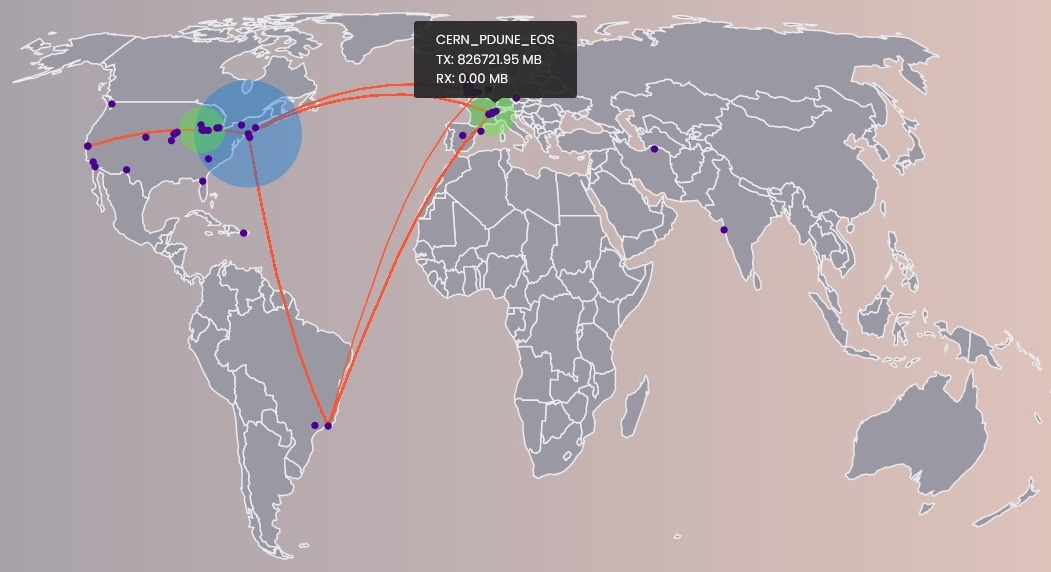
\includegraphics[width=\textwidth]{graphics/dune-firstVersionNotBad-show.jpg}

  \vspace{10mm}
  \today
    \vspace{15mm}
    
    {\large{The DUNE Collaboration}}
\end{center}

\cleardoublepage
\vspace*{16cm} 
  {\small  This document was prepared by the DUNE collaboration using the resources of the Fermi National Accelerator Laboratory (Fermilab), a U.S. Department of Energy, Office of Science, HEP User Facility. Fermilab is managed by Fermi Research Alliance, LLC (FRA), acting under Contract No. DE-AC02-07CH11359.
  
The DUNE collaboration also acknowledges the international, national, and regional funding agencies supporting the institutions who have contributed to completing this Conceptual Design Report.  
  }
%\includepdf[pages={-}]{tdr-authors.pdf}              add back in later    



\renewcommand{\familydefault}{\sfdefault}
\renewcommand{\thepage}{\roman{page}}
\setcounter{page}{0}

\pagestyle{plain} 

\setcounter{tocdepth}{4}  % Heidi to make the LBNC happy for now. 
\textsf{\tableofcontents}


\textsf{\listoffigures}

\textsf{\listoftables}
  \vspace{4mm}


\iffinal\else
\textsf{\listoftodos}
\clearpage
\fi

\renewcommand{\thepage}{\arabic{page}}
\setcounter{page}{1}

\pagestyle{fancy}

% Set how header/footers look
\renewcommand{\chaptermark}[1]{%
\markboth{Chapter \thechapter:\ #1}{}}
\fancyhead{}
\fancyhead[RO,L]{\textsf{\footnotesize \thechapter--\thepage}}
\fancyhead[LO,R]{\textsf{\footnotesize \leftmark}}

\fancyfoot{}
\fancyfoot[RO]{\textsf{\footnotesize Conceptual Design Report}}
\fancyfoot[LO]{\textsf{\footnotesize DUNE Computing Consortium}}
\fancypagestyle{plain}{}

\renewcommand{\headrule}{\vspace{-4mm}\color[gray]{0.5}{\rule{\headwidth}{0.5pt}}}

% Not all main documents have any citations.
% When not built in "final" mode, add in one citation just to let the
% document build.
% If, after substantial editing a main document still lacks any
% citations then it should have its whole bibliography removed.
%\ifdefined\isfinal\nocite{}\else\nocite{CD0}\fi
%\nocite{CD0} % REmoved 12/30/19


% see also preamble.tex
%\input{common/acronyms}

\cleardoublepage

% comment these lines out once we no longer need the example
% \setcounter{chapter}{-1}
% \chapter{Example Chapter (Anne Heavey)}
\label{ch:chap-id}

%%%%%%%%%%%%%%%%%%%%%%%%%%%%%%%
\section{Introduction}
\label{sec:chap-id:intro}

Sections and subsections should have labels for cross-referencing. Labels must be unique. See the suggested format.

See Figure~\ref{fig:required-label}. Notice that only the first word is capitalized in both the short and full captions.  

%%%%%%%%%%%%%%%%%%
\subsection{Dwords and the Glossary}
\label{sec:chap-id:intro}

The dwords are defined in common/glossary.tex. You use \verb|\dword{}| the same way, whether the term is defined as a ``newduneword'' or a ``newduneabbrev.''  A term defined as an abbreviation will show the full term the first time it's used in a chapter and just the abbreviation thereafter.  For instance:

As significant as this information is, it is the \dword{lsb}. In fact, compared to many things it is the \dword{lsb}.

You can also use \verb|\dshort{}| which doesn't hyperlink, but is useful in captions and headings to use the standardized rendering of a term.

%%%%%%%%%%%%%%%%%%
\subsection{Figures}
\label{sec:chap-id:intro}


Figure~\ref{fig:required-label} is the logo for \dword{dune}. 

\begin{dunefigure}
[Optional short caption for LoF]
{fig:required-label}
{Required full caption. Don't capitalize every word.}

\includegraphics[width=0.8\textwidth]{dunelogo_colorhoriz}
\end{dunefigure}

%%%%%%%%%%%%%%%%%%%%%%%%%%%%%%%
\section{My Amazing Widget}
\label{sec:chap-id:mywidget}

The string of percent signs just makes it easier to spot where new sections start.

Notice that all the main words in headings are capitalized.

Let's add a reference. I'm sure that this reference is useful somewhere, but not here~\cite{Acciarri:2016sli}.

Now let's add a ``dunetable.'' See Table~\ref{tab:table-label}.

\begin{dunetable}
[The LoT caption]
{cc}
{tab:table-label}
{The full caption that appears above the table.}
Rows & Counts \\ \toprowrule
Row 1 & First \\ \colhline
Row 2 & Second \\ \colhline
Row 3 & Third \\ % no \colhline on final row
\end{dunetable}

%%%%%%%%%%%%%%%%
\subsection{Numbers for my Widget}
\label{sec:chap-id:mywidget:num}

The following shows (1) how to do a bulleted list (notice the commas, the ''and'', and the period.  It also shows how to write different kinds of numbers.

\begin{itemize}
    \item 100 is written as \num{100},
    \item 1000 is written as \num{1000},
    \item 123.456 is written as \num{123.456},
    \item 1 plus or minus 2i is written as \num{1+-2i},
    \item 3 times 10 to the 45th is written as \num{3e45},
    \item 0.3 times 10 to the 45th is written as \num{.3e45} (keeps the decimal point before the 3), and 
    \item ''10, 20 and 30'' is written as \numlist{10;20;30}.
    \item 
\end{itemize}

%%%%%%%%%%%%%%%%
\subsection{Numbers with Units for my Widget}
\label{sec:chap-id:mywidget:numunit}

Here's how to do a numbered list and write numbers with units. 
\begin{enumerate}
    \item 120 GeV is written as \SI{120}{\GeV} or (more simply)  120\,GeV, and
    \item 4850 feet is written as \SI{4850}{\ft}.
\end{enumerate}

These and many others are defined in the file common/units.tex.

%%%%%%%%%%%%%%%%%%%%%%%%%%%%%%%
\section{My Second Amazing Widget}
\label{sec:chap-id:my2ndwidget}

If you have one section, you need at least two; same goes for subsections, etc. 

%%%%%%%%%%%%%%%%%%%%%%%%%%%%%%%
\section{More Information}
\label{sec:chap-id:moreinfo}

First, see Section~\ref{sec:chap-id:my2ndwidget} just to see how we do cross-sectional references.  The same goes for cross-chapter references, you just need to find the correct label for the chapter (or the section within the chapter).

More information is at \url{https://dune.bnl.gov/docs/guidance.pdf}.

Test the new defs file: \testanne

% \cleardoublepage


% We have decided to utilize the FP package for doing calculations and tracking constants in the CDR
% (e.g. the limit of annual data from ll active FD modules to permanent storage at FNAL is 30 GB/year)
% The template for a variable is this:
% "chapter""section"variable where both "chapter" and "section" are abbreviations
% with the Camel Caps used for readability
% Note that you should not override the use of a variable defined in generated/parameters.tex

% e.g. MonEtfDevPeople is the amount of effort for development in the ETF section of the Monitoring chapter
%  \FPset{MonEtfOpsPeople}{3.2}
%  \FPset{MonEtfDevPeople}{1.0}

% You can do floating point operations on constants defined in this manner:
% \FPadd\MonEtfTotalPeople\MonEtfOpsPeople\MonEtfDevPeople

% But note that floating point operations generate numbers with large precision and so you need to make
% sure to format numbers with printing them. In this example:

%\num[round-mode=places,round-precision=1]{\MonEtfTotalPeople}

% For FP set directly with \FPSet, then input precision will be maintained when printed.

%Global numbers for the entire document

\FPset{GlobalFDDataStorage}{30} % this is petabytes per year


\part{Overview} %Heidi
\documentclass[../main-v1.tex]{subfiles}
\begin{document}

%We have decided to utilize the FP package for doing calculations and tracking constants in the CDR
% (e.g. the limit of annual data from ll active FD modules to permanent storage at FNAL is 30 GB/year)
% The template for a variable is this:
% "chapter""section"variable where both "chapter" and "section" are abbreviations
% with the Camel Caps used for readability
% Note that you should not override the use of a variable defined in generated/parameters.tex

%Start of Introduction variables (Intro)

%End of Introduction varaibles

% Data and Processing Volume Estimates (DatVol)

\FPset{DatVolFDColdElecPrecision}{12} %number of bits in cold electronics digitization

% Use Cases (UseCase)

% Frameworks (Fra)

% Databases (DBs)

% Applications (App)

% Computing Model (CompMod)

% Site Resources (SiteRes)

% Data Placement (DataPla)

% Networking (Net)

% Workflow Examples (Wrkflw)


\chapter{Introduction \hideme{Schellman/Muether/Junk/Pennacchio needs numbers and figures update - SN added 2/19} }
\label{ch:intro}

%%%%%%%%%%%%%%%%%%%%%%%%%%%%%%%%
%\section{xyz}
%\label{sec:intro:xyz}  %% fix label according to section

\listoftodos
%\todo{Need to add discussion of physics requirements that drive computing}

%\todo{Need to add a section on simulation}
\todo{And brief subsection on solar/atmospheric/BSM physics}
\section{Mission Statement}
This document describes Software and Computing for the \dword{dune} experiment. Our emphasis on this document is on the development of the computing infrastructure needed to acquire, catalog, reconstruct, simulate and analyze the data from the \dword{dune} experiment and its prototypes. In this effort, we concentrate on developing the tools and systems that facilitate the development and deployment of advanced algorithms rather than the details of the algorithms themselves. Our goal is to, rather than prescribe particular algorithms, to provide resources that are flexible and accessible enough to support creative software solutions as \dword{hep} computing evolves
and provide computing that achieves the physics goals of the \dword{dune} experiment. %Kirby 

\section{Introduction \hideme{Schellman - draft based on CHEP paper}}\label{sec:intro-introduction}

%Anne The \dword{dune}  will begin running in the late 2020's. The goals of the experiment include 1) studying neutrino oscillations using a beam of neutrinos from Fermilab in Illinois to the the \dword{surf} in Lead, South Dakota, 2) studying  astrophysical neutrino sources and rare processes and 3) understanding  the physics of neutrino interactions in matter.
% from Anne: this is more standard:
The international \dword{dune} experiment, hosted by the U.S. Department of Energy's \dword{fnal}{},  will begin running in the late 2020's. It will consist of a \dword{fd} located about \SI{1.5}{km} underground at the \dword{surf} in South Dakota, USA, \SI{1300}{\km} from \dword{fnal}{}, and a \dword{nd} located on site at \dword{fnal} in Illinois. The \dword{dune} detectors will be exposed to the world's most intense neutrino beam originating at \dword{fnal}{}. A high-precision near detector, \SI{574}{m} from the neutrino source on the \dword{fnal} site, will be used to characterize the intensity and energy spectrum of this wide-band beam. The overriding physics goals of the \dword{dune} experiment are the search for leptonic \dword{cp} violation, the search for nucleon decay as a signature of a Grand Unified Theory underlying the Standard Model, and the observation of  \dwords{snb} from supernovae.
This document is intended to describe the conceptual design of the offline computing needed to accomplish these physics goals. %Kirby

\todo{How do I do this?}
 % I will concentrate on the neutrino oscillation and supernova capabilities of the experiment and the ways that they drive computing. 

When produced, the neutrino beam from \dword{fnal} will consist almost entirely of muon-type neutrinos. %Anne when produced. %HMS done 
Neutrinos are known to come in (at least) three flavors that can be distinguished by their interactions -- electron %Anne type 
neutrinos produce electrons when they interact via charged currents; muon neutrinos, muons; and tau neutrinos, tau particles.  But these flavors do not correspond to fixed mass states.  All three flavors of neutrinos are mixtures of mass states, much as  light polarized in the $x$ direction  can be considered a superposition of  $x^\prime$ and $y^\prime$ polarizations along  alternate axes rotated by 45 degrees.  When neutrinos propagate through space, it is the mass state that sets their wavelength and if the neutrino goes far enough, the multiple mass states  corresponding to the initial flavor state will get out of phase.  When the mixture is later probed about its flavor, it may be different than it was when the neutrino was produced. %Anne give a different answer than the neutrino that started out. %HMS done
This phenomenon is known as neutrino oscillation, and has been %Anne shown to exist %HMS observed 
observed in multiple experiments since it was first confirmed in 1998\cite{Kajita2006}.


\begin{dunefigure}
[Illustration of the neutrino flavor and mass states]
{fig:neutrinos}
{Illustration of the neutrino flavor and mass states.  The mass states are a superposition of the flavor states.  Courtesy the particlezoo.net.}
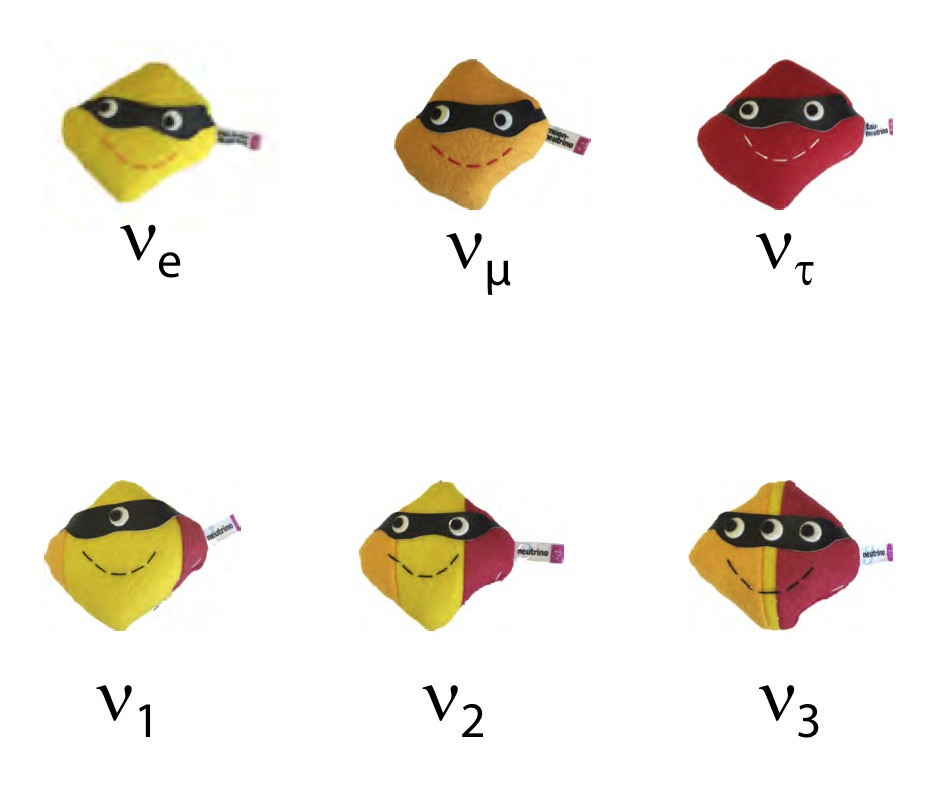
\includegraphics[height=6cm]{graphics/IntroFigures/Fig_01_neutrinos.jpg}
\end{dunefigure}



\begin{dunefigure}
[Electron neutrino appearance signal and background as seen in ArgoNeut]
{fig:Argoneut}
{Electron neutrino appearance signal (top) and background (bottom) as seen in the ArgoNeut experiment\protect{\cite{Acciarri:2016sli}}.  In the true appearance signal, an electron is seen emerging from the primary vertex, then showering.  In the background interaction, a muon neutrino enters and  produces a final-state muon and photons that propagate some distance before showering.}
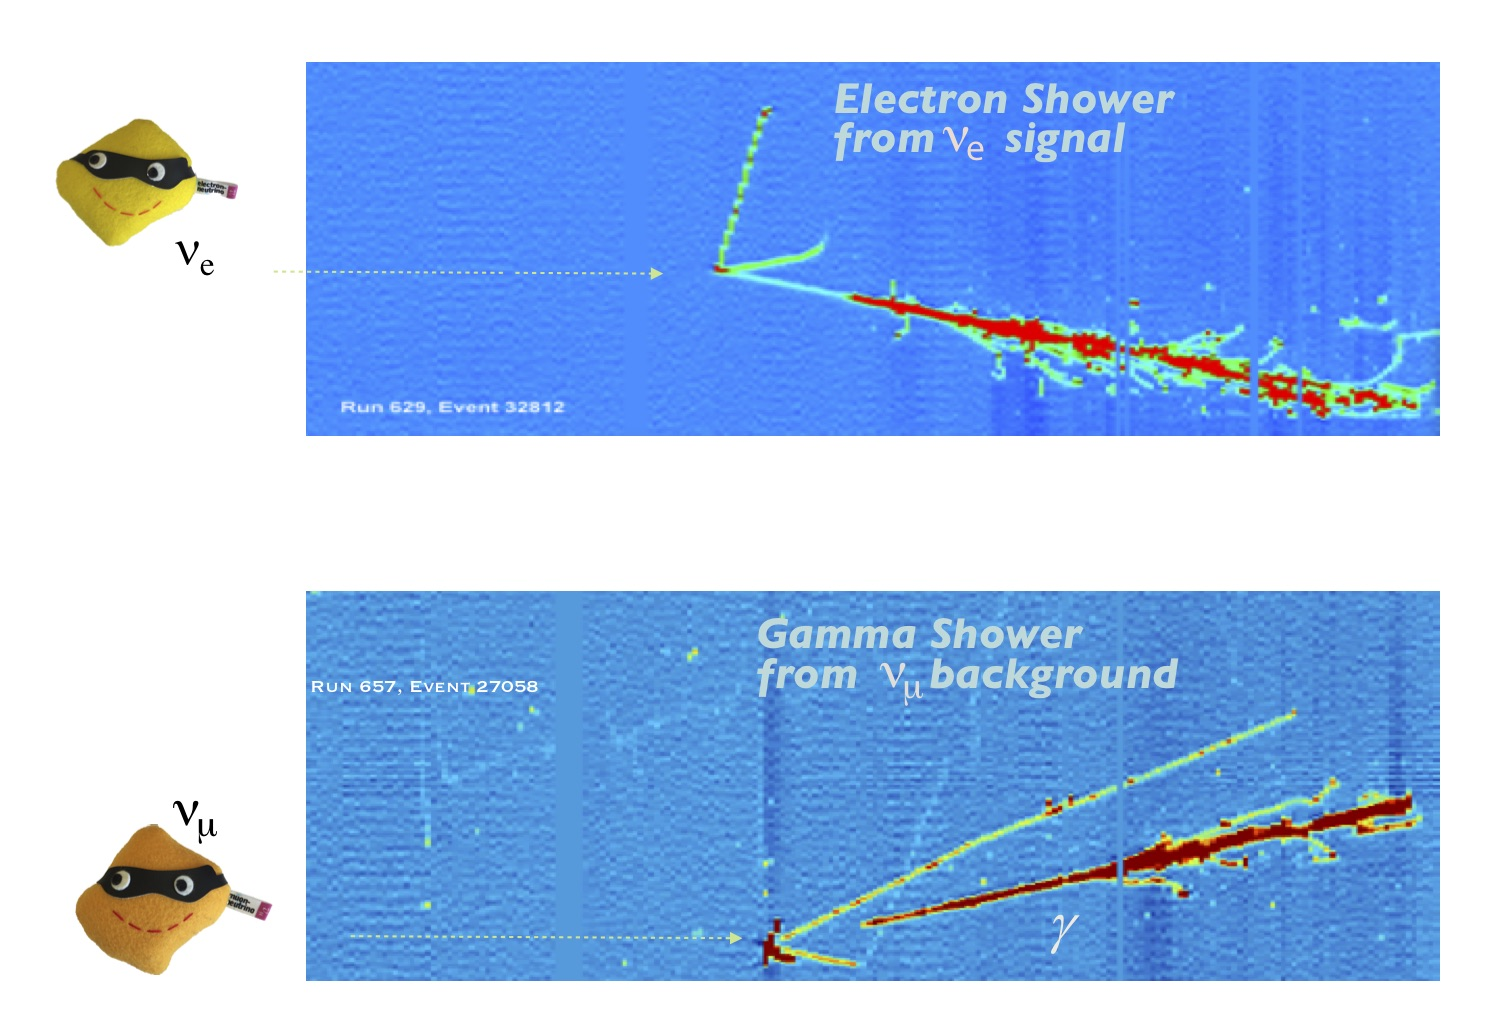
\includegraphics[trim={0cm 0.6cm 2.5cm 0.7cm},clip,height=6cm]{graphics/IntroFigures/Fig_02_Argoneut.jpg} 
\end{dunefigure}


DUNE,  in particular,   wishes to understand the conversion of the muon neutrinos created in Illinois%Anne Illinois 
into electron neutrinos at the \dword{fd} in the Homestake mine in South Dakota  %HMS made the change
and compare that conversion rate between neutrino and antineutrino beams. The location of the \dword{fd} and energy of the neutrino beam were chosen to maximize the oscillation effect.   A difference in the conversion rate for neutrinos and antineutrinos could be evidence for matter-antimatter asymmetry in the neutrino sector, a phenomenon called \dword{cpv}.  

To make these measurements, the experiment needs to be able to distinguish %Anne we need to be able to distinguish %Kirby "we->the experiment"
electron neutrino interactions  from the dominant muon neutrino interactions one would expect in the absence of oscillations.  %Anne Doing t
Doing this requires a very large detector, as neutrino interactions are intrinsically rare, but an extremely  fine-grained one, as well.  Noble liquid  time projection detectors, %HSM doesn't \dword{tpc} do that? 
which read out large transparent volumes of liquid by drifting electrons from interactions to charge-sensitive detectors through strong electric fields (\efield{s}), have the needed capabilities of extremely large scale and fine-grained resolution. The proposed DUNE far detector will instrument four  $14\times12 \times58$ meter volumes of \dword{lar} with readout granularity of $\sim$0.5\,cm.  The detector modules will be located 4850\,ft below the earth's surface to lower the rate of cosmic rays traversing the detector by orders of magnitude and thus allow sensitivity to very low-energy solar and astrophysical neutrinos, as well as the higher-energy neutrinos produced in the beam at Fermilab.  %Anne at Fermilab.
%Anne - I would reference the FD TDR Vol 1 where there is an excellent discussion of how LArTPC satisfy physics requirements.
Additionally, physics programs focused on nucleon decay, the detection of supernova burst, and other \dword{bsm} signatures take advantage of the large size of the detector and flexible readout window of the \dword{daq} and \dword{lartpc}. %Kirby


The neutrino beam from \dword{fnal} will be pulsed approximately once per second, 24 hours per day during running periods, % anne with 
yielding of order 15 million pulses per year.  Because neutrinos interact  extremely rarely, we expect to detect of order 7,000 neutrino interactions/year in each of the four 10\,kt detector modules%Anne located at the \dword{fd} site in South Dakota. 
\footnote{This is based on the beam repetition rate of 0.83 Hz and an estimated uptime for the accelerator complex of 56\% \cite{Abi:2020evt}.}.


%Anne - I would leave this out Construction of the detector halls and infrastructure for the large 10\,kt fiducial volume \dword{fd} modules is starting now, as are design and construction of detector readout modules.  
A full \dword{tdr} for the first far detector module, a horizontal-drift \dword{lartpc},
% Anne program has recently been completed and 
is available in references% anne in references 
\cite{DUNE:2020lwj, Abi:2020evt, Abi:2020oxb, Abi:2020loh}.
%The  \dword{dune} neutrino oscillation experiment will receive beam late in this decade with commissioning of the \dword{daq} %anne data acquisition 
The first far detector modules should go live late in this decade with commissioning of the data acquisition systems for the first far detector modules expected to start in 2027. % anne-28.  


\begin{dunefigure}
[A far detector cryostat and the horizontal drift \dshort{tpc} structure]
{fig:DUNESchematic} % Anne: label should have fig:
{(Left) A far detector cryostat that houses a 10\,kt \dword{fd} module with horizontal drift technology. The figure of a person indicates the scale.  (Right) A 10\,kt  \dword{dune} \dword{fd} \dword{spmod}, showing the alternating 58\,m long (into the page), 12\,m high anode (A) and cathode (C) planes, as well as the field cage that surrounds the drift regions between the anode and cathode planes. The modular anode and cathode planes are constructed of units called \dwords{apa} and \dwords{cpa}; the blank area on the left side was added to show the profile of a single \dword{apa}.}
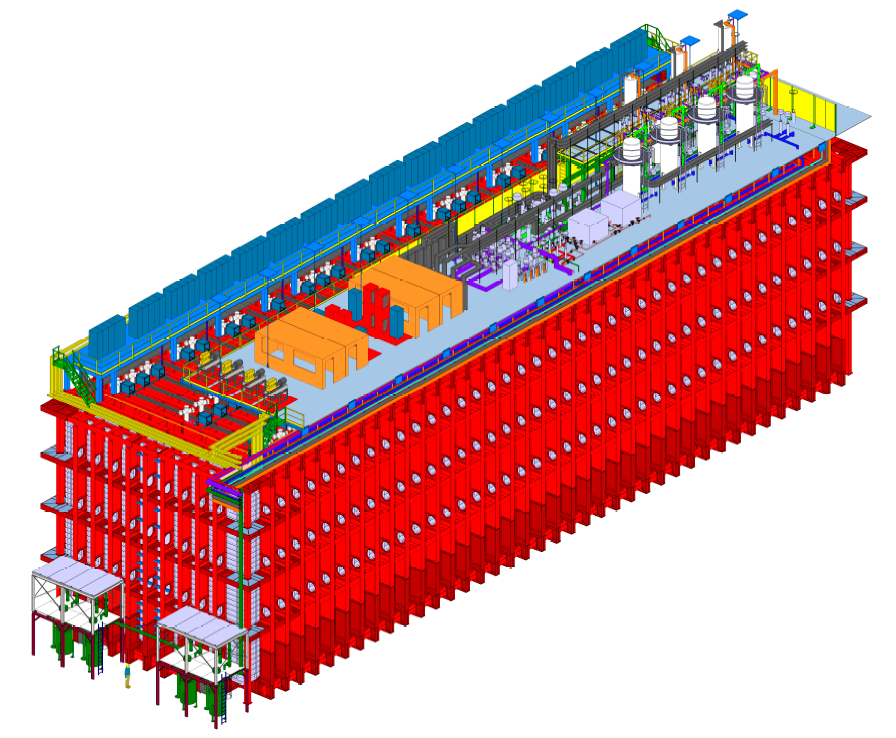
\includegraphics[height=0.35\textwidth]{graphics/IntroFigures/Fig_03a_cryostat-scale.png}
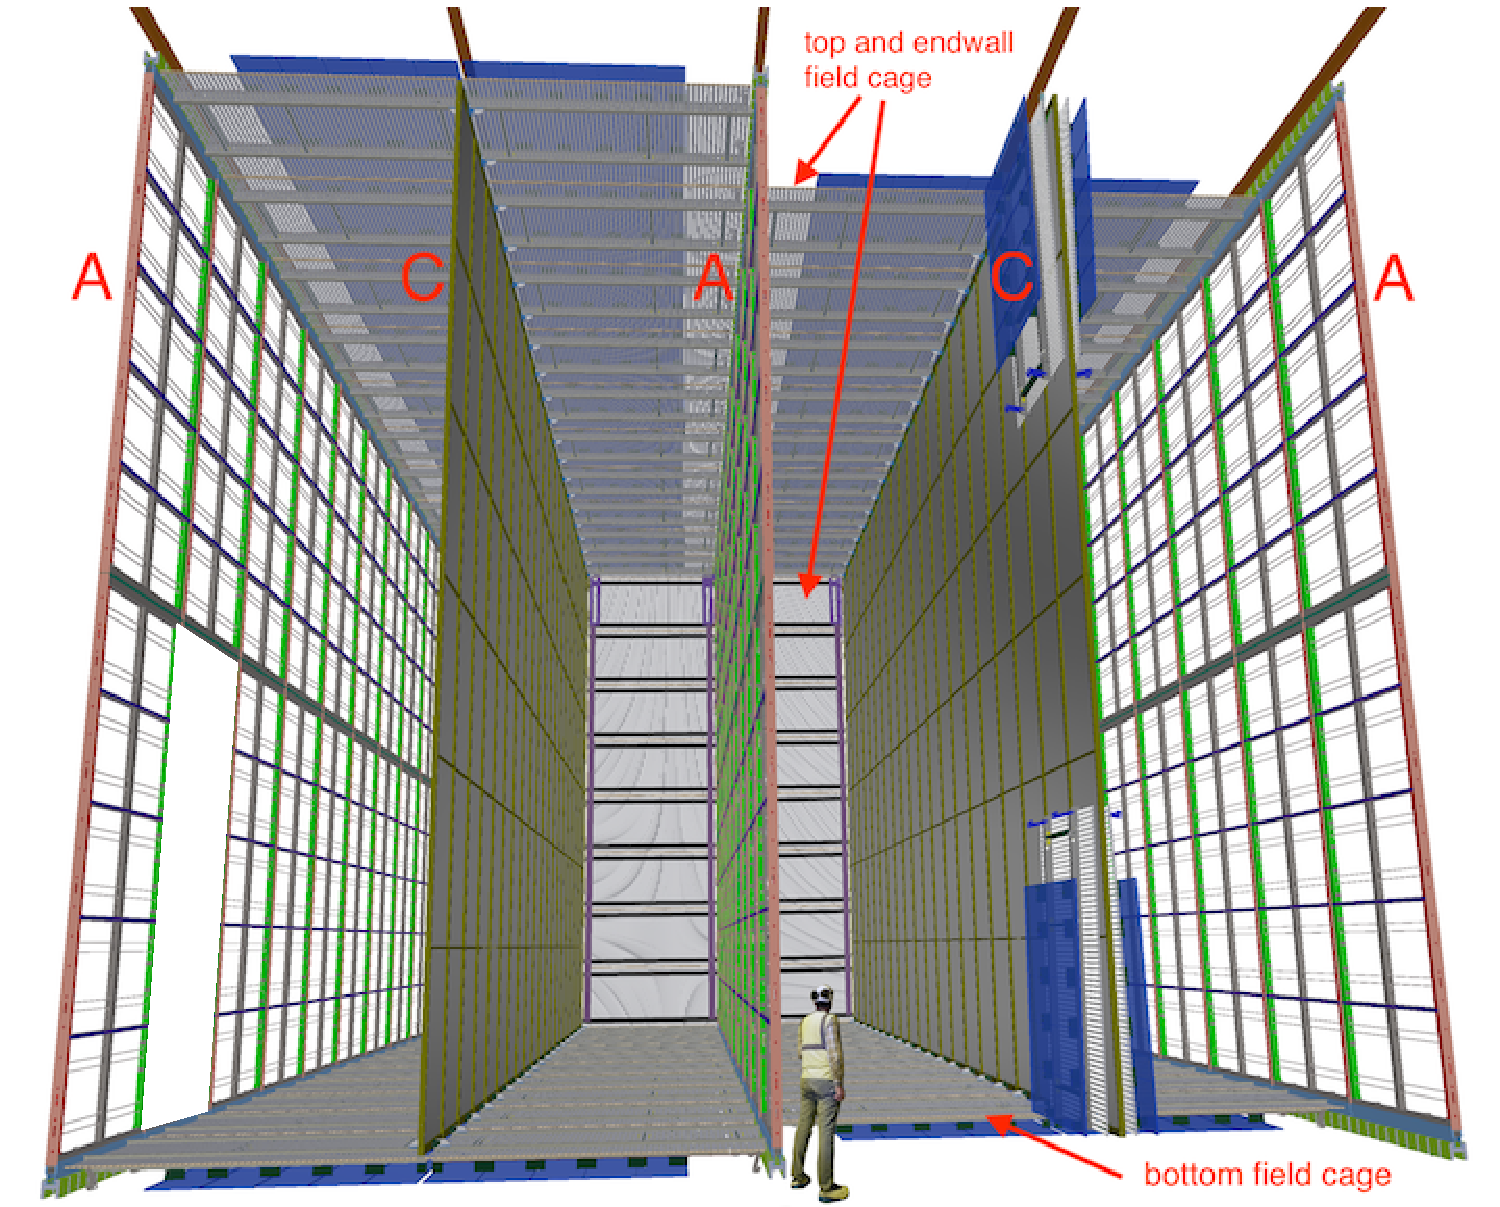
\includegraphics[height=0.35\textwidth]{graphics/IntroFigures/Fig_03b_DUNESchematic.pdf}
\end{dunefigure}


\section{ProtoDUNE tests at CERN  %anne ProtoDUNE tests at CERN 
\hideme{Schellman/Pennacchio-draft}}

Building an experiment of this size requires an extensive period of prototyping.   The Argoneut\cite{Acciarri:2018myr}, MicroBooNE\cite{microboone} and ICARUS\cite{icarus} collaborations have demonstrated the capabilities of \dwords{lartpc} for neutrino detection on scales between 1 and 500\,ton fiducial mass.  In preparation for the \dword{dune} experiment, a campaign for testing % anne proposed DUNE 
full-sized far detector components in 700\,ton-capacity cryostats %anne detectors 
in the \dword{ehn1} hadronic test beam at the \dword{cern} was launched in 2018.  Both \dword{sp} (horizontal drift) and \dword{dp} (liquid and gas, vertical drift) prototypes, called \dword{pdsp} and \dword{pddp}, were constructed and operated. %anne tested. % Kirby - I like this suggestion so included it with slight addition.
We have tested the full data taking chain from detector construction to full offline reconstruction and analysis of data, and the results have given considerable insight into the computing challenges for the full \dword{dune} experiment.

\subsection{\dshort{pdsp}} %anne ProtoDUNE Single Phase}
The \dword{pdsp} experiment began taking data at \dword{cern} in late 2018.  \dword{pdsp} %anne uses single-phase technology where 
collects ionization electrons %anne are collected 
directly from the liquid argon. The readout system consists of  %anne Anode Plane Assemblies (
\dwords{apa}.
%anne , which each have 3 layers of wires arranged in different directions. Each layer contains 800-1200  wires spaced 0.5 cm apart. Electrons drift from the original interaction in the Argon, through a strong electric field, to the wire planes and induce signals.  The location in the plane of hit wires gives one coordinate, the time the signal takes to drift to the wire from the original interaction measures a second coordinate.  The third coordinate is derived by combining information from overlaps of signals in the 3 different wire layers.  Signals are amplified electronically and then digitized.  
% anne: From the TDR:
Each \dword{apa} consists of an alumninum frame with three layers of active wires, strung at angles chosen to reduce ambiguities in event reconstruction, that form a grid on each side of the \dword{apa}. The relative voltage between the layers is chosen to ensure transparency to the drifting electrons of the first two layers ($U$ and $V$). These layers produce bipolar induction signals as the electrons pass through them. The final layer ($X$) collects the drifting electrons, resulting in a unipolar signal. The pattern of ionization collected on the grid of anode wires provides the reconstruction in the remaining two coordinates perpendicular to the drift direction 
Figure \ref{tpcconcept} illustrates the principle of operation. %anne of a generic \dword{lartpc}.

Horizontal drift \dword{sp} technology with \dword{apa} readout, similar to those used in \dword{pdsp}  will be used for the first of the four \dword{fd} modules. 


\begin{dunefigure}
[Signal formation in a LArTPC with three wire planes]
{tpcconcept} % Anne: label should have fig:
{Diagram  from  \protect{\cite{ Acciarri:2017sde}}  illustrating the signal formation in a \dword{lartpc} with three wire planes~\cite{Acciarri:2016smi}. For simplicity, the signal in the first (U) induction plane is omitted in the illustration. }
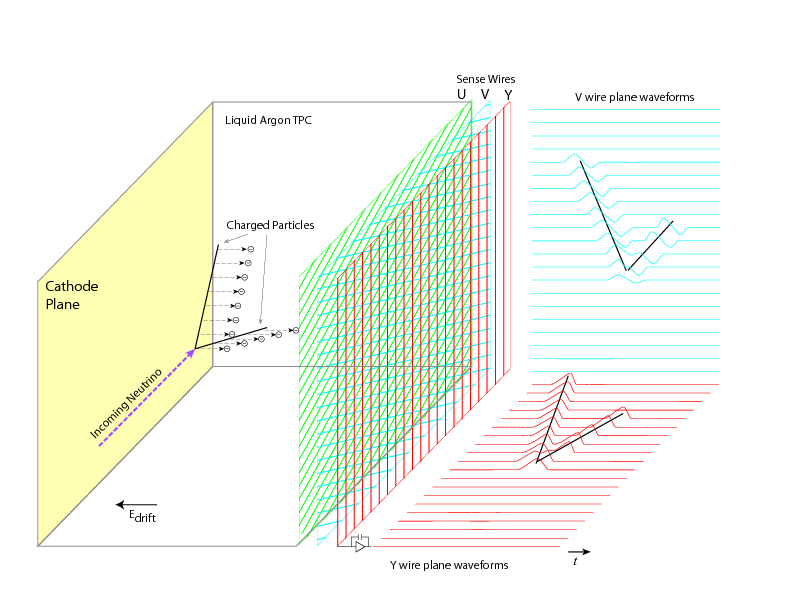
\includegraphics[trim={0cm 0.6cm 2.5cm 0.7cm},clip,height=8cm]{graphics/IntroFigures/Fig_04_LArTPC_Concept.png}
\end{dunefigure}

The \dword{pdsp} detector, immersed in 700\,tons of \dword{lar}, consists of %anne a 700 ton volume of liquid argon with 
a cathode plane in the center and sets of three \dwords{apa} mounted side-by-side on %anne each  edge 
either side of the liquid volume, creating a horizontal \efield. %The \efield is horizontal so this technology is designated \dword{hd}.   
The maximum drift distance is  3\,m with  a nominal voltage of 180\,kV  across that distance.  Each \dword{apa} has 2560 channels and each channel reads out a 12\,bit \dword{adc} every 0.5\,$\mu$sec. %anne  For \dword{pdsp} the readout time appropriate for a 3 m drift was set to 3 msec, 
The appropriate readout time for this configuration was determined to be 3\,s, resulting in 6000 12\,bit samples per channel. 
\todo{Anne: previous sentence doesn't make sense to me. 6000 per channel per readout window?}
The total data size for six \dwords{apa} is thus 140\,MB with additional header and data from photon and external tagging systems, bringing the nominal \dword{tr} size up to about 180\,MB.  Lossless compression of the \dword{tpc} readout data was implemented in the \dword{daq}, resulting in a final compressed event size of about 75\,MB. 


%\subsubsection{Trigger Records \hideme{draft}}

Neutrino experiments, and in particular \dword{tpc} based experiments, may or may not have internal triggers but they are generally read out over a fixed time window.  For \dword{protodune}, \dword{microboone}, \dword{minerva} and the \dword{minos} and \dword{nova} near detectors, a readout generally corresponds to either the 10\,$\mu$sec beam spill or a multi-msec \dword{tpc} drift time.  Within that time span, multiple beam, cosmic ray or rock muon interactions may occur within the active detector volume.  Thus the unit of detector readout, the \dword{tr}, does not correspond directly to a single interesting interaction, but to a group of interactions. The processing frameworks that we use have grown out of collider experiments and are based on the concept of an ``event,'' generally a beam crossing, that is processed as a unit.  DUNE prefers to use the term ``trigger record'' rather than ``event'' for the unit of processing, as it avoids confusion between an interaction ``event'' and a readout ``event.''  


The test beam ran at rates of up to 25\,Hz over a period of six weeks at beam momenta between 0.5 and 7\,GeV/c.  Time-of-flight and Cherenkov counters in the beamline provided beam flavor tagging.  Around 8M total ``physics'' records were written, with around 3M having beam tag information.  In total  850\,TB of raw test beam data were written, along with one PB of commissioning and cosmic data. These data were successfully catalogued and written to storage at both \dword{cern} and \dword{fnal} at rates of up to 2\,GB/sec.   

Thanks to significant prior effort in the \dword{lartpc} %Kirby fixed \todo{Anne:is it really \dword{lartpc}?}
computing and algorithms community, reconstruction software was ready to go. The first reconstruction pass began soon after data taking started and was complete within two weeks of the end of data taking.  These results were extremely useful in demonstrating the capabilities of the detector; they summarized in Volume II of the \dword{sphd} \dword{tdr}\cite{Abi:2020evt}.  A second pass, with improved treatment of instrumental effects ranging from stuck bits, to \twod deconvolution, to correction for space charge effects, was completed in late 2019. Another pass with major improvements to the electrostatic modeling and reconstruction algorithms was launched in 2021. 

%\dword{pdsp} Reconstruction - from raw data to beam interactions and cosmics full reconstructed with 80-90\% efficiency - has been performed twice over the 8M interactions recorded during the test-beam runs. 
Figure~\ref{deconvolution} illustrates the signal processing stage of reconstruction, where raw \dword{adc} signals have noise and stuck bits removed and are then deconvoluted to yield Gaussian hit candidates. An important aspect of the reconstruction of APA based \dword{lartpc}s is the need for a 2D signal processing and deconvolution to include extending the time domain beyond the interaction timing window to account for FFT edge effects. The impacts the reconstruction algorithms and framework processing. Figures~\ref{wire-cell-bee} and~\ref{pandora} illustrate full pattern recognition and event reconstruction. 

While \dwords{lartpc} benefit from fine granularity and a uniform detector medium, it is possible for diffusion, argon purity \todo{variation?}, fluid flow and the build up of space charge in the active medium %anne can all 
to introduce distortions into the detector response.  These effects have all been simulated and tested in the \dword{pdsp} data. 

Compressed raw input trigger records were of order 75\,MB in size and took 500-600 seconds to reconstruct, of which around 180\,s was signal processing and the remainder high-level reconstruction dominated by 40-60 cosmic rays per readout.  Memory footprints for data processing ranged between 2.5 and 4\,GB.  Output   record sizes were reduced to 22\,MB by dropping the raw waveforms after hit finding.   Data reconstruction campaigns took of order 4-6 weeks (similar to the original data taking) and utilized up to 15,000 cores on \dword{osg} and \dword{wlcg} resources.  Job submission was done through the \dword{poms}\cite{poms} job management system developed at \dword{fnal}. \dword{poms} supports submissions to \dword{fnal}-dedicated resources and selected \dword{osg} and \dword{wlcg} sites.  Figure \ref{sites} shows the distribution of wall hours used for reconstruction in 2019.
These metrics have influenced the ideas regarding memory utilization, event data model, and workload/workflow management in this document.

For reconstruction, data were streamed via {\tt xrootd}\cite{Behrmann:2011zz} from \dword{dcache} storage at \dword{fnal} to the remote sites. Despite individual processing jobs taking 15-30 hours to complete, network interruptions rarely caused job failures. 


\begin{dunefigure}
[Raw and deconvolved induction U-plane signals before and after signal processing]
{deconvolution} % Anne: label should have fig:
{Comparison of raw (left) and deconvolved induction U-plane signals (right) before and after 
the signal processing procedure from a \dword{pdsp} \dword{tr}. The bipolar shape with red (blue) color representing
positive (negative) signals is converted to the unipolar shape after the \twod deconvolution.}
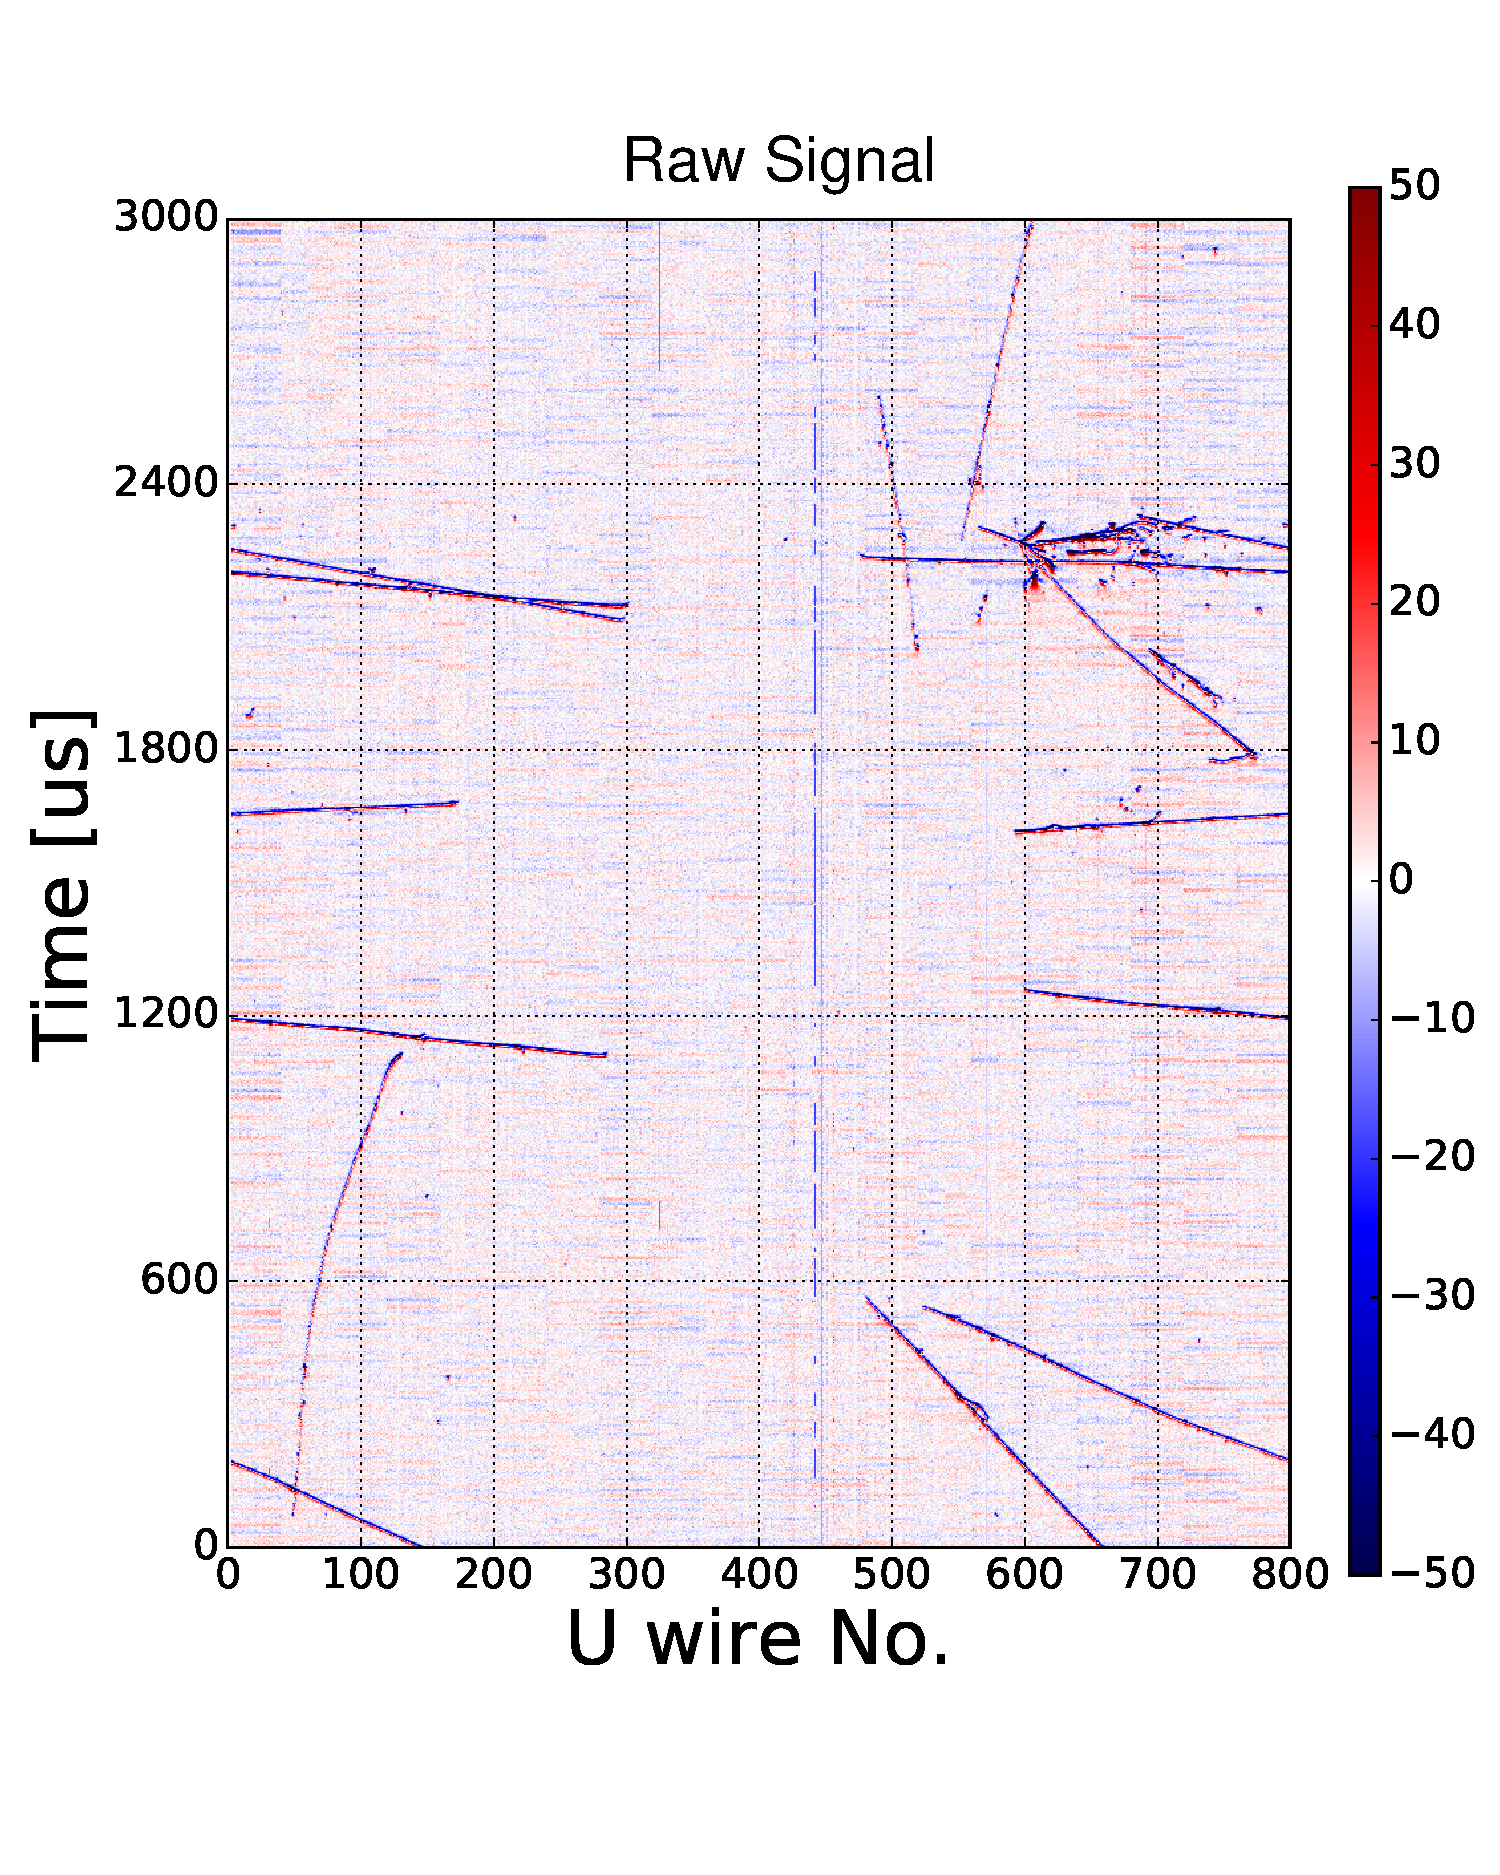
\includegraphics[width=0.49\textwidth]{graphics/IntroFigures/Fig_05a_protodune_raw_u.pdf}
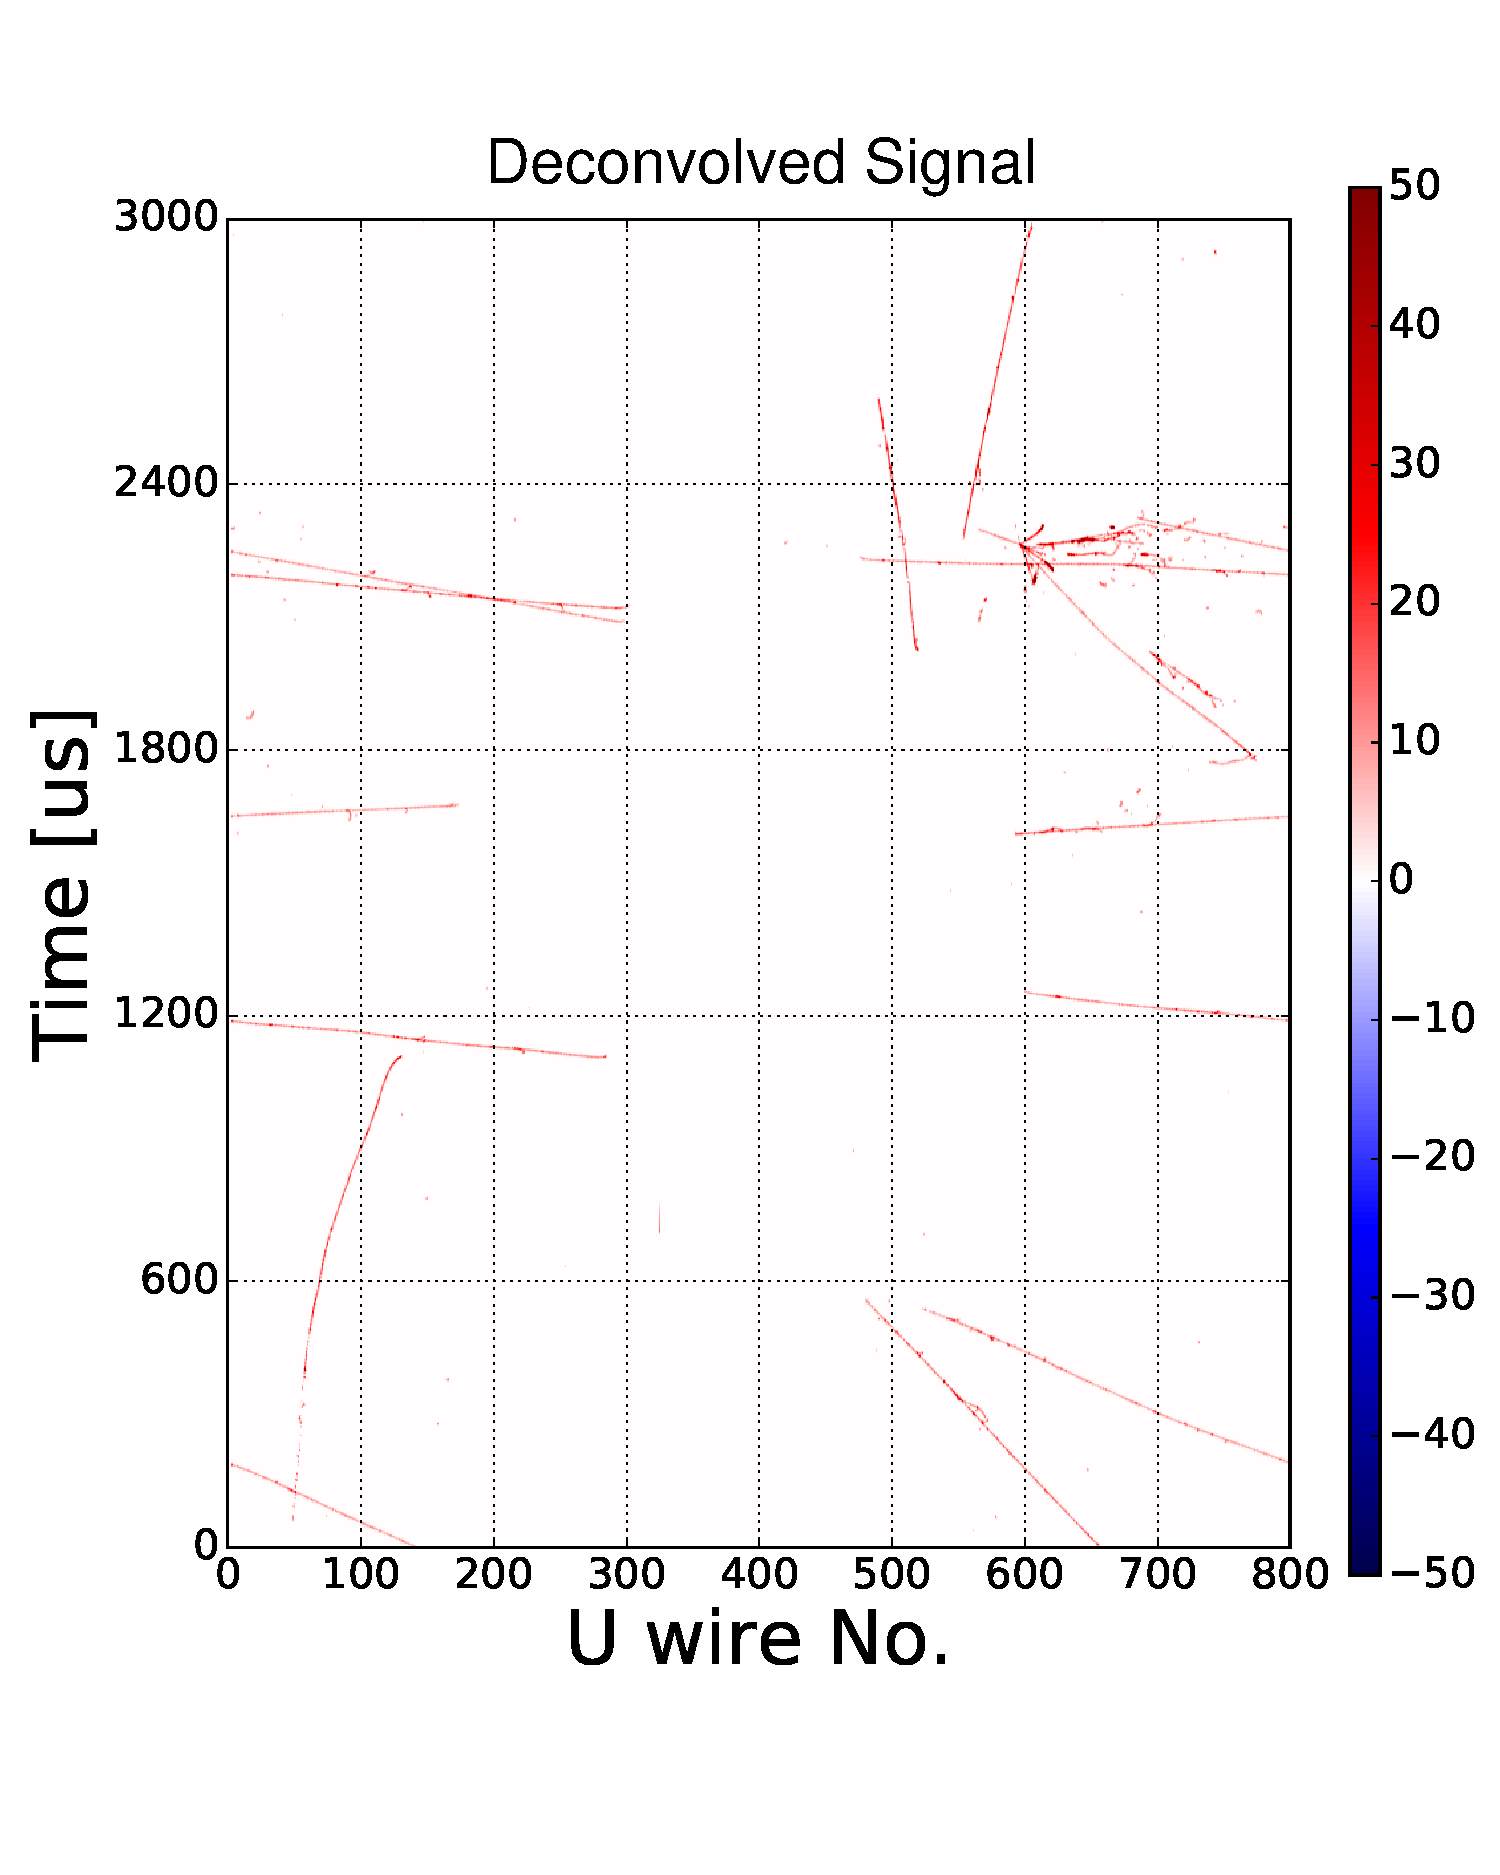
\includegraphics[width=0.49\textwidth]{graphics/IntroFigures/Fig_05b_protodune_decon_u.pdf}
\end{dunefigure}

\begin{dunefigure}
[Cosmic rays and beam interaction in \dshort{pdsp}]
{wire-cell-bee} % Anne: label should have fig:
{The \dword{pdsp} detector (gray box) showing 
the direction of the particle beam (yellow line on the very far left) and the outlines of the six \dwords{apa}. Cosmic rays
can be seen throughout the white box, while the red box highlights the beam region of interest with an interaction of the 7\,GeV beam. 
The \threed points are obtained using the Space~Point~Solver reconstruction algorithm.}
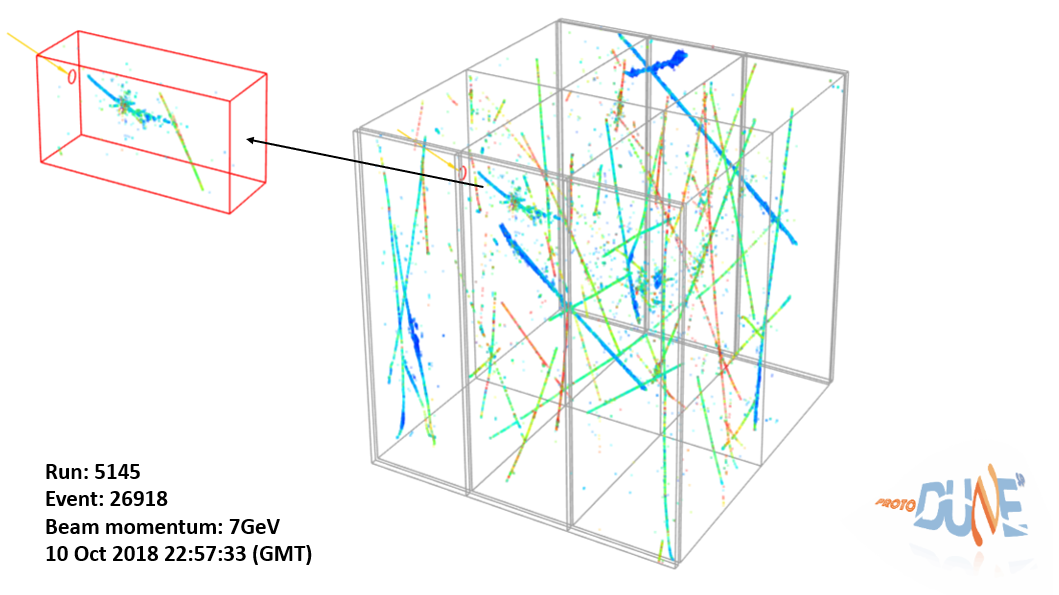
\includegraphics[width=0.9\textwidth]{graphics/IntroFigures/Fig_06_bee_event.png}
\end{dunefigure}


\begin{dunefigure}
[Pandora reconstruction of cosmic rays and beam interaction in a \dword{pdsp} trigger record]
{pandora}
{Pandora \protect{\cite{Acciarri:2017hat}} reconstruction of cosmic rays and beam interaction in a \dword{pdsp} \dword{tr}. The left side of the figure shows the full detector volume with all interactions, including cosmic rays and the right side shows the identified beam interaction.}
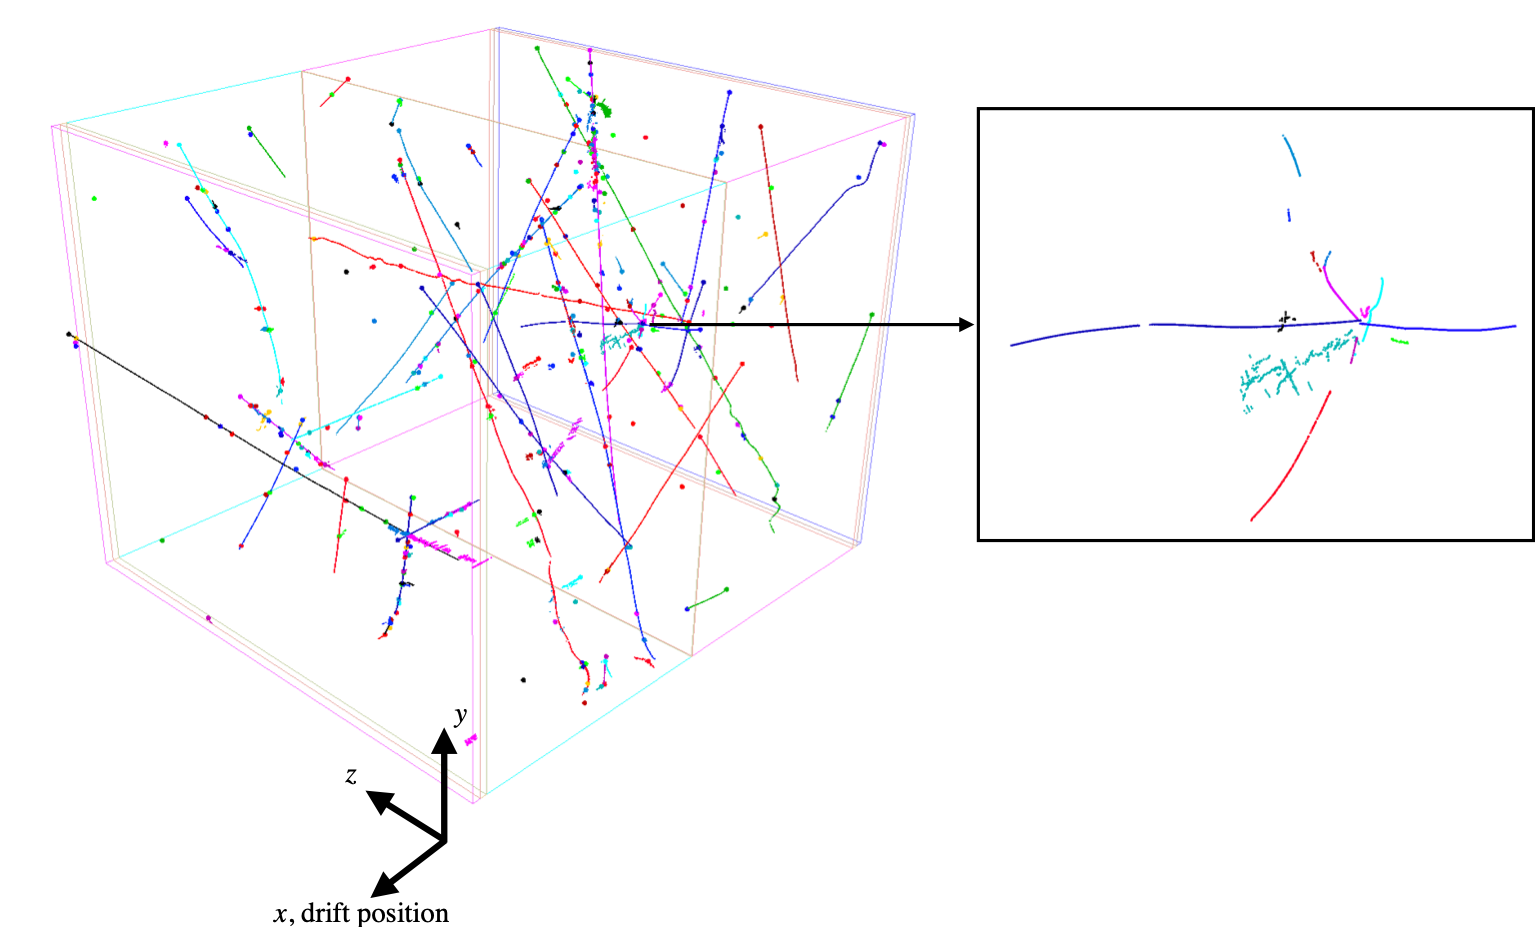
\includegraphics[width=0.8\textwidth]{graphics/IntroFigures/Fig_07_pandora.png}
\end{dunefigure}


\begin{dunefigure}
[Reco/sim processing distribution across sites for DUNE production, 2019]
{sites} % Anne: label should have fig:
{Reconstruction and simulation processing distribution across sites for DUNE production in calendar 2019.  The inner circle shows national contributions while the outer circle shows individual site contributions.}
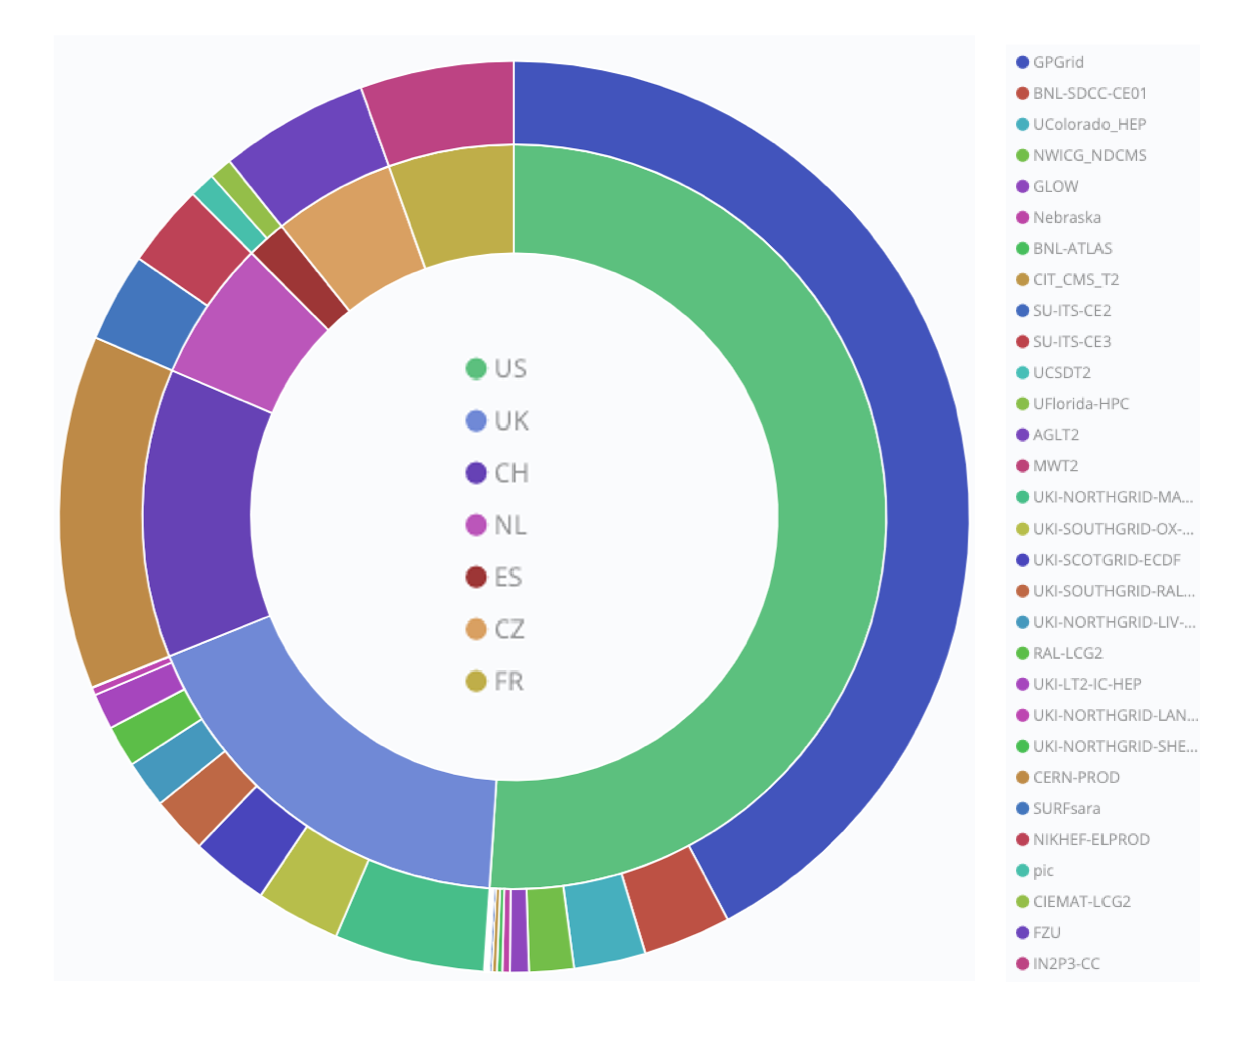
\includegraphics[height=0.65\textwidth]{graphics/IntroFigures/Fig_8.pdf}
\end{dunefigure}

\subsection{ProtoDUNE Dual-Phase\hideme{Pennacchio - draft}}

%The \dword{pddp} detector began taking data using cosmic rays in August 2019.  Thanks to preceding data challenges, those data have been successfully integrated into the full data cataloging and reconstruction chains and are now being reconstructed as they arrive.   The \dword{pddp} technology locates the readout systems above a thin layer of argon gas above the liquid argon surface.  This gas layer allows an external electric field to accelerate the electrons and produce gas amplification.  The result is a substantial increase in signal-to-noise in the resulting signals, at the cost of longer electron drifts from the bottom of the liquid volume.  Figure \ref{dpevent} illustrates early data from \dword{pddp}. 

In parallel with the single-phase horizontal-drift detector tests, a vertical drift  \dword{dp} readout prototype (\dword{pddp})
in a similar cryostat was also  tested.  \dword{pddp} was not exposed to beam but ran on cosmics in 2019 and 2020. 

The basic operating principle of \dword{pddp} is shown in Figure~\ref{dp_principle}. Charged particles that traverse the active volume of the \dword{lartpc} ionize the medium while also producing scintillation
light. The ionization electrons drift vertically upward %anne in the vertical direction 
toward an extraction grid just below the liquid-vapor interface. 
After reaching the grid,
an \efield stronger than the drift field extracts the electrons from the liquid up into the gas phase.
Once in the gas, electrons encounter micro-pattern gas detectors, called \dwords{lem}, with high-field regions. The \dwords{lem} amplify the electrons in avalanches that occur in these
high-field regions. The amplified charge is then collected and recorded on a \twod anode consisting
of two sets of 3.125\,mm pitch gold-plated copper strips that provide the $x$ and $y$ coordinates (and
thus two views) of an interaction.   

\begin{dunefigure}
[Principle of \dshort{dp} readout and parameters for extraction]
{dp_principle} % Anne: label should have fig:
{Principle of \dword{dp} readout (left), and thicknesses and HV values for electron extraction from liquid to gaseous argon, their
multiplication by \dwords{lem}, and their collection on the x and y readout anode plane (right) The HV values are
indicated for a drift field of 0.5\,kV/cm in LAr.}
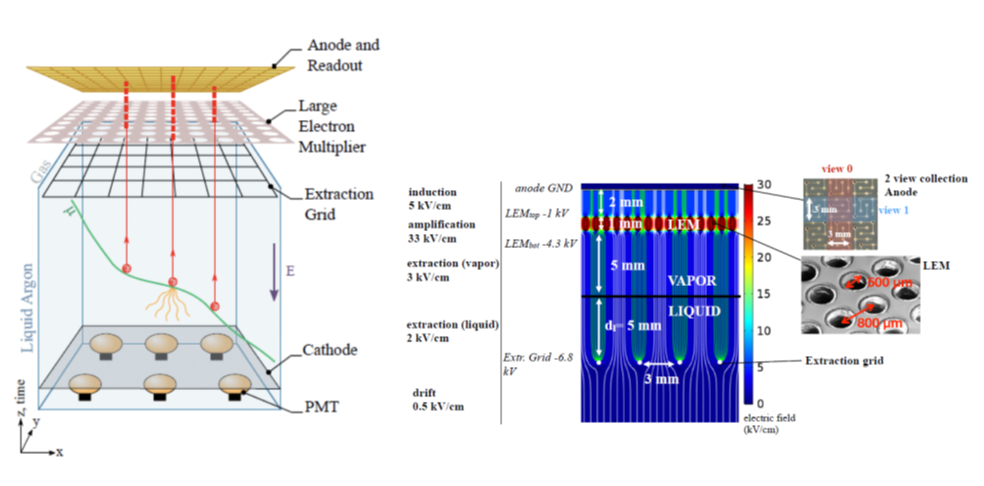
\includegraphics[width=0.85\textwidth]{graphics/IntroFigures/Fig_11_protodune-dp-principle.png}
\end{dunefigure}

The readout area surface is \SI{6x6}{m}, subdivided into four $3\times3$ m$^2$  \dwords{crp}. Each \dword{crp} is an independent detector element %anne insuring 
that performs electron extraction, amplification, and collection. 
The 7680 readout channels are read by   12\,bit \dwords{adc} every 0.4\,$\mu$sec. 
The \dword{pddp} detector   consists of a 700\,ton volume of \dword{lar}, with  a vertical drift length of 6\,m, corresponding to a full drift window of 4\,ms (10,000 samples).


The \dword{pddp} detector began taking cosmic ray data in August 2019. Thanks to preceding data challenges, these data have been successfully integrated into the full data cataloguing and reconstruction chain and were   reconstructed as they become available.
A total of 1.45M \dwords{tr} were collected; the size of the raw data files (run sequence files) was 2.3\,GB, each file containing 10 \dwords{tr}. Cosmic ray data are displayed in Figure~\ref{dpevent}: on
the left a horizontal muon track is shown with the corresponding waveform on a channel, giving an
idea of the low noise conditions. A \dword{tr} including an electromagnetic shower and two muon decays
and a \dword{tr} with an example of multiple hadronic interactions in a shower are shown on the right.

%samweb list-files "data_tier raw and run_type protodune-dp " --summary
%File count:	143583
%Total size:	334,415,580,215,147
%Event count:	1454065

 
\begin{dunefigure}
[Cosmic ray data from \dshort{pddp}]
{dpevent} % Anne: label should have fig:
{Cosmic ray data from the \dword{dp} prototype, \dword{pddp}.}
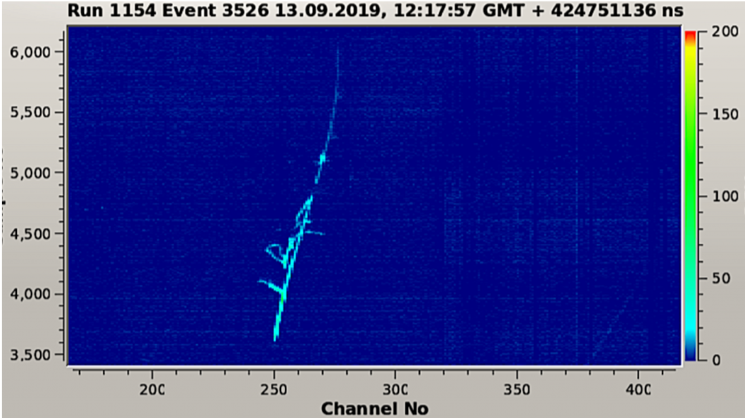
\includegraphics[width=0.85\textwidth]{graphics/IntroFigures/Fig_09_protodune-dp-event.png}
\end{dunefigure}


All data ($\sim$\,330\,TB) taken during different campaigns   have been copied to \dword{fnal}. A subsample is composed of data sets taken during detector transient conditions, motivated by various specific testing needs;  all cosmic ray data taken in well defined and stable detector conditions in 2019 and 2020 ($\approx$\,377K events) have been processed with \dword{larsoft} by performing the reconstruction of hits and \twod tracks. A second pass, including \dword{pandora} reconstruction algorithms, started in spring 2021. 
The memory footprint is between 1.9 and 2.5\,GB
As for \dword{pdsp}, job submission was done through \dword{poms}.

In the fall 2020 the \dword{dp} design evolved to the \dword{spvd} concept. The \dword{spvd} incorporates many of the design aspects developed for the \dword{dp}, such as the \dwords{crp};   the  main  difference  with  respect  to  the  \dword{dp}  design  is   the  removal  of  the  extraction  stage  to  the  gas  phase  and  the  subsequent  charge  amplification  stage.  %anne  This  change eliminates the grid immersed in the liquid and biased at high voltage in order to define the field needed to transfer the electrons from the liquid to the gas phase and the \dwords{lem} used to amplify the signal.
This eliminates the grid biased at high voltage (to transfer the electrons from the liquid to the gas) and the \dwords{lem} used to amplify the signal in the gas. The \dword{spvd} \dwords{crp} %anne keeps the concept of charge readout performed 
perform charge readout using %anne with  strips implemented on segmented 
perforated \dword{pcb} anodes with finely segmented strip electrodes %anne while replacing the \dword{lem} micro-pattern detectors, which operated in the argon gas phase and coupled to the anode printed circuit boards with charge collection strips, with perforated anodes 
that are immersed in the \dword{lar}
 

\begin{dunefigure}
[Vertical drift solution with \dshort{pcb}-based charge readout]
{fig:vd_principle}
{Vertical drift solution with \dword{pcb}-based charge readout}
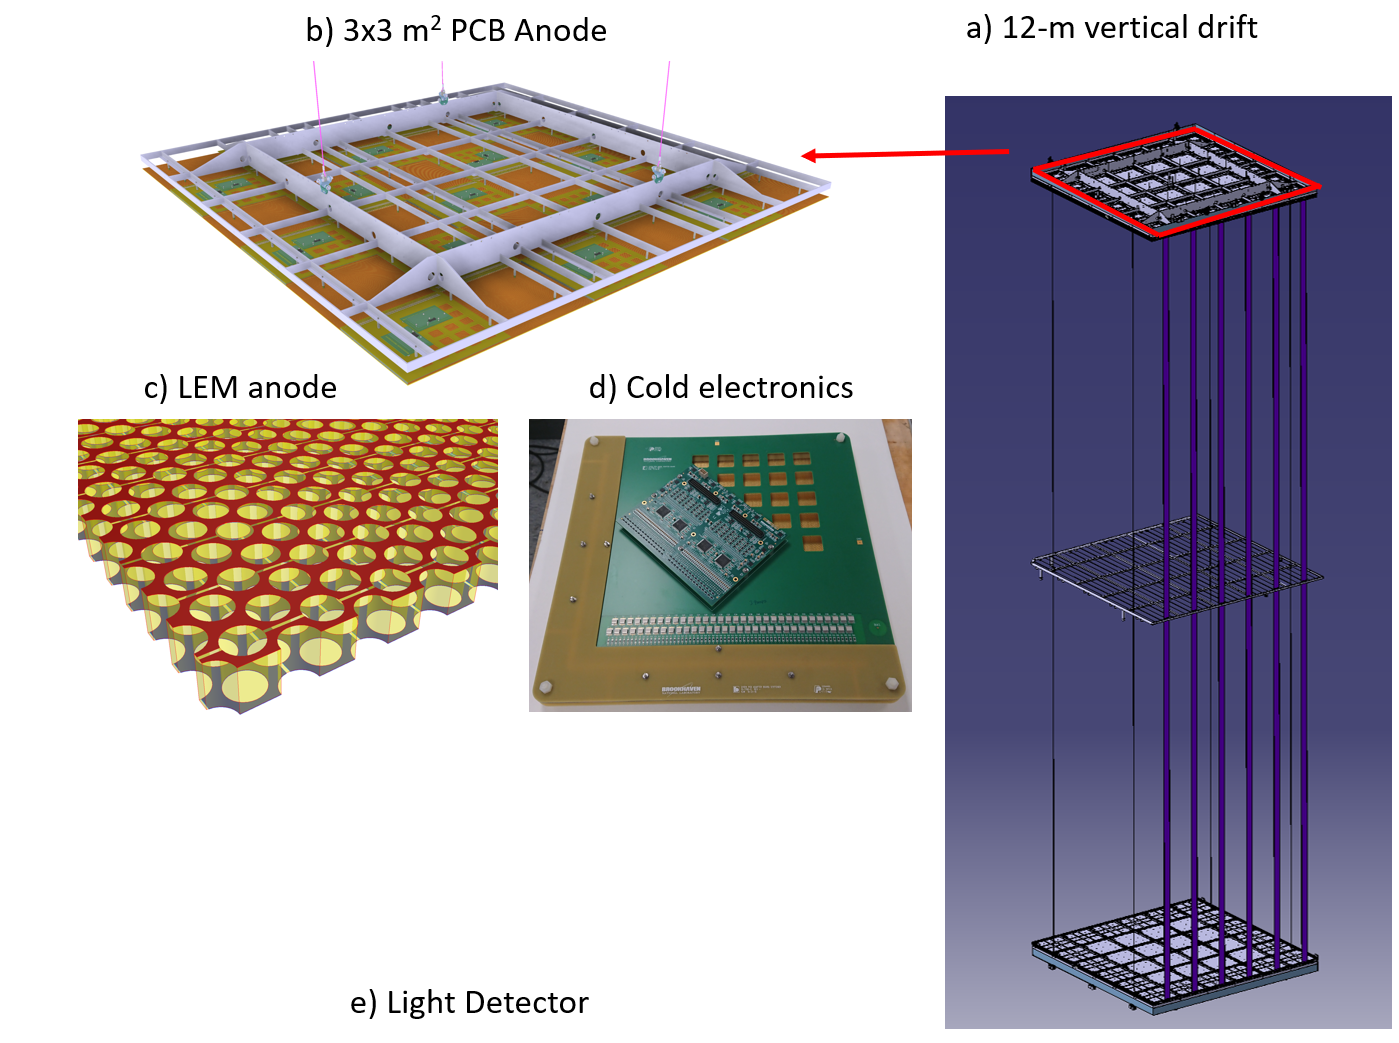
\includegraphics[width=0.85\textwidth]{graphics/IntroFigures/Fig_13_VD_solution.png}
\end{dunefigure}

 Figure \ref{fig:vd_principle} illustrates the \dword{pcb}-based charge readout concept. The electron drift direction is vertical.
Two separate drift volumes of 6.5\,m are defined by a cathode plane at roughly mid-height in the
detector volume. Ionization electrons above the cathode will drift upwards; ionization electrons in the liquid below the cathode will drift downwards.
The \dword{spvd}  prototype components have undergone testing starting in 2021 with a small \coldbox.  A full prototype, known as \dword{mod0}, is expected to be completed and  installed 
 inside the \dword{np02} cryostat in 2022 and 2023. Long-term operation and full characterization with a charged particle beam will follow. 



\subsection{Conclusions from prototype tests \hideme{Schellman draft}}

\dword{protodune} %anne prototype 
runs are ongoing and will continue through beam tests in 2022-23 at \dword{cern}.  Data cataloguing, movement and storage techniques were tested before the start of the \dword{pdhd} and \dword{pdvd}  runs and were able to handle the full rate of the experiments.   Reconstruction algorithms were also in place on time and %anne were able to 
produced early results that led to increased understanding of the detector and improved calibrations for a second iteration.  These tests also identified some deficiencies in our infrastructure, including incomplete schemes for the transmission of configuration and conditions information between hardware operations and  offline computing.  The test beam runs have been extremely valuable in allowing us to determine which variables are important to transmit and in designing improved systems for gathering and storing that information. 

An additional beam run of  \dword{pdsp} is planned for 2022-23, with a cosmic test of the \dword{spvd} design to follow in 2023-24, allowing further development and testing of our computing infrastructure before the full detector comes online in the late 2020s. 

%\section{ProtoDUNE Simulation} % anne discussion 
%\hideme{Yang-needed}

\section{On to full DUNE \hideme{Schellma-draft}}\label{sec:intro-fd}

The full DUNE \dword{fd} will begin with one \dword{sphd} module to be installed %anne at Homestake 
starting in the middle of  this decade.  A second \dword{spvd} module will be installed and commissioned in parallel.  High-intensity neutrino and antineutrino beams should arrive after a year or so of commissioning of the detector and \dword{lbnf} beamline.  The first %anne \dword{hd} 
module will %anne largely resemble 
be a scaled up version of \dword{pdsp} with 150 \dwords{apa} distributed 2-deep %anne 2-deep? at 
the length of the cryostat, down the center and along the long walls. %\anne edges of the cryostat.   
The argon volume will be $15\times14\times62$\,m$^3$ with a total (fiducial) mass of 17\,kt (10\,kt).  Section~\ref{sec:est:FD} summarizes the expected event rates and data volumes for the first two modules.  Two additional detector modules, possibly with updated or novel technologies %anne, beyond the first two 
will be added later. For now, we assume that data volumes and rates coming from other technologies will not exceed %anne be less than or equal to the single-phase values. 
the values for the \dword{sphd} or \dword{spvd}.



The detector should be sensitive to neutrino interactions and radioactive decays above an energy threshold of order $\sim 5$\,MeV.  Unambiguous triggering may require a somewhat higher threshold  to avoid false triggers due to $^{39}$Ar decays,  but beam interactions in the 500-10,000\,MeV range should have almost perfect detection efficiency. Sophisticated triggering algorithms should also allow standalone detection of astrophysical sources, including higher-energy solar neutrinos and \dword{snb} candidates. 

The data rates will be dominated by 4,500 cosmic rays expected per module/day.  These events are vital for monitoring and aligning the detector. %anne aligning?
The next most significant source of events will be calibration campaigns with radioactive and neutron sources and lasers.  In all cases, the goal is to gather data from the full volume of the detector with as fine a granularity as possible. 

Beam interactions themselves are expected to be quite rare, occurring in only 1/2000 of beam gates ($\simeq$\,2/hr)  Extraction of oscillation parameters will require both powerful electron background rejection, discussed in the previous section,  and precise calibration of the energy scale of the experiment, hence the much larger calibration samples.

Beam and cosmic ray interactions are reasonably localized in time and space, involving a small fraction of a module over a few milliseconds.  This can, in principle, allow significant reduction in data size without loss of physics information if suitable triggers are used.

\subsubsection{Low energy phenomena - solar/neutron decay \hideme{???-needed}} \fixme{ Need someone to write about solar/BSM signature}

\subsubsection{Supernova candidates \hideme{Schellma - draft}}\label{sec:supernova}



\begin{dunefigure}
[Supernova interactions in the FD]
{SNe} % Anne: label should have fig:
{
 Simulated $\nu_e$
 CC event with a 20.25$~sim$ MeV neutrino), showing an electron track and blips from Compton-scattered gammas. The vertical dimension indicates time and the horizontal dimension indicates wire number. Color represents charge. The top panel shows the collection plane and the bottom panels show induction planes. The boxes represent reconstructed hits. }
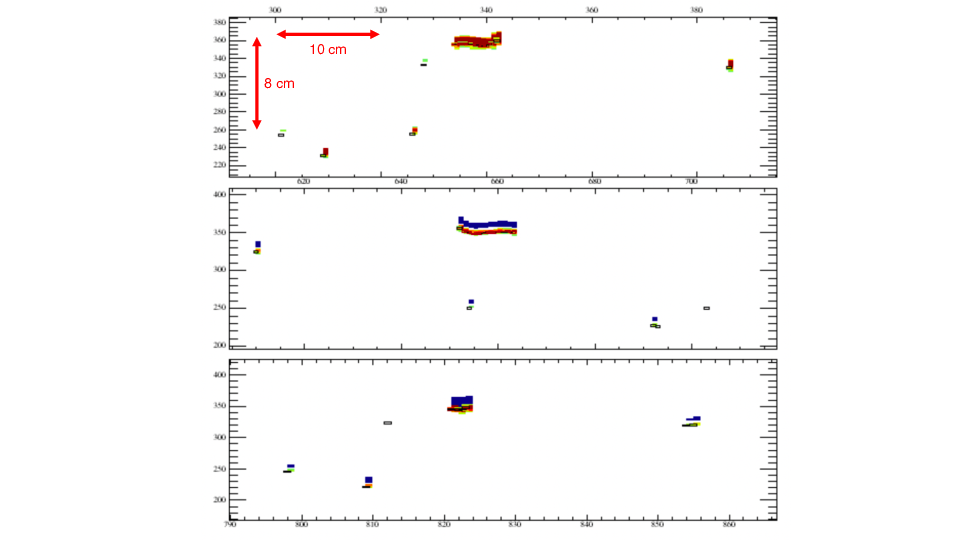
\includegraphics[width=\textwidth]{graphics/IntroFigures/nueCC_20-25MeV_event25_2.png} %\hskip 1 in
%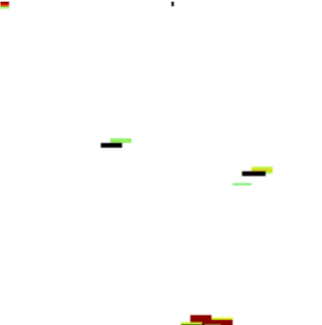
\includegraphics[height=0.5\textwidth]{graphics/IntroFigures/Fig_10b_Picture4.png}
\end{dunefigure}



Supernova candidates pose a unique problem for data acquisition and reconstruction.  \dword{snb} physics in DUNE is discussed in some detail in the far detector \dword{tdr}\cite{ Abi:2020evt}, reference \cite{Cuesta:2020dy} and a dedicated paper \cite{DUNE:2020zfm} and only summarized here. 

\dword{dune} is uniquely sensitive to $\nu_e$ through the reaction $\nu_e + Ar \rightarrow e^- + K*$ which leaves an electron trajectory that can be used to estimate the direction of the supernova.  Figure \ref{fig:SNrates} shows the expected neutrino interaction rates from supernovae as a function of their distance.
%The number of neutrino interactions actually detected depends on the physics of the supernova burst, oscillation physics and the minimum energy threshold achievable in the DUNE \dword{tpc} in the presencen of radiological backgrounds.

A classic core-collapse supernova 10\,kpc away would be expected to yield around 3,000  \dword{cc} electron neutrino interactions across four detector modules. \dword{snb} candidates will be quite different from beam interactions, having small interactions with energies in the 5-30\,MeV range spread across the full volume of the detector modules over many seconds, in contrast to the localized, coincident,  500-10,000\,MeV signature of beam neutrino interactions. These differences impose interesting requirements on the \dword{daq} and computing models for the experiment.  


\dword{snb} physics and its influence on neutrino emission are not fully understood and will result in significant modulations of the event rates for different neutrino types  over the few tens of seconds of the burst.  DUNE's fine-grained tracking should allow significant pointing power with the most optimistic scenario of four modules and high electron neutrino fraction yielding pointing resolutions of less than 5 degrees.   Figure \ref{SNe} illustrates simulated signatures of \dword{snb} neutrino interactions in the far detector. The ability to produce a reasonably fast pointing signal would be extremely valuable to optical astronomers doing followup, especially if the supernova were in a region where dust masks the primary optical signal.   The need to be alert to supernovae and to quickly transfer and process the data imposes significant requirements on triggering, data transfer and reconstruction beyond those imposed by the %anne more regular 
beam-based oscillation physics. 
%For example, a compressed \dword{snb} readout of all four modules will be of order 184\,TB in size and take a minimum of four hrs to transfer over a 100\,Gbs network,  and then take of order 130,000 CPU-hrs for signal processing at present speeds.  If processing takes the same time as transfer, a peak of 30,000 cores would be needed. 

%%\subsection{Supernova \hideme{Schellman/Kirby - needed}}
%\todo{should this move to the introduction} 
%\cite{Cuesta:2020dy} % CHEP talk

%As noted in the introduction, the  \dword{dune} far detectors are sensitive to core-collapse supernovae.  References \cite{DUNE:2020zfm, Cuesta:2020dy} describe recent simulation studies of DUNE's sensitivity to core-collapse supernova signals in our Galaxy.

% \dword{dune} is uniquely sensitive to $\nu_e$ through the reaction $\nu_e + Ar \rightarrow e^- + K*$ which leaves an electron trajectory that can be used to estimate the direction of the supernova.  Figure \ref{fig:SNrates} shows the expected neutrino interaction rates from supernovae as a function of their distance.
% The number of neutrino interactions actually detected depends on the physics of the supernova burst, oscillation physics and the minimum energy threshold achievable in the DUNE \dword{tpc} in the presencen of radiological backgrounds. 

The \dword{tpc} and \dword{pd} detectors produce several signals of increasing precision.  First, scintillation light is detected by the photon detectors, yielding fast triggering information.  Trigger primitives based on a subset of the \dword{lartpc} information can also be searched for supernova signatures.  Finally a full detector readout can be mined for information across the full spatial and energy range of the detector over a period of up to 100 s.  Trigger information from the \dwords{pds} and trigger primitives is available quickly and would lead to a completed long readout of the full detector system in the event that a candidate \dword{snb} is detected. 

In reference \cite{DUNE:2020zfm} the performance and efficiency of fast triggering on scintillation light and \dword{tpc} hits are investigated.  Radiological and noise backgrounds are required to produce less than 1 false trigger/month. Both \dword{pd} and \dword{tpc} based triggers are sensitive relatively low numbers of interactions ($\sim10-25$) at acceptable background rates, yielding expected sensitivities out to the Large Magellanic cloud.

Once the trigger system has identified a potential \dword{snb} signal  the \dword{daq} then records information for 100 s, yielding 130 TB of uncompressed information for a \dword{hd} module and 170 TB for a \dword{vd} module.  These data must then be transferred offsite for processing with the full algorithms. 

%Information from \dword{dune} comes at three levels.  First,  fast identification of a supernova candidate, based on raw \dwprd{toc} and \dword{pd}  information, second, first-pass pattern recognition on a subset of the data which could provide pointing information on a time scale of seconds to hours and finally, full reconstruction of all information available down to the detector threshold in the few MeV range to exact maximal physics information from these extremely rare events. %Optimal use of this information requires 



Moving  300 TB (assuming the first 2 modules) of uncompressed data   from \dword{surf} to processing centers will require, at minimum, 6-7 hours with the planned 100Gbs network link.  This can be accelerated by implementing onboard data compression and may require upgrades to the network when the projected third and fourth modules come online.  The need to store up to 300 TB of data from a supernova candidate while also continuing normal data taking drives the size of local disk buffers at \dword{surf} and presumably required similar reserved or rapidly-preemptable space at the centers where the data would be processed. Our \dword{protodune} experience indicates that reconstruction of \dword{lartpc} data takes between 1 and 3 sec/MB of raw data on present day computing resources.  It will thus take of order 12,000-40,000 cores to perform a preliminary reconstruction the data as fast as it comes in. In principle, a significant fraction of the neutrino data could be processed  in the 2-4 hours before a supernova becomes visible at optical frequencies.

Other neutrino detectors worldwide will also be able to provide fast information but the \dword{dune} information will be unique in its sensitivity to electron neutrinos. 




%\todo{more test on the network and processing challenges}



\section{Near Detector \hideme{Junk/Muether - needs update}}

High-precision oscillation physics requires a \dword{nd} system to allow measurement of the original neutrino flux and %anne improved understanding of neutrino interaction physics. 
to provide improved understanding of neutrino interaction physics. 
The DUNE  collaboration is proposing a suite of near detectors optimized for these two goals. 
 
 The \dword{nd}  will be located in an enclosure on the \dword{fnal} site 574\,meters from the target %anne and will be exposed to the DUNE 
 in the path of the neutrino beam.    Interaction rates per spill (at 0.83\,Hz) are expected to be very large, with 40-60 interactions per spill, including muons originating from interactions in material upstream of the fiducial volumes. Figure~\ref{beamline} shows the beamline and location of the \dword{nd} on the \dword{fnal} site. There are three major subdetectors:
 A pixel readout %anne liquid argon detector
 \dword{lartpc}, \dword{ndlar}, is  the most upstream of the three subdetectors shown in Figure~\ref{nd}, where the beam propagates  from right to left. Immediately downstream of \dword{ndlar} is the gaseous liquid argon detector, \dword{ndgar}, which serves %anne \dword{ndlar} 
 as  a muon spectrometer and allows more detailed study of neutrino interactions. %anne that occur within its gas volume. 
 Beyond \dword{ndgar}, is the \dword{sand} component of the \dword{nd} that acts as a beam monitor. %Figure \ref{nd} shows the three \dword{nd} subdetectors in the near enclosure. 
Note that while the \dword{nd} will have the same DAQ timing window flexibility as the \dword{fd}, it is not foreseen that \dword{nd} physics goals will required the utilization of varied time windows for trigger records as compared with the \dword{fd}. %Kirby


 \begin{dunefigure}
[The neutrino beamline on the Fermilab site]
{beamline} % Anne: label should have fig:
{The neutrino beamline on the \dword{fnal} site. The near detectors will be situated 574\,m from the target and 62\,m below grade.}
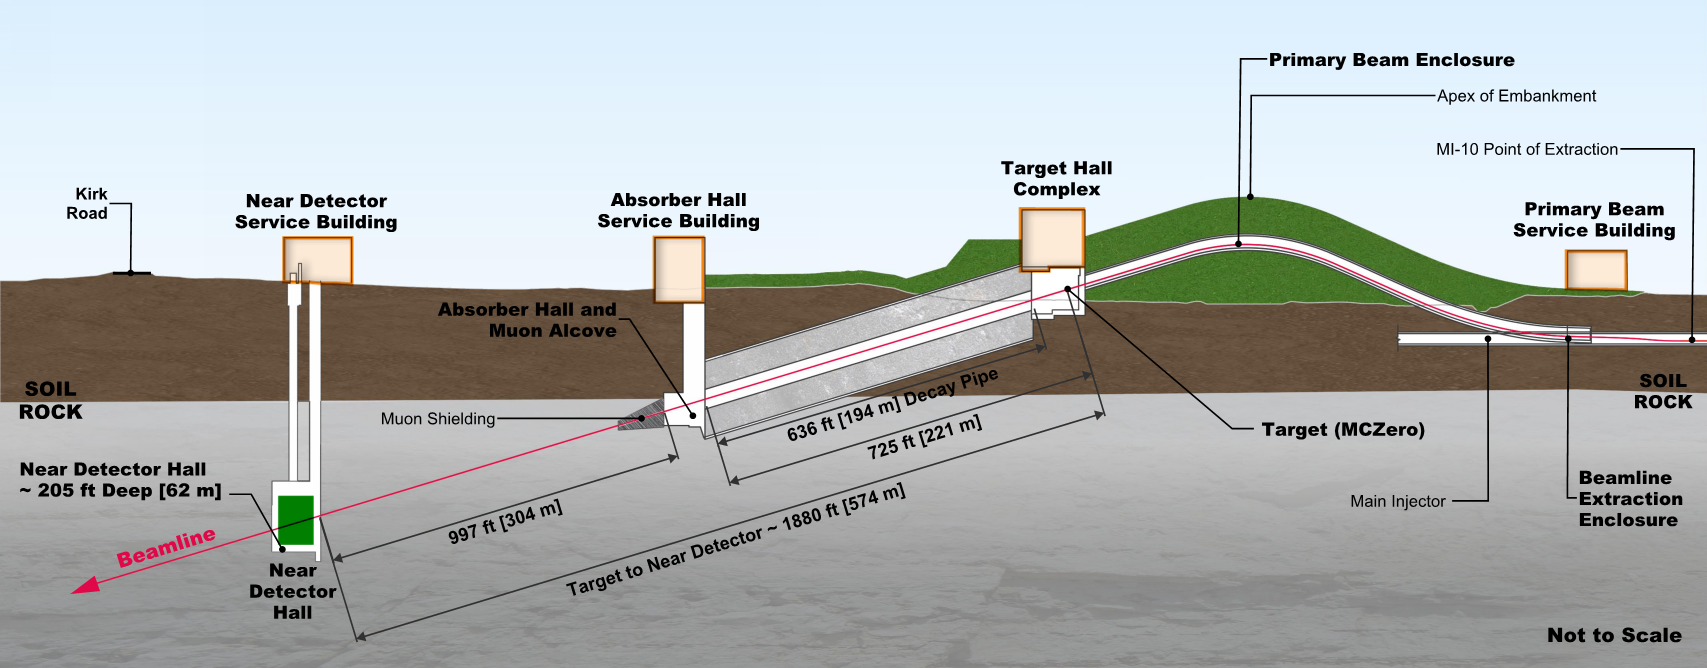
\includegraphics[height=0.3\textwidth]{graphics/IntroFigures/beamline-sideview.png}
\end{dunefigure}

 
 \begin{dunefigure}
[The ND systems in an on-axis configuration]
{nd}
{The \dword{nd} systems in an on-axis configuration.  The beam enters from the lower right in this view. The \dword{sand} scintillating beam monitor remains at beam center while the pixel %anne ND-LAr TPC detector 
\dword{ndlar} and gaseous \dword{ndgar} \dword{tpc} detectors can be moved off-axis to make detailed studies of the neutrino flux at multiple angles.}
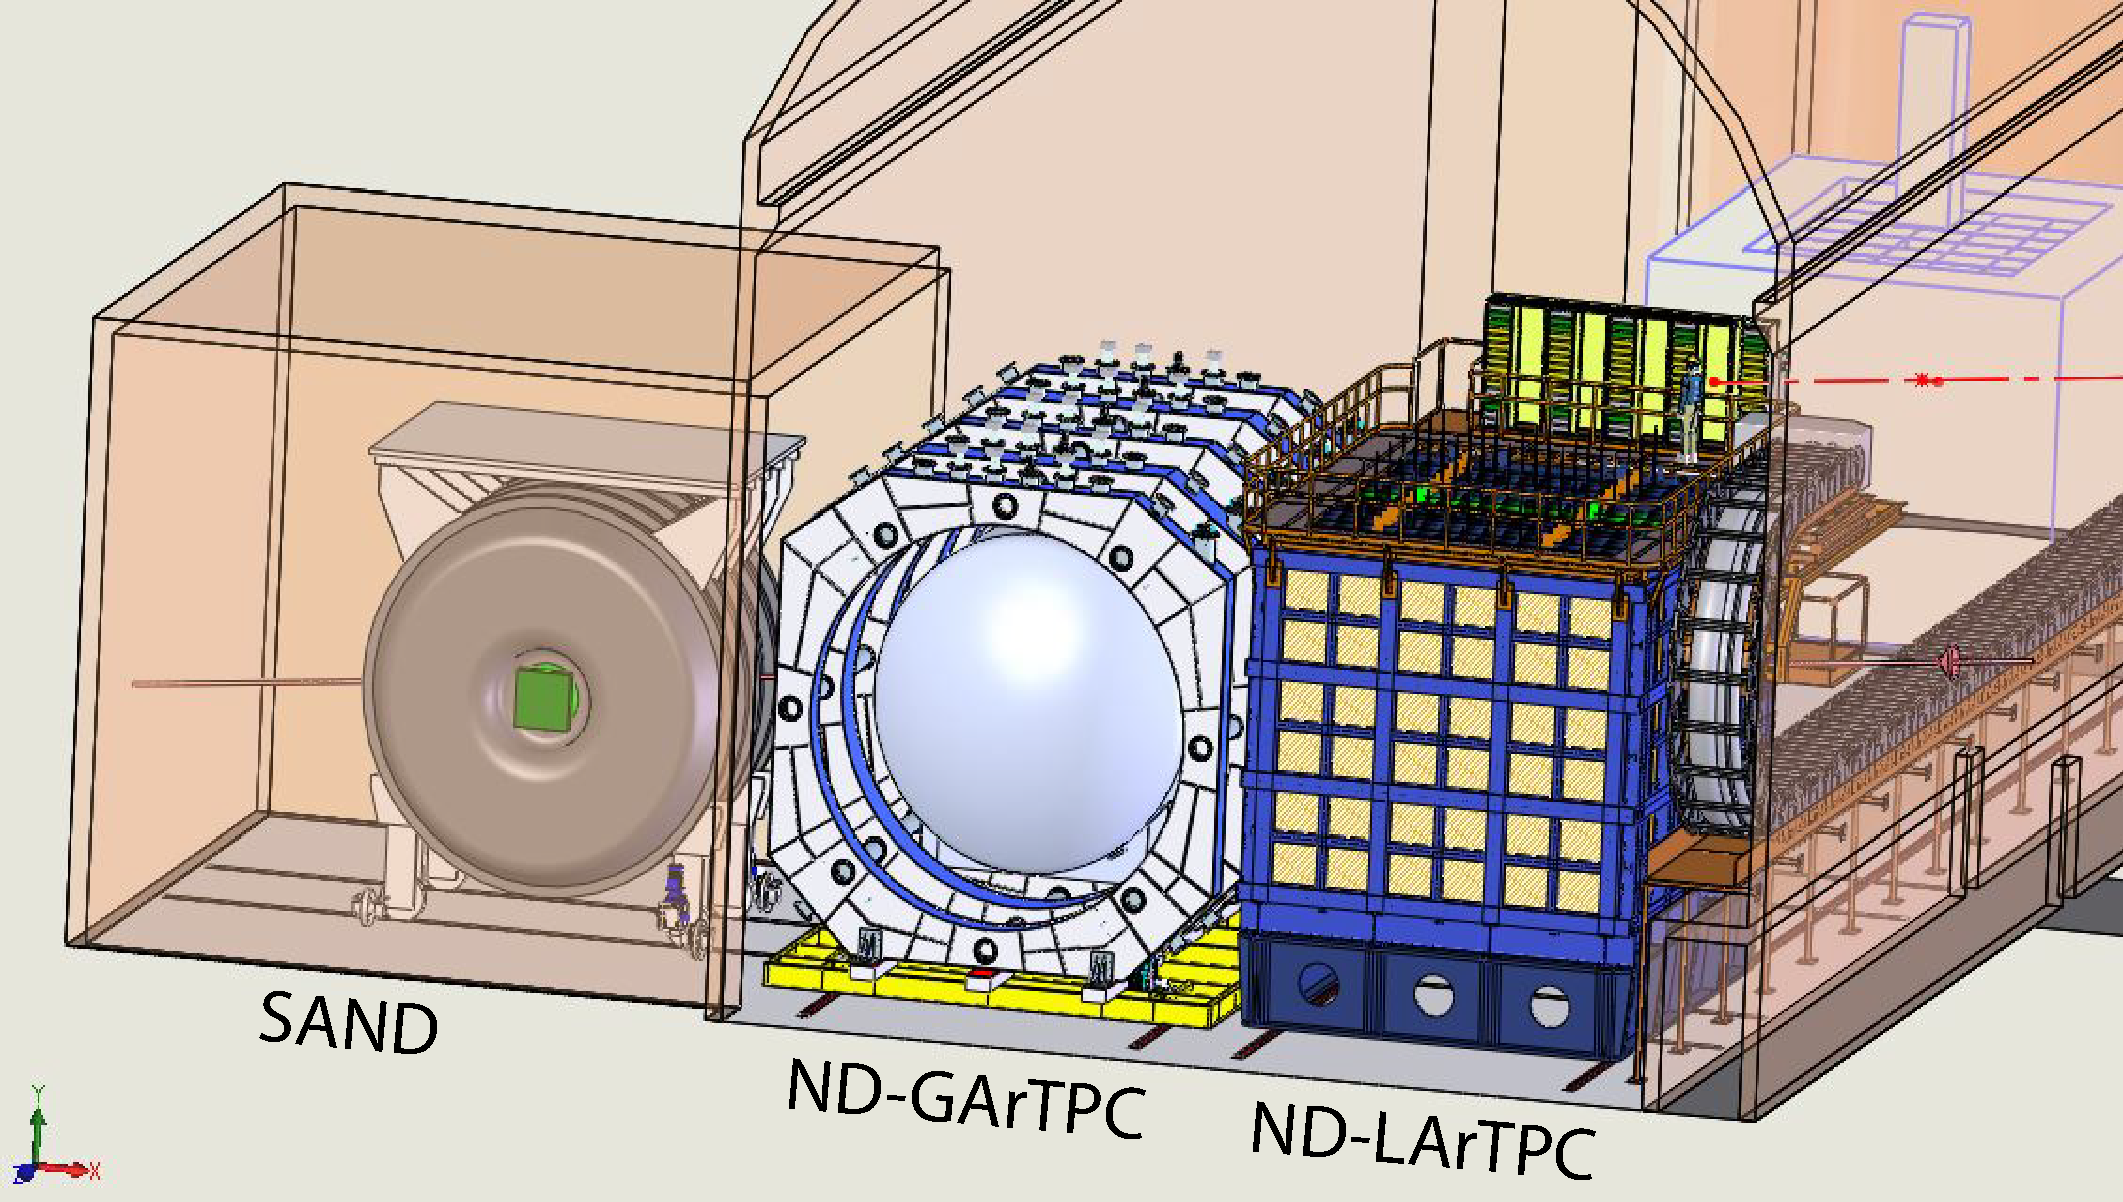
\includegraphics[height=0.5\textwidth]{graphics/IntroFigures/All3Detectors.pdf}
\end{dunefigure}

 \subsection{Pixel \dshort{lartpc} - \dshort{ndlar} \hideme{Muether - draft}}
 
 As the target material in the %anneDeep Underground Neutrino Experiment (DUNE) 
 far detector is \dword{lar}, optimal cancellation of systematic uncertainties between the near and far detectors requires that the near detector include a  \dword{lar} component to match the \dword{fd}.  However, at the intense neutrino flux and high event rate in the \dword{nd} region, occupancies will be too high to allow the \twod readout provided by conventional wire planes. A new \dword{arcube}  technology has been developed that allows pixelized charge readout  and provides unambiguous \threed imaging of  particle interactions.  The \dword{ndlar} component of the \dword{nd} is made up of a configuration of \dword{arcube}  \dwords{lartpc}  large enough to provide the required hadronic shower containment and statistics.  %The 5 m (along beam)×7 m (horizontal,  transverse to beam)×3 m (height), 67 t fiducial mass, of ND-LAr are optimized primarily for  hadronic containment under the assumption that ND-GAr will measure the sign and momentum  of downstream exiting muons. Figure 2.2 shows the arrangement of modules in the crystat for  ND-LAr.  Section 2.2 gives a discussion of the physics consideration
 
 The pixel \dword{lar} detector will have 12~million $3 \times 3$\,mm$^2$ pixel channels and $\sim$4200 \dword{pd} channels.  The \dword{lartpc} will read out only pulse times and integrals, in contrast to the far detector which reads out every time slice.  The \dwords{pd} will, however, read out complete wave-forms.   A total of 3\,MB of uncompressed data is anticipated per spill from the \dword{tpc} with 5\,MB from the \dwords{pd} leading to an estimate of 144\,TB/year for uncompressed in-spill data. Calibrations and cosmic ray data increase that data volume by around 20\%.

% For calibrations, 300 runs are assumed to be taken per year, each generating 10~GB of data, for the TPC, and a similar set of runs for the photon detectors.  These runs include pulser runs, laser runs, radioactive source runs, or other special-condition runs that require taking data outside of the regular spills.  Since they are not tied to the spill timing structure, they can be collected at higher trigger rates and take less time.

% In addition to the beam data, cosmic rays will contribute to the data volume.  For the \dword{ndlar} geometry in the ND hall, the anticipated rate
% of cosmic rays is 100~Hz.  If all cosmic ray data were collected, the data volume would be approximately 1~MB/sec.  The scenario considered here is to
% collect one spill's worth of cosmic ray data for every ten beam spills, for a data volume of 6.3 TB per year.  While the activity on the cosmic-ray triggers is expected to be much less than that on a beam spill, it is assumed that the cosmic-ray triggering will continue even when the beam is off.

% The TPC-only out-of-spill and calibration numbers have been scaled by 8/3 to account for photon detector data, assuming full waveform readout in these samples, yielding the same ratio as in-spill data and the same compression. 

\subsection{Near Detector \dshort{gartpc} \hideme{Muether - draft}}
\label{sec:comp-dataestimates-mpd}

The \dword{ndgar} is a magnetized detector system consisting of a high-pressure \dword{gartpc} surrounded by an \dword{ecal} and a muon system. The \dword{ndgar} measures the momentum and sign of charged particles exiting the \dword{ndlar}. In addition, for neutrino interactions occurring in the \dword{ndgar} itself, higher resolution and lower momentum thresholds can be achieved for charged particle tracks, leading to improved neutrino interaction models. This capability enables further constraints of systematic uncertainties for long-baseline neutrino  oscillation analyses.

The \dword{ndgar} is composed of 678,136 readout pads in the \dword{tpc}, and approximately 3~million channels in the \dword{ecal}.  Approximately one in five spills will generate an interaction in the \dword{gartpc}, but particles entering the gas from interactions in the \dword{ecal} will provide the bulk of the data volume.  The readout strategy will be similar to the \dword{lartpc}, with only time and integral recorded. A  data volume of 2\,MB of uncompressed data per spill is expected from the \dword{tpc}.  The calorimeter is expected to contribute approximately 1\,MB per spill of uncompressed data.

% For calibrations, 300 runs per year generating 10~GB of data per run are assumed for the TPC, and a similarly-sized set of calibration runs are assumed for the \dword{ecal}.  Cosmic rays are expected to be collected between spills and when the beam is off.

\subsection{Near Detector Day One Muon Spectrometer (TMS) \hideme{Muether - draft}}
\label{sec:comp-dataestimates-mpd}

The TMS, a low-cost low-risk detector, will operate for the early part of the DUNE running when beam intensities are at their lowest and DUNE is not systematics limited. The TMS is a magnetized steel range stack (similar to MINOS \cite{minosNIM}) between ND-LAr and SAND.  The purpose of the TMS is to measure the momentum of 1 - 5 GeV muons that exit ND-LAr by range with a momentum precision comparable to the Far Detector (taken to be 4\%). The steel will be magnetized to identify the charge of muons it detects with better than 98\% accuracy. These metrics are designed to ensure the DUNE physics program will function for the first 2-3 years of TMS operations with no degradation to physics output.

The TMS consist of 200 total layers of alternating steel and scintillator. The first 40 layers of steel are 1.5 cm thick. The rear 60 layers of steel are 4 cm thick. There is a 4 cm gap between each steel layer. The steel plates are magnetized in the geometry. The thin (thick) central steel is given a vertically oriented downward pointing field of 1.25 T (0.9 T), while the outer steel thin (thick) steel plates have their field pointing upwards with a strength of 1.5 T (1.0 T). The scintillator is implemented as a collection of 3.5~cm wide by 3~m tall by 1~cm thick vertical bars arranged into modules of 1.68 m wide. Four modules are placed side by side into a layer. These scintillator layers are replicated in the gap between steel layers.  

The TMS is placed 8.2 m downstream from the ND-LAr (center to center) and centered 2.51 m below the origin in $y$. 


\subsection{SAND \hideme{Muether - draft}}
\label{sec:comp-dataestimates-sand}
%The 3rd detector subsystem is the \dword{sand}, a scintillator based monitor, consists of a 3-D pixelated scintillator detector, an electromagnetic calorimeter and XXX

The \dword{sand} component of the \dword{nd}'s primary function is the primary beam flux monitor.   \dword{sand} consists of an active scintillator target \dword{3dst} followed by a tracking system immersed in a solenoidal superconducting magnet  and  a $4\pi$ electromagnetic calorimeter.

\dword{sand}'s \dword{3dst} calorimeter component is composed of 11,520,000 $1\times 1\times 1$~cm$^3$ scintillating cubes, read out by 153,600 fibers.  There are expected to be approximately 2,160 hits per spill with a total of 0.13\,MB of data per spill.  The  \dword{ecal}~\cite{Adinolfi:2002zx} uses 4,850 \dwords{pmt}, with an estimated 5,500 total hits per spill or 33\,kB of packed data per spill.   The data volume from \dword{sand} is 4.3\,TB/year with these assumptions.  The amount of data from out-of-spill cosmic rays is estimated to be 20\% of that of the in-spill data, or approximately 1\,TB.  The data volume from \dword{sand} is significantly smaller than that from the \dword{ndlar} and the \dword{ndgar} due to the relative sizes of the three-dimensional tracking volumes and the segmentation choices.



% Test using \dword{tms}

%\subsection{Simulation challenges}

\section{Relation of Physics Goals to Offline Computing Challenges \hideme{Schellman-draft}}

The DUNE physics program drives several detector characteristics that pose novel computing challenges.  While the overall data volumes are smaller than those routinely handled by the large \dword{lhc} experiments, the remote detector site and unique physics goals present novel computing challenges. 

\begin{description}
\item{\bf Fine segmentation needed for electron-photon discrimination: \\}   The primary goal of the DUNE long baseline experiment is measurement of $\nu_\mu\rightarrow\nu_e$ and $\nubar_\mu\rightarrow\nubar_e$
oscillation probabilities for GeV scale accelerator neutrinos.   These oscillation probabilities are intrinsically low and sensitive to backgrounds where the neutral current process  $\nu_\mu+A\rightarrow\nu_\mu+\gamma+X$
produces a photon that %anne fakes 
mimics an oscillation signal.  Fine detector segmentation is necessary to distinguish between these scenarios. Figure~\ref{fig:Argoneut} illustrates this capability. The need for sub-cm-level segmentation drives the technology choice of \dwords{lartpc} and %anne hence 
the number of channels.   
\item{\bf Low-energy thresholds for astrophysical neutrinos: \\}
Other important physics goals are the detection of astrophysical neutrinos from the sun, possible supernovae burst neutrinos, atmospheric cosmic rays and %physics beyond the standard model (BSM) 
\dword{bsm} signatures in the \dword{fd}.  Astrophysical neutrinos produce lower-energy signatures, in the 1-30\,MeV range. Extracting such signals, near the noise threshold of the detector and in the presence of radiological backgrounds, requires careful attention to signal processing and zero-suppression for the \dword{fd} \dword{tpc} and \dword{pd} wave forms.  The need to optimize the low-energy threshold drives our need to carefully record waveforms with minimal processing. 

\item{\bf Precise energy calibrations:\\}
An additional challenge in oscillation physics is the need for accurate energy calibration in order to fully %anne utilize 
exploit the energy spectrum of the reconstructed neutrinos to further constrain oscillation parameters. While \dword{lar} detectors have a reputation for stability, the large volumes, complex \efield configurations, liquid motion, and potential variations in electron lifetime and drift velocity make it necessary to have large calibration data samples that span the full \dword{fd} detector volume.  Large cosmic ray and artificial calibration samples will dominate the total data volumes from the \dword{fd}. 

\item{\bf Supernovae:\\}A %anne supernova 
\dfirst{snb} candidate will generate 115\,TB of (uncompressed) data per module. This means tens of thousands of data files produced over a 100\,s period. These data must be recorded at low energy threshold due to the expected interaction energy range, but must also be analyzed quickly and coherently in order to measure the time evolution of neutrino emissions, which carries invaluable information about the supernova process itself. In addition, if \dword{dune} can quickly analyze \dword{cc} interactions, we can provide pointing information to telescopes for optical followup.  %anne Supernova 
\dword{snb} physics drives the need for fast data transmission from the \dword{fd} to computing facilities and for robust tracking of data movement so that a full picture of the supernova interaction can be reassembled after signal processing.
As well, the drastically different time scale of \dword{snb} physics places requirements on the software framework. %Kirby

\item{\bf \dword{nd} integration: \\}
While the \dword{fd} %detectors 
modules produce large data volumes, the detectors themselves are reasonably simple, consisting of a small number of technologies and large numbers of repeating components.  The \dword{nd} is much more complex. 

The \dword{nd} use case is similar to other fixed target experiments such as \dword{sbnd} at \dword{fnal} and \dword{compass} at \dword{cern}.  The main computing challenge for the \dword{nd} will be integration of a large number of disparate detector technologies into a coherent whole. Here careful attention to simulation, detector geometry and configuration, and code management will be the major challenges. 

\item{\bf Analysis and parameter extraction:\\}
\dword{dune} has over one thousand collaborators spread across four continents. Those collaborators will want to analyze our data over several decades. Fortunately, once reconstruction has been done, neutrino interaction samples are generally simpler than event records at colliders and should %anne be analyzable locally. 
allow researchers to analyze them at their local institutions. However, final parameter extraction  using large numbers of nuisance parameters remains a computationally intense problem and will require significant resources
and efficient utilization of \dword{hpc} to quickly achieve final results. 



\end{description}

\section{Summary of Challenges \hideme{Schellman-draft}}

DUNE offline computing faces four major challenges, some of which are unique to DUNE and others shared widely by \dword{hep} experiments.  

\begin{description}
\item{\bf Large memory footprints -}  DUNE events, with multiple data objects consisting of  thousands of channels with thousands of time samples   present formidable challenges for reconstruction on typical \dword{hep} processing systems. Efficient processing of DUNE data will require careful attention to data formats and, likely, substantial redesign of the processing framework to allow sequential processing of chunks of data.  Chapters~\ref{ch:appl} and~\ref{ch:fworks} describe the status of applications and frameworks. 

\item{\bf Storing and processing data on heterogeneous international  resources -} DUNE depends on the combined resources of the collaboration for large-scale storage and processing of data.   Tools for using shared resources ranging from small-scale clusters to dedicated \dword{hpc} systems need to be developed and maintained.   Fortunately, \dword{hep}, through the \dword{wlcg}, \dword{osg} and \dword{hsf}  has a well developed ecosystem of tools that allow reasonably transparent use of collaboration computing resources.  Chapters~\ref{ch:est}, \ref{ch:cm} and~\ref{ch:datamgmt} describe the data volumes, computing model and data management plans. 

\item{
\bf Machine learning - }  Use of machine learning techniques can greatly improve simulation, reconstruction and analysis of data. However, integration of \dword{ml} techniques into a software ecosystem of the size and complexity of a large \dword{hep} experiment requires substantial effort beyond the original demonstration.  How is the \dword{ml} trained?  What special data format or processing requirements are present? How is the algorithm versioned and preserved to ensure reproducibility?   Chapters~\ref{ch:appl} and~\ref{ch:codemgmt} discuss the applications and management.

\item{\bf Keeping it all going -}  %anne There are a 
A large suite of activities, %anne that are 
while not necessarily novel, %anne but 
still need to be done over the full lifetime of the experiment.  These include database design and operations, security updates, code management, documentation, training and user support.   For example, the \dword{nd} presents few novel computing challenges in memory or CPU use but is highly complex in terms of the number of detector systems that must be integrated. Another example is the continuing evolution of operating systems and security requirements.  These require constant modifications to working systems to maintain operations.  A third activity is database design and maintenance. Here the problem is largely sociological, getting the attention of busy people to do database design and then %anne population and use. 
populate and use the databases. This requires continual engagement with reluctant stakeholders. These issues are discussed throughout this document with special reference to databases, Chapter~\ref{ch:db}, authentication Chapter~\ref{ch:auth}, code management Chapter~\ref{ch:codemgmt} and training and documentation Chapter~\ref{ch:train}
\end{description}
A broad suite of use cases is discussed in Chapter~\ref{ch:use}.


%\hideme{\section{What is missing?}}

\end{document}

\cleardoublepage




\documentclass[../main-00.tex]{subfiles}
\begin{document}

\chapter{Data and Processing Volume Estimates \hideme{Schellman, Junk, Muether}}
\label{ch:est}
\fixme{Heidi: moved tables of numbers from intro to here.  Still needs better organization}
In this chapter we will describe the assumptions that go into a bottoms-up estimate of data volumes and describe possible methods of reducing the total volumes while retaining physics capabilities. 

\section{Introduction}

% \begin{dunetable}
% [Data Sizes and Rates]
%  {l |r r r }
%  {tab:volumes}
%  {Data sizes and rates for different processes in each far detector module.  Uncompressed data sizes are given. As readouts will be self-triggering an extended 5.4 ms readout window is used instead of the 3ms for the triggered \dword{pdsp} runs.  We assume beam uptime of 50\% and 100\% uptime for non-beam science. These numbers are derived from references \protect{\cite{bib:docdb16028}}and \protect{\cite{bib:docdb14983}}.}
% % 5
%  Process & Rate/module & \qquad size/instance &\qquad  size/module/year\\ \toprowrule
%  %
%  Beam event & 41/day & 6 GB&47 TB/year\\
%  Cosmic rays &4,500/day&  6 GB& 9.7 PB/year\\
%  Supernova trigger& 1/month& 115 TB& 1.4 PB/year\\
%  Calibrations&2/year&750 TB& 1.5 PB/year\\
%  %\toprowrule 
%  Total& & &12.9 PB/year\\
%  \end{dunetable}




%  \subsection{Supernova candidates}


%  \begin{figure}
%  \begin{center}
%  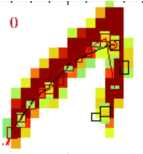
\includegraphics[height=0.3\textwidth]{graphics/IntroFigures/Fig_10a_Picture3.png} \hskip 1 in
% 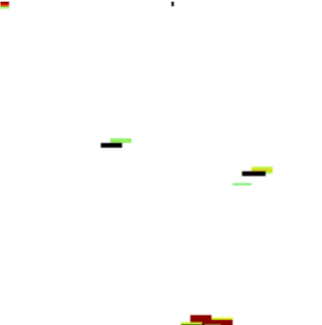
\includegraphics[height=0.5\textwidth]{graphics/IntroFigures/Fig_10b_Picture4.png}
%  \caption{Left) a charged current interaction of a 30 MeV energy electron neutrino in the DUNE Far Detector.  Right) a neutral current excitation and de-excitation of an Ar nucleus by a  10 MeV neutrino.}
%  \label{blips}
%  \end{center}
%  \end{figure}


% Supernova candidates pose a unique problem for data acquisition and reconstruction.  Supernova physics in DUNE is discussed in some detail in the \dword{tdr}\cite{ Abi:2020evt} and only summarized here. A classic core-collapse supernova 10 kpc away would be expected to yield around 3,000  charged-current electron neutrino interactions across 4 detector modules.  The oscillation physics is not fully understand and can result in significant modulations of the event rates for different neutrino types  over the few tens of seconds of the burst.  DUNE's fine-grained tracking should allow significant pointing power with the most optimistic scenario of four modules and high electron neutrino fraction yielding pointing resolutions of less than 5 degrees.   Figure \ref{blips} illustrates simulated signatures of supernova neutrino interactions in the far detector. The ability to produce a reasonably fast pointing signal would be extremely valuable to optical astronomers doing followup, especially if a supernova was in a region where dust masks the primary optical signal.   The need to be alert to supernovae and to quickly transfer and process the data imposes significant requirements on triggering, data transfer and reconstruction beyond those imposed by the more regular beam-based oscillation physics.   For example, a compressed supernova readout of all four modules will be of order 184 TB in size and take a minimum of 4 hrs to transfer over a 100 Gbs network,  and then take of order 130,000 CPU-hrs for signal processing at present speeds.  If processing takes the same time as transfer, a peak of 30,000 cores would be needed. 


% \fixme{Move or copy to the data volumes section}
% \begin{dunetable}
% [Useful FD Data Quantities]
% {|l  l |c       | l |}
% {tab:exec-comp-bigpicture-es}
% {Useful quantities for computing estimates for \dword{sp}
% readout. For  sparse \dword{fd} events, the pattern recognition phase, which scales with occupancy is expected to be substantially faster than the signal processing phase which scales with detector size.  }%
% Quantity&&\qquad Value \qquad&Explanation\qquad \qquad\\
% \toprowrule
% {\bf Far Detector Beam:}&&&\\ 
% &Single APA readout &41.5 MB& Uncompressed 5.4 ms\\ 
% &Single APA readout &16.6 MB& $\times 2.5$ compression\\
% &APAs per module& 150&\\
% &Full module readout &6.22  GB& Uncompressed 5.4 ms\\ 
% &Beam rep. rate&0.83 Hz&Untriggered\\  
% Signal processing &CPU time/APA&40 sec&from MC/ProtoDUNE\\  
% Signal processing &CPU time/input MB& 2.5 sec/MB& compressed input\\
% &Memory footprint/APA&0.5-1 GB&ProtoDUNE experience\\  
% \toprowrule
% {\bf Supernova:}&&&\\
% &Single channel readout &300 MB& Uncompressed 100 s\\  
% &Four module readout& 460 TB& Uncompressed 100 s\\  
% &Trigger rate&1  per month&(assumption)\\
% \end{dunetable}


% \dword{dune} requires a global software and computing effort to store, catalog, reconstruct, calibrate and analyze approximately 30 PB of data/year from  multiple \dword{lartpc} detectors containing 17 kT of liquid each,  a larger scale than any previous neutrino experiment. Single event sizes are expected to range from 200 MB for the existing \dword{protodune} experiments running at \dword{cern}, to 6 GB for a far detector module, to 460 TB for a full readout of a 100 s supernova candidate across 4 modules. Full sensitivity to neutrino oscillations, supernovae neutrinos,  and beyond the standard model phenomena  require precise energy calibration and energy thresholds in the few MeV range, which present significant challenges for signal processing.  In addition to the general distributed computing issues that are common to large \dword{hep} experiments, the very large event sizes present  \dword{dune} with a unique computing challenge.  \dword{dune} intends to benefit from previous experience and will contribute to ongoing improvements in general \dword{hep} computing infrastructure, working in collaboration with the \dword{osg}, the \dword{wlcg} , and the \dword{hep} Software Foundation among others.  However, the unique nature of    \dword{dune} events will require dedicated effort to adapt and integrate   \dword{dune}-specific solutions to achieve the physics goals of the experiment.

%\subsection{Near Detectors}
% \subsection{Near Detectors}

% High precision oscillation physics requires a near detector system to allow measurement of the original neutrino flux and improved understanding of neutrino interaction physics.  The DUNE  collaboration is proposing a suite of near detectors optimized for these two goals. 
 
%  The near detectors will be located in an enclosure on the Fermilab site 574 meters from the target and will be exposed to the DUNE neutrino beam.    Interaction rates per spill (at 0.83 Hz) are expected to be very large, with 40-60 interactions per spill, including muons originating from interactions in material upstream of the fiducial volumes. Figure \ref{beamline} shows the beamline and location of the near detectors on the Fermilab site. There are three major subsystems:
%  A pixel readout liquid argon detector, \dword{ndlar}, is  the most upstream of the three sub-detectors shown in Figure \ref{nd}, where the beam propagates  from right to left. Immediately downstream of \dword{ndlar} is the gaseous liquid argon detector, \dword{ndgar}, which serves \dword{ndlar} as  a muon spectrometer and allows more detailed study of neutrino interactions that occur within its gas volume. Beyond \dword{ndgar}, is the \dword{sand} component of the ND that acts as a beam monitor. %Figure \ref{nd} shows the three \dword{nd} subdetectors in the near enclosure. 
 
%  \begin{figure}[ht]
%      \centering
%      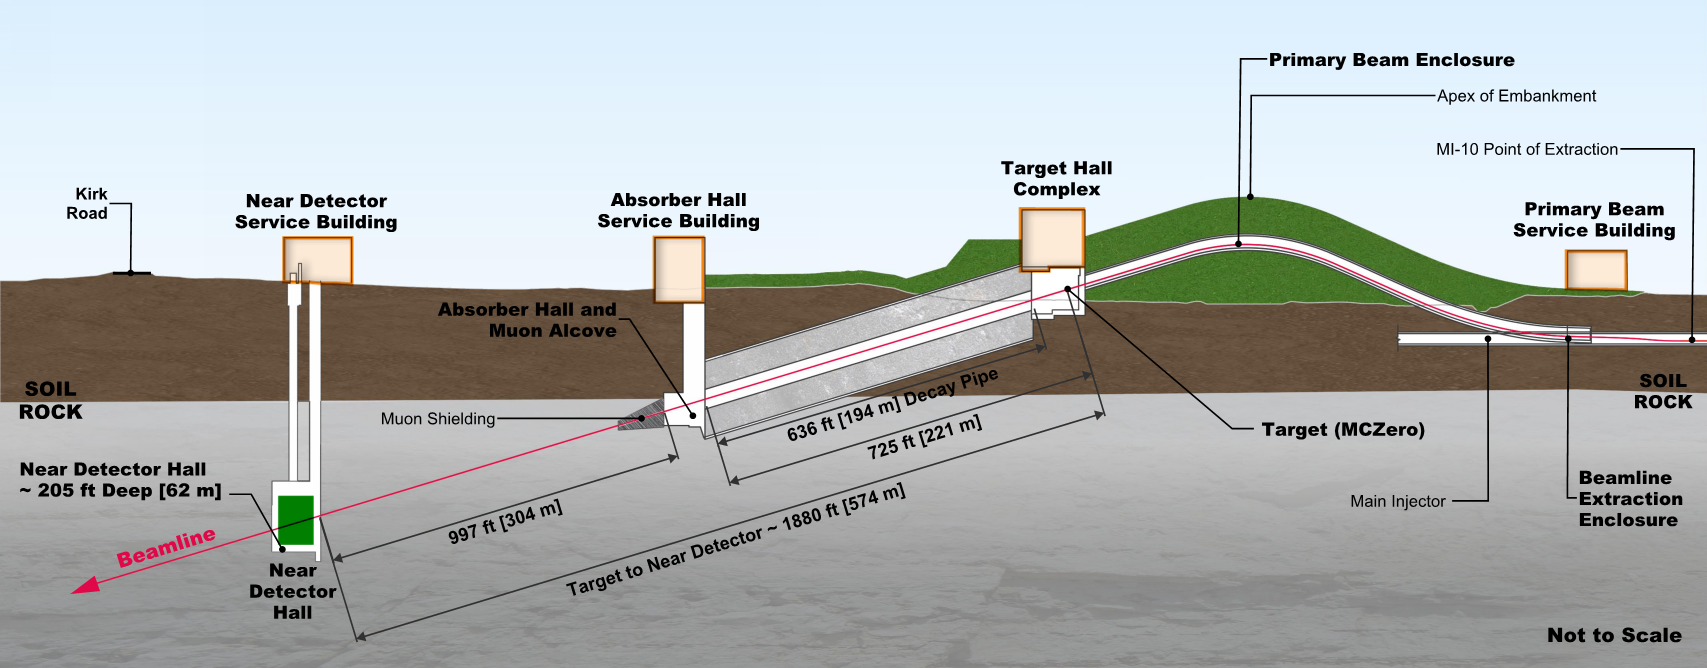
\includegraphics[height=0.3\textwidth]{graphics/IntroFigures/beamline-sideview.png}
%      \caption{The LBNF neutrino beamline on the Fermilab site. The near detectors will be situated 574 m from the target and 62 m below grade.}
%      \label{beamline}
%  \end{figure}
 
%  \begin{figure}[ht]
%      \centering
%      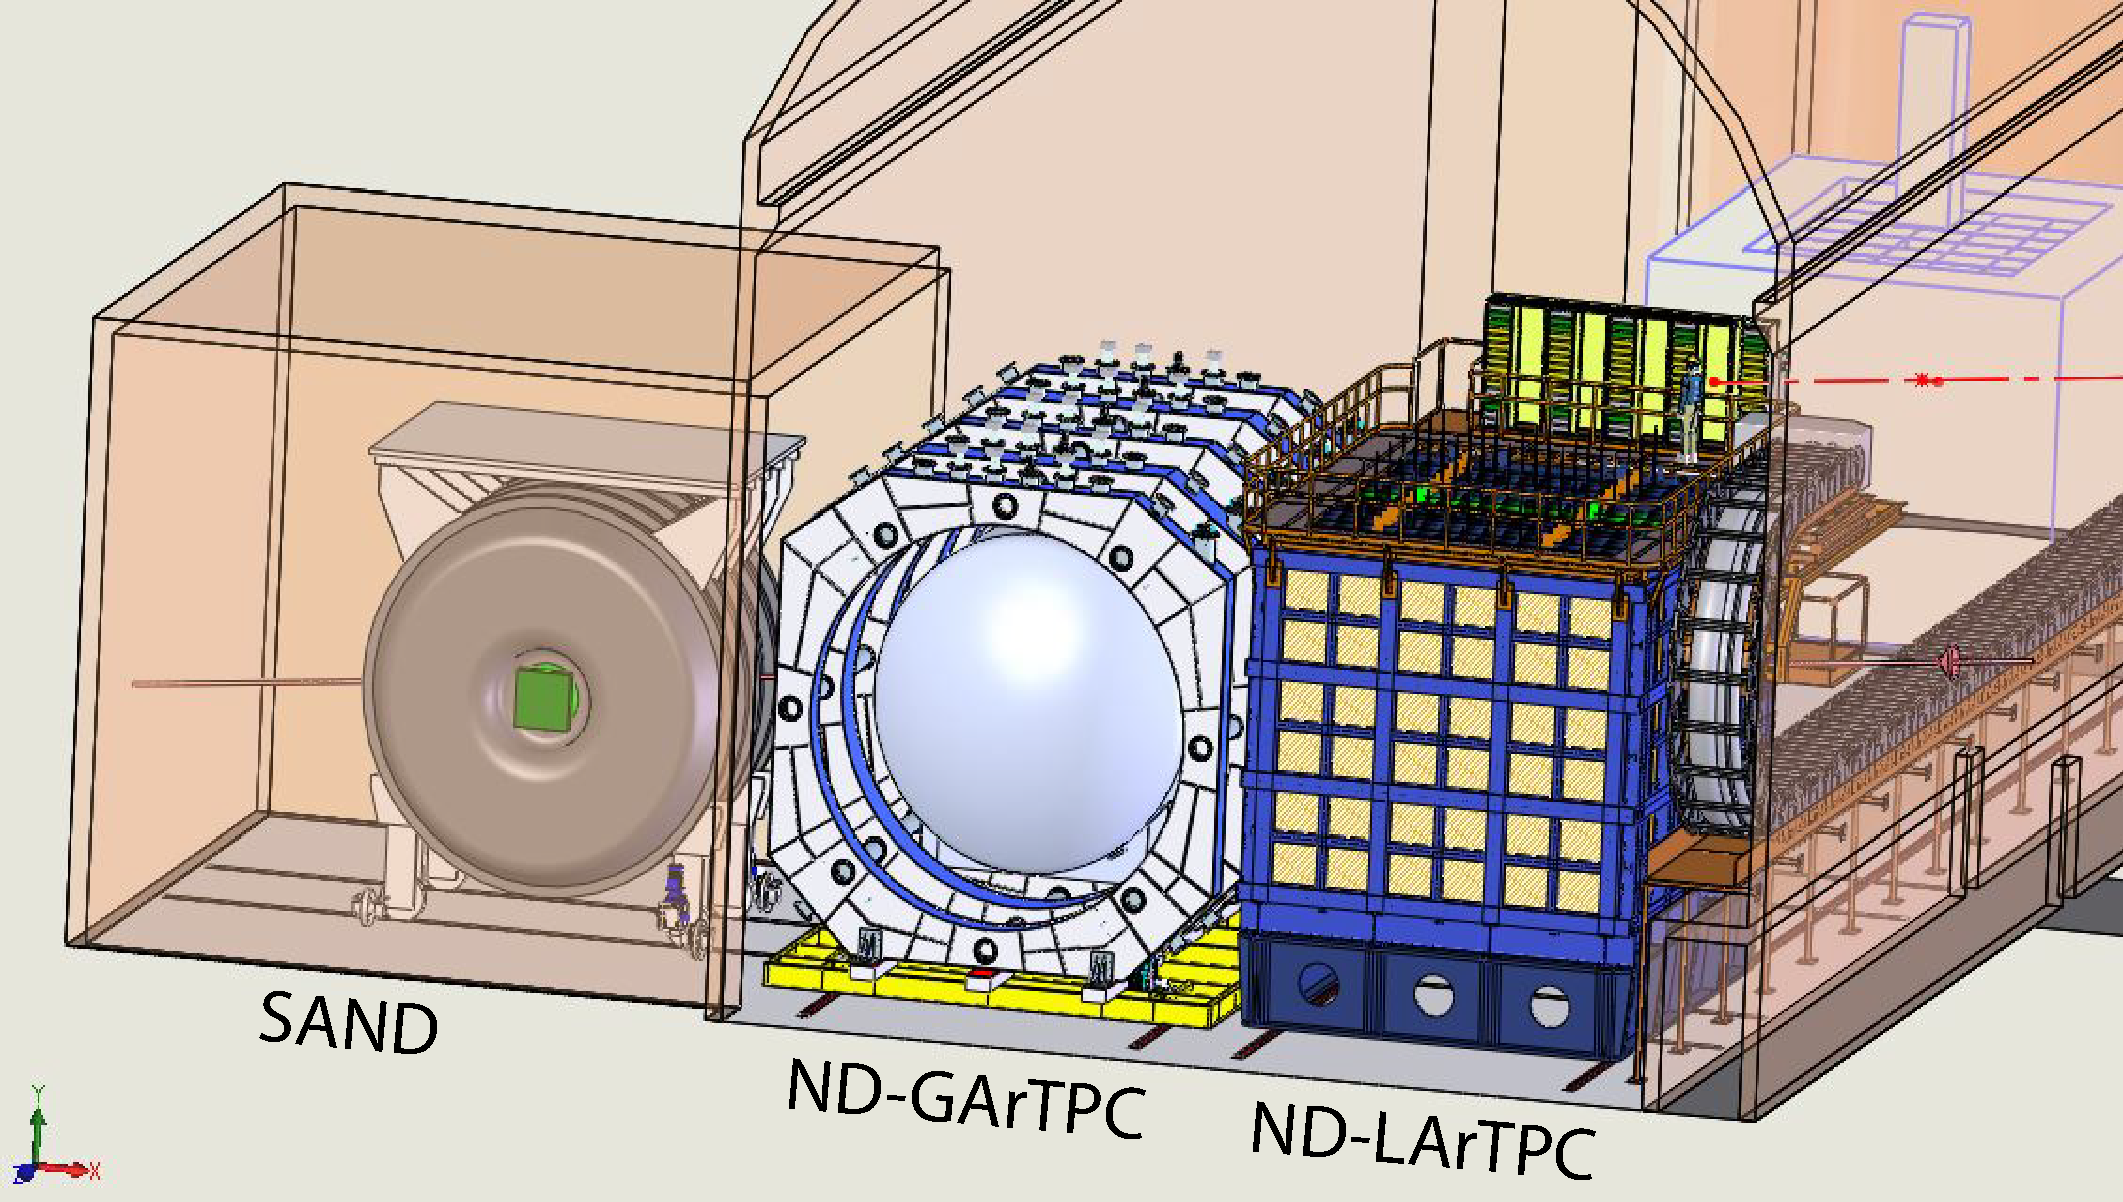
\includegraphics[height=0.5\textwidth]{graphics/IntroFigures/All3Detectors.pdf}
%      \caption{The near detector systems in an on-axis configuration.  The beam enters from the lower right in this view. The \dword{sand} scintillating beam monitor remains at beam center while the pixel ND-LAr TPC detector and gaseous ND-GAr TPC detectors can be moved off-axis to make detailed studies of the neutrino flux at multiple angles.  }
%      \label{nd}
%  \end{figure}
 
%  \subsubsection{pixel LArTPC - ND-Lar}
 
%  As the target material in the Deep Underground Neutrino Experiment (DUNE) far detectors is liquid argon, optimal cancellation of systematic uncertainties between the near and far detectors requires that the near detector include a liquid argon component to match the \dword{fd}.  However, at the intense neutrino flux and high event rate in the ND region, occupancies will be too high to allow the 2-D readout provided by conventional wire planes. A new ArgonCube  technology has been developed that allows pixelized charge readout  and provides unambiguous 3D imaging of  particle interactions.  The ND-LAr component of the DUNE ND is made up of a configuration of ArgonCube LArTPCs  large enough to provide the required hadronic shower containment and statistics.  %The 5 m (along beam)×7 m (horizontal,  transverse to beam)×3 m (height), 67 t fiducial mass, of ND-LAr are optimized primarily for  hadronic containment under the assumption that ND-GAr will measure the sign and momentum  of downstream exiting muons. Figure 2.2 shows the arrangement of modules in the crystat for  ND-LAr.  Section 2.2 gives a discussion of the physics consideration
 
%  The pixel liquid argon detector will have 12~million $3\times 3$~mm$^2$ pixel channels and $\sim$4200~photon detector channels.  The LArTPC will read out only pulse times and integrals, in contrast to the far detector which reads out every time slice.  The photon detectors will, however, read out complete wave-forms.   A total of 3~MB of uncompressed data is anticipated per spill from the TPC with 5-MB from the photon detectors leading to an estimate of 144 TB/year for uncompressed in-spill data. Calibrations and cosmic ray data increase that data volume by around 20\%.

% % For calibrations, 300 runs are assumed to be taken per year, each generating 10~GB of data, for the TPC, and a similar set of runs for the photon detectors.  These runs include pulser runs, laser runs, radioactive source runs, or other special-condition runs that require taking data outside of the regular spills.  Since they are not tied to the spill timing structure, they can be collected at higher trigger rates and take less time.

% % In addition to the beam data, cosmic rays will contribute to the data volume.  For the \dword{ndlar} geometry in the ND hall, the anticipated rate
% % of cosmic rays is 100~Hz.  If all cosmic ray data were collected, the data volume would be approximately 1~MB/sec.  The scenario considered here is to
% % collect one spill's worth of cosmic ray data for every ten beam spills, for a data volume of 6.3 TB per year.  While the activity on the cosmic-ray triggers is expected to be much less than that on a beam spill, it is assumed that the cosmic-ray triggering will continue even when the beam is off.

% % The TPC-only out-of-spill and calibration numbers have been scaled by 8/3 to account for photon detector data, assuming full waveform readout in these samples, yielding the same ratio as in-spill data and the same compression. 

% \subsubsection{Near Detector Gaseous Argon TPC}
% \label{sec:comp-dataestimates-mpd}

% The \dword{ndgar} is a magnetized detector system consisting of a high-pressure gaseous argon TPC  (HPgTPC) surrounded by an electromagnetic calorimeter (ECAL) and a muon system. The \dword{ndgar} measures the momentum and sign of charged particles exiting the ND-LAr. In addition, for neutrino interactions occurring in the \dword{ndgar} itself, higher resolution and lower momentum thresholds can be achieved for charged particle tracks, leading to improved neutrino interaction models. This capability enables further constraints of systematic uncertainties for long-baseline neutrino  oscillation analyses.

% The \dword{ndgar} is composed of 678,136 readout pads in the TPC, and approximately 3~million channels in the \dword{ecal}.  Approximately one in five spills will generate an interaction in the gas TPC, but particles entering the gas from interactions in the \dword{ecal} will provide the bulk of the data volume.  The readout strategy will be similar to the LArTPC, with only time and integral recorded. A  data volume of 2 MB of uncompressed data per spill is expected from the TPC.  The calorimeter is expected to contribute approximately 1~MB per spill of uncompressed data.

% % For calibrations, 300 runs per year generating 10~GB of data per run are assumed for the TPC, and a similarly-sized set of calibration runs are assumed for the \dword{ecal}.  Cosmic rays are expected to be collected between spills and when the beam is off.



% \subsubsection{SAND}
% \label{sec:comp-dataestimates-sand}
% %The 3rd detector subsystem is the \dword{sand}, a scintillator based monitor, consists of a 3-D pixelated scintillator detector, an electromagnetic calorimeter and XXX

% The \dword{sand} component of the near detector (ND)'s primary function is the primary beam flux monitor.   SAND consists of an active scintillator target \dword{3dst} followed by a tracking system immersed in a solenoidal superconducting magnet  and  a $4\pi$ electromagnetic calorimeter.

% \dword{sand}'s \dword{3dst} calorimeter component is composed of 11,520,000 $1\times 1\times 1$~cm$^3$ scintillating cubes, read out by 153,600 fibers.  There are expected to be approximately 2,160 hits per spill with a total of 0.13 MB of data per spill.  The  \dword{ecal}~\cite{Adinolfi:2002zx} uses 4,850 PMTs, with an estimated 5,500 total hits per spill or 33 kB of packed data per spill.   The data volume from SAND is 4.3 TB/year with these assumptions.  The amount of data from out-of-spill cosmic rays is estimated to be 20\% of that of the in-spill data, or approximately 1 TB.  The data volume from SAND is significantly smaller than that from the \dword{ndlar} and the \dword{ndgar} due to the relative sizes of the three-dimensional tracking volumes and the segmentation choices.

%\fixme{Move this to the Data volumes section}
%\subsubsection{CPU needs and simulation}

% Table \ref{tab:nd_data_volume_estimates} summarizes the expected data sizes from the near detector. Due to the much higher data density in the near detector, CPU times/beam spill are expected to be much higher and are estimated to be 300 CPU/sec/spill using current processors for $1.5\times 10^7$ spills/year. Simulated data samples will need to be an order of magnitude larger and thus require at least 10 times the CPU power.  This leads to a rough estimate of CPU needed of approximately 3,000 core-years/year.

% \begin{dunetable}[Near Detector Data Estimates]
% {l r}
% {tab:nd_data_volume_estimates}
% {Annual DUNE near detector data volume estimates.  No compression is assumed.}
% Type & Volume/year\\ \toprowrule
%     {\bf \dword{ndlar}}     &  \\
%     \quad\quad In-spill data & 144 TB \\
%     \quad\quad Out-of-spill cosmics & 16 TB\\
%     \quad\quad Calibration & 16 TB\\
%     \quad\quad Total & 176 TB \\\toprowrule
%     {\bf \dword{ndgar}}           & \\
%     \quad\quad In-spill data & 52 TB \\
%     \quad\quad Out-of-spill cosmics & 10 TB \\
%     \quad\quad Calibration & 6 TB\\
%     \quad\quad Total & 68 TB \\\toprowrule
%     {\bf \dword{sand}}        & \\
%         \quad\quad In-spill data & 4 TB\\
%     \quad\quad Out-of-spill cosmics & 1 TB\\
%     \quad\quad Calibration & 1 TB \\
%     \quad\quad Total & 6 TB \\\toprowrule
%     {\bf Total ND} & {\bf 250 TB}\\
% \end{dunetable}

% \begin{dunetable}
% [CPU estimates for Near Detector]
% {l r}
% {tab:NDCPUPerEvent}
% {Preliminary CPU estimates per event for the DUNE near detector components, in seconds.}
% Type&time/event\\ \toprowrule
%     {\bf LArTPC} &  \\
%     \quad\quad Monte Carlo gen+sim & 100 s \\
%     \quad\quad Reconstruction & 60 s\\\toprowrule
%   {\bf MPD} &  \\
%     \quad\quad Monte Carlo gen+sim & 100 s\\
%     \quad\quad Reconstruction & 12 s\\\toprowrule
%     {\bf SAND} & \\
%     \quad\quad Monte Carlo gen+sim & 100 s\\
%     \quad\quad Reconstruction & 10 s\\\toprowrule
% \end{dunetable}

% A Conceptual Design Report for the Near Detector systems is in preparation and the \dword{nd} computing efforts are being integrated with the existing far detector and protoDUNE efforts. 

%{\it borrowed from TDR to test bib/glossary/units}


% \section{Comments and Conclusions}
% This discussion has centered on the acquisition and fast processing of raw data from novel and extremely large liquid argon time projection chambers. Many other computing challenges lie ahead but were beyond the scope of this paper.  These include

% \begin{description}
% \item[{\bf Simulation:}] particle propagation in liquid argon is reasonably fast to simulate as there are not complicated volume boundaries to cross but simulating electron drift trajectories (and scintillation light trajectories) in a diffusive, electron absorbing, moving medium immersed in a non-uniform  electric field remains a challenging computational challenge. 
% \item[{\bf Near detectors:}] a suite of near detectors are needed to characterize the neutrino beam as it originates at Fermilab.  These detectors are still being developed but will introduce a large number of differing detector technologies.  While individual interactions are likely to be much smaller than readouts of the far detectors, the beam cycle is of order 1 Hz and each readout will contain multiple cosmic ray and beam interactions.
% \item[{\bf Data analysis:} ] The small (order 100) group of \dword{pdsp} and \dword{pddp} and \dword{dune} developers and analyzers have successfully analyzed the beam and cosmic ray data and performed simulations needed to produce the physics sections of the \dword{tdr}.  We expect analysis of the full experiment to involve many more individuals and much more data.  A campaign of training for new users and design of a suite of efficient analysis tools is needed.  We have initial prototypes based on NOvA and MicroBooNE analysis. 
% \end{description}

% Fortunately, \dword{dune} is able to take advantage of the huge and heroic developments in software and computing made for the Intensity Frontier and LHC experiments over the past decade.  We have demonstrated that, even with preliminary versions of our tools and algorithms, we can quickly reconstruct and analyze data from large liquid argon TPC's at full rate. We look forward to an exciting and fruitful next decade. 



% Test using \dword{tms}
%%%%%%%%%%%%%%%%%%%%%%%%%%%%%%%%
\section{Assumptions}
\label{sec:est:assume}  %% fix label according to section

\subsection{Raw data assumptions}
DUNE's detectors will produce information from a variety of technologies.  We anticipate that raw data volumes will be dominated by the digitized waveforms from liquid argon detectors and, to a lesser extent, photon detectors, in \dword{pd}, the \dword{fd} and the \dword{nd}.  
These raw data volumes can be reduced by the \dword{daq} system by several means.


\begin{itemize} 
\item triggered readout of particular time slices
\item triggered readout of particular geographic regions
\item lossless zero suppression
\item lossy zero suppression
\item hardware pattern recognition
\end{itemize}

Overall, we assume that the above methods can reduce data volumes from the hundreds of Exabytes that would be produced by continuous readout to a manageable 30 PB/year. 

\subsection{Derived data assumptions}


 \begin{dunetable}[Data Retention Policies]{llrrrr}{tab:est:retention}
{Retention policies by data tier}
Tier&Description&Tape copies& Lifetime &Disk Copies& Lifetime\\
Raw & Physics data& 2 & indefinitely & 1 & 1 year\\
Test & test and commissioning & 1 &6 months &1 & 6 months \\
Hits & reconstructed hits & 1 & 10 years & 1 & 1 month \\
Reco & pattern recognition &1 & 10 years & 2 & 2 years\\
\end{dunetable}

\section{ProtoDUNE}
\label{sec:est:ProtoDUNE}  

Our estimates  are largely based on our experience with the single and double-phase \dword{pd} detectors which ran at CERN in late 2018.  The \dword{pdsp} detector used \dword{hd} \dword{tpc} technology read out 6 \dwords{apa} and a mix of photon detectors while the first far detector module will have 150 \dwords{apa} and photon detectors based on the \dword{arapuca} technology.  Data rates and assumptions for protoDUNE have been documented in \href{docdb:20515}{https://docs.dunescience.org/cgi-bin/private/ShowDocument?docid=20515}.  Table \ref{tab:est:usefulpd} provides useful quantities for data volumes derived from the ProtoDUNE experience. 

 \begin{dunetable}[Useful quantities for computing far detector data volumes]{lrr}{tab:est:usefulpd}
{Useful quantities for computing estimates for \dword{sp}
readout.   }%\rowtitlestyle
Quantity&Value&Explanation\\
\toprowrule
%{\bf Far Detector Beam:}\\ \colhline
Number of channels/APA&2,560&\\
Readout time & 3 ms&\\
\# of time slices & 6000&\\
Single APA readout &23 MB& Uncompressed  estimate\\ \colhline
APAs & 6 &\\
Full detector readout &178 MB& Uncompressed real \\ \colhline
Full detector readout &71 MB& Compressed real \\ \colhline
Effective compression factor &2.5&\\ \colhline
Beam rep. rate&4.5 Hz&Average\\ \colhline
Hit reconstruction time CPU time/APA& 30 sec&from MC/ProtoDUNE\\ \colhline
Pattern recognition time CPU time event & 400 sec&from MC/ProtoDUNE\\ \colhline
Simulation time CPU time event & 2700 sec&from MC/ProtoDUNE\\ \colhline
Memory footprint/APA&0.5-1GB&ProtoDUNE experience\\ \colhline
\end{dunetable}

 

For example, uncompressed single phase data from ProtoDUNE-SP were observed to be around 178 MB in size, which is the amount expected for the number  of TPC channels read + a 20\% overhead for other detectors and headers.  Compressed SP data averages 71 MB, consistent with compression by a factor of 2.5.  

Dual phase data includes 2 CRPs for the 2019 run.  Observed data size without compression  was 110MB.  %Numbers for 2018 and 2019 have been 

For the far detector with APA's we assume 






[DUNE-doc-20515-v9]

\section{FD}
\label{sec:est:FD}  

For \dword{hd} far detector data volumes, we use our \dword{pdsp} experience and assume that raw data sizes and hit finding CPU times scale with the number of \dwords{apa} while pattern recognition and simulation times scale with the number of interactions. 

 \begin{dunetable}[Useful quantities for computing \dshort{hd} data volume
estimates]{lrr}{tab:est:usefulfd}
{Useful quantities for computing estimates for \dword{hd}
readout.}%\rowtitlestyle
Quantity&Value&Explanation\\
\toprowrule
{\bf Far Detector Beam:}\\ \colhline
Single APA readout &41.5 MB& Uncompressed 5.4 ms\\ \colhline
APAs per module& 150&\\
Compression factor &2.5 &\\
One full module readout &6.22  GB& Uncompressed 5.4 ms\\ \colhline
One full module readout &2.49  GB& Compressed 5.4 ms\\ \colhline
Beam rep. rate&\beamreprate&Untriggered\\ \colhline
Hit finding CPU time/APA&30 sec&from MC/ProtoDUNE\\ \colhline
Pattern recognition CPU time/event&400 sec&from MC/ProtoDUNE\\ \colhline
Simulation time CPU time event & 2700 sec&from MC/ProtoDUNE\\ \colhline
Memory footprint/APA&0.5-1GB&ProtoDUNE experience\\ \colhline
{\bf Supernova:}\\ \colhline
Single channel readout &300 MB& Uncompressed 100 s\\ \colhline
Four module readout& 460 TB& Uncompressed 100 s\\ \colhline
Four module readout& 184 TB& Compressed 100 s\\ \colhline
Trigger rate&1  per month&(assumption)\\
\end{dunetable}


DUNE \href{docdb:14893}{https://docs.dunescience.org/cgi-bin/private/ShowDocument?docid=14983} describes the expected event rates for various signatures in a \dword{hd} module.  These can be combined with the above numbers to provide  the integrated data estimates shown in table \ref{tab:est:hdrates}. 

 \begin{dunetable}
 [Horizontal Drift data volumes] {|l |r r r |}{tab:est:hdfdrates}
{Data sizes and rates for different processes in each horizontal drift detector module.  Uncompressed data sizes are given. As readouts will be self-triggering an extended 5.4 ms readout window is used instead of the 3ms for the triggered \dword{pdsp} runs.  We assume beam uptime of 50\% and 100\% uptime for non-beam science. These numbers are derived from references \cite{bib:docdb16028} and \cite{bib:docdb14983}.}
%\rowtitlestyle
%Quantity&Value&Explanation\\
%\toprowrule
%\begin{tabular}{|l |r r r |}
%\hline
Process & Rate/module & \qquad size/instance &\qquad  size/module/year\\
\hline
Beam event & 41/day & 6 GB&47 TB/year\\
Cosmic rays &4,500/day&  6 GB& 9.7 PB/year\\
Supernova trigger& 1/month& 115 TB& 1.4 PB/year\\
Calibrations&2/year&750 TB& 1.5 PB/year\\
\hline 
Total& & &12.9 PB/year\\
\end{dunetable}%



 Table~\ref{tab:est:vdfdrates} summarizes expected data rates and volume from physics signals of interest in a Far Detector based on Vertical drift technology.
 The data volume  corresponding  to calibration events can be considered to be similar to the one assumed in table ~\ref{tab:est:hdfdrates}, a more detailed estimation  is ongoing. 
 
 \begin{dunetable}
 [Vertical Drift Far detector data volumes] {|l |r r r |}{tab:est:vdfdrates}
{Data sizes and rates for different processes in a far detector module based on vertical drift technology.  Uncompressed data sizes are given. As readouts will be self-triggering an extended 8.5 ms readout window is used.  We assume beam uptime of 50\% and 100\% uptime for non-beam science. These numbers are derived from reference These numbers are derived from references \cite{bib:docdb16028} and \cite{bib:docdb14983}.} 
%\rowtitlestyle
%Quantity&Value&Explanation\\
%\toprowrule
%\begin{tabular}{|l |r r r |}
%\hline
Process & Rate/module & \qquad event size  &\qquad  size/module/year\\
\hline
Beam event & 41/day & 11 GB&86 TB/year\\
Cosmic rays &4,500/day&  11 GB& 17 PB/year\\
Supernova trigger& 1/month& 130 TB& 1.5 PB/year\\
Calibrations&2/year& & 1.5 PB/year\\
\hline 
Total& & &19 PB/year\\
\end{dunetable}% 

The \dword{vd} numbers are computed assuming a  full module readout for a time window equals to 2.2 the the drift window. 

Overall, bottoms-up estimates yield data volumes of around 13 and 19 PB/year/module.  Lossless compression and restricting the readout to geographical regions of interest should reduce this volume. Additional modules will likely increase these rates.  A maximum rate of 30PB/year across all modules and modes of operation has been specified.  We will note that 30 PB/year is  an average of 1.3 GB/sec, less than the rates already demonstrated for protoDUNE acquisition and storage.  In principle, at 2.5 CPU sec/MB of compressed input, 2000-3000 cores could keep up with these data rates  but this throughput must be maintained over many years.   In addition, supernova candidates may require bursts of  much higher acquisition and processing rates. Table \ref{tab:exec-comp-bigpicture-es} summarizes the computational characteristics expected for \dword{fd} data. 


\section{ND}
\label{sec:est:ND}  
\todo{Muether/Junk - Need to update these numbers}
This section is based on the estimates provided in the Near Detector CDR [DUNE-doc-21267-v2]

Table \ref{tab:nd_data_volume_estimates} summarizes the expected data sizes from the near detector. Due to the much higher data density in the near detector, CPU times/beam spill are expected to be much higher and are estimated to be 300 CPU/sec/spill using current processors for $1.5\times 10^7$ spills/year. Simulated data samples will need to be an order of magnitude larger and thus require at least 10 times the CPU power.  This leads to a rough estimate of CPU needed of approximately 3,000 core-years/year.

\begin{dunetable}[Near Detector Data Estimates]
{l r}
{tab:nd_data_volume_estimates}
{Annual DUNE near detector data volume estimates.  No compression is assumed.}
Type & Volume/year\\ \toprowrule
    {\bf \dword{ndlar}}     &  \\
    \quad\quad In-spill data & 144 TB \\
    \quad\quad Out-of-spill cosmics & 16 TB\\
    \quad\quad Calibration & 16 TB\\
    \quad\quad Total & 176 TB \\\toprowrule
    {\bf \dword{ndgar}}           & \\
    \quad\quad In-spill data & 52 TB \\
    \quad\quad Out-of-spill cosmics & 10 TB \\
    \quad\quad Calibration & 6 TB\\
    \quad\quad Total & 68 TB \\\toprowrule
    {\bf \dword{sand}}        & \\
        \quad\quad In-spill data & 4 TB\\
    \quad\quad Out-of-spill cosmics & 1 TB\\
    \quad\quad Calibration & 1 TB \\
    \quad\quad Total & 6 TB \\\toprowrule
    {\bf Total ND} & {\bf 250 TB}\\
\end{dunetable}

\begin{dunetable}
[CPU estimates for Near Detector]
{l r}
{tab:NDCPUPerEvent}
{Preliminary CPU estimates per event for the DUNE near detector components, in seconds.}
Type&time/event\\ \toprowrule
    {\bf LArTPC} &  \\
    \quad\quad Monte Carlo gen+sim & 100 s \\
    \quad\quad Reconstruction & 60 s\\\toprowrule
  {\bf MPD} &  \\
    \quad\quad Monte Carlo gen+sim & 100 s\\
    \quad\quad Reconstruction & 12 s\\\toprowrule
    {\bf SAND} & \\
    \quad\quad Monte Carlo gen+sim & 100 s\\
    \quad\quad Reconstruction & 10 s\\\toprowrule
\end{dunetable}

\section{Summary}
\label{sec:est:volumes}

Given the above estimates we can  estimate total disk and CPU needs every year.

Figure \ref{fig:est:events} shows the estimate number of events/year for each detector type.  

\begin{dunefigure}
[Event estimates]
{fig:est:events}
{Number of events per year used in data volume estimates. }
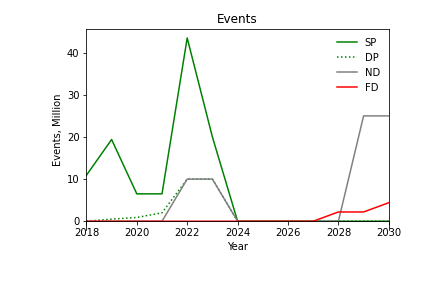
\includegraphics[width=0.8\textwidth]{IntroFigures/Events.png}
\end{dunefigure}

CPU and size/readout are drawn from the above estimates. We then make the following assumptions about data sizes and retention.  
Figures \ref{fig:est:disk,fig:est:tape,fig:est:cores} illustrate the estimated storage and CPU needs through 2030.  In the early years, \dword{pd} and \dword{nd} prototype tests dominate while commissioning and operation of the first (and second) \dword{fd} and the \dword{nd} become important after 2026. 

\begin{itemize}
\item Two copies of raw data are retained indefinitely
\item Commissioning data is marked test and one copy is retained on disk for 6 months. 
\item Reconstruction is performed on the full data sample once/year and 2 copies are retained on disk for 2 years.  
\item Analysis includes calibration and is  equivalent to reconstruction but produces smaller outputs. 
\end{itemize}

\begin{dunefigure}
[Disk estimates]
{fig:est:disk}
{Estimated size of various samples in PB. This estimate includes retention policies and multiple copies.}
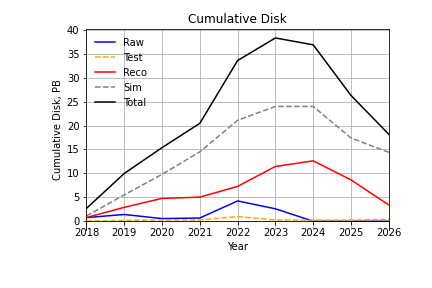
\includegraphics[width=0.8\textwidth]{IntroFigures/Cumulative-Disk.png}
\end{dunefigure}

\begin{dunefigure}
[Tape estimates]
{fig:est:tape}
{Estimated size of various samples in PB. This estimate includes retention policies and multiple copies.}
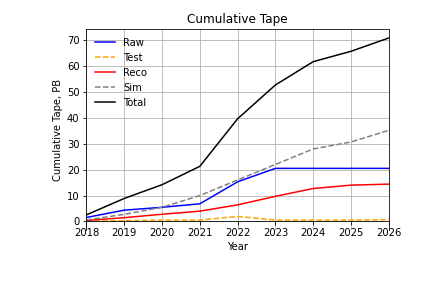
\includegraphics[width=0.8\textwidth]{IntroFigures/Cumulative-Tape.png}
\end{dunefigure}

\begin{dunefigure}
[Tape estimates]
{fig:est:cores}
{Estimated CPU needs for  various samples.  The units are present day cores assuming 70\% efficiency.}
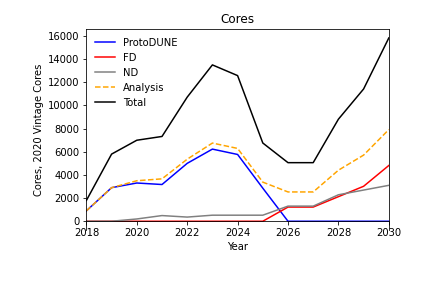
\includegraphics[width=0.8\textwidth]{IntroFigures/Cores.png}
\end{dunefigure}
\end{document}% (Heidi and Kirby)}  % Heidi and Kirby
\cleardoublepage

\documentclass[../main-00.tex]{subfiles}
\begin{document}
\chapter{Use Cases}
\label{ch:use}
\section{Introduction}

In this chapter we describe some of the known use-cases for DUNE computing.  We start with the protoDUNE cases, using lessons learned from the 2018 run to understand the performance of future far detector modules. 


%%%%%%%%%%%%%%%%%%%%%%%%%%%%%%%%


\section{ProtoDUNEdata: raw data acquisition, cataloging and storage}\label{sec:use:pdii-daq}



\subsection{ProtoDUNE Data: DAQ to Raw Data store}
The \dword{daq} and \dword{cisc} systems are expected to provide in close to real time:

\begin{itemize}
    \item Raw data from the \dword{tpc} and \dword{pd} detectors. 
    \item Information on run and trigger configuration
    \item Beam information
    \item Information on detector conditions. For example, granular information on the \dword{hv} is needed to study and compensate for \dword{hv} fluctuations. 
    \item Low level calibration constants such as gains that do not need extensive offline processing
    
\end{itemize}


The raw data are written to disk locally and then copied to the archive site (FNAL). Once the data are confirmed to be on tape, the local copy may be deleted.

A second copy of the raw data will be stored in a different archive. 

The run and trigger information, beamline  data, conditions and calibration constants are made available through separate data paths and stored in appropriate databases. In ProtoDUNE Run I, some of this information was transferred manually and stored in the \dword{sam} catalog.  DUNE document 22983 \cite{bib:docdb22983} describes the metadata strategy for ProtoDUNE II and DUNE. 


\section{ProtoDUNE data: reconstruction - hits}\label{sec:use:pdii}

Figure \ref{fig:ch:use:pdii} shows the data flow for regular reconstruction.  There are in principle, multiple stages in reconstruction that are well suited to different computer architectures.  We expect the full \dword{fd} data processing to follow a similar path. 

\subsection{Raw data to reconstructed hits}

This step takes the raw waveforms, applies  basic channel-to-channel calibrations, removes noise and stuck bits and performs 2D deconvolution.   This processing step operates on large 2-D data arrays and may be suitable for different architectures than conventional pattern recognition. It is anticipated that this step will not need to be done frequently. 

The input data at this point are quite uniform, effectively bit streams from \dword{tpc} and \dword{pd} channels.  There are correlations between channels in \dword{tpc} data which require concurrent processing of multiple channels.  Segmentation at the level of a readout plane within an \dword{apa}  or \dword{lem} is desirable.  An uncompressed \dword{apa} plane is of order 10 MB of 12-bit words. 

The outputs are gaussian fits to the pulses 



\subsection{Hits to Calibration}

In this step, the processed hits from calibration samples (subsets of the full data, sometimes with special conditions) are run through specialized pattern recognition and used to derive high quality calibration constants which are stored in the conditions database for future use.   This step will likely be done many times, especially at experiment start.

\subsection{Hits to reconstructed interactions }
In this step, the improved calibration constants and raw hits are input to the full  pattern recognition and reconstructed interactions are output. Data quality can be monitored as part of this processing and stored. 

Here a wide range of algorithms may be used.  

\subsection{Interactions to Analysis}
The interaction data, which is in the output format supplied by the full reconstruction is reduced and reconfigured into analysis formats for use by users. 

In the long run this processing will be done as coherent production steps but is currently being done by small groups.

A typical \dword{pdsp} data or simulation sample reads in  of around 1,000-10,000 4-8 GB reconstructed files and produces much smaller tuple outputs for analysis.  These jobs stream using \dword{xrootd} and are IO bound. Preliminary monitoring studies indicate that average input rates of 30 MB/sec per process can be achieved within a single site, with aggregate rates of several GB/sec across multiple processes. We are currently mining data access records to measure rates and reliability as a function of source and sink. 

\subsection{Analysis}
Analysis samples should be small and useful.  Analysis codes should not need to read from the central databases but may access small local replicas. 


\begin{dunefigure}
[Data flow diagram for standard ProtoDUNE reconstruction]
{fig:ch:use:pdii}
{Data flow diagram for standard ProtoDUNE data reconstruction.}
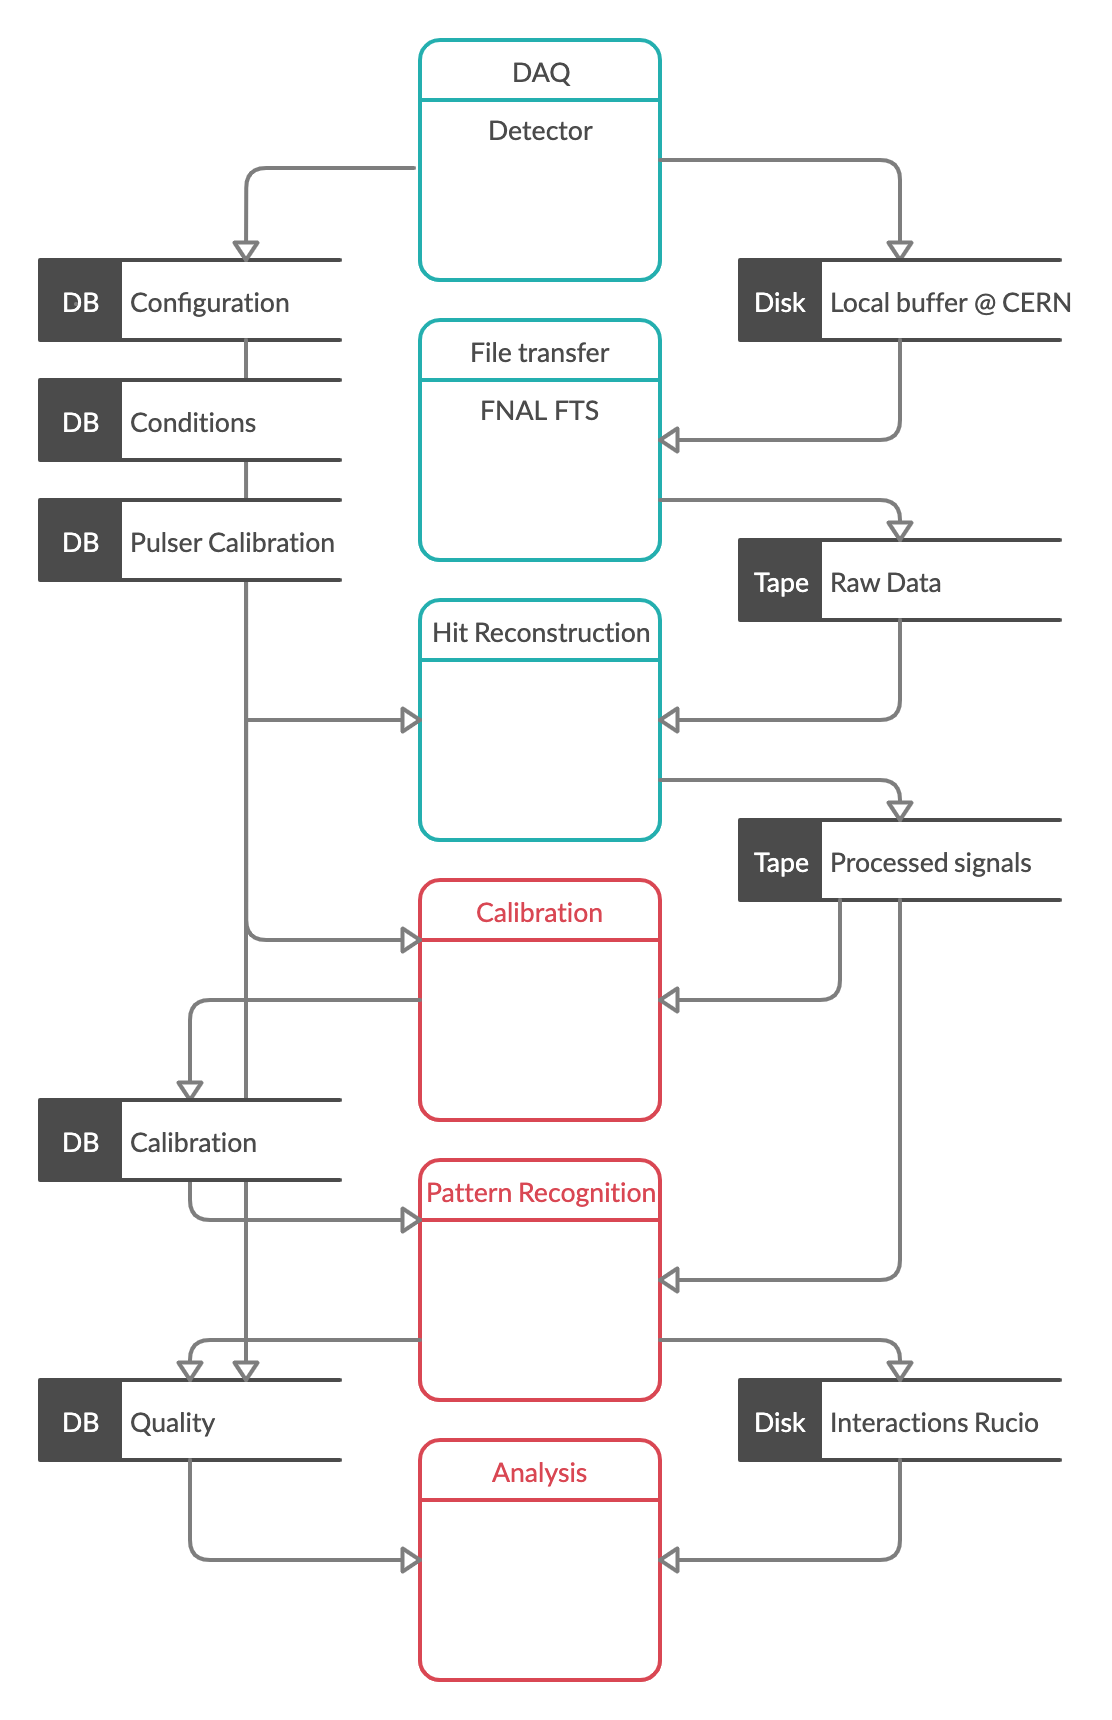
\includegraphics[width=0.8\textwidth]{graphics/IntroFigures/DataProcessingPDv1.png}
\end{dunefigure}
\pagebreak


%\section{Data reduction at FNAL before writing it out?}

%\section{Fast processing for data monitoring} 

\section{Normal  and SNB Far Detector: acquisition and reconstruction}
\label{sec:use:fdbeam}  %% fix label according to section

\begin{dunefigure}
[Data aggregation diagram for FD]
{fig:ch:use:fdagg}
{Data aggregation cases for the far detector. The top case shows information for normal beam or calibration readouts. A single file of $\sim 10$GB size contains several complete trigger readouts with their boundaries designated by the dashed lines.  TPC APA's, Photon Detector (PD),  trigger primitives and a trigger  are recorded for each trigger readout.  In addition, a manifest which describes the relations between the data is stored, either in the file or in metadata.  The bottom case is a supernova readout, in which thousands of 5-10 ms time slices must be read out over 100 sec.  The solid lines denote file boundaries. How data ordered, by geographical position or by team is not specified.}
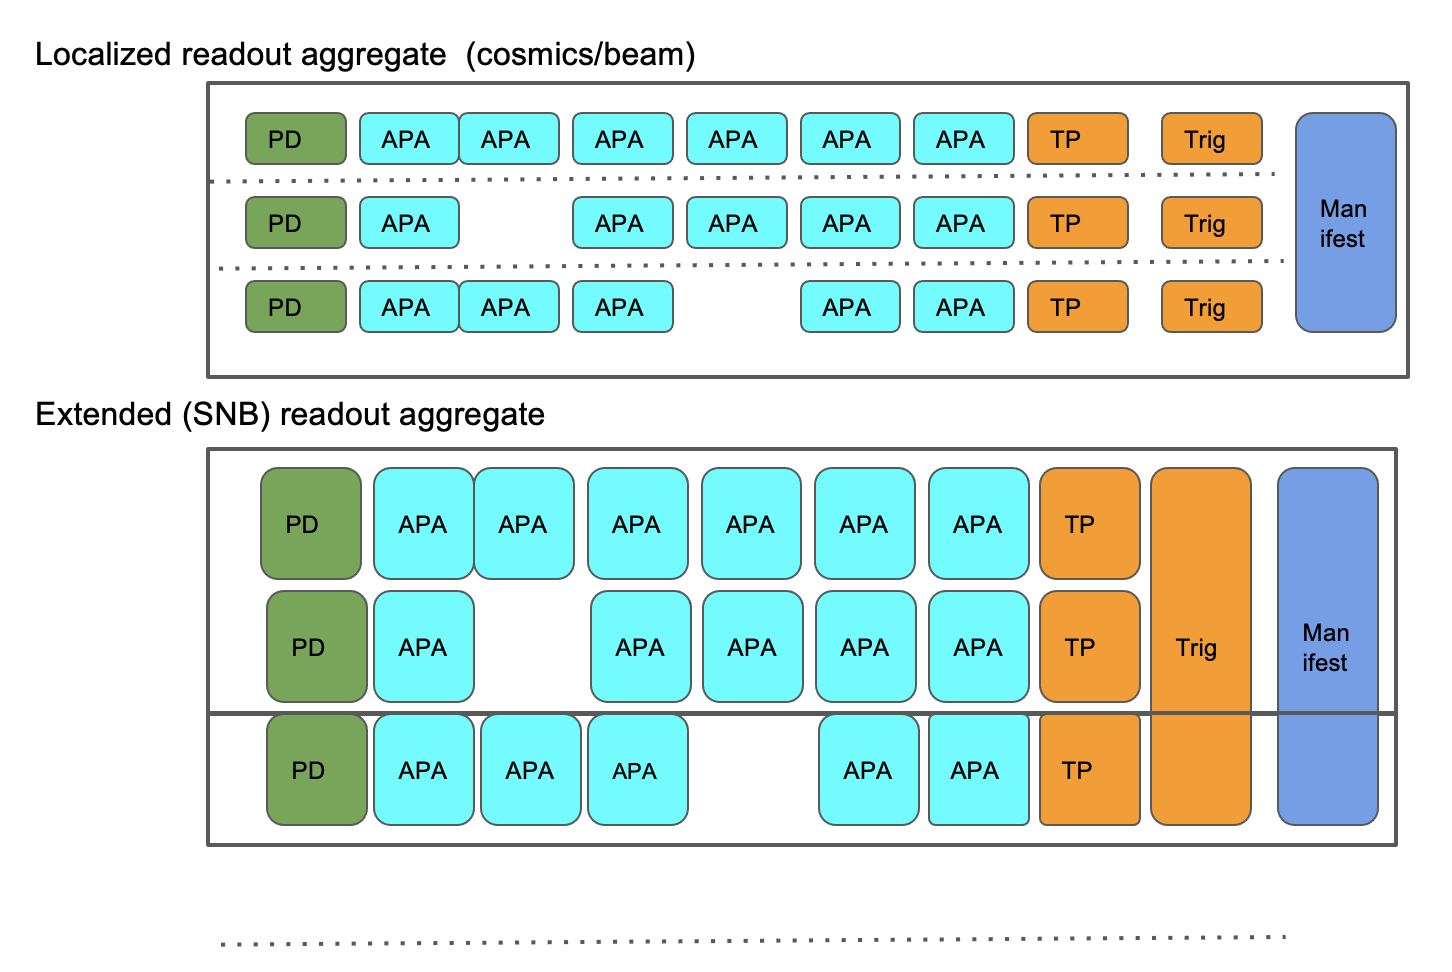
\includegraphics[width=0.8\textwidth]{graphics/IntroFigures/DataAggregation.png}
\end{dunefigure}
%\pagebreak

\subsection{ProtoDUNE simulation}

\fixme{need some text here on simulation}
 
\section{DUNE Beam Data: Beam data acquisition and reconstruction \hideme{ Mathew Muether/Tom Junk}}
\label{sec:use:ndbeam}  %% fix label according to section

\section{DUNE Simulation}  \fixme{Mathews' diagram} 

Simulation shares a reconstruction path with real data but begins differently.

\subsection{Beam simulation}\label{sec:use:beamsim}
Tbe neutrino beam is simulated using g4lbnf\cite{g4lbnf} a geant4 based simulation of the beamline components.  Intermediate interactions are stored so that cross section reweighting can be applied.  The beam simulation is generally done separately and beam files are stored and used when needed. 

%\subsection{Cosmic simulation?}

\todo{how big are events?  what are memory/CPU requirements}

The far and near detectors subtend very different solid angles so one has to simulate a very large number of events or use reweighting techniques to properly cover both. 

%\subsection{Cosmic simulation?}

\subsection{Interaction simulation}\label{sec:use:intmodel}
Next an event generator is used to simulate the primary interaction.  This step requires a reasonably accurate geometry for the detectors to account for different target materials and, for the near detector, different locations. Simulation parameters and reasonably detailed event information need to be stored to allow for subsequent reweighting.  

\subsection{Particle tracing}\label{sec:use:tracing}
The geant4 simulation package is then used to simulate the energy deposited by final state particles as they pass through the detector.  Both ionization and scintillation signatures need to be recorded.  

\subsection{Detector response simulation}\label{sec:use:detsim}
Once geant4 has simulated the energy deposit, detailed simulation of charge and light collection and electronics response can be done.  

\subsection{Overlay}\label{sec:use:overlay}
It is often useful to overlay real data on simulation to fully account for cosmic ray and upstream neutrino interactions. This adds complexity as the real data must be delivered to simulation jobs and be properly matched to the running conditions for the simulation.  The "electronics" signals from real data and simulation need to be mixed and stored.  The \dword{microboone} experiment has adapted \dword{larsoft} to do this and we plan to build on that experience. 

\todo{Discussion of overlay experience from MicroBooNE - Kirby}

\subsection{Reconstruction} \label{sec:use:mcreco}
Reconstruction and analysis can then be performed using the same methods as in section \ref{sec:use:pdii}.  Due to the large amount of interaction and intermediate step information kept for studies, simulated events are often several times the size of real data.  A significant question, given the size of events, is whether it may be more efficient to regenerate than to store all the information needed for reweighting. 


\todo{add a table showing \# of events, CPU and memory footprint for each step}









\section{Oscillation analysis} Chris Backhouse?  Chris Marshall? 
\label{sec:use:osc}

\section{Supernova data: acquisition and fast reconstruction}
\label{sec:use:supernova}  %% fix label according to section

\subsection{Fast ( 1 day turnaround)} \fixme{Priority for readout?}

\subsection{Full Supernova}

\section{Solar/BSM analysis}
\label{sec:use:BSManalysis}

\section{Calibration data: acquisition, reconstruction and use}
\label{sec:use:calib}  %% fix label according to section

\section{Hardware database use case} \fixme{Paul has an example}
\label{sec:use:hdb} 

\section{What's missing?}
\label{sec:use:todo}



\todo{Produce table that shows, input/output/CPU and memory footprint for each stage of processing - Heidi gathers info}



\end{document} % if using subfiles
\cleardoublepage

\part{Algorithms and Frameworks} %  Tom Junk, David Adams


\documentclass[../main-00.tex]{subfiles}
\begin{document}

\chapter{Frameworks \hideme{Andrew Norman, Paul Laycock, Mathew Muether}}
\label{ch:fworks}
\todo{Define all the fun data concepts  - Schellman}
%%%%%%%%%%%%%%%%%%%%%%%%%%%%%%%%
%\section{xyz}
%\label{sec:fworks:xyz}  %% fix label according to section

\section{Current status \hideme{ Junk/Muether}}

The data processing framework in use by the \dword{fd} simulation and reconstruction efforts, the \dword{protodune} detectors and \dword{ndgar} is \dword{art}.  The \dword{art} framework defines the data processing loop, manages memory, interfaces to I/O tools, defines uniform mechanisms for defining, associating, and persisting data products, provides a uniform mechanism for job configuration, stores job configuration information in its output files, and manages messages, random numbers and exceptions.  The \dword{art} framework runs user code that is provided as {\it plug-ins}, which are built as separate shared object libraries that can be dynamically selected and loaded at runtime.  The \dword{art} framework is also used by the NOvA, Muon g-2, MicroBooNE, ICARUS, LArIAT and ArgoNeuT collaborations.  The \dword{art} framework evolved from CMS's software framework and started being used by intensity-frontier experiments in 2011~\cite{Green:2012gv}. It is developed, maintained and supported by Fermilab's \dword{scd}.

The \dword{larsoft} toolkit is a collection of \dword{art} plug-ins and associated algorithm code, configuration files, and static data such as geometry specification files and photon visibility maps.  \dword{larsoft} provides the interface to event generators like \dword{genie} and \dword{corsika}, detector simulation via \dword{geant4}, custom simulation and reconstruction software, event displays and tutorials.  Experiment-specific metadata plug-ins assist in batch workflow organization.  \dword{larsoft} is supported by Fermilab's \dword{scd}, though much of the software has been contributed by participating experiment collaborations.

TODO - paragraph on SSRI/\dword{tms}

\dword{garsoft} is patterened on \dword{larsoft}.  It is a software toolkit for simulating and reconstructing data from \dword{ndgar}.  It is based on the \dword{art} framework.  Like \dword{larsoft}, it provides interfaces to event generators and \dword{geant4}, custom simulation and reconstruction software, and event displays.  It also provides simulation and reconstruction for \dword{ndgarlite}.  \dword{garsoft} is written, maintained, and supported by the DUNE collaboration.

The \dword{ndlar} software effort is currently being developed as a series of standalone tools for simulating and reconstructing pixel-based \dword{lartpc} data.  Toolchains have been developed for analyzing SingleCube prototype data.

The \dword{sand} software effort benefits from long experience with the \dword{kloe} detector, which provides the magnet and calorimeter.  New software is developed for the \dword{3dst} and other components of SAND.  Flexibility is important at this stage in order to allow studies of different detector designs to fill in between the \dword{3dst} and the calorimeter, such as a gaseous \dword{tpc}.  Because \dword{sand} will not move off axis with \dword{ndlar} and \dword{ndgar}

\section{Requirements summary}
% Taken from vCHEP paper
Modern HEP software frameworks are in the process of addressing the increasing heterogeneity of computing architectures that are redefining the computing landscape, work that is closely followed by the HEP Software Foundation~\cite{Alves:2017she, Calafiura:2018rwe}. The DUNE collaboration is keen to leverage this work to minimise the development effort needed for its own software framework.  Nevertheless,
given the unique challenges that DUNE data pose, the collaboration assembled a task force to define the requirements for its software framework.  Some of their findings are detailed in the following.

\subsection{Data and I/O layer}
Following the discussion on raw data processing, the DUNE software framework must have the ability to change its unit of data processing with extreme flexibility and ensure that memory is treated as a precious commodity.  
It must be possible to correlate these units to DUNE data-taking "events" for exposure accounting, and experiment conditions.
Partial reading of data is another strong requirement needed to keep memory usage under control.  There must be no assumptions on the data model, the framework must separate data and algorithms and further separate the persistent data representation from the in-memory representation seen by those algorithms.  DUNE data is well suited to massively parallel processing compute architectures, so the framework will need to have a flexible I/O layer supporting multiple persistent data formats as different formats may be preferred at different stages of data processing.  The sparsity of DUNE data also imply that compression will play an important role in controlling the storage footprint, especially for raw data, and the sparsity of physics signals further emphasise support for data reduction (skimming, slimming and thinning) in the framework.  The framework needs to be able to handle the reading and writing of parallel data streams, and navigate the association (if any) between these streams with a critical need to allow experiment code to mix simulation and (overlay) data.

\subsection{Concurrency}
Many aspects of DUNE data processing are well suited to concurrency solutions and the framework should be able to offload work to different compute architectures efficiently, facilitate access to co-processors for developers and schedule thread-safe and non-thread-safe work.  It must be possible to derive the input data requirements for any algorithm in order to define the sequence of all algorithms needed for a particular use case, and it must be possible to only configure those components required for that use case.

\subsection{Reproducibility and provenance}
As previously stated, the framework must ensure that memory is treated as a precious commodity, implying that intermediate data products cannot occupy memory beyond their useful lifetime.  Nevertheless, reproducibility is a key requirement of any scientific tool and the framework must provide a full provenance chain for any and all data products which must include enough information to reproduce identically every persistent data product. By definition, the chain will also need to include sufficient information to reproduce the transient data passed between algorithm modules, even though the product is not persisted in the final output.
It is also highly desirable that the framework broker access to random number generators and seeds in order to guarantee reproducibility.  All of the preceding considerations imply that the software framework will need a very robust configuration system capable of handling the requirements in a consistent, coherent, and systematically reproducible way.

\subsection{Analysis}
Machine learning is already heavily used in analysis of ProtoDUNE data and the framework should give special attention to machine learning inference in the design, both to allow simple exchanges of inference backends and to record the provenance of those backends and all necessary versioning information.  Finally, the framework should be able to work with both Near Detector and Far Detector data on an equal footing, and within the same job.


\section{HSF software frameworks review \hideme{Norman/Laycock}}

Ideally we can cite an HSF review here \cite{HSF-fwk-review}.  The review studied the physics requirements laid out by the task force and gave expert feedback on those requirements, further distilling them to technical requirements.  The review found that several frameworks are capable of fulfilling many of \dword{dune}'s requirements, key requirements are the following:

\begin{itemize}
    \item one
    \item two
    \item three
    \item four
    \item five
\end{itemize}

\subsection{The closest match to \dword{dune}'s requirements}

Following on from the HSF review, the \dword{dune} collaboration assessed the selection of frameworks suggested by HSF that warranted further investigation.  The framework that matches most closely to \dword{dune}'s needs is (drum roll).

\subsection{Missing functionality}

Even if the Captain Amazing framework is amazing, and it really is, there are still requirements that are not completely fulfilled by it.  These are:

\begin{itemize}
    \item one
    \item two
\end{itemize}

\section{Plan to go forward \hideme{ Norman}}

Development plan.

%This plan was further reviewed by the HSF, maybe.
%
%\subsection{HSF recommendation for a path forward}
\end{document}  % Paul and Andrew
\cleardoublepage

\chapter{Databases - (Paul Laycock and Norm Buchanan)}
\label{ch:db}

%%%%%%%%%%%%%%%%%%%%%%%%%%%%%%%%
\section{Introduction}
\label{sec:db:intro} 

In order to accommodate the large range of metadata that will be tracked by DUNE, the DUNE DB structure is made up of several databases. It is critical that users are able to access any metadata required throughout the full data processing and analysis chain with as little burden as possible. To achieve this users will interact with a centralized interface rather than with the individual databases. 

It is expected that there will be reconstruction and analysis jobs distributed across large numbers of traditional and high-performance computing systems and the database access will need to be able to scale appropriately.

\section{Conditions Database}
\label{sec:db:conditions} 

The configuration database is the central database that offline users, and processes, will interact with. This will reduce the number of database connections required by offline processes, ensuring that jobs will be "lightweight" and minimizing processing time.

The conditions database will contain interpolated (eg. slow controls) and non-interpolated (eg. run configurations) information. Interpolated information may more naturally be keyed by time-stamps while configurations are more naturally keyed by run number. Tools will need to be developed to handle these two cases of database content. 

\section{Run Configuration Database}
\label{sec:db:config}  

The run configuration database contains the intended configuration of the detectors during data collection - physics or otherwise. 

Metadata contained in the run configuration database includes, hardware settings, run type, and run start and end times. Table~\ref{table:runconfig} contains some examples of typical metadata that will be contained in the run configuration database. 

\begin{table}[h!]
\centering
 \begin{tabular}{||l| l ||} 
 \hline
 Metadata Value & Type  \\ [0.5ex] 
 \hline\hline
Start of run   &  Time \\ \hline
Readout window size  & Integer  \\ \hline
Readout trigger type  &  Integer \\ \hline
Readout firmware version &  Integer \\ \hline
Baseline start &  Integer \\ \hline
Shifter comments &  Text \\ \hline
Run end status & Integer \\ [1ex] 
\hline
\end{tabular}
\caption{Example metadata values and types stored in the run configuration database.}
\label{table:runconfig}
\end{table}

The majority of run configuration metadata comes form the configuration files used by the data acquisition system during run execution. Some additional metadata collected at the end of the run - or shortly thereafter may also be included. Examples are run completion status and comments made by the shifter during the run or in run-related checklists.

Parameters used to configure the run will be collected and packed into JSON-formatted blocks in a single "blob" corresponding to a DAQ run.   

\section{Data Quality and Monitoring Database}
\label{sec:db:dqm}  

The data quality and monitoring (DQM) database contains metadata derived from data collected during operation of the DUNE detectors. The DQM DB is an online database and interfaces with the conditions database directly or via an offline data quality database.

\section{Offline Calibration Database}
\label{sec:db:calib} 

The calibration database contains calibration constants determined from collected data corresponding to intervals of validity (IOV). The calibration metadata will result from offline calculations using data collected from the DUNE detectors.

There will generally be multiple versions of calibration constants corresponding to the same interval of validity. These versions will be contained within the database and accessible to users.  


\section{Slow Control Database}
\label{sec:db:slowcontrol}  

The slow control DB contains metadata specific to the state of detector during the time data were collected as well as before and after. Examples of slow control metadata are measurements of power supply voltages and currents and temperatures. Each slow control quantity corresponds to a particular device. The slow control DB metadata is time-indexed and different devices can be sampled at different rates.

\begin{table}[h!]
\centering
 \begin{tabular}{||l| l ||} 
 \hline
 Metadata Value & Type  \\ [0.5ex] 
 \hline\hline
PS1 Voltage  & float \\ \hline
PS1 Current  & float  \\ \hline
PS1 Temp  &  float \\ \hline
PS2 Voltage & float \\ [1ex] 
\hline
\end{tabular}
\caption{Example metadata values and types stored in the slow control database.}
\label{table:sc}
\end{table}

\section{Beam Conditions Database - IFBeam}
\label{sec:db:ifbeam}  

The beam conditions database, IFBeam~\cite{ifbeam} will contain metadata related to the condition extracted beam and corresponding diagnostics.  The functional form of this database is essentially the same as that of the slow control database. A large number of devices are sampled into the IFBeam DB. The IFBeam metadata transferred to the conditions DB will be a coarser subset of the original set.

Quantities contained in the IFBeam DB include beam currents, horn currents and polarities, and beam monitoring instrument metadata.

\begin{table}[h!]
\centering
 \begin{tabular}{||l| l ||} 
 \hline
 Metadata Value & Type  \\ [0.5ex] 
 \hline\hline
Horn 1 Polarity &  Integer \\ \hline
Horn 2 Polarity  & Integer  \\ \hline
Beam current & Float \\ [1ex] 
\hline
\end{tabular}
\caption{Example metadata values and types stored in the run configuration database.}
\label{table:ifbeam}
\end{table}

\section{Hardware Database}
\label{sec:db:hwdb}  

The purpose of the hardware database is to track the lineage of hardware components. In this context a component can be a sub-detector module or any of the individual parts comprising it. For example, a readout board is a component as is the a mezzanine daughter board or programmable logic chip mounted on the readout board. The lowest level component tracked within the HWDB will be unique to the corresponding hardware system.

Hardware DB metadata will pertain to the following stages of component lifetime:

\begin{itemize}
\item Procurement 
\item Fabrication
\item Quality control testing
\item Shipping and Storage
\item Installation
\item Maintenance 
\end{itemize}

The relationships between components will be reflected in the HWDB. Metadata corresponding to multiple instances of events such as QC tests will be handled using time series within the database. 

\section{Service and Maintenance}
\label{sec:db:service}  

Most, if not all, of the DUNE databases will operate in advance of the full DUNE experiment coming online and these databases will need to be maintained and serviced once they are operational. 

The second run of the ProtoDUNE experiment (ProtoDUNE II) will employ a suite of databases that will be the precursors to the full database system that will be in place for DUNE. Each of these databases (run configuration, beam instrumentation, conditions, slow controls, and hardware) will require stable monitoring, maintenance, and service to address operational issues that will arise in the lead up to and during the running of the ProtoDUNE II experiment. 

Monitoring will be achieved using automated web-based tools [ref needed] and responses to offline database issues will be made within an 8-hour period corresponding to a typical operation or production "shift". For ProtoDUNE II databases will be located at both Fermilab and CERN, both of which have a long history of database support.


\todo{Need a section on R+D needs}

\todo{add person power estimates, possibly } % Norm and Paul 
\cleardoublepage

\chapter{Applications overview}
\label{ch:appl}

%%%%%%%%%%%%%%%%%%%%%%%%%%%%%%%%
\section{xyz}
\label{sec:appl:xyz}  %% fix label according to section

 % Tom and Mathew and Elisabetta
\cleardoublepage

\section{Reconstruction Algorithms\hideme{ TRJ}}
\label{sec:algo:reco}

This section gives brief outlines of reconstruction algorithms in use in DUNE's detectors.  The \dword{fd} will consist of four modules, at least three of which will be \dwords{lartpc}, and the fourth module, the module of opportunity, has yet to be designed.  The near detector will have a \dword{lartpc}, in addition to a muon spectrometer and/or \dword{ndgar}, and \dword{sand}, each of which consists of multiple subdetectors.  \dword{ndlar} will have a pixel-based readout, which enables a much easier reconstruction of densely-packed objects.  The \dword{pdsp} detector is also a \dword{lartpc}, and a vertical-drift prototype is planned.

\subsection{Liquid Argon TPC Reconstruction}
\label{sec:algo:reco:lartpc}

\subsubsection{Wire and Strip-Based Liquid Argon TPC Recontruction}
\label{sec:algo:reco:lartpc:wirestrip}

Reconstructing events in a \dword{lartpc} is challenging.  Each trigger record contains a large number of waveforms, one for each readout channel.  In \dword{pdsp}, the waveforms typically were 6000 time ticks long, with one \dword{adc} sample per time tick.  A detailed description of the reconstruction procedures, starting with these waveforms, is given in~\cite{Abi:2020mwi}, and summarized briefly here.

Typically, data from a single-phase \dword{lartpc} \dword{daq} are stored as compressed sequences of data frames, containing 128 or 256 channels' worth of data on each time sample.  These must be decompressed and rearranged into sequences of \dword{adc} values corresponding to the original waveforms.  Additional decoder modules are run to unpack \dword{pds}, \dword{crt} trigger and timing \dword{daq} fragments.
From there, mitigations are applied to correct, as best as possible, known failures of the front-end electronics.  As yet, these are only needed for the TPC readout electronics.  A particular failure mode in \dword{pdsp} is the sticky-code problem, which is mitigated by interpolating neighboring ADC samples in time.  Channel-to-channel gain corrections are applied, correlated noise is filtered out, the pedestal is found, and a correction is made for the \dword{ac} coupling between the preamp and the ADC.  The ADC mitigation, correlated noise removal, gain correction, pedestal finding and \dword{ac} coupling corrections are grouped into the data preparation module.  The \dword{wirecell} toolkit provides a two-dimensional deconvolution in wire index and charge arrival time, and it associates charge in the three views to produce a three-dimensional image of the charge locations where it was produced.  

The calibrated, filtered, deconvolved waveforms are then used as input to a hit-finding algorithm, which identifies peaks in the waveforms and fits Gaussians to each proposed peak.  These hits are then used as inputs to general reconstruction algorithms, such as the SpacePointSolver Pandora, TrajCluster, and PMA, which identify clusters, tracks and showers in three dimensions by associating objects in the three two-dimensional views.  The calorimetry modules sum up and calibrate the charge deposits for use in energy reconstruction and \dword{pid}.  The parameters of the clusters, tracks and showers are stored in ROOT trees that end users can analyze rapidly and repeatedly.

Additional modules find hits in the photon detector waveforms and group them into clusters called flashes.  The \dword{crt} data are analyzed in dedicated modules that produce associations between hits in the upstream and downstream \dword{crt} modules for use in analyses.

Separating track-like energy deposits from shower-like deposits is a key part of many DUNE analyses.  This is accomplished with a \dword{cvn} called {\tt EmTrackMichelID} in Table~\ref{tab:protodune_cpu_reco_by_module}.  It is one of the most CPU-intensive operations in the \dword{pdsp} reconstruction chain, when the algorithm is run on a grid node lacking a GPU.  Recently, however, a \dword{gpuaas} technique has been developed~\cite{Wang:2020fjr}, enabling a speedup of the order of a factor of ten, though it depends on the ratio of CPU-only nodes to GPU resources.


\subsubsection{Pixel-Based Liquid Argon TPC Recontruction}
\label{sec:algo:reco:lartpc:pixels}

\begin{dunetable}
[Processing time for reconstruction modules for a \dword{pdsp} event]
{l r}
{tab:protodune_cpu_reco_by_module}
{Wall-clock module execution times for the reconstruction of a typical ProtoDUNE-SP event, in seconds.  The event is a data event from Run 5809, a 1 GeV beam run.}
Module Label & time/event (sec)\\ \toprowrule
RootInput(read)                          &     0.147283          \\
timingrawdecoder:TimingRawDecoder        &     0.0095498         \\
ssprawdecoder:SSPRawDecoder              &     0.126099          \\
crtrawdecoder:CRTRawDecoder              &     0.0181903         \\
ctbrawdecoder:PDSPCTBRawDecoder          &     0.0204753         \\
beamevent:BeamEvent                      &      1.6154           \\
caldata:DataPrepByApaModule              &      83.0324          \\
wclsdatasp:WireCellToolkit               &      79.8616          \\
gaushit:GausHitFinder                    &      1.56342          \\
nhitsfilter:NumberOfHitsFilter           &    0.00177549         \\
reco3d:SpacePointSolver                  &      9.44157          \\
hitpdune:DisambigFromSpacePoints         &      1.52541          \\
pandora:StandardPandora                  &      39.8787          \\
pandoraWriter:StandardPandora            &     0.370009          \\
pandoraTrack:LArPandoraTrackCreation     &      4.57221          \\
pandoraShower:LArPandoraShowerCreation   &      3.73432          \\
pandoracalo:Calorimetry                  &      2.11152          \\
pandoracalonosce:Calorimetry             &      1.90852          \\
pandorapid:Chi2ParticleID                &     0.0115046         \\
pandoracali:CalibrationdEdXPDSP          &     0.106919          \\
pandoracalipid:Chi2ParticleID            &    0.00851985         \\
pandoraShowercalo:ShowerCalorimetry      &      3.26953          \\
pandoraShowercalonosce:ShowerCalorimetry &      3.17698          \\
emtrkmichelid:EmTrackMichelId            &      233.794          \\
ophitInternal:OpHitFinder                &     0.0190084         \\
ophitExternal:OpHitFinder                &    0.00828164         \\
opflashInternal:OpFlashFinder            &     0.0172739         \\
opflashExternal:OpFlashFinder            &    0.000597182        \\
opslicerInternal:OpSlicer                &     0.0184422         \\
opslicerExternal:OpSlicer                &    0.00538796         \\
crttag:SingleCRTMatchingProducer         &     0.0231673         \\
crtreco:TwoCRTMatchingProducer           &     0.0128138         \\
anodepiercerst0:T0RecoAnodePiercers      &      1.07673          \\
pandora2Track:LArPandoraTrackCreation    &      11.6525          \\
pandora2calo:Calorimetry                 &      4.95932          \\
pandora2calonosce:Calorimetry            &      4.55118          \\
pandora2pid:Chi2ParticleID               &     0.0211641         \\
pandora2cali:CalibrationdEdXPDSP         &     0.0867829         \\
pandora2calipid:Chi2ParticleID           &     0.0206842         \\
pandora2Shower:LArPandoraShowerCreation  &      4.17815          \\
pandora2Showercalo:ShowerCalorimetry     &      4.1729           \\
pandora2Showercalonosce:ShowerCalorimetry&      3.83562          \\
TriggerResults:TriggerResultInserter     &     0.000349372        \\
RootOutput                               &    2.8912e-05         \\
RootOutput(write)                        &     2.79458               \\
{\bf Total:}                             &     {\bf 507.881}      \\
    \toprowrule
\end{dunetable}

\subsubsection{Pixel-Based Gaseous Argon TPC Recontruction}
\label{sec:algo:reco:gartpc:pixels}

The \dword{ndgar} consists of two primary detectors -- a copy of the ALICE pixel-based \dword{tpc} in a 10-bar gas consisting predominantly of argon, surrounded by a calorimeter and a superconducting magneti coil.  A muon system is envisaged outside of the calorimeter but is not included in the simulation or the reconstruction at the time of writing.  Data are unpacked and hits are found on the per-readout-pad waveforms, similarly to how the initial stages of reconstruction for a \dword{lartpc} are followed.  Hits are then clustered into TPC clusters, which reduces the memory and CPU usage of subseuqent steps, and also increases the spatial resolution of individual clusters.  Vector hits are found by grouping TPC clusters into short line segments, and the vector hits themselves are grouped into track candidates by a pattern recognition module.  A track fit based on a Kalman filter then finds the best estimates of the track parameters.  Vertices are then found using tracks with nearby endpoints.  Because there is a cathode in the middle of the drift volume in the nominal design, a cathode stitch module is then run to associate track segments on either side of the cathode, bring them together by solving for the best interaction time that lines the segments up, and also moves the associated tracks and vertices.  Vees ($K^0_s$ and
$\Lambda^0$ candidates) are found by pairing nearby tracks together, optionally requiring a displacement from another vertex, and forming the invariant mass.  The calorimeter consists of a mixture of strips and pads.  Calorimeter hits are found in the \dword{sipm} waveforms provided by the calomrimeter \dword{daq}, and they are clustered together to form reconstructed three-dimensional energy deposit objects with positions, directions, and energies.

\begin{dunetable}
[Average processing time for reconstruction modules for GArSoft events consisting of just one interaction in the gas.  An actual spill will contain of order 60 interactions, mostly  in the calorimeter, though many tracks will pass through the gas.]
{l r}
{tab:garsoft_cpu_reco_by_module}
{Wall-clock module execution times for the reconstruction of a typical \dword{ndgar} event, in seconds.}
Module Label & time/event (sec)\\ \toprowrule
RootInput(read)                             &    0.000353765       \\
init:EventInit                         &    1.31275e-05       \\
hit:CompressedHitFinder                &    0.00488308        \\
tpcclusterpass1:TPCHitCluster          &     0.0091922        \\
vechit:tpcvechitfinder2                &     0.0103787        \\
patrec:tpcpatrec2                      &     0.0130245        \\
trackpass1:tpctrackfit2                &     0.014211         \\
vertexpass1:vertexfinder1              &    0.000851081       \\
tpccluster:tpccathodestitch            &     0.0269436        \\
track:tpctrackfit2                     &     0.0135842        \\
vertex:vertexfinder1                   &    6.19847e-05       \\
veefinder1:veefinder1                  &    9.96417e-05       \\
sipmhit:SiPMHitFinder                  &    0.00153375        \\
sscalohit:CaloStripSplitter            &     0.0547754        \\
calocluster:CaloClustering             &    0.00492599        \\
trkecalassn:TPCECALAssociation         &    0.000237503       \\
TriggerResults:TriggerResultInserter        &    2.36397e-05       \\
RootOutput                                  &    3.6783e-06        \\
RootOutput(write)                           &    0.214077         \\
{\bf Total}                                  &     {\bf 0.369802}         \\
   \toprowrule
\end{dunetable}
\section{Simulation Algorithms \hideme{TRJ}}
\label{sec:algo:sim}

\subsection{Beam simulation}
\label{sec:beamsim}

TBS

\subsubsection{Event Generators}
\label{sec:eventgen}

Extracting physics results from the DUNE experiment requires comparing the observed data with simulations which include detailed simulations of the physics processes under study as well as the response of the detectors.  The physics simulation is performed by the neutrino generators GENIE~\cite{Andreopoulos:2009rq}, NuWRO~\cite{NuWro2012}, GIBUU~\cite{Gallmeister:2016dnq}, NEUT~\cite{Hayato:2009zz}, and others.  Cosmic-ray simulations are performed with \dword{corsika}~\cite{Wentz:2003bp,Dembinski:2020wrp} for detectors on the surface, and MUSUN/MUSIC for detectors deep underground~\cite{Kudryavtsev:2008qh,LBNEDOCDB9673}.  Radiological decays are modeled with BXDECAY0~\cite{Ponkratenko:2000um} and the DUNE-specific RadioGen.

\subsubsection{Detector Simulation}
\label{sec:detsim}

The factorization of the simulation into a generation stage and a detector simulation stage is a common situation in collider experiments, such as ATLAS and CMS.  The fact that the interactions simulated by generators for collider physics happen inside an evacuated beampipe means that the details of the detector geometry and materials are not relevant for most event generation.  Lists of four-vectors of particles emerging from a primary vertex will suffice.  In a neutrino experiment, however, the detector material is the target material, and hence the generators must be aware of the detector geometry and materials, which affects the structure and performance of the generator code.  Currently, \dword{genie}, \dword{corsika}, MUSUN/MUSIC, BXDECAY0 and RadioGen are integrated with \dword{larsoft}.  \dword{genie} is integrated with \dword{garsoft}.


Two classes of simulation of DUNE's detectors exist at the time of writing.  Parameterized, or ``fast'' detector simulations involve smearing truth-level physics quantities based on expected detector performance metrics, such as acceptance and energy resolution.  These fast simulations are useful when optimizing detector designs, and for engaging physicists outside of the DUNE collaboration.  Full simulations, on the other hand, are based on detailed geometry models and \dword{geant4}~\cite{Agostinelli:2002hh,Allison:2016lfl}, and are needed for extraction of publication-level results.

In a \dword{geant4}-based simulation of a DUNE detector, \dword{geant4} is used only to simulate the interacting particles from neutrino scatters and other processes of interest, and energy depositions in the active detector material are stored as a distinct data product. The the many low-energy drifting electrons and scintillation photons are simulated in separate steps.  Drifting electrons are simulated parametrically using a model based on the measured drift velocity, longitudinal and transverse diffusion coefficients, and a parameterized model of space charge.  This last effect is particularly pronounced at \dword{pdsp}, giving rise to distortions in the apparent positions of particles of up to 30~cm.  Field distortions due to external imperfections such as the grounded electron diverters in \dword{pdsp}.

Once the electrons drift to the anode plane in wire-based \dwords{lartpc} in the simulation, a detailed two-dimensional model of the wire responses is applied~\cite{Abi:2020mwi}.  The two dimensions are wire number and time, and the effects of induced currents on neighboring wires are included in the simulation.  The electronics response function is folded in to a final model of the observed waveforms.  Simulated waveforms have been compared with real ones and are found to be very similar in \dword{pdsp}.
In the pixel-based \dword{ndlar} and \dword{ndgar}, the electronics simulation is at a simpler level, as the electronics have not been fully designed.

A large amount of code re-use and sharing via the design of \dword{larsoft} allows for the development of simulation algorithms for \dword{pddp}, the dual-phase far detector, and the Vertical Drift detector proposals.  Only the geometry, the field description, and the anode-plane models need to be updated; the rest of the simulation chain is re-used.

Photon propagation, scattering, absorption and detection are modeled in \dword{larsoft}'s simulation via a photon visibility lookup table, which gives the probability that a photon, emitted in a random direction at a specific location in the active volume of the detector, is detected by a specific photon detector.  The spatial granularity of the lookup table is a few cm.  This lookup table is populated with values that are computed from a \dword{geant4} simulation of scintillation photons in \dword{lar}, with the assumed values of the light attenuation length, the Rayleigh scattering length, the reflectivities of the surfaces inside the detector, and the transparency of the wire planes.  Scintillation photons are not yet simulated in the \dword{ndgar}, but photon detection systems are under consideration. 

\dword{ndgar} also has a calorimeter and a muon system.  The calorimeter is simulated via parameterized responses to the \dword{geant4}-simulated energy deposits, as are the responses to tracks in \dword{ndgarlite} and \dword{sand}.
\documentclass[../main-v1.tex]{subfiles}
\begin{document}
\section{Analysis Algorithms \hideme{Who - needed}}
\label{sec:algo:an}

DUNE's primary analysis framework is currently   the \dword{cafana} framework originally developed for the NOvA experiment \cite{Backhouse:2015wlj,  bib:cafana}. The HighLAnd framework used by T2K is also used for some analyses. 

\end{document}
\cleardoublepage

\part{Global Computing Model  } % McNab

\documentclass[../main-v1.tex]{subfiles}
\begin{document}
\chapter{Overview of Computing Model \hideme{McNab - draft}}
\label{ch:cm}

%%%%%%%%%%%%%%%%%%%%%%%%%%%%%%%%
\section{Introduction \hideme{Schellman/Herner - draft, update tables}}\label{ch:cm:intro} %\hideme{Schellman/McNab -needed}}
% Need a proper name

%SURF -> FNAL -> off site storage -> processing -> analysis

%Simulation -> storage -> analysis




The current DUNE global computing model is an organic extension of the \dword{fnal} \dword{fife} computing model, used for smaller Intensity Frontier experiments, to the full global DUNE collaboration.  This effort  has relied heavily on global infrastructure such as \dword{osg} and the \dword{wlcg} and was successful for the first small-scale \dword{protodune} tests. However, it needs substantial enhancement to cope with the anticipated data and processing volumes.  This chapter describes the current situation and proposals for future improvements. 

\subsection{Global Resources}

\dshort{dune} is a global collaboration %anne with contributions from institutions worldwide.  The 
for which the large-scale computing effort relies on %multi-national 
international contributions. The long-term strategy for computing resources is for primary raw data storage to reside at the large host labs (the \dword{cern} and \dword{fnal}) with computing resources such as %disk and CPU 
CPU and storage largely contributed by collaborating %countries. 
institutions. CPU contributions are provided by a large number of sites worldwide as shown in Figure~\ref{fig:prodsites}, while storage is concentrated at a few larger %international 
sites. Table~\ref{tab:coop:disk} shows the distribution of disk space pledges for 2021 and 2022, while Tables~\ref{tab:coop:sites} and~\ref{tab:coop:ussites} list the sites contributing CPU resources. 

\begin{dunefigure}

[Wall time distribution of Production jobs FY22]
{fig:prodsites}
{Distribution of wall time}
\includegraphics[width=0.5\textwidth]{graphics/Workflow/}
\end{dunefigure}

%This model builds on the highly successful tools developed by the WLCG and OSG for LHC computing.  As DUNE's needs are substantially smaller that those of the large LHC experiments we can be confident that the existing infrastructure can be incrementally augmented to meet DUNE's requirements. 

%\section{Current Global Computing Model}
%\todo{HMS done  Must update pledges}

\begin{dunetable}
[National disk pledges]{llrr}{tab:coop:disk}
{Disk pledges in PB for 2021 and 2022.}
Country/Lab	&	Name	&	2021	&	2022	\\
\dword{fnal}	&	\dword{fnal}	&	2.2	&	7.6	\\
\dword{cern}	&	\dword{cern}	&	2.2	&	3.0	\\
\dword{bnl}	&	\dword{bnl}	&	0.5	&	0.5	\\
United Kingdom	&	GridPP	&	4.0	&	4.0	\\
France	&	CC-IN2P3	&	0.5	&	0.5	\\
Spain	&	PIC Tier-1	&	0.5	&	0.72	\\
Netherlands	&	NL/LHC Tier-1	&	1.9	&	1.8	\\
Czechia	&	CZ-Prague-T2	&	0.3	&	1.0	\\
%BR	&	CBPF	&	0	&		\\
India	&	TIFR	&	0.75&	0.75\\
Russian Federation	&	JINR	&	-	&	0.5	\\
\hline
Total pledge	&		&	12.85	&	18.97	\\
Total request & & 20.4 & 27.3 \\
\end{dunetable}



%\tiny
\begin{dunetable}
[List of DUNE Compute Sites]
{l l r l}{tab:coop:sites}
{List of non-US international DUNE compute sites as of December 2021.  Sites with substantial \dword{rucio} controlled disk are noted.}
Site name	&	RC Site	&	Disk	&	Country	\\
\hline
BR\_CBPF	&	BR\_CBPF	&		&	Brazil\\
BR\_UNICAMP	&BR\_UNICAMP	&		&	Brazil\\
CA\_Victoria	&	CA\_Victoria	&		&	Canada\\
CERN	&	CERN-PROD	&	Yes	&	Switzerland\\
CH\_UNIBE-LHEP	&	UNIBE-LHEP	&		&	Switzerland\\
CZ\_FZU	&	FZU	&	Yes	&	Czechia\\
ES\_CIEMAT	&	CIEMAT-LCG2	&		&	Spain\\
ES\_PIC	&	pic	&	Yes	&	Spain\\
FR\_CCIN2P3	&	IN2P3-CC	&	Yes	&	France\\
IN\_TIFR	&	IN\_TIFR	&	Yes	&	India\\
NL\_NIKHEF	&	NIKHEF-ELPROD	&		&	Netherlands\\
NL\_SURFsara	&	SURFsara	&	Yes	&	Netherlands\\
RU\_JINR	&	JINR\_CONDOR\_CE	&	Yes	&	Russian Federation\\
UK\_Bristol	&	UKI-SOUTHGRID-BRIS-HEP	&		&	United Kingdom\\
UK\_Brunel	&	UKI-LT2-Brunel	&		&	United Kingdom\\
UK\_Edinburgh	&	UKI-SCOTGRID-ECDF	&		&	United Kingdom\\
UK\_Imperial	&	UKI-LT2-IC-HEP	&		&	United Kingdom\\
UK\_Lancaster	&	UKI-NORTHGRID-LANCS-HEP	&	Yes	&	United Kingdom\\
UK\_Liverpool	&	UKI-NORTHGRID-LIV-HEP	&		&	United Kingdom\\
UK\_Manchester	&	UKI-NORTHGRID-MAN-HEP	&	Yes	&	United Kingdom\\
UK\_Oxford	&	UKI-SOUTHGRID-OX-HEP	&		&	United Kingdom\\
UK\_QMUL	&	UKI-LT2-QMUL	&	Yes	&	United Kingdom\\
UK\_RAL-PPD	&	UKI-SOUTHGRID-RALPP	&		&	United Kingdom\\
UK\_RAL-Tier1	&	RAL-LCG2	&	Yes	&	United Kingdom\\
UK\_Sheffield	&	UKI-NORTHGRID-SHEF-HEP	&		&	United Kingdom\\

\end{dunetable}


\begin{dunetable}
[List of US DUNE Compute Sites]
{l l r }{tab:coop:ussites}
{List of US DUNE compute sites as of December 2021.  Sites with substantial rucio controlled disk are noted.}
US\_UConn-HPC	&	UConn-HPC	&	Disk\\
US\_BNL	&	BNL-SDCC-CE01	&	Yes	\\
US\_Caltech	&	CIT\_CMS\_T2	&	\\
US\_Clemson	&	Clemson-Palmetto	&	\\
US\_Colorado	&	UColorado\_HEP	&	\\
US\_Florida	&	UFlorida-HPC	&	\\
US\_FNAL	&	GPGrid	&	Yes	\\
US\_KSU	&	BEOCAT-SLATE	&	\\
US\_Lincoln	&	Rhino	&	\\
US\_Michigan	&	AGLT2	&	\\
US\_MIT	&	MIT\_CMS	&		\\
US\_MWT2	&	MWT2	&		\\
US\_Nebraska	&	Nebraska	&	\\
US\_NERSC & NERSC &   \\
US\_NMSU-DISCOVERY	&	SLATE\_US\_NMSU\_DISCOVERY	&	\\
US\_NotreDame	&	NWICG\_NDCMS	&	\\
US\_Omaha	&	Crane	&	\\
US\_PuertoRico	&	uprm-cms	&	\\
US\_SU-ITS	&	SU-ITS-CE2	&	\\
US\_UChicago	&	MWT2	&	\\
US\_UCSD	&	UCSDT2	&	\\
US\_Wisconsin	&	GLOW	&	\\
US\_WSU	&	WSU - GRID\_ce2	&	\\
\end{dunetable}


%anne 3/15 \section{Site characteristics}

\fixme{add a section which describes the various site types - HPS, normal, analysis, commercial services - I think this is already done in section 6.4 - Kirby (anne removed section header)}
%\todo{Add diagrams}

\section{Current Performance\label{ch:model:perf} \hideme{Schellman/Herner - draft}}. 

\dshort{dune} has performed multiple simulation and reconstruction passes on the \dword{pdsp} data and is running significant simulation campaigns for the \dword{fd} and \dword{nd} design and physics studies. The \dword{poms} and \dword{sam} described in Chapters~\ref{ch:datamgmt} and~\ref{ch:wkflow}, are highly instrumented and allow assessments of the performance of the global computing system in near-real time.  There are four major data/CPU access patterns:
\begin{itemize}
    \item Simulation requires little input (mainly beam flux files and photon libraries),  has a large memory footprint, uses significant CPU resources and writes back a few large files.
    \item Data reconstruction reads in large files, has an intermediate memory footprint and uses $\sim$10\,sec/MB of input data.  
    \item Data reduction reads the reconstructed data and produces small tuple outputs for further analysis.  Reduction uses $\sim0.1$\,sec/MB of input data and is generally IO limited.
    \item Data analysis consists of repeated access to smaller tuple outputs for calibration and parameter estimation.
\end{itemize}

Each of these use cases is best suited for a different combination of data/CPU resources and the global compute model should be able to allocate resources appropriately.  Currently the default configuration for all \dword{htc} jobs is for data delivery to be through \dword{xrootd} streaming. To understand the impact of this choice on effciency, we have used the \dword{sam} instrumentation to measure the \dword{xrootd} streaming performance for disk/CPU location combinations. 

\begin{dunefigure}
[Streaming speeds for reconstruction]
{fig:recospeed} 
{Streaming speeds for reconstruction jobs running at different locations. Raw data are stored at \dword{cern} and \dword{fnal}.  The histograms show the log10 of the inferred streaming rate (wall time/file size) for reconstruction jobs running at selected sites with different data sources.}
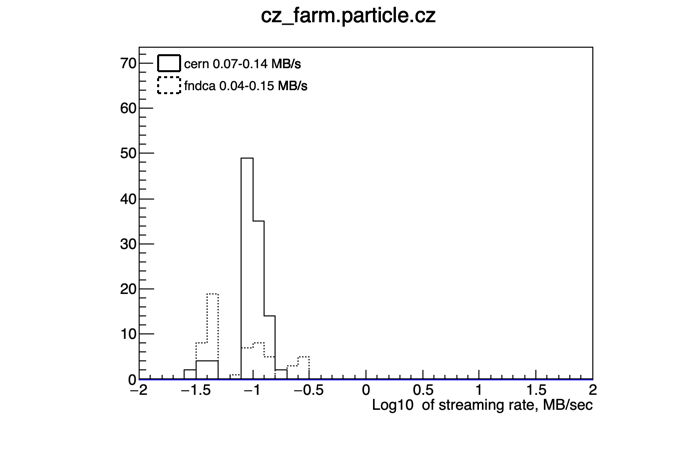
\includegraphics[width=0.45 \textwidth]{graphics/Workflow/dune_slow_2021_01_01_2021_04_30_0_cz_farm.particle.cz.png}
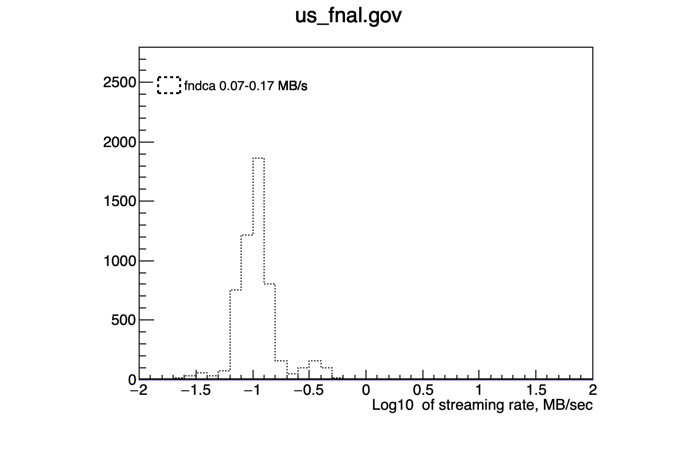
\includegraphics[width=0.45 \textwidth]{graphics/Workflow/dune_slow_2021_01_01_2021_04_30_0_us_fnal.gov.png}
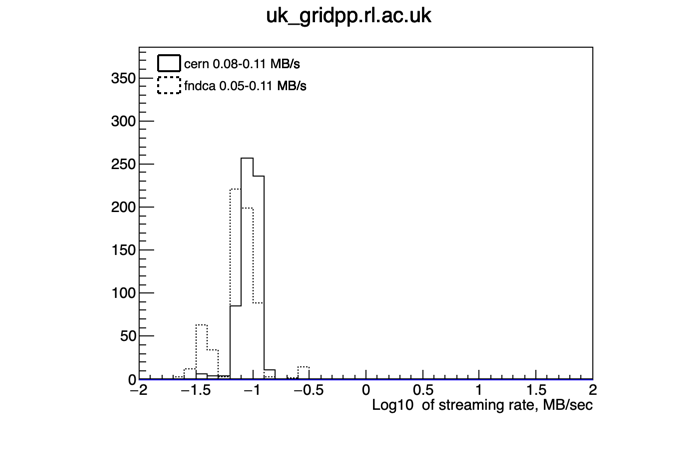
\includegraphics[width=0.45 \textwidth]{graphics/Workflow/dune_slow_2021_01_01_2021_04_30_0_uk_gridpp.rl.ac.uk.png}
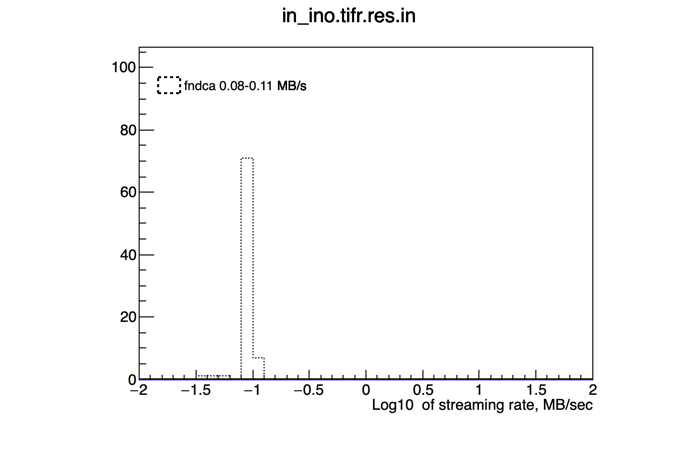
\includegraphics[width=0.45 \textwidth]{graphics/Workflow/dune_slow_2021_01_01_2021_04_30_0_in_ino.tifr.res.in.png}
\end{dunefigure}
%\todo{Get better figure}


\begin{dunefigure}
[Streaming speeds for tuple creation]
{fig:tuplespeed} 
{Streaming speeds for tuple creation jobs running at selected locations during a test in early January 2022. Reconstructed simulation files were located at sites in the UK and at Fermilab.  The histograms show the log10 of the inferred streaming rate (wall time/file size) for tuple creation jobs running at selected sites with different data sources.}
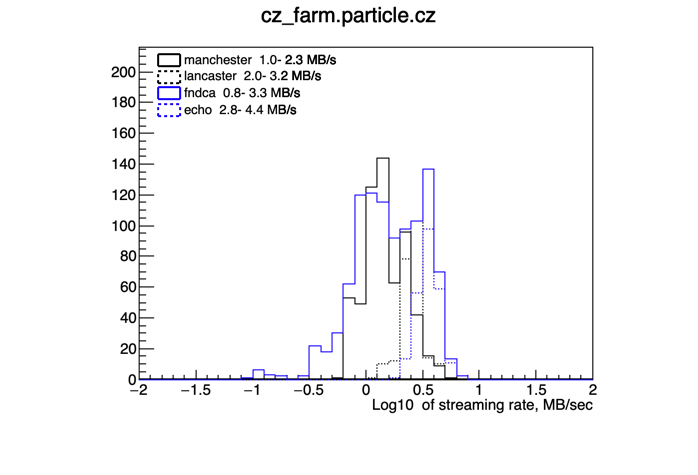
\includegraphics[width=0.45 \textwidth]{graphics/Workflow/dune_fast_2022_01_01_2022_01_07_0_cz_farm.particle.cz.png}
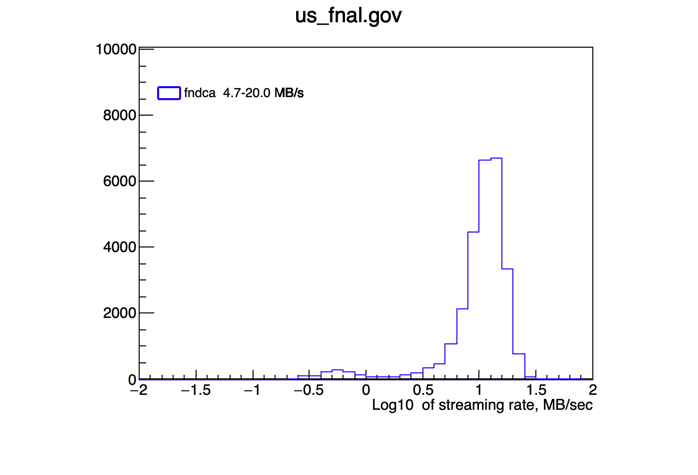
\includegraphics[width=0.45 \textwidth]{graphics/Workflow/dune_fast_2022_01_01_2022_01_07_0_us_fnal.gov.png}
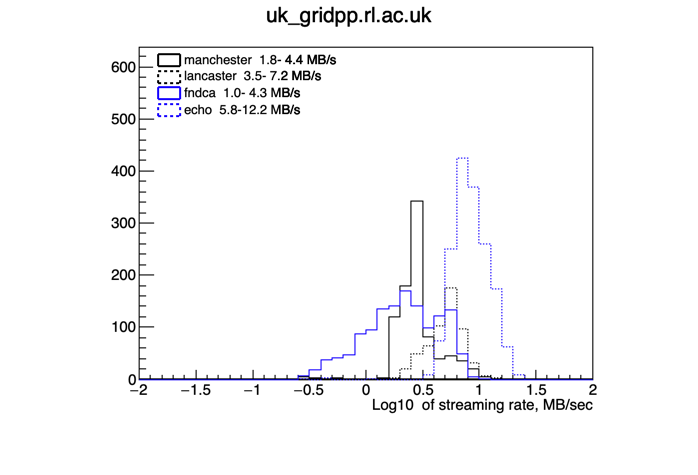
\includegraphics[width=0.45 \textwidth]{graphics/Workflow/dune_fast_2022_01_01_2022_01_07_0_uk_gridpp.rl.ac.uk.png}
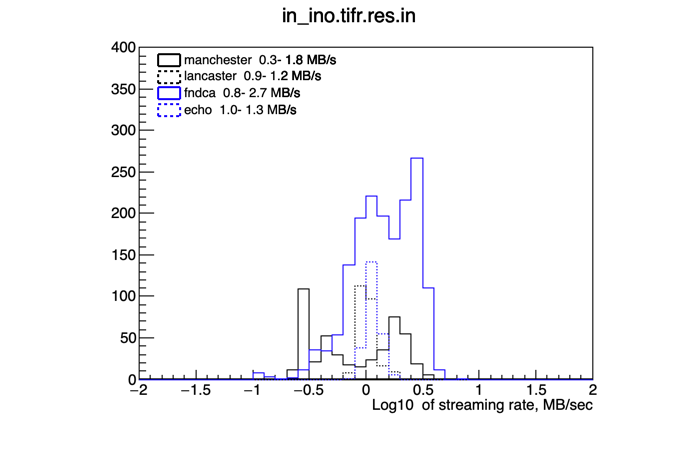
\includegraphics[width=0.45 \textwidth]{graphics/Workflow/dune_fast_2022_01_01_2022_01_07_0_in_ino.tifr.res.in.png}
\end{dunefigure}
%\todo{Get better figure}

\begin{dunefigure}
[Streaming speeds for tuple creation]
{fig:tuplespeedsummary} 
{Streaming speeds for tuple creation jobs running at multiple locations during a test in early January 2022. Reconstructed simulation was stored at sites in the UK and at Fermilab.  The average estimated streaming rates are plotted as a function of disk location ($x$-axis) and compute site ($y$-axis). Jobs in the US were required to use Fermilab disk but international sites were tested with multiple samples.}
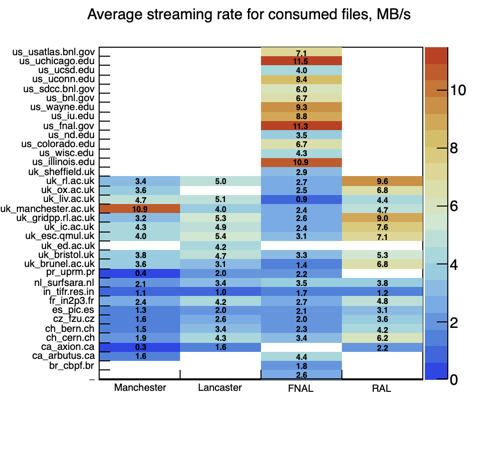
\includegraphics[width=0.8 \textwidth]{graphics/Workflow/fastRates.png}
\end{dunefigure}

\subsection{Implications for Data and Processing Placement}

The current study indicates that for CPU-dominated applications, notably reconstruction of raw data and simulation, the relative location of CPU resources is not critical. Wall time/MB   is similar regardless of location. For IO-dominated applications, proximity to the data is important.  Here there is a trade-off between the availability of resources and the efficiency with which they can be used. Intra-US processing, especially for locations near the national laboratories, is highly efficient, as is processing within the UK.  However, efficiency falls off as the CPU and disks become more separated.  

There are additional constraints imposed on our use of each site at scales greater than that of a single job. Due to local networking limitations, the number of jobs of a particular type we can run may need to be limited to avoid saturating the site's inbound or outbound capacity. 

We have the site information and monitoring tools to provide a workflow management system with the inputs it needs to do optimal placement of data and jobs to maximize efficiency. However our existing data management and workflow tools are not able to take full advantage of this information.  This motivates development of an improved workflow model described below and in Chapter~\ref{ch:wkflow}.



\section{Sites and Services \hideme{McNab - draft}}
\label{sec:cm:sites_and_services}  %% fix label according to section

% Some of this should goes to the Site Resources chapter 
% References to APIs and specific technologies
% perhaps even the definitions types of center and site too

The large \dword{lhc} experiments have historically relied on a tiered structure, with national Tier-1 centers % AM: serving -> and
and regional Tier-2 and Tier-3 centers.  The DUNE model builds on the emergence of faster networks to move to  a service-oriented model, where sites provide services, disk, CPU, real memory/core and archival tape, and projects are  distributed to them based on their capabilities and available networking.  For example, a site with large CPU and memory/core but slower networking would be ideal for simulation while small memory/core and fast access to large local disk stores would be ideal for high-level data analysis.  This model will require a high-level view of data locations and job placement with continual monitoring for bottlenecks, but allows new sites to contribute in an optimal way. The intent is to lower the bar for contributions without overburdening the core computing operations of the experiment.

This section sets out our ``Sites and Services'' model for using sites for DUNE computing tasks, including sites that participate in \dword{osg} or \dword{wlcg} more generally. Since our requirements are not the same as the \dword{lhc} experiments, this %necessitates a distinct naming scheme to 
requires implementing both a distinct naming scheme in
\dword{wlcg} and ways of mapping our scheme onto the \dword{wlcg} tier model.

At this stage, DUNE has chosen to express its requirements in terms of services provided by sites. Each site provides networking plus one or more approved DUNE services, which satisfy DUNE's minimum requirements for the service in terms of capacity, quality, and interfaces. This model allows us to avoid making assumptions about how sites and federations of sites will be organized in the future, as the community evolves away from the strict \dword{wlcg} tiers model towards \dword{doma} and concepts like %a
\dwords{datalake}.
%\todo{define data lakes please. Maybe add to glossary-comp-cdr. } %anne (already said) instead we express our requirements in terms of the services we interact with.

DUNE expects to be able to access services using broadly the same set of APIs as \dword{wlcg} (e.g., HTCondor-CE and \dword{xrootd}) and by using common cloud APIs (e.g., \dword{openstack} and \dword{s3}). 
%kirby - updated Mar 11 \todo{(anne) Should xroot be xrootd? I added the others to glossary-comp-cdr; please fill in the definitions}
For this reason, sites may be operated using conventional grid technologies, on-premises cloud systems, or commercial cloud services. Nevertheless, sites do appear in the DUNE computing model, as the atomic unit for operations activity. %Kirby - fixed Mar 11, 2022 \todo{(anne) This feels like a nonsequitur (and see ??? below)}
For example, staff at a site can receive and process tickets, %may  
and may be required to have a representative at an operations meeting with the technical knowledge to comment on issues as they arise.

In terms of workflows and data management, DUNE does not impose or require any hierarchy or grouping of sites, and assumes that, in general, data may flow between services at any two sites. That said, DUNE expects to use network proximity and bandwidth information to guide the efficient transfers of data between services. The details of the different services within the DUNE Computing Model are described in detail in Section~\ref{sec:cm:types_of_service}.

\section{Sites, Federations, and Countries\hideme{McNab - draft}}
\label{sec:cm:federations}

As well as sites, there are two more administrative concepts: federations and countries.
Federations are borrowed from \dword{wlcg} and represent one or more sites that together pledge a particular amount of capacity to DUNE and enter their pledges into a system like \dword{cric}. %Kirby commented it out since someone did this. \todo{add def to gloss}
Sites may choose to organize themselves this way as it allows more flexibility in how pledges are met against a background of planned upgrades at sites, unplanned outages, etc. 

Countries are represented directly or indirectly at the DUNE Computing Contributions Board, and consist of one or more federations. Broadly, countries map to funding bodies and %are 
provide the entity reviewed when comparing the level of contribution to computing capacity versus the number of DUNE members. %Kirby - Mar 11, 2020 \todo{(anne) please clarify what's being compared, I don't get it. Where do you get number of members?} 




\section{Types of Service\hideme{McNab - draft}}
\label{sec:cm:types_of_service}

We envisage five classes of service on which we will put requirements and request capacity:

\begin{itemize}
    \item Network,
    \item DUNE Computing Element,
    \item Data Cache,
    \item DUNE Storage Element, and
    \item DUNE Data Archive.
\end{itemize}

\subsection{Network\hideme{McNab - draft}}
\label{sec:cm:network}

Networking is needed at all sites, with basic requirements including IPv4 and \dword{ipv6}. %Kirby someone did this \todo{please add to gloss, also NREN below}
All sites should be connected to the wide area network, typically via their \dword{nren}, with sufficient capacity to handle the data IO commensurate with their fraction of the workload. In practice this means at least 40\,Gbit/s for major sites with large amounts of storage (with 100\,Gbit/s becoming the normal expectation for a shared site such as a \dword{wlcg} Tier-1) and at least 20\,Gbit/s for smaller CPU-only sites (but with 40-100\,Gbit/s becoming the norm in shared sites).
Other DUNE-approved services may impose further requirements in terms of network capacity. %anne which they require,

\subsection{DUNE Computing Element\hideme{McNab - draft}}
\label{sec:cm:dce}

A DUNE Computing Element is a service that gives access to jobs consuming CPU. %anne  to perform computation. 
%anne To 
Regarding the operational overhead %anne in working with 
for each site, DUNE will require  minimum standards for

\begin{itemize}
    \item %anne The support level, in terms of whether tickets will be acted 24/7 or only during working hours
    the support level, e.g., 24/7 or only during working hours;
    \item the total number of logical processors across the service;
    \item the interface used to submit jobs or create virtual machines;
    \item the operating system version for grid capacity;
    \item memory and scratch disk space per processor;
    \item incoming and outgoing network capacity per processor; and
    \item %Suitable (already 'min standards for')
    access to a DUNE Storage Element or Data Cache, which allows data intensive jobs to execute without an unacceptably low CPU efficiency.
\end{itemize}

We envisage three subclasses within the computing element services aimed at centrally managed data processing, at user or working group data analysis, and at detector simulation, data cache, DUNE storage element, and DUNE data archive. These subclasses have different requirements for network access, and in the case of data analysis, for support level.

\todo{(anne) I'm taking these out of subsections -- too small.}
%\subsection{Data Cache\hideme{McNab - draft}}
%\label{sec:cm:data_cache}
The data cache, not managed by DUNE systems, requires:
\begin{itemize}
\item suitable networking,
\item sufficient nearby DUNE Compute Element capacity,
\item transparency, and
\item resiliency against transients to prevent jobs from dying and hence data loss.
\end{itemize}

%Suitable networking. Sufficient nearby DUNE Compute Element capacity to be useful. Not managed by DUNE systems. ``Transparent''. Data loss is equivalent to jobs dying, so a transient which DUNE systems will recover from.

%Kirby put this section back in because I think storage element is a first class service.
\subsection{DUNE Storage Element\hideme{McNab - draft}}
\label{sec:cm:dse}

The concept of a DUNE Storage Element mirrors that of a DUNE Compute Element. It must be of sufficient capacity, measured in hundreds of TB or in PB, for the operational overheard to be worthwhile. It must have a suitable support level. %defined above, in terms of whether tickets will be acted 24/7 or only during working hours. 
There must be enough inbound and outbound networking capacity for global data placement operations, and for jobs to write data there or to consume the data already present. In particular, there must be %anne a minimum amount of 
enough DUNE Compute Element capacity available nearby %, on which DUNE jobs can access 
that DUNE jobs can access the storage service % an unacceptably low CPU efficiency. 
while retaining sufficent CPU efficiency.

This formulation allows conventional grid sites with CPU and disk storage mixed together in adjacent racks, and also novel regional architectures such as data lakes %Kirby - done \todo{will be a gloss term!} %in which there is 
with sufficient network capacity to link CPU and storage at different locations. At this stage of the project, DUNE does not want to prejudge what will be available at the start of data taking, and does not want to discourage the exploration of new and more efficient ways of providing resources.

%\subsection{DUNE Data Archive\hideme{McNab - needs work}}

%Kirby - just not really need this sentence. Networking. Cache? Support level? Tape without saying only tape forever. \todo{Anne ignored this!}

%The host laboratory is the most important center and during DUNE data %taking will be FNAL. During protoDUNE data taking, both FNAL and CERN %have host laboratory roles. A host laboratory runs central services %for DUNE, makes the largest single contribution in disk and CPU, and %acts as an archive center and user center. This broadly corresponds %to the WLCG Tier-0 concept. 
%
%Archive centers fulfill DUNE’s requirement to have two copies of raw %data on tape (or other archival-quality storage systems), including %one not at the Host Laboratory. It is not essential that archive %centers also have significant amounts of disk and CPU available to %DUNE as they may only be needed for disaster recovery and for %recovering individual lost files. Amongst WLCG sites, archive centers %would be based on the tape archives of Tier-1s, and the concept maps %directly to the DOMA idea of an archive center where disk storage and %CPU may be absent.
%
%Disk centers provide storage managed by DUNE, along with significant %amounts of CPU, and satisfy DUNE’s requirements for the ratio of CPU %to disk, the bandwidth between CPU and disk, and the bandwidth to and %from other participating centers. DUNE does not require 24/7 on call %support for disk centers, but may use the declared support level when %deciding where to place data and where to direct workflows. Disk %centers correspond to WLCG Tier-1 sites or Tier-2 sites with disk, %and to DOMA Data and Compute Centers.
%
%Compute centers provide only CPU capacity, scratch disk associated %with jobs running on worker nodes for the duration of jobs, and %possibly transparent caching (eg Xcache). That is, they do not %provide storage which is managed by DUNE. They do however satisfy %DUNE’s requirements for bandwidth to and from other participating %centers. Compute centers correspond to WLCG Tier-2 sites without %disk, and to DOMA compute centers. 
%
%User centers are used for end user analysis, by people submitting %jobs and managing workflows, and may need to download or stream a %limited amount of data directly from disk centers.
%
%
%
%\section{Requirements for Computing Services \hideme{McNab - needs %work}}
%
%What we need DUNE services to be able to do, to do the above.
%
%
%\todo{consider both cases of data to job and job to data - discuss %current issues but be vague about the future}
%
%%%%%%%%%%% notes from 10-29

% Define a minimal "CPU-only" service

% Define a DUNE-managed disk service - how many TB min - requires support. 

% Define a tape service

% Mention possible need for cache for 

%(How do they get the code? cvmfs or container.  

%\todo{Andrew compares the use case footprint table into a sites %comparison}
\end{document}
\cleardoublepage

\chapter{Site Resources - (McNab)}
\label{ch:sites}

%%%%%%%%%%%%%%%%%%%%%%%%%%%%%%%%
\section{xyz}
\label{sec:sites:xyz}  %% fix label according to section

\cleardoublepage

\documentclass[../main-v1.tex]{subfiles}
\begin{document}
\chapter{Data Placement \hideme{Steve, Kirby and Heidi } }
\label{ch:place}

%%%%%%%%%%%%%%%%%%%%%%%%%%%%%%%%
%\section{xyz}
%\label{sec:places:xyz}  %% fix label according to section

\section{Current Status}

DUNE relies on a multi-level data placement strategy that has grown out of the Fermilab fixed target program with elements from CERN fixed target experiments.  Figure \ref{fig:storage} illustrates the storage available to users. Reference \cite{bib:storage} provides a more detailed description. 

\subsection{Storage systems at Fermilab}

There are two general use cases considered for storage systems at Fermilab: production operations and analysis end users. Production operations is in general focused on utilization of large-scale storage elements. Analysis end users though utilize a wide variety of storage systems and typically log into on of a set of \dwords{vm}  which have disk mounts of varying size and level of backup. 

\begin{description}

    \item{\bf Local disk -}  There are small   volumes on local physical disks, directly
mounted on the machine hosting the \dword{vm} with direct links to the /dev/ location
used as temporary storage for infrastructure services (e.g. /var, /tmp).
These areas should be used to store certificates and tickets. These secure items are saved to local disk automatically with owner-read permission and other permissions disabled.
These local areas are usually very small and should not be used to store data files or for code development.
    
    \item{\bf Network Attached Storage}
    
     Users have access to POSIX compliant network attached storage areas with varying sizes and levels of backup. Network attached disks are not safe for storage of certificates and tickets.

 \begin{itemize} 
   \item Users are provided with a network mounted home area {\tt /nashome/} (usually 2 GB).    A valid Kerberos ticket is needed   to access files in the home area. Periodic snapshots are taken and available in "{\tt  /nashome/.snapshot}". There are additional network mounted areas for code development and small data analysis samples. 
\item {\tt /dune/app} is intended for code development and is  limited to 100 GB/user.  /dune/app has periodic snapshots in /dune/app/.snapshot

\item  {\tt /dune/data} and {\tt /dune/data2} are larger areas for fast analysis and code testing.  They are not backed up.  
\end{itemize}
 
The \dword{nas} disks {\tt /dune/app} and {\tt /dune/data} are not accessible as an output location from grid worker nodes. 
 
\item{\bf dCache -} Several PB of \dword{dcache}\cite{Millar:2014cfa} storage is available at several scales. \dword{dcache} storage is not fully POSIX compliant but \dword{nfs} mounts with limited functionality are available on Fermilab interactive machines. The \dword{dcache} storage is readable and writable from grid machines via \dword{xrootd} and transfer mechanisms such as \dword{ifdh}. It is expected that this is the main storage element for the output of both production and analysis distributed computing jobs.

\begin{itemize}
    \item {\tt /pnfs/dune/scratch}  is a scratch area used mainly for files returning from grid jobs.  Files are automatically removed to accommodate new files. Typical lifetimes are 1 month. 
     \item {\tt /pnfs/dune/persistent} is a $\approx 800$ TB area for persistent storage of user files.  Files must be removed by their owner. Half of this volume is currently controlled with physics group based quotas, while the other half will soon be trainsitioned to quota-controlled usage.
      \item {\tt /pnfs/dune/tape\_backed} is a $\sim 3.2$ PB disk cache sitting in front of the \dword{enstore} tape system. Files in this area are cataloged and tracked by the \dword{sam} system and, in future, by \dword{rucio}. Users may need to prestage samples to make them rapidly accessible. 
\end{itemize}
\item{\bf Distributed caching systems - } \dword{dune} makes use of the \dword{cvmfs} caching system to distribute code, flux and shower libraries and user grid executables. \dword{cvmfs} mounts are available on DUNE grid nodes. 



\begin{itemize}
    \item {\tt /cvmfs/ } mounts of DUNE-specific code,  shared executables such as \dword{larsoft}, and general utilities are distributed via \dword{cvmfs}. Version control is provided by the Fermilab \dword{ups} system. 
    
    \item \dword{stashcache} is used to deliver larger payloads such as flux files and shower libraries to grid jobs.
    
    \item A \dword{cvmfs}-based  {\tt dropbox} is also available to transfer user executables to grid jobs. 
    
    



\item{Collaboration disk stores}
DUNE collaborating institutions also contribute very substantial storage resources. These resources are populated and managed via \dword{rucio} and currently accessible via the \dword{sam} catalog. As with the Fermilab \dword{dcache} stores they are available via streaming and grid-copy mechanisms but are not mounted on interactive nodes. 
 \end{itemize}


\end{description}
\begin{dunefigure}
[Storage Schematic]
{fig:storage}
{Storage systems for DUNE computing.  Thick lines denote mounts while thinner lines denote transfer methods such as ifdc and xroot streaming.}
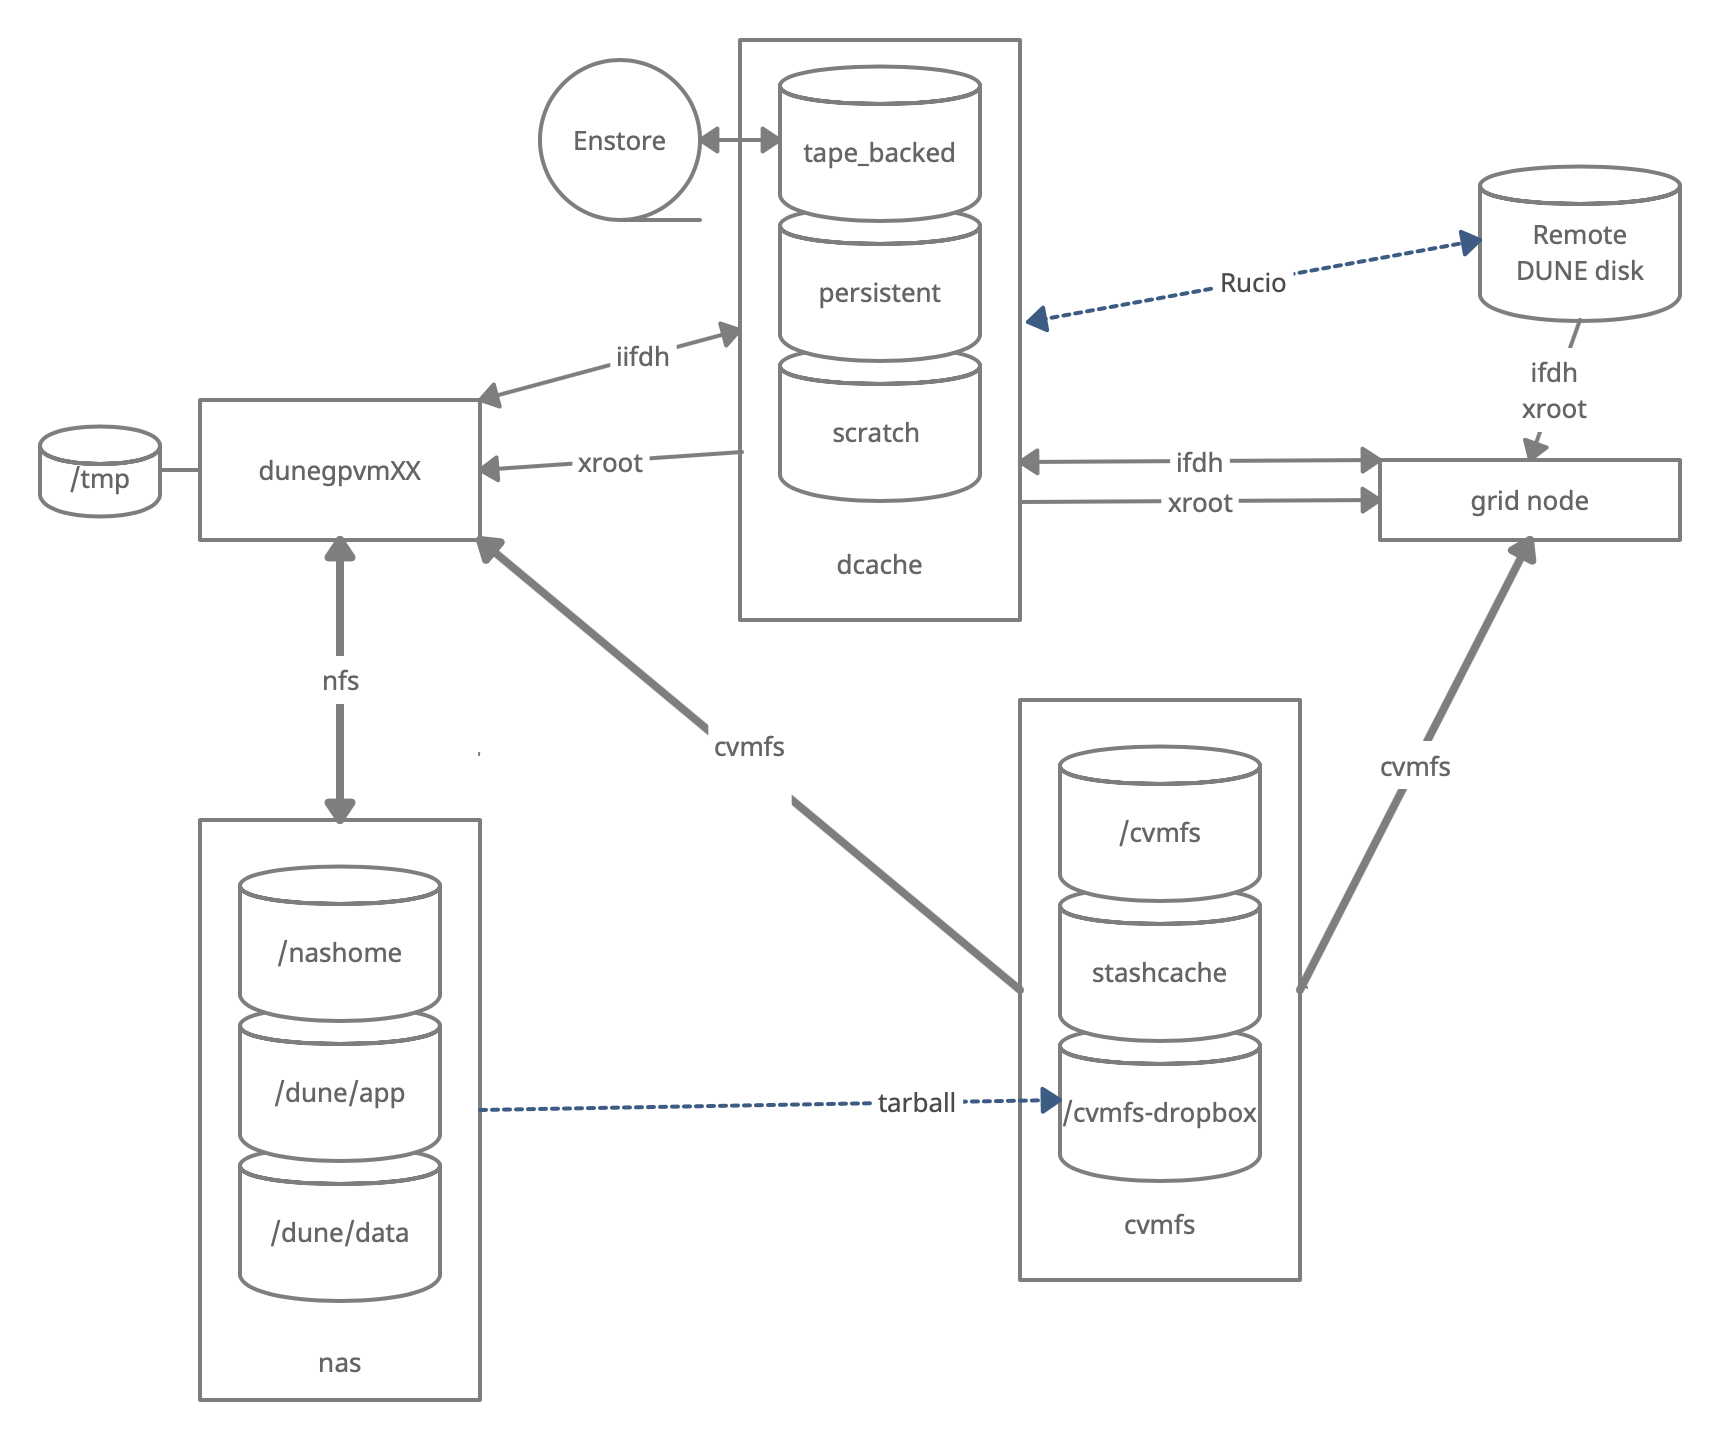
\includegraphics[width=0.8\textwidth]{graphics/DataManagement/StorageMap2.png}
\end{dunefigure}

\section{Storage systems at CERN}

Data at CERN are stored in the \dword{eos}, \dword{castor}, and \dword{cta} systems.  Some of this storage is under the control of the \dword{dune} \dword{rucio}
system, including a full copy of the \dword{protodune} raw data in \dword{castor}/\dword{cta}.  There is also substantial space for generic use by CERN-based users. The \dword{cvmfs} file systems are mounted at \dword{cern} and local users have access to the \dword{cern} batch resources through the normal \dword{dune} batch system which requires membership in the \dword{dune} \dword{vo} and through normal \dword{cern} submission systems.  

\section{Data Placement Strategy}

%Kirby this looks to me like it's done. \todo{What is our data placement policy and how is it implemented in the compute model. }

%\section{Data Placement Strategy}
%The following items describe the placement strategy that DUNE is utilizing to distributed the data globally:
%\begin{itemize}
%\item all \dword{dune} and \dword{pd} raw data to be located at two archival storage elements
%\item all production datasets to be stored on at least one archival storage element
%\item all production datasets will be actively located on at least two storage elements that are geographically separated by an ocean
%\item replication and distribution of raw data and production datasets will be implemented and performed by Rucio
%\item all datasets will have a well-defined data lifetime within the Rucio system
%\end{itemize}

\dword{dune} data has a large number of data access patterns based on the size, CPU/byte and frequency of access.   Major examples are:

\begin{description}
    \item{\bf Raw data -}  Raw data from the TPC detectors comes in 4-8 GB files which are generally run through reconstruction algorithms that take of order 5-10 sec/MB to process. Raw data is generally accessed a few times for calibration and reconstruction as part of an organized production effort.  
    \item{\bf Reconstructed data -}  Reconstructed data from \dword{pdsp} is around three times smaller  than the raw data once the raw TPC waveforms are dropped. It is accessed many times by end users for algorithm development, calibration and production of physics analysis samples.   Observed data access rates range from 1 to 40 MB/sec depending on the amount of reprocessing done to data. 
    \item{\bf Simulated data - } Simulated data are around twice as large as real data due to the large amount of simulation information that is kept.  Even after raw waveforms are dropped, records are still significantly larger. 
    \item{\bf Analysis samples - } End-user analysis samples are significantly smaller.  For example the 1 GeV ProtoDUNE simulation sample consists of $\sim$80,000 4 GB files while the reduced analysis sample is around 8 GB total.  
    \item{\bf Flux files - } Simulation and cross section extraction require access to large libraries of particle fluxes.  These are currently delivered via \dword{stashcache}. 
    
\end{description}

As described in the data volumes section \ref{ch:est}, raw data is kept in multiple tape copies but only kept on disk for the short period before calibration and reconstruction are complete.  If reprocessing is needed, the raw data must be prestaged to cache and work on optimizing this process is underway. Recent reconstructed data and simulation copies for users are kept on \dword{rucio}/\dword{sam} controlled disk, with one copy in the US and one in Europe if possible. Smaller final analysis samples are kept on user or group controlled persistent dcache or \dword{nas} areas. aAl datasets will have a well-defined data lifetime within the Rucio system and replication and distribution of raw data and production datasets will be implemented and performed by Rucio.

%\todo{Overlay policy - how does it work for MicroBooNE and NOvA}
\end{document}




\cleardoublepage

\chapter{Networking \hideme{Mike Kirby and Peter Clarke}}
\label{ch:netw}

%%%%%%%%%%%%%%%%%%%%%%%%%%%%%%%%
%\section{xyz}
%\label{sec:netw:xyz}  %% fix label according to section


\todo{{\it }Kirby to write first about US side of the network including 
- US OSG site connectivity 
- FNAL connection to ESNET
Pete then hooks Europe on to this.}

\todo{Some of this may move into cooperation section}

Connection to European sites is accomplished via ESNET peering with Geant.  
ESNET provides redundant transatlantic links at xxxx Gbit/s. These peer with Geant in ???London??? and ???Amsterdam??.
Geant is the EU wide research network with a core capacity of several hundred Gbits/s. Geant in turn peers with NRENS (National Research and Education Networks) in each participating country, although details pertaining to each DUNE site vary. As example, in the UK the NREN is JISC-JANET, which at the time of writing has a 400 Gbit/s core and connects to the GridPP-RAL site redundantly at 100 Gbits/s. 
Similarly CC-IN2P3 site in France is connected to RENATER at 100 Gbits/s, and the FZU site in the Czech Republic is connected to CESNET at 100 Gbit/s Gbit/s.  DUNE expects all participating countries to ensure that as part of their pledges of CPU and storage capacity, that the sites offered have commensurate network connections. We do not expect any systematic issues to arise, and none have done so in the WLCG/LHC context. DUNE participates in the worldwide HEP Network coordination body.

In respect of layer-3 VRF provision (Virtual Routing and Forwarding), use of this technology is now very prevalent in HEP. VRFs provide a logical routing overlay that can allow for traffic engineering to utilise high capacity paths where needed. The LHC community uses a VRF called LHCONE, and this has also been used for DUNE traffic along with other non-LHC experiments such as BELLE. 
At present DUNE is agnostic to the use of LHCONE, and since FNAL is connected to LHCONE it can easily accommodate sites with or without such provision.
Investigations are currently underway to determine the technical requirements for the creation of a separate DUNEONE VRF were it to ever be required. It is however not currently foreseen, and does not form part of our baseline planning.
\cleardoublepage

\documentclass[../main-v1.tex]{subfiles}
\begin{document}
\chapter{Workflow Examples \hideme{Herner, Timm, McNab - needed}}
\label{ch:wkex}
\hideme{combine into workflow}
%%%%%%%%%%%%%%%%%%%%%%%%%%%%%%%%
%\section{xyz}
%\label{sec:wkex:xyz}  %% fix label according to section

\todo{diagram of simulation workflow from POMS}
\end{document}
\cleardoublepage

\part{Computing Services (Steve Timm)} % Timm

\chapter{Services Overview \hideme{Timm}}
\label{ch:serv}

%%%%%%%%%%%%%%%%%%%%%%%%%%%%%%%%
%\section{xyz}
%\label{sec:serv:xyz}  %% fix label according to section
\section{Introduction}
DUNE computing is dependent on a number of services that are not operated by DUNE itself.
Some of these are provided by the host lab, others are provided by the various remote sites where
computing is done, and still others are operated by commercial companies and hosted in the cloud.

\section{Host Lab Provided Services}
\section{Remote Site Provided Services}
\section{Cloud Hosted Services}

\todo{section on assumptions about external services that we depend on}
\cleardoublepage

\chapter{Data Management \hideme{Steve Timm and Robert Illingworth} }
\label{ch:datamgmt}

%%%%%%%%%%%%%%%%%%%%%%%%%%%%%%%%
\section{Introduction}
\label{sec:datamgmt:xyz}  %% fix label according to section

The Data Management subsystem serves the function of bringing data from the detectors to the archival storage facility 
and then distributing it to storage elements around the world.  The components include a data ingest manager, a
replica manager that knows the location of files and manages the transfers between storage element, a metadata 
catalog that keeps track of the types and provenance of data, and an interface to deliver the appropriate files 
to the workflow management system and interactive users.

DUNE Data Management is currently in the process of deploying several new components in the Data Management
system, to replace the legacy SAM system which currently does the function of replica manager, metadata server, 
and file delivery.  The goal is to have the new system in place before beam running begins on ProtoDUNE-II
(single-phase horizontal drift).  

\todo{Need to insert basic data management architecture here}

\begin{figure}[ht]
    \centering
%\includegraphics[height=6cm]{graphics/DataManagement/Figures/data_management_diagram.pdf}
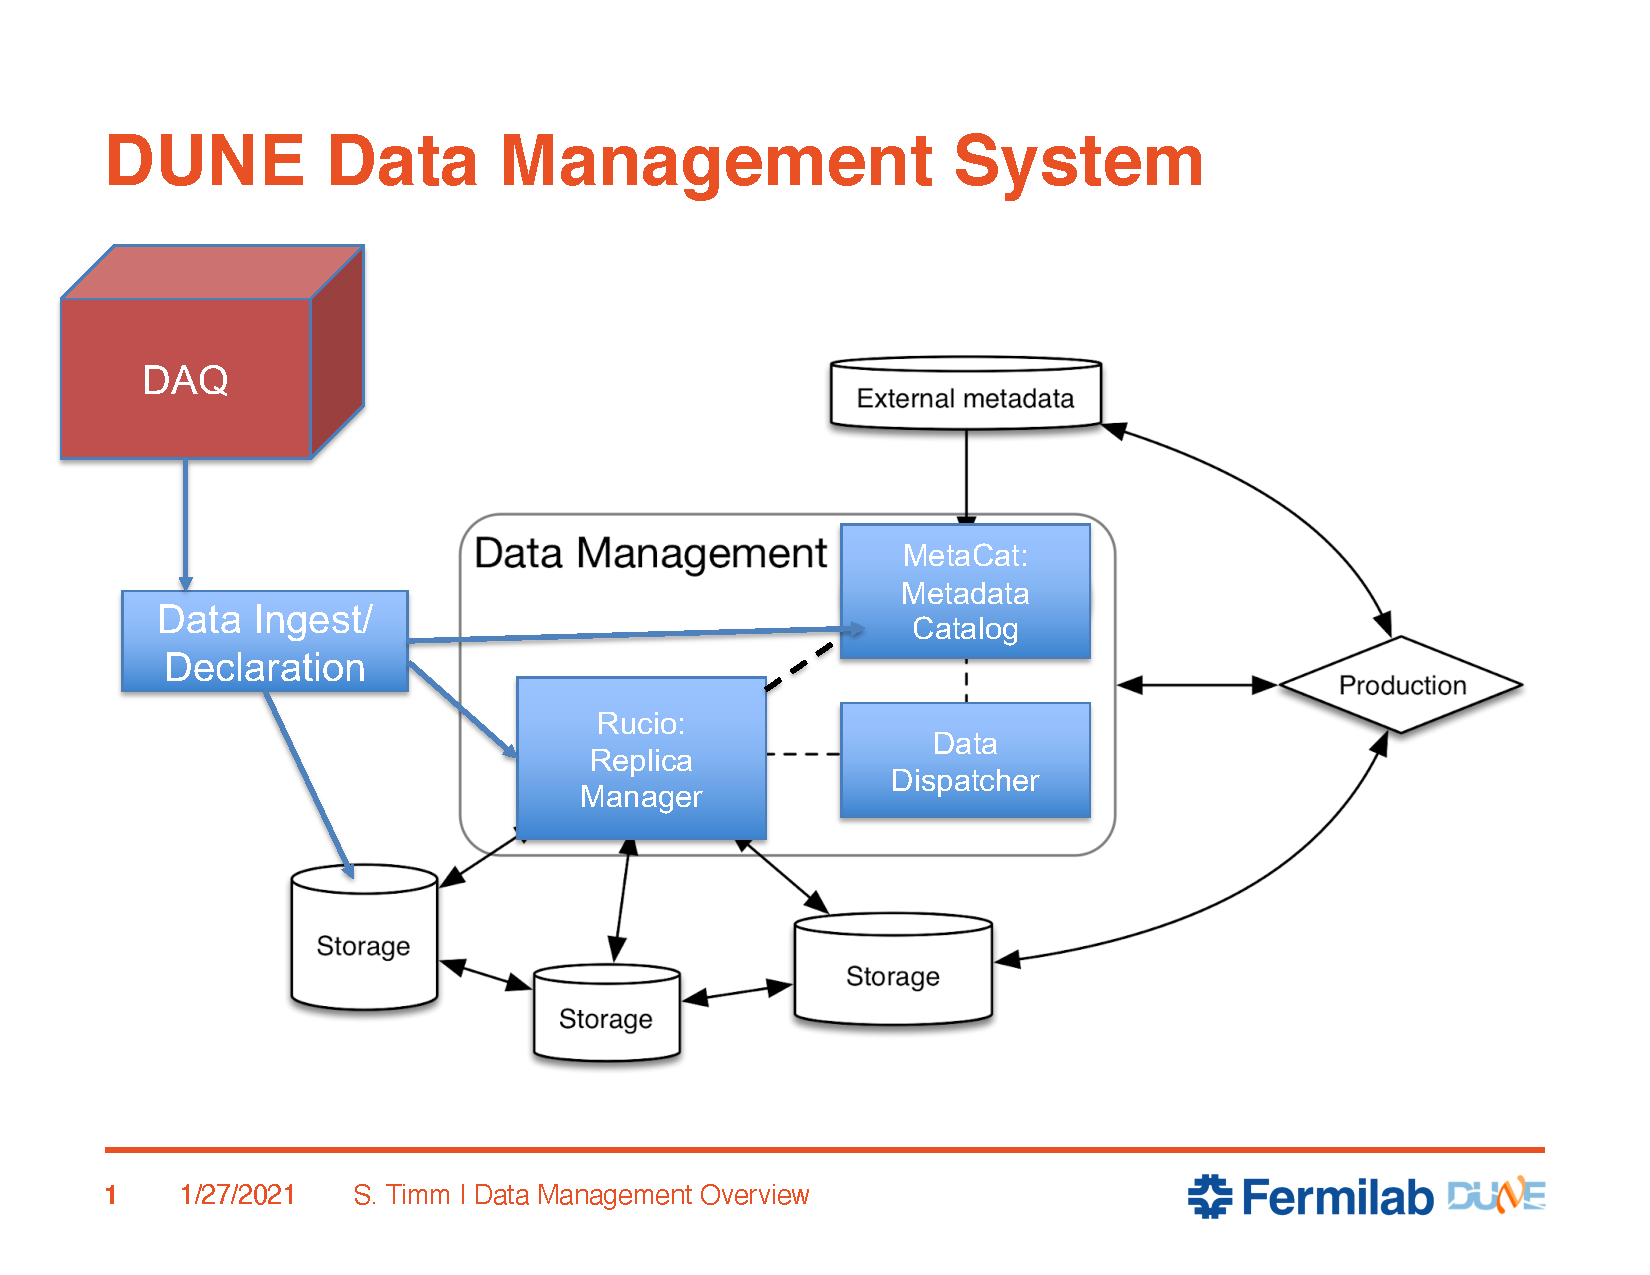
\includegraphics[height=8cm]{graphics/DataManagement/data_mgmt_diagram.pdf}
    \caption{Data Management Architecture Diagram}
    \label{fig:datamanagement}
\end{figure}


\section{Data Ingest Manager}

The Data Ingest Manager will run at detector sites.  It consists of two components:  the Ingest Daemon and the Declaration Daemon.  The Ingest Daemon will 
run within the detector hall, detect new files in the data store, extract the metadata and add new metadata fields
if necessary, calculate the checksum of the files, initiate and monitor the transfers to the first managed 
storage element, and send a signal back to the DAQ when the file has been transferred and can be deleted from the data store.
Files will be transferred to a dropbox on the nearest managed storage element, using FTS3 as the transport mechanism.  
The Declaration Daemon will run on or near a storage element that is managed by the replica manager. 
It will detect new files that have been added to the dropbox, and declare them to the metadata catalog and the replica manager.  It will then instruct the replica manager to send these files to permanent tape-backed storage and monitor the transfer to be sure that this has been done, and then send a signal to remove them from the temporary dropbox.

These daemons will be performing most of the functions that the current data transport system does, they only 
require modification to contact the new replica manager and metadata catalog rather than the current ones.  The 
requirements for these daemons have been defined and we expect coding work to start in mid to late summer 2021.

\section{Replica Manager}

The replica manager has the functionality of tracking where all data files are located and ensuring that they 
are moved from point to point as needed.  The choice that we have made for this functionality is the Rucio data
management system.  This system was originally developed by the ATLAS experiment and has now been deployed to 
a number of other HEP and astronomy experiments.  DUNE has had a Rucio server since 2019.  All raw data that was
taken in the fall 2018 ProtoDUNE-SP (NP04) run and since that time, as well as all raw data taken by the ProtoDUNE-DP (NP02) run, is tracked by Rucio.

Rucio is a rule-based system.  Files are sent to remote servers and kept there based on a system of rules
that are created by the experiment data managers.  Data can be accessed interactively or in batch jobs and
Rucio has a built-in system of delivering the URI of the closest replica to the running job for access via streaming.

The main work that remains to be done in implementing the Rucio server is the process of back-loading all relevant 
data in the legacy SAM system into Rucio as well.  Currently about 50\% of the data by volume is known by Rucio but only about 25\% of the files by file count are declared to Rucio at the moment.  This is the largest current 
operational issue under way.

There are also some key features that we need from the Rucio developers.  One of them is the capacity to 
do the logical to physical file name mapping on our tape sites, based on the metadata of the file.  Another
is the hook that requires that any file that is declared to Rucio is also declared to the metadata catalog.

Rucio has a rudimentary internal metadata functionality but it is not used by any of the main 
experiments that use it.  We thought it wise for DUNE to also have a 
\section{Metadata Catalog}



\section{Data Dispatcher}

\section{Tools}



\cleardoublepage

\documentclass[../main-v1.tex]{subfiles}
\begin{document}\chapter{Workload Management  - \hideme{Ken Herner - needed - merged into workflow }}
\label{ch:wkload }
\hideme{workload merged into workflow chapter}
%%%%%%%%%%%%%%%%%%%%%%%%%%%%%%%%
%\section{xyz}
%\label{sec:wkload:xyz}  %% fix label according to section


%\todo{describe POMS}
\end{document}
\cleardoublepage

\chapter{Workflow Management \hideme{future}}
\label{ch:flow}

%%%%%%%%%%%%%%%%%%%%%%%%%%%%%%%%
%\section{xyz}
%\label{sec:flow:xyz}  %% fix label according to section

\cleardoublepage

\documentclass[../main-v1.tex]{subfiles}
\begin{document}
\chapter{Information Systems \hideme{McNab}}
\label{ch:is}

DUNE intends to use \dword{cric} \fixme{dword needs def} as a central source of information about sites and their compute and storage services. \dword{cric} is routinely used by ATLAS and CMS with \dword{osg} and other \dword{wlcg} resources, and is also familiar to site administrators. 

An evaluation of \dword{cric} is being done, with information about sites obtained from the configurations of the \dword{osg} pilot factories. This is browsable via the \dword{cric} web dashboard, and also used to generate XML files in the \dword{vo} Feed format required by the \dword{etf} testing framework used for monitoring.
% ref to chapter for this



%%%%%%%%%%%%%%%%%%%%%%%%%%%%%%%%
%\section{xyz}
%\label{sec:is:xyz}  %% fix label according to section
\end{document}
\cleardoublepage

\documentclass[../main-v1.tex]{subfiles}
\begin{document}
\chapter{Monitoring \hideme{ Steve Timm, Raja Nandakumar, Jon Hays - in progress}}
\label{ch:mon}

% Create Parameter Values - most #'s will need to be handled this way
% Preface parameter name with the chapter tag
%%%%%%%%%%%%%%%%%%%%%%%%%%%%%%%%
\FPset{MonEtfOpsPeople}{3.1} % FTE
\FPset{MonEtfDevPeople}{1.0} % FTE
\FPadd\MonEtfTotalPeople\MonEtfOpsPeople\MonEtfDevPeople %FTE

This section %anne concerns 
describes the monitoring of services and resources on the grid. % anne The actual monitoring of the jobs that are submitted by DUNE 
Monitoring of DUNE jobs (\dword{wmsmon}) is covered elsewhere. \fixme{(anne); add def to wmsmon and find "elsewhere" and reference} As the workflows are broadly similar to current \dword{lhc} experiment workflows, DUNE plans to reuse the relevant monitoring tools (\dword{etf}, \dword{perfsonar}) developed for this purpose by the \dword{wlcg}. %anne, which we cover in this section.
These tools are described here. 

%Going forward, DUNE plans to be agile and keep up with upcoming developments in this field. If there is a paradigm change in the resources made available, there may be a need to develop new tools to keep on top of the available resources and display them in a transparent manner. An example can be the widespread deployment of ipv6\cite{bib:ipv6TaskForce} networking requiring possible re-evaluation of various tools for computing. The ETF and perfSonar tools are already ipv6 compatible and can be deployed to test resources offering ipv6 connectivity in either pure or dual-stack mode.
Going forward, DUNE plans to be agile, keep up with upcoming developments in this field, and develop new tools as needed. For example, the widespread deployment of \dword{ipv6}~\cite{bib:ipv6TaskForce} networking may require re-evaluation of some of our computing tools.  The \dword{etf} and \dword{perfsonar} tools are already \dword{ipv6} compatible and can be deployed to test resources offering \dword{ipv6} connectivity in either pure or dual-stack mode.

%%%%%%%%%%%%%%%%%%%%%%%%%%%%%%%%
\section{Tools}
% \begin{dunetable}
% [Monitoring Assumptions]
% {l r l}
% {tab:mon:assumptions}
% {Assumptions for Monitoring}
% Parameter&Value&Comment\\
% ETF personnel&\etfPeople&no comment\\
% \end{dunetable}
\label{sec:mon:xyz}  %% fixhttps://www.overleaf.com/project/5f5a7bb23f29aa0001f211d2 label according to section
\subsection{Experiment Test Framework (ETF)}

DUNE jobs \fixme{may?} run on all sites on the grid. Checking the status of these jobs is one way of keeping an eye on whether a given site or resource is functioning normally. Given that issues can and usually do have multiple sources, it is essential to have an independent resource monitoring system to %anne keep an eye on what is happening to help 
catch issues quickly. %The framework that is being successfully used for this is \dword{etf}. %, is already in the \dword{wlcg}. % WLCG is the ETF system.
\dword{etf}, framework that is being successfully used for this, is the \dword{wlcg} % WLCG is the ETF system.
 Experiments Tests Framework\cite{bib:ETFDoc},\cite{bib:ETFStatus}. It  has been known by different names, but the underlying framework remains the same. The \dword{cern} plans to support this framework for as long as \dword{lhc} experiments require availability and reliability metrics from an independent source.
 
\dword{etf} is a system of tools that regularly test all the available resources for different experiments, i.e., \dwords{vo}. It has been developed and run on behalf of the \dword{wlcg} %anne experiments (VOs) 
 \dwords{vo} for well over a decade. % now. 
% This framework supports each \dword{vo} running tests customized to the application and systems required by the VOs to enable a true picture (availability, reliability) of the resources available for the VO. The ETF tests run hourly and feed into the MONIT framework which keeps history information and the most recent test logs for enabling debugging and metric measurement.
This framework runs tests customized to the \dword{vo}'s application and systems to provide a true picture of the  available resources and their reliability. The \dword{etf} tests run hourly and feed into the \dword{monit} \fixme{add dword def}
framework, which keeps history information and the most recent test logs to enable debugging and metric measurement.

The \dword{etf} framework currently involves 
\begin{enumerate}
\item high-level functional testing of about 90 hosts defined in the \dword{glideinwms} configuraton;
\item dashboard (checkmk) to show results; and
\item plugins conforming to Nagios\footnote{Nagios\textregistered, \url{https://www.nagios.com/}} standard. 
\end{enumerate}

%anne moved up and edited. The framework has been named differently over the years keeping the underlying framework the same. With WLCG based at CERN as it is aimed for the LHC VOs, CERN currently plans to support this framework for as long as LHC exists as there will always be a need for availability and reliability metrics from an independent source.

\begin{comment} see below (anne)
Some customization of the tests has been done, and  further changes being planned, which are :
\begin{enumerate}
    \item Minimal simulation to test that a simulation works on the worker nodes (Done)
    \item Checking if a given worker node has ipv6 networking (Done)
    \item Lightweight test of access to rucio servers from the worker node (ongoing)
\end{enumerate}
\end{comment}

Customized tests are in place to verify %that a minimal simulation works 
a minimal simulation functionality on the worker nodes and to check that a given worker node has \dword{ipv6} networking. A customization to perform a lightweight test of access to  \dword{rucio} servers from the worker node is in progress.

Beyond this, DUNE-specific development will be required from time to time %in keeping 
to synchronize with updates to the framework both from the \dword{etf} / \dword{monit} and the DUNE software ends. %Depending on the requirements we estimate  with 1 
We estimate that this effort will require  one FTE staff. %will be needed.

It is expected that \fixme{X} virtual machines with minimum spec \fixme{X} will be required to run the \dword{etf} service, which can be located at any site (e.g., \dword{cern}).

%anne It is expected a
Another three FTE will likely be required to monitor the \dword{etf} results, probably as part of more general computing shifts. This will involve looking at the test results, following up on failing tests and opening tickets for failing resources. Site administrators can also use \dword{etf} tests to understand the performance of their sites. %anne: seems like it says the same thing -- and it can be used (as it is for the LHC VOs) to provide a measure of site performance (availability, reliability).

See Table~\ref{tab:mon:assumptions} for a summary. 

\subsection{PerfSonar}

%The core part of DUNE (as with LHC experiments) is to distribute the data taken at the detectors to the different resource centers for analysis. This depends on high-performance networking between the sites providing storage. From experience, identifying and solving issues needs detailed debugging tools. The WLCG solution for this is to develop and deploy a pervasive network monitoring infrastructure to identify and debug issues when they occur.
It is critical to distribute the detector data to the different sites for analysis and storage. This requires both high-performance networking between the sites and sophisticated debugging tools to identify and solve problems that arise. The \dword{wlcg} network monitoring and debugging infrastructure that DUNE will adopt and deploy is \dword{perfsonar}.

\Dword{perfsonar} is an open source toolkit collaboratively developed by %multiple 
groups in Europe and the Americas that keeps a clean separation between network-related and other metrics. %This toolkit 
It is installed on dedicated hardware (\dword{perfsonar} boxes) at %all the sites providing resources to avoid contamination of network metrics with other issues.
each resource site. % that provides resources. 
The data from these \dword{perfsonar} boxes %is 
can be aggregated by a variety of tools and algorithms to %see 
visualize the connectivity in different ways, as described in the following web pages: %anne  in various (kibana, grafana, checkmk, ...) ways, enumerated below.
\fixme{ideally we'd make these each references and cite them. (anne)}
\begin{enumerate}
    \item \url{https://psetf.opensciencegrid.org/etf/check_mk/index.py}
    \item \url{https://toolkitinfo.opensciencegrid.org/}
    \item \url{https://monit-grafana-open.cern.ch/}
    \item \url{https://atlas-kibana.mwt2.org/s/networking/app/dashboards}
    \item \url{https://perfsonar.uc.ssl-hep.org/}
    \item \url{https://sand-ci.org}
\end{enumerate}

These tools are currently well supported within \dword{wlcg} with %wide expertise being shared between administrators in various regular meetings and conferences. 
expertise shared widely and regularly among administrators.
Given %the expectation 
that networking is a core need for \dword{wlcg} as it is for DUNE, it is anticipated that \dword{perfsonar} %as a network monitoring and debugging tool 
will continue to be supported %into the future.
as long as DUNE requires it.

See Table~\ref{mon:ops:needs} for a summary.

% \section{Summary of Assumptions and Resources}
% \subsection{Assumptions}

% ETF support assumption reference

% \subsection{Development needs}

% ETF dev effort, N FTE

% \subsection{Compute resource needs}

% ETF resource requirements list

% \subsection{Operations needs}

% ETF ops effort, M FTE



\section{Summary of Assumptions and Resource Requirements}

% This section needs summary tables at the end which will be rolled up for the full document
% Please replace #'s in the text with defined parameters and use those in the table (and teXt)
% Place your parameters at the top of the section. 
%


\begin{dunetable}
[Monitoring Assumptions]%{}
{llrlll}
{tab:mon:assumptions}
{Assumptions for monitoring}
System&Parameter&Value&Units&Comment\\
FD & Cosmic rate & 5000 & per day&\\
%ETF personnel&\etfOpsPeople&no comment\\
\end{dunetable}
\fixme{(anne) fill in the above table? }



\begin{dunetable}
[Resource requirements for monitoring]
{llrlll}
{mon:ops:needs}
{Resource requirements for monitoring}
  System & Resource & Value & Units & Timeline&  Comment\\ \toprowrule   
  ETF Operations & Personnel &\MonEtfOpsPeople  & FTE & 2027-2040&\\ %\colhline % mon-ops-ETF
 ETF Development  & Personnel &\MonEtfDevPeople  & FTE & 2021-2025& \\ %\colhline % mon-dev-ETF
 ETF Total  & Personnel &\num[round-mode=places,round-precision=1]{\MonEtfTotalPeople}  & FTE & 2021-2025& \\ %\colhline % mon-tot-ETF
      & Storage  &3  & GB&2021-2040& \\ 
      \colhline % Start new section
  PerfSonar & Operations &0.1 & FTE &\\ \colhline % mon-ops-PerSonar
  Row 3 & \daqsamplerate & \\ 
\end{dunetable}
\fixme{fix last row of table}
\end{document}
\cleardoublepage

\documentclass[../main-v1.tex]{subfiles}
\begin{document}
\chapter{Code Management \hideme{Tom Junk, Mathew Muether, David Adams - draft}}
\label{ch:codemgmt}

\fixme{Doug: ND-LAr TMS and ND-GAr code management sections need to be written, references for CVMFS and Spack need to be found (anne 3/8: dword for cvmfs, spack footnote in prev chap)}

%%%%%%%%%%%%%%%%%%%%%%%%%%%%%%%%
\section{Liquid Argon TPC Code Management \hideme{Junk/Calcutt - needs update}}
\label{sec:codemgmt:dunetpc}  %% fix label according to section

Software for simulation, data read-in, and reconstruction shares significant commonality across the %anne liquid-argon time projection chamber detectors 
DUNE \dwords{lartpc}. %anne planned to be deployed by DUNE and also  prototypes.  
These comprise the %anne horizontal- and vertical-drift far detector modules, the 35-ton prototype, ProtoDUNE-SP, ProtoDUNE-DP, ProtoDUNE-2, ProtoDUNE-VD, ICEBERG, 
the \dword{sphd} and \dword{spvd} \dwords{detmodule}, the \dword{35t}, \dword{pdsp}, \dword{pddp}, \dword{protodune2},  the pixel \dword{nd} and its prototypes.  The same software stack handles the wire readout, the photon detectors, and the cosmic-ray taggers used in some of the prototypes.  The interfaces to event generators, GEANT4, {\it art} and the data handling systems require effort to build and maintain.  Data products need to be thought out carefully.  To reduce the development burden and expand the pool of expertise, DUNE has chosen to use the LArSoft toolkit, which is built on NuTools and {\it art}.  

LArSoft itself is split up into several repositories, such as larcore, larsim, larevt, lardata, and variations that have been split from them over time, such as lardataobj.  LArSoft is supported by Fermilab's Scientific Computing Division and is shared among several other experiments, such as ArgoNeuT, MicroBooNE, ICARUS and SBND.  The pool of developers is quite large, and the rate at which new code is added is quite significant.  New releases of LArSoft are made weekly.  

DUNE's LArSoft-based software historically had been collected in a single git repository called dunetpc, starting in the early days of the collaboration.  This repository was hosted using Fermilab's Redmine service.  Compiling all of the code in this single repository became slower as more source files were added.  In January 2022, a split of the dunetpc repository into ten smaller repositories was deployed on GitHub, taking advantage of GitHub's superior performance, feature set, and openness compared with Redmine.  The old dunetpc repository is kept in a read-only state in Redmine for inspection purposes.  The new top-level product is called dunesw.  A UPS dependency graph made in January 2022 is shown in Figure~\ref{fig:dunetpcdeptree}, showing the dunesw stack, the LArSoft UPS products, and their dependencies.

\begin{dunefigure}
[Dependency graph for the dunesw software stack, Jan 2022]
{fig:dunetpcdeptree}
{UPS dependency graph for the dunesw software stack, for version v09\_42\_00\_01, January 2022.}
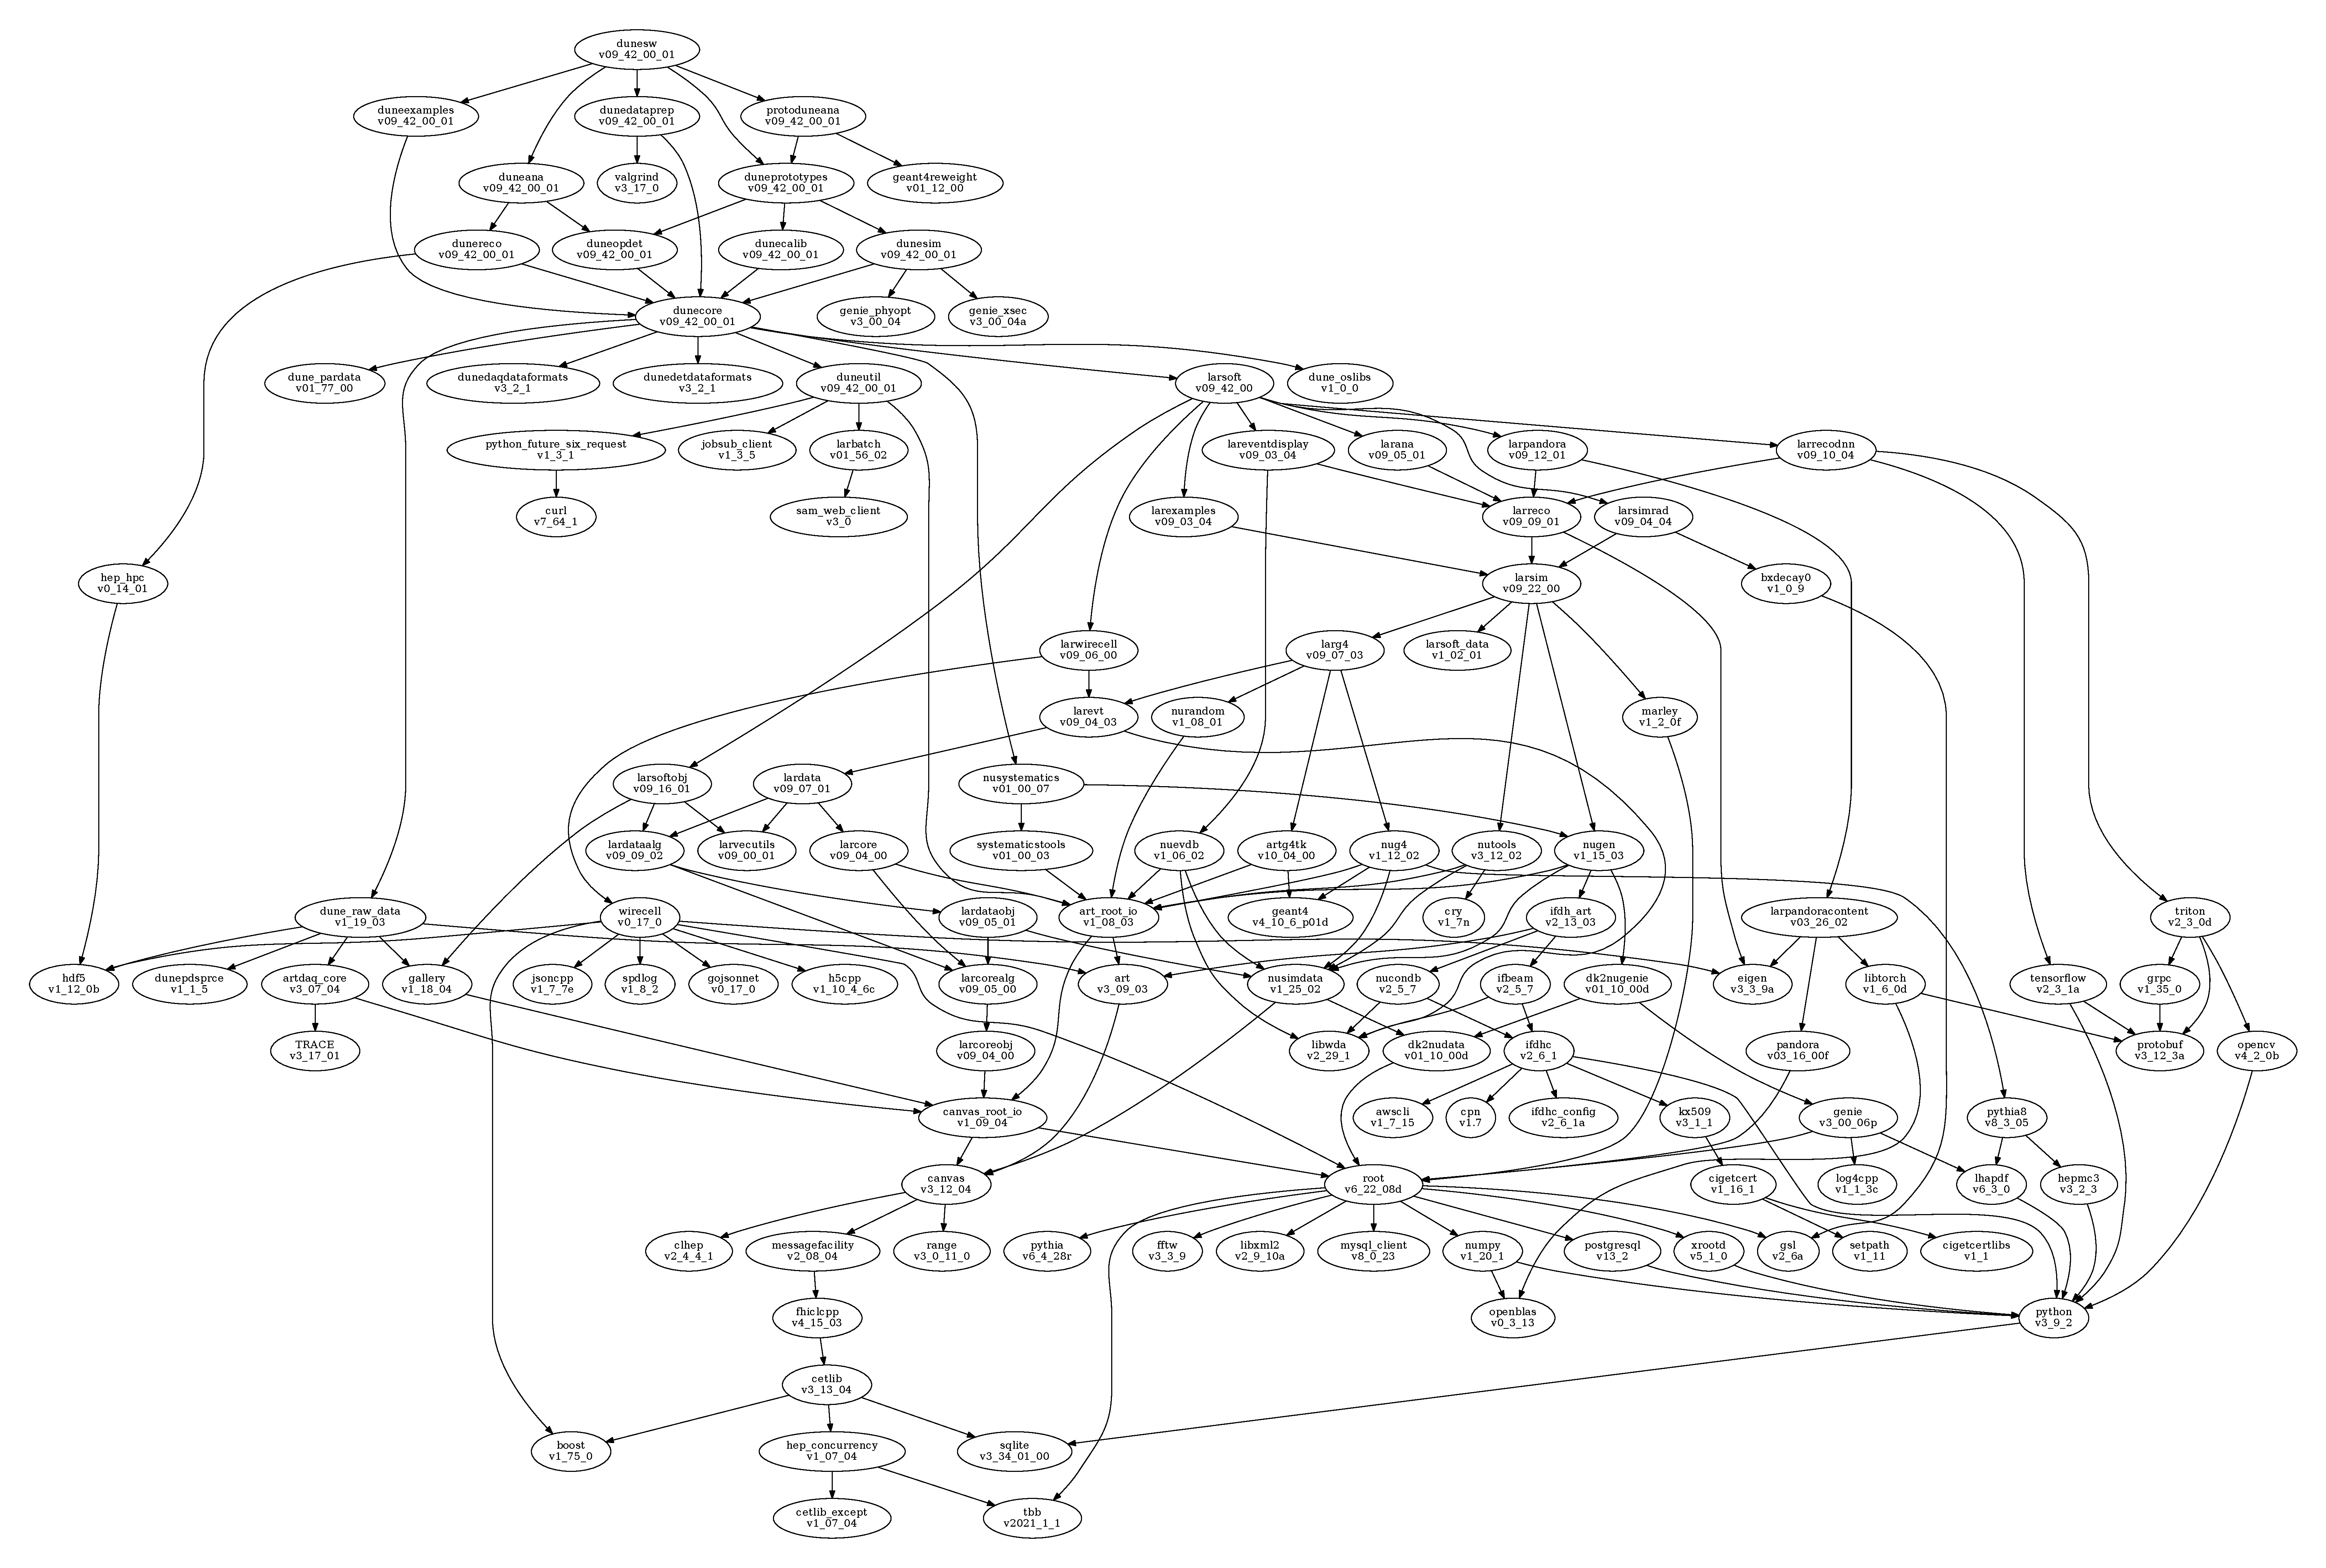
\includegraphics[width=\textwidth]{graphics/CodeManagementFigures/dunesw_v09_42_00_01_graph.pdf}
\end{dunefigure}

Since the dunesw stack depends on LArSoft and sets it up via UPS, dunesw also has a weekly release schedule, and releases are tied to LArSoft's releases and use the same version tag names.  LArSoft's repositories had been hosted in Fermilab's Redmine instance until 2018, at which point they were migrated to GitHub.  At the same time, a pull-request model was instituted.  LArSoft's pull-request system, based on the one used by CMS, performs automated checks that the proposed new code compiles and tests properly.  Once the tests are successful, a review of the proposed new code is required before it can be merged into the repository.  As of this writing, DUNE is considering moving to a pull-request model similar to that of LArSoft.

The build system used is {\tt mrb}, which is provided by and supported by Fermilab's SCD.  Software is built in UPS products which are distributed to the collaboration in two ways.  The primary distribution mechanism is via a set of installed products in CVMFS which can be directly set up by end users without the need to install anything locally.  CVMFS maintains a cache on the user's computer to store copies of the released software files for repeated local access.  CVMFS is also used to distribute released software to batch worker nodes.  The second software distribution mechanism is via the scisoft.fnal.gov web server.  When a release is made, the repositories are tagged and the release manager triggers Fermilab's Jenkins build servers to compile the software and install auxiliary files in UPS products.  The UPS products are then tarred up and the tarballs are uploaded to the scisoft web server, along with a manifest file which describes which tarballs need to be downloaded and installed to get a full, runnable dunesw software stack.

In addition to code, some data files also are distributed via CVMFS.  For example, photon lookup libraries are stored in several-hundred-megabyte rootfiles which are inconvenient to store in a git repository.  They are loaded into a special repository in CVMFS and scisoft called dune\_pardata.  Even larger files are stored in StashCache which has a CVMFS interface for the user, but which retrieves files out of a dedicated area in dCache.

We are evaluating Spack as a replacement for {\tt mrb} and UPS.  Spack is a build system that also allows users to select from a list of installed versions, like UPS.  As operating systems become more secure, some of the ways of distributing, setting up, and running HEP software have conflicted with security features of the operating systems.  One of these is the use of the symbol {\tt LD\_LIBRARY\_PATH}.  UPS uses {\tt LD\_LIBRARY\_PATH} to point a user's environment at directories that contain the versions of released products that can be loaded and run.  Changing the contents of the {\tt LD\_LIBRARY\_PATH} variable causes the same program to load different versions of libraries.  Proper use of UPS maintains compatibility.  However, with newer operating systems, the shared libraries that are linked with programs and other shared libraries must be in the same locations as they where when linked, and not relocated.  The library that links to another keeps track of the installed locations of the libraries it links with.  Alternatively, the paths in which the dependent libraries are found can be edited after installation, in effect re-performing a stage of the linking step.  Spack is aware of this and inserts the proper {\tt rpath} values into linked libraries.

The use of Spack is under evaluation.  UPS is now approximately 25 years old and it is not an industry standard, and it is somewhat linked to Fermilab.  Spack has a significant community using it outside of HEP, and thus there is a large volume of documentation available for it on the web.

%%%%%%%%%%%%%%%%%%%%%%%%%%%%%%%%
\section{Near Detector Code Management \hideme{Muether/Cremonisi/Junk needs update}}
\label{sec:codemgmt:neardet}  %% fix label according to section

The near detector consists of three components.  When DUNE starts running with beam, the expected near detector configuration will be a liquid argon TPC with pixel readout (ND-LAr), a magnetized steel muon spectrometer (TMS), and an on-axis beam monitor, SAND.  A future upgrade is proposed to replace TMS with a gaseous argon TPC with pixel readout, an ECAL and a muon system (ND-GAr). The software structure reflects the detector configuration.  The software effort for each detector has contributions from the groups that are designing and proposing to construct the detectors.  Below is a summary of the code management strategies used for each subsystem, and also for the shared tools.

\subsection{ND-LAr Code Management}
\label{sec:codemgmt:ndlar}

\subsection{TMS Code Management}
\label{sec:codemgmt:tms}

\subsection{ND-GAr Code Management}
\label{sec:codemgmt:ndgar}

The software for simulating and reconstructing events in ND-GAr is, at the time of writing, contained in two repositories:  {\tt garsoft} and {\tt garana}.  GArSoft builds on the functionality of {\it art} and NuTools, and it is maintained when the {\tt art} API changes and when the build system is upgraded.  Following LArSoft's pattern, it is built with {\tt mrb} and set up with {\tt UPS}.   A description of the functionality of GArSoft is in Secs.~\ref{sec:usecases_ndgardetsim} and~\ref{sec:algo:reco:gartpc:pixels}.  GArAna provides a facility for making an analysis ntuple from information stored in GArSoft data products.  Both repositories are hosted at GitHub.  Continuous integration has not yet been set up for GArSoft and GArAna.  Executable binaries and the associated libraries are built using Fermilab's Jenkins build servers, and the build artifacts are installed in CVMFS so that the software can easily be run on the grid.

\begin{dunefigure}
[Dependency graph for the GArSoft software stack. March 2022]
{fig:garsoftdeptree}
{Dependency graph for the GArSoft software stack, for version v02\_16\_00, current as of March 2022.}
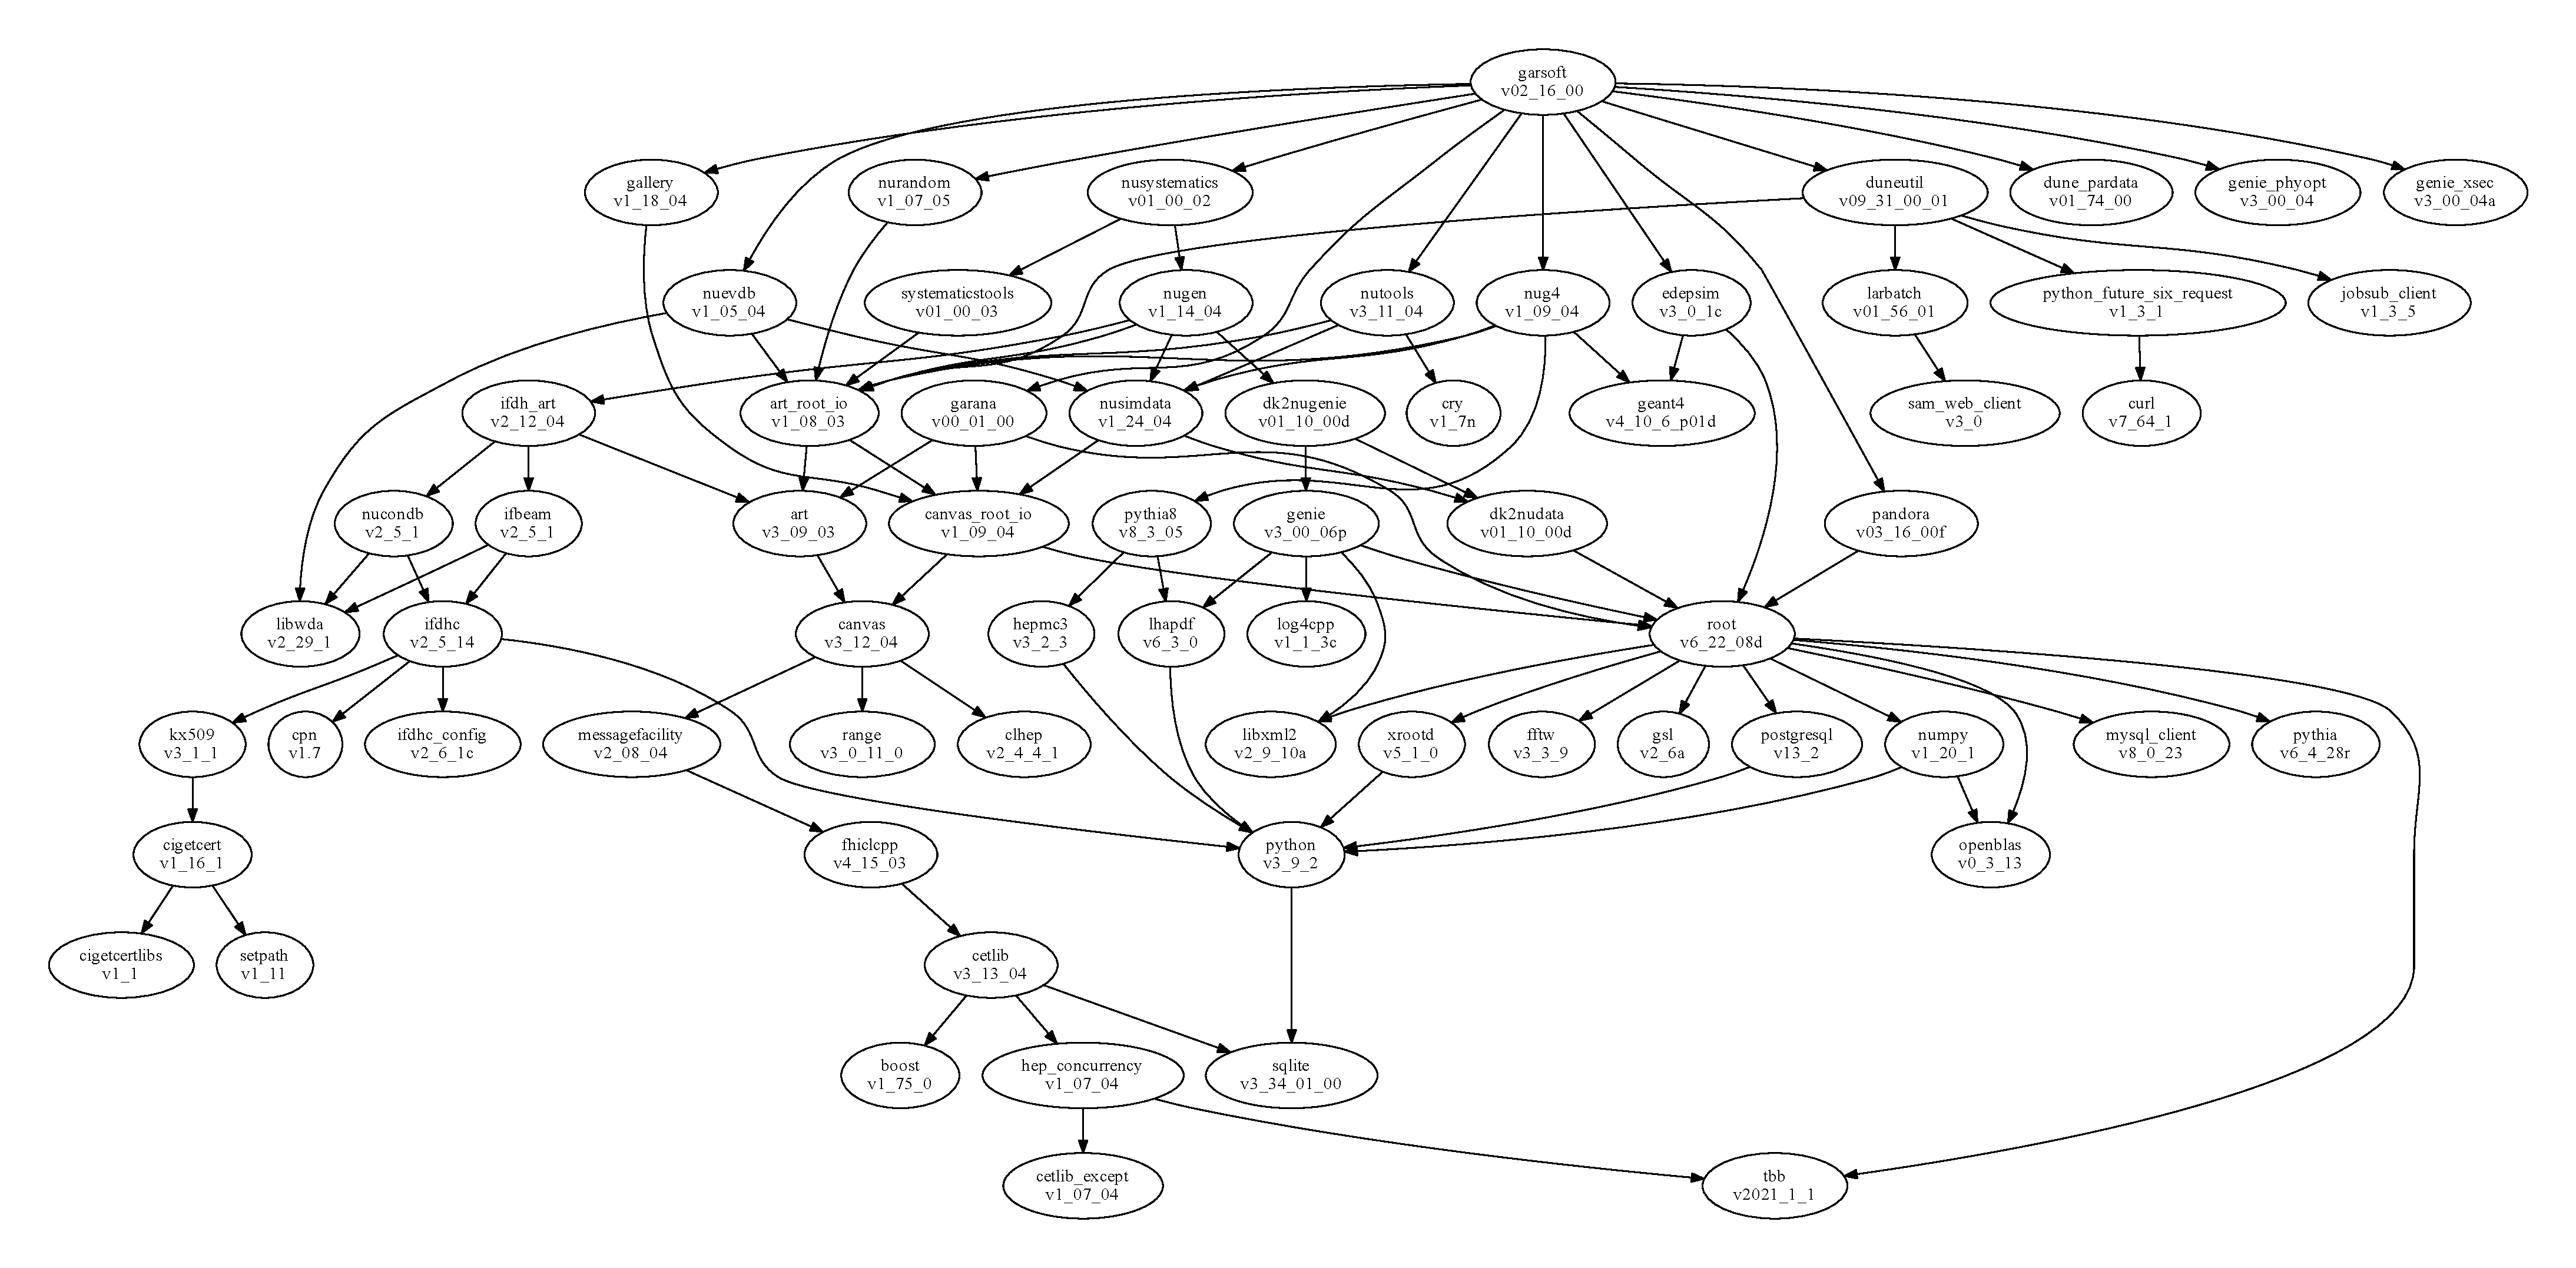
\includegraphics[width=\textwidth]{graphics/CodeManagementFigures/garsoft_v02_16_00_graph.pdf}
\end{dunefigure}

\subsection{SAND Code Management}
\label{sec:codemgmt:sand}

\subsection{Near Detector Production Tools}
\label{sec:codemgmt:ndproduction}

A repository has been set up in GitHub to manage files that are needed for near detector production.  These include production scripts, detector geometry descriptions and flux specifications.  It is versioned and installed in CVMFS like other DUNE repositories, so that production workflows can be reproduced at later dates.

\section{Continuous Integration \hideme{Junk - draft}}
\label{sec:codemgmt:ci}

The stability of the performance of a large base of shared software requires attention to each change that is committed.  Software releases require validation and approval before being used in analyses intended for publication.  The rapid pace of software development early in the life cycle of the experiment, as well as increased activity as data are first collected and conferences come up, requires constant vigilance to ensure that bugs are not introduced and that software remains backwards compatible.

To meet this requirement, an automated continuous integration (CI) system is currently in operation for the LArSoft-based code base.  Similar systems, even using the same infrastructure, will be deployed for the near detector and beam simulations system.  The CI system consists of a set of servers that monitor commits pushed to the central code repositories.  On each commit, with a suitable delay of approximately 15 minutes in order to aggregate commits.  The CI system can also be triggered by user interaction, via an authenticated request.

Once triggered, the CI system will compile the changed code as well as any dependencies that are required.  Currently, the CI system builds LArSoft and all experiment code from the head of the develop branch in the repositories.  This is done because new commits to one repository, be it experiment-specific code or shared LArSoft code, may depend on the latest version of software in other repositories.  If shared software is the subject of the commit, then software that depends on it, such as all the experiment software stacks, are rebuilt, as a change to a header file in a shared repository can cause any source file that includes it, even indirectly, to fail to build.

The status of the build is stored in a logfile and summarized on a web page.  If a commit causes the build to fail, software managers and the person who committed and/or pushed the commit are notified and the commit is blocked from being merged into the head of develop.  LArSoft currently implements a pull-request model, in which experiment-appointed Level-2 managers comment on and sign off on changes to the central code, and Level-1 managers perform the actual merging.  A proposed change will not even be sent out for approval unless the CI system can build it and validation tests are run to compare output that ought not to have been changed by the new code.

This second step, physics performance validation, requires a more lengthy run through both unit tests and integration tests that run simulation and reconstruction workflows.  These tests run on standard input files and have their random number seeds fixed to constants.  The outputs are compared with reference histograms and a web page summarizes the comparison of the output logfiles, histograms, as well as run times and memory consumption, all of which are available on a web site that monitors these tests.  History plots of variables such as run time and memory consumption are made available on the monitoring web site so that investigations of when the memory usage of a job jumped up can be done without laborously checking out, building, and running the software in the suspected timeframe looking for a particular change.
\end{document}
 % Junk and Adams
\cleardoublepage

\part{Resources Summary} %Kirby

%\input{chapters/ro-resource-needs}

%\input{chapters/ro-personnel-needs}

%\input{chapters/ro-work-packages}

\part{Collaboration} 

\documentclass[../main-v1.tex]{subfiles}
\begin{document}
\chapter{Resource Needs Summary}
\label{ch:resource}

\section{Hardware resources}
Chapter \ref{ch:est} described the projected compute and storage needs through 2040, many of which are being met through collaboration contributions. Chapter \ref{ch:netw} describes networking. 



\section{Personnel needs}
Building and managing a project of this complexity also requires a large number of personnel.  Figure \ref{fig:resources} shows a timeline for estimated resource needs.   Efforts are currently spread across a large number of highly expert people working part time on DUNE computing, aside from the five dedicated DOE funded postdocs.  We anticipate that these young people will move into leadership roles in computing in the future.  Although the  FTE are close to the number needed, there is some mis-match in skill-sets. In particular, we anticipate needing several person-years of effort on framework development which is not available with the current mix of personnel.

These roles do not include the large number of people at multiple sites who support generic activites such as storage and grid activities.  The roles listed are people working on \dword{dune} specific projects. 

\subsection{Technical roles}

These roles require substantial computing expertise.  They appear as the darker areas in Figure \ref{fig:resources} adding up to approximately 

\begin{description}


% FTE	2022
% Database administration	0.5
% Database devel. and ops	4
% Data management devel. 	3
% Workload devel. 	1
% Monitoring devel. 	1
% Code management devel. 	1
% Framework devel. 	1
% Analysis devel. 	1
% Data management ops 	2
% Workload ops	2
% Monitoring ops	0.5
% Code management ops	1
% User Support and Documentation	2

\item {Distributed Data Management Development - 2.0 FTE}

This role includes oversight of all software engineering and development activities for packages needed to operate distributed storage resources. The role requires a good understanding of the distributed computing infrastructure used by \dword{dune} as well as the \dword{dune} computing model.

\item {Distributed Computing Development -  2.0 FTE}

This role includes all software engineering and development activities for packages needed to operate  distributed compute resources. The role requires a good understanding of the distributed computing infrastructure used by \dword{dune} as well as the \dword{dune} computing model.

\item {Monitoring Development -  1.0 FTE}

This role includes oversight of all software engineering and development activities for packages needed monitor distributed disk and compute resources. The role requires a good understanding of the distributed computing infrastructure used by \dword{dune} as well as the \dword{dune} computing model.

\item {Database Design and Management - 4.5 FTE}

This role includes designing, maintaining, and scaling databases for  
tasks within \dword{dune}. Considerable effort is needed to interface with the large number of physics, calibration, data acquisition and hardware tasks. People are needed with expertise in databases, data acquisition and project management.  Database operations are included here as they require specialized skills. 

\item {Code Management Development - 1.0 FTE}

The code managers provide infrastructure to support applications for  data processing, simulation, and analysis, and also coordinate activities in the areas of development, release preparation, and %properly
deployment of software package releases needed by \dword{dune}. They organize the overall setup of software packages needed for releases.

The application managers need to keep up with evolution in operating systems, build systems and compilers so this role has a significant development component.

\item{Simulation, reconstruction and analysis frameworks - 3 FTE}
This role requires substantial expertise in the design and deployment of sophisticated frameworks for HEP algorithmic workflows. 


\subsection{Operational  roles}

In addition to the development activities listed above, there are management and operations activities that require management and supervision of collaborators in operations tasks.   These roles are more fluid, based on the status of the experiment and do not always need trained computing personnel but can be filled by collaborators after some training. 
% \item {Central Services Manager and Operators - 1.5 FTE}

% The site manager and operators are responsible for the central infrastructure and services of the \dword{dune} distributed computing infrastructure. This includes coordination with the host laboratory for services provided to \dword{dune}. 

\item {Distributed Production Management - 0.5 FTE}

Distributed production managers are responsible for the setup, launch, monitoring, and %finishing 
completion of processing campaigns executed on distributed computing resources for the experiment. %Production management is necessary for 
These include data processing, \dword{mc} simulation, and working group productions. 


\item {Distributed Data Manager - 0.5 FTE}

The distributed data manager is responsible for operational interactions with distributed computing disk and tape resources. The role includes but is not limited to helping to establish new storage areas and data replication, deletion, and movement. 

\item {Distributed Workload Manager - 0.5 FTE}

The distributed workload manager is responsible for operational interactions with distributed computing resources. The role includes activities such as helping to establish grid and cloud sites. 


\item {Computing Shift Leaders - 1. FTE}

The shift leader is %mainly 
responsible for the experiment's distributed computing operations for a week-long period  %one person covers shifts 
starting on a Monday to the following Sunday.  Shift leaders chair regular operations meetings during their week and attend general \dword{dune} operations meetings as appropriate. %1.4 FTE as it also includes week-ends.

\item {Distributed Computing Resource Contacts - 0.5 FTE}

Distributed computing resource contacts are the primary contacts for the \dword{dune} distributed computing operations team and for the operators of large (Tier-1) sites and regional federations. They interact directly with the computing shift leaders at operations meetings. 

\item {Code Management Operations - 1.0 FTE}

In addition to development associated with changes in systems, code librarians and application managers must continually prepare releases and %properly
deploy  software packages needed by \dword{dune}.  

\item {User Support - 2.0 FTE}

User support (software infrastructure, applications, and distributed computing) underpins all user activities of the \dword{dune} computing project. 
User support %also includes 
personnel %who 
respond to questions from users on mailing lists, Slack-style chat systems, and/or ticketing systems, %as well as documented 
and are responsible for documenting solutions in knowledge bases and wikis.

\item {Resource Board Chair - 0.1 FTE}

This role is responsible for chairing quarterly meetings of the Computing Resource Board, which includes representatives from the %national \dword{dune} collaborations, 
various national funding agencies that support \dword{dune}, to discuss %the level of 
funding for and delivery of the computing resources required for successful processing and exploitation of \dword{dune} data. %0.1 FTE

\item {Computing Coordination - 2.0 FTE}

Coordinators oversee management of the computing project. 
\end{description}



\begin{dunefigure}
[Development Personnel needs]
{fig:resources}
{Estimated computing infrastructure personnel needs through 2030.  The dark colors show development areas where experts are needed while the lighter colors show operations tasks where non-experts can contribute. The dashed line shows the estimated effort allocated to the project.  The bump from 2022-2024 is from a 3-year DOE grant.}
{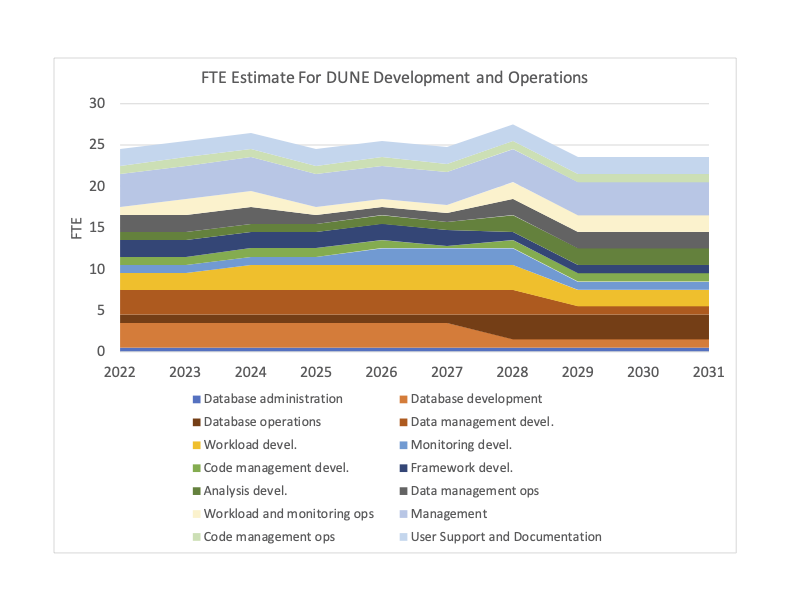
\includegraphics[width=0.9 \textwidth]{graphics/Resources/FTENeeds-2022-02-redo.png}}
\end{dunefigure}
\fixme{HMS - Need to restore the dashed line}
\section{Summary}

This document has described most aspects of \dword{dune} offline computing. Our computing model relies on significant contributions across the collaboration.  

%\hideme{Remove this chapter}
%%%%%%%%%%%%%%%%%%%%%%%%%%%%%%%
%\section{xyz}
%\label{sec:org:xyz}  %% fix label according to section
\end{document}
 %Schellman
\cleardoublepage

\documentclass[../main-v1.tex]{subfiles}
\begin{document}
\chapter{Computing Contributions Board (CCB) \hideme{ Peter Clarke - draft}}
\label{ch:ccb}

%%%%%%%%%%%%%%%%%%%%%%%%%%%%%%%%
%\section{xyz}
%\label{sec:ccb:xyz}  %% fix label according to section

The CCB has been set up to formalize the contribution of DUNE partners to the computing and storage capacity required for computing production. In order to remain scale-able, the CCB considers a nation as the natural unit of aggregation to request and then seek pledges for resources. The CCB does, however, recognize that whilst within some countries centralized coordination is natural, this is not true for others. Nevertheless, requests will be published at a national granularity, with the assumption that Institutes within each nation can coordinate.

In order to set a fair-share request for computing capacity, the CCB will eventually use a proxy metric for the relative proportion of each nation in DUNE. This is likely to be PhD paper authors once in the exploitation phase. This is, however, not relevant during construction as the current listing of DUNE members in the data base is a very poor proxy for this. Therefore, during construction all nations with more than a minimum number of DUNE participants or providing Tier-1 or large Tier-2 capacity to LHC experiments, are asked to provide a "reasonable" share (see below). We refer to these as compute-active-nations.
This is very flexible and is up to each nation to decide if it wishes to be classified as a compute-active-nation.

At present the CCB is composed of a Chair, one member per compute-active-nation, one member for each of FNAL, CERN and BNL, and the Computing and Software Consortium (CSC) Management ex officio.

The CSC management produces an overall requirements document that should be scrutinized by the FNAL CRSG. The CCB receives this document, and then seek pledges to meet those requirements. As host lab, FNAL plans to provide ~25\% of the capacity, including the primary tape service.
CERN also currently provides a substantive capacity, in particular for proto-DUNE.
The aim is then for the remaining capacity to come from other contributors according to the prevailing computing model. A substantial proportion of capacity is expected from outside of the USA  (~50\%). Contributions of at least 5-20\% are requested depending upon the circumstance and capability of each compute-active-nation.
Pledges of capacity received are recorded in the CRIC information system. In due course this process could be formalized into a (non-binding) MOU.

The CCB may also receive requests and information from the CSC Management in respect of any other non-capacity matter. The CCB may seek to help with such requests where they pertain to national contributions. This may include promotion of requests for software engineering support to be propagated within each nation.

\end{document} %Clarke
\cleardoublepage

%\documentclass[../main-v1.tex]{subfiles}
\begin{document}
\chapter{Code Management \hideme{Tom Junk, Mathew Muether, David Adams - draft}}
\label{ch:codemgmt}

\fixme{Doug: ND-LAr TMS and ND-GAr code management sections need to be written, references for CVMFS and Spack need to be found (anne 3/8: dword for cvmfs, spack footnote in prev chap)}

%%%%%%%%%%%%%%%%%%%%%%%%%%%%%%%%
\section{Liquid Argon TPC Code Management \hideme{Junk/Calcutt - needs update}}
\label{sec:codemgmt:dunetpc}  %% fix label according to section

Software for simulation, data read-in, and reconstruction shares significant commonality across the %anne liquid-argon time projection chamber detectors 
DUNE \dwords{lartpc}. %anne planned to be deployed by DUNE and also  prototypes.  
These comprise the %anne horizontal- and vertical-drift far detector modules, the 35-ton prototype, ProtoDUNE-SP, ProtoDUNE-DP, ProtoDUNE-2, ProtoDUNE-VD, ICEBERG, 
the \dword{sphd} and \dword{spvd} \dwords{detmodule}, the \dword{35t}, \dword{pdsp}, \dword{pddp}, \dword{protodune2},  the pixel \dword{nd} and its prototypes.  The same software stack handles the wire readout, the photon detectors, and the cosmic-ray taggers used in some of the prototypes.  The interfaces to event generators, GEANT4, {\it art} and the data handling systems require effort to build and maintain.  Data products need to be thought out carefully.  To reduce the development burden and expand the pool of expertise, DUNE has chosen to use the LArSoft toolkit, which is built on NuTools and {\it art}.  

LArSoft itself is split up into several repositories, such as larcore, larsim, larevt, lardata, and variations that have been split from them over time, such as lardataobj.  LArSoft is supported by Fermilab's Scientific Computing Division and is shared among several other experiments, such as ArgoNeuT, MicroBooNE, ICARUS and SBND.  The pool of developers is quite large, and the rate at which new code is added is quite significant.  New releases of LArSoft are made weekly.  

DUNE's LArSoft-based software historically had been collected in a single git repository called dunetpc, starting in the early days of the collaboration.  This repository was hosted using Fermilab's Redmine service.  Compiling all of the code in this single repository became slower as more source files were added.  In January 2022, a split of the dunetpc repository into ten smaller repositories was deployed on GitHub, taking advantage of GitHub's superior performance, feature set, and openness compared with Redmine.  The old dunetpc repository is kept in a read-only state in Redmine for inspection purposes.  The new top-level product is called dunesw.  A UPS dependency graph made in January 2022 is shown in Figure~\ref{fig:dunetpcdeptree}, showing the dunesw stack, the LArSoft UPS products, and their dependencies.

\begin{dunefigure}
[Dependency graph for the dunesw software stack, Jan 2022]
{fig:dunetpcdeptree}
{UPS dependency graph for the dunesw software stack, for version v09\_42\_00\_01, January 2022.}
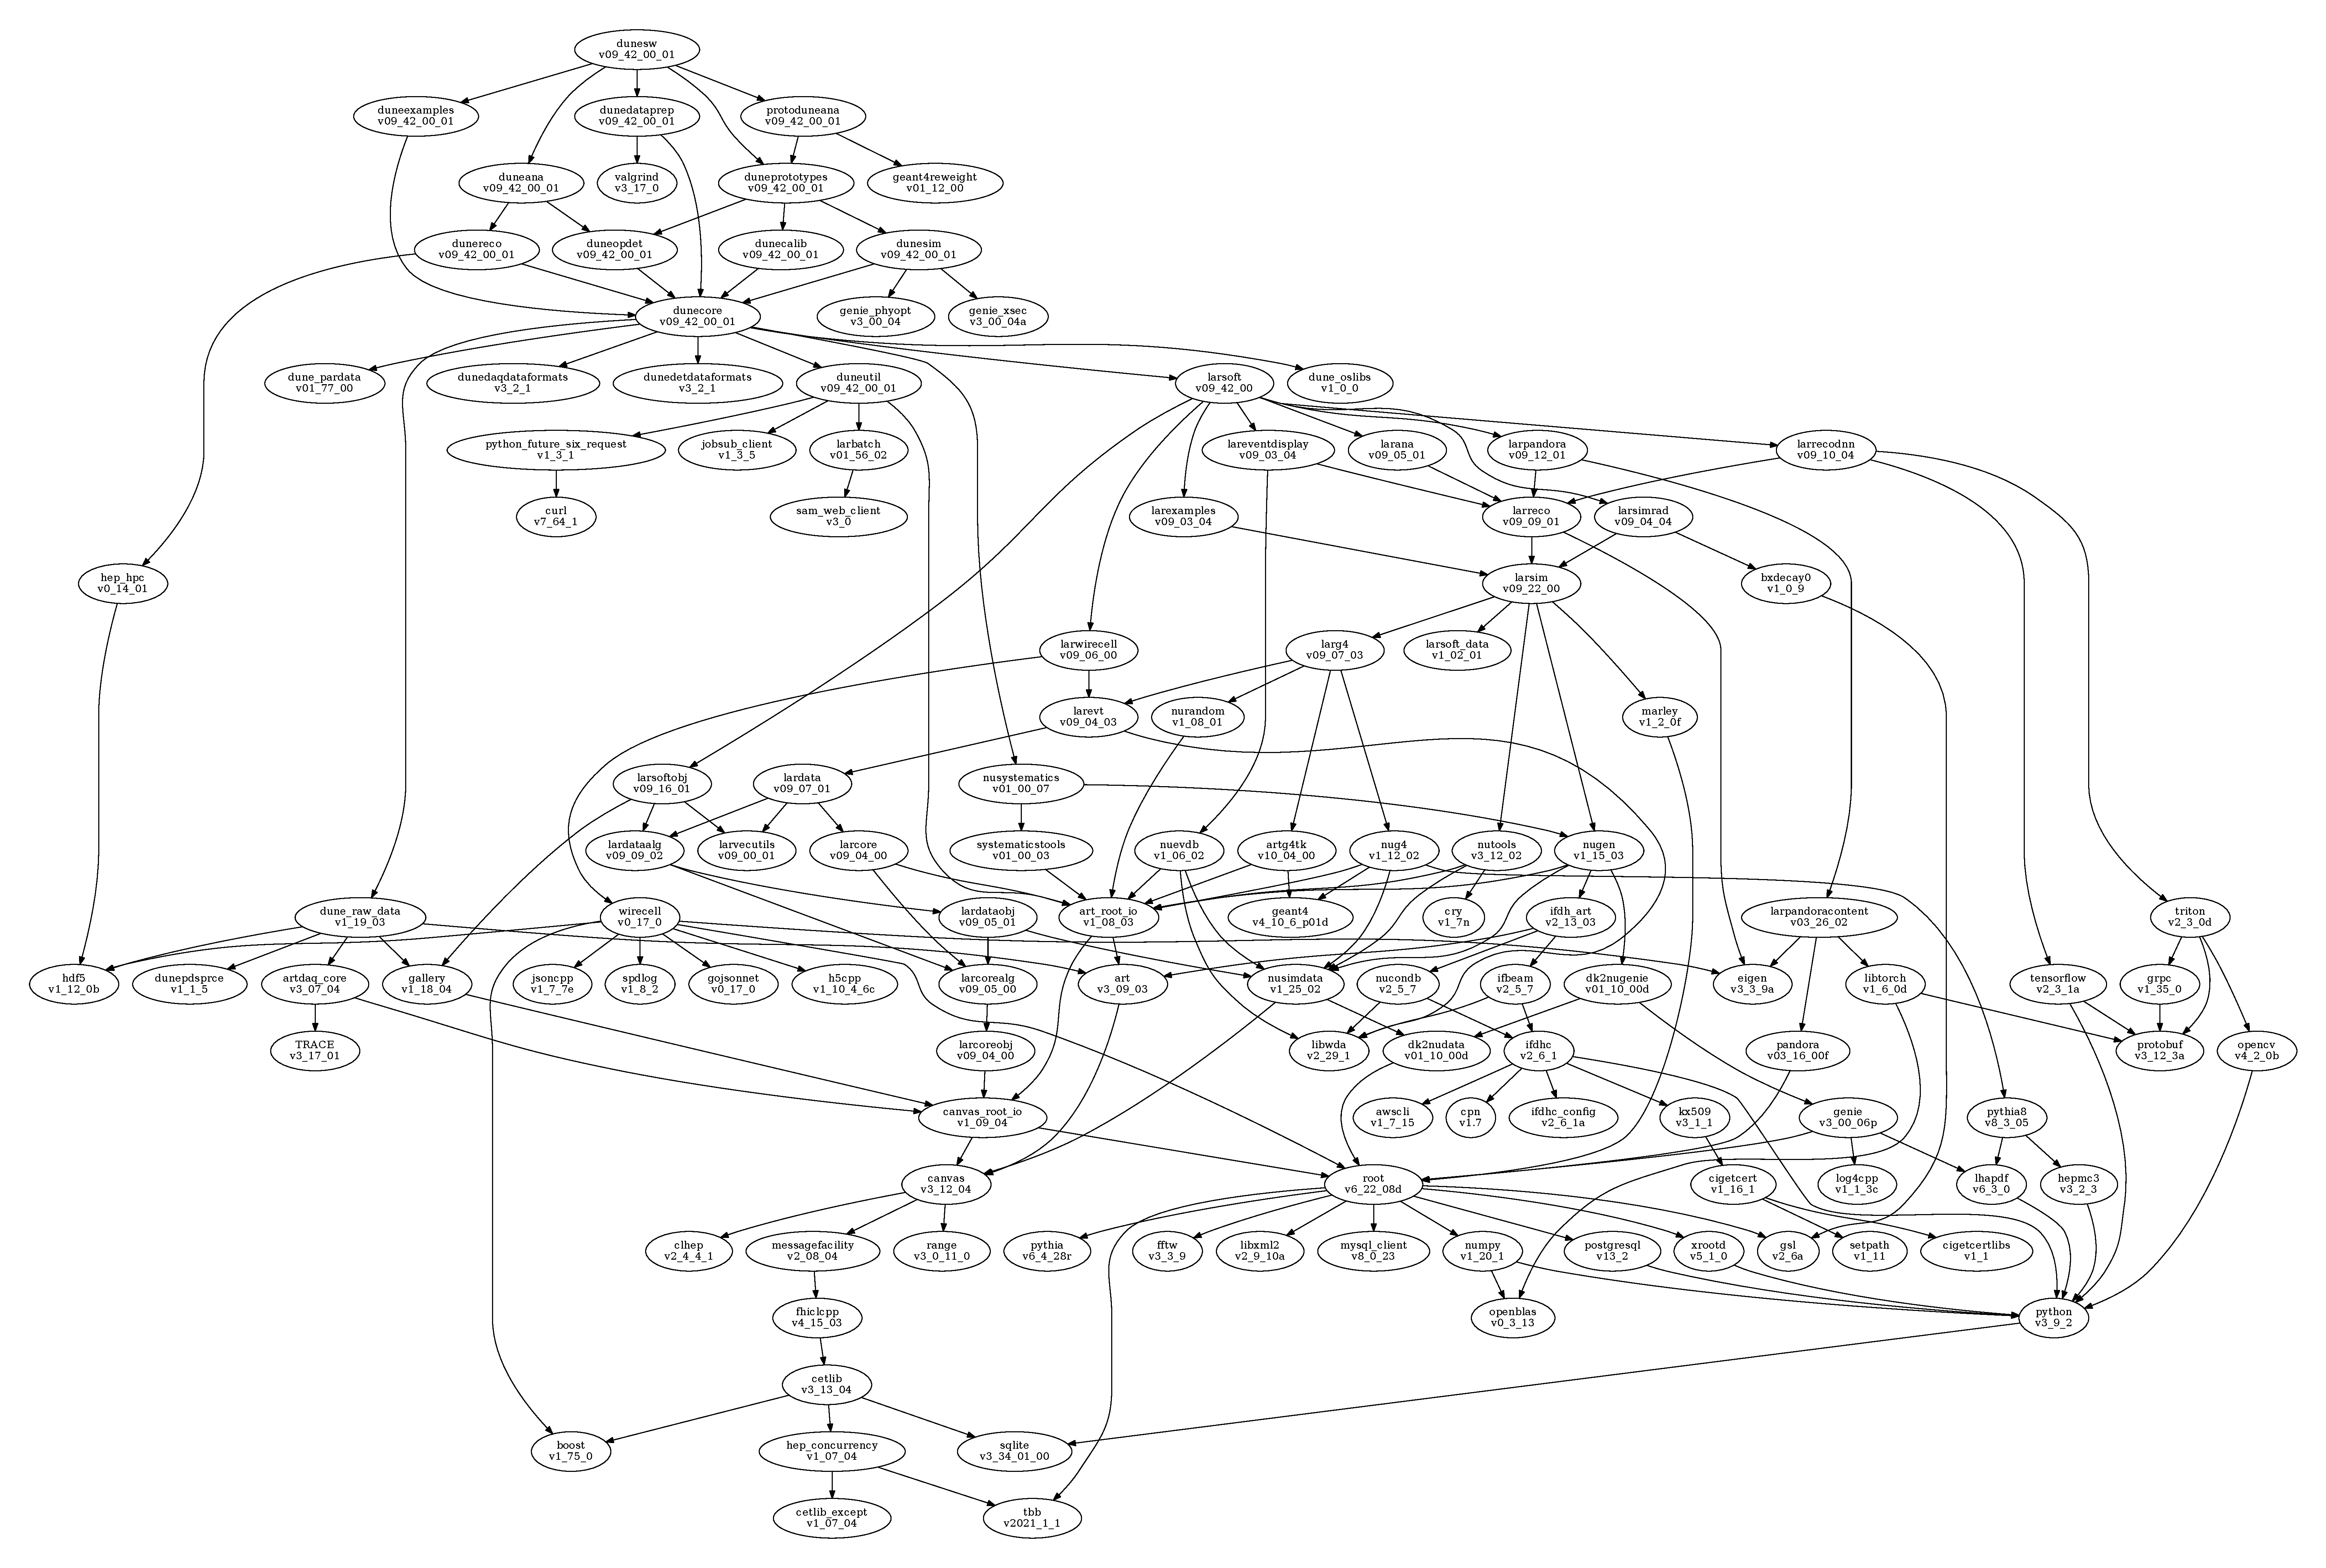
\includegraphics[width=\textwidth]{graphics/CodeManagementFigures/dunesw_v09_42_00_01_graph.pdf}
\end{dunefigure}

Since the dunesw stack depends on LArSoft and sets it up via UPS, dunesw also has a weekly release schedule, and releases are tied to LArSoft's releases and use the same version tag names.  LArSoft's repositories had been hosted in Fermilab's Redmine instance until 2018, at which point they were migrated to GitHub.  At the same time, a pull-request model was instituted.  LArSoft's pull-request system, based on the one used by CMS, performs automated checks that the proposed new code compiles and tests properly.  Once the tests are successful, a review of the proposed new code is required before it can be merged into the repository.  As of this writing, DUNE is considering moving to a pull-request model similar to that of LArSoft.

The build system used is {\tt mrb}, which is provided by and supported by Fermilab's SCD.  Software is built in UPS products which are distributed to the collaboration in two ways.  The primary distribution mechanism is via a set of installed products in CVMFS which can be directly set up by end users without the need to install anything locally.  CVMFS maintains a cache on the user's computer to store copies of the released software files for repeated local access.  CVMFS is also used to distribute released software to batch worker nodes.  The second software distribution mechanism is via the scisoft.fnal.gov web server.  When a release is made, the repositories are tagged and the release manager triggers Fermilab's Jenkins build servers to compile the software and install auxiliary files in UPS products.  The UPS products are then tarred up and the tarballs are uploaded to the scisoft web server, along with a manifest file which describes which tarballs need to be downloaded and installed to get a full, runnable dunesw software stack.

In addition to code, some data files also are distributed via CVMFS.  For example, photon lookup libraries are stored in several-hundred-megabyte rootfiles which are inconvenient to store in a git repository.  They are loaded into a special repository in CVMFS and scisoft called dune\_pardata.  Even larger files are stored in StashCache which has a CVMFS interface for the user, but which retrieves files out of a dedicated area in dCache.

We are evaluating Spack as a replacement for {\tt mrb} and UPS.  Spack is a build system that also allows users to select from a list of installed versions, like UPS.  As operating systems become more secure, some of the ways of distributing, setting up, and running HEP software have conflicted with security features of the operating systems.  One of these is the use of the symbol {\tt LD\_LIBRARY\_PATH}.  UPS uses {\tt LD\_LIBRARY\_PATH} to point a user's environment at directories that contain the versions of released products that can be loaded and run.  Changing the contents of the {\tt LD\_LIBRARY\_PATH} variable causes the same program to load different versions of libraries.  Proper use of UPS maintains compatibility.  However, with newer operating systems, the shared libraries that are linked with programs and other shared libraries must be in the same locations as they where when linked, and not relocated.  The library that links to another keeps track of the installed locations of the libraries it links with.  Alternatively, the paths in which the dependent libraries are found can be edited after installation, in effect re-performing a stage of the linking step.  Spack is aware of this and inserts the proper {\tt rpath} values into linked libraries.

The use of Spack is under evaluation.  UPS is now approximately 25 years old and it is not an industry standard, and it is somewhat linked to Fermilab.  Spack has a significant community using it outside of HEP, and thus there is a large volume of documentation available for it on the web.

%%%%%%%%%%%%%%%%%%%%%%%%%%%%%%%%
\section{Near Detector Code Management \hideme{Muether/Cremonisi/Junk needs update}}
\label{sec:codemgmt:neardet}  %% fix label according to section

The near detector consists of three components.  When DUNE starts running with beam, the expected near detector configuration will be a liquid argon TPC with pixel readout (ND-LAr), a magnetized steel muon spectrometer (TMS), and an on-axis beam monitor, SAND.  A future upgrade is proposed to replace TMS with a gaseous argon TPC with pixel readout, an ECAL and a muon system (ND-GAr). The software structure reflects the detector configuration.  The software effort for each detector has contributions from the groups that are designing and proposing to construct the detectors.  Below is a summary of the code management strategies used for each subsystem, and also for the shared tools.

\subsection{ND-LAr Code Management}
\label{sec:codemgmt:ndlar}

\subsection{TMS Code Management}
\label{sec:codemgmt:tms}

\subsection{ND-GAr Code Management}
\label{sec:codemgmt:ndgar}

The software for simulating and reconstructing events in ND-GAr is, at the time of writing, contained in two repositories:  {\tt garsoft} and {\tt garana}.  GArSoft builds on the functionality of {\it art} and NuTools, and it is maintained when the {\tt art} API changes and when the build system is upgraded.  Following LArSoft's pattern, it is built with {\tt mrb} and set up with {\tt UPS}.   A description of the functionality of GArSoft is in Secs.~\ref{sec:usecases_ndgardetsim} and~\ref{sec:algo:reco:gartpc:pixels}.  GArAna provides a facility for making an analysis ntuple from information stored in GArSoft data products.  Both repositories are hosted at GitHub.  Continuous integration has not yet been set up for GArSoft and GArAna.  Executable binaries and the associated libraries are built using Fermilab's Jenkins build servers, and the build artifacts are installed in CVMFS so that the software can easily be run on the grid.

\begin{dunefigure}
[Dependency graph for the GArSoft software stack. March 2022]
{fig:garsoftdeptree}
{Dependency graph for the GArSoft software stack, for version v02\_16\_00, current as of March 2022.}
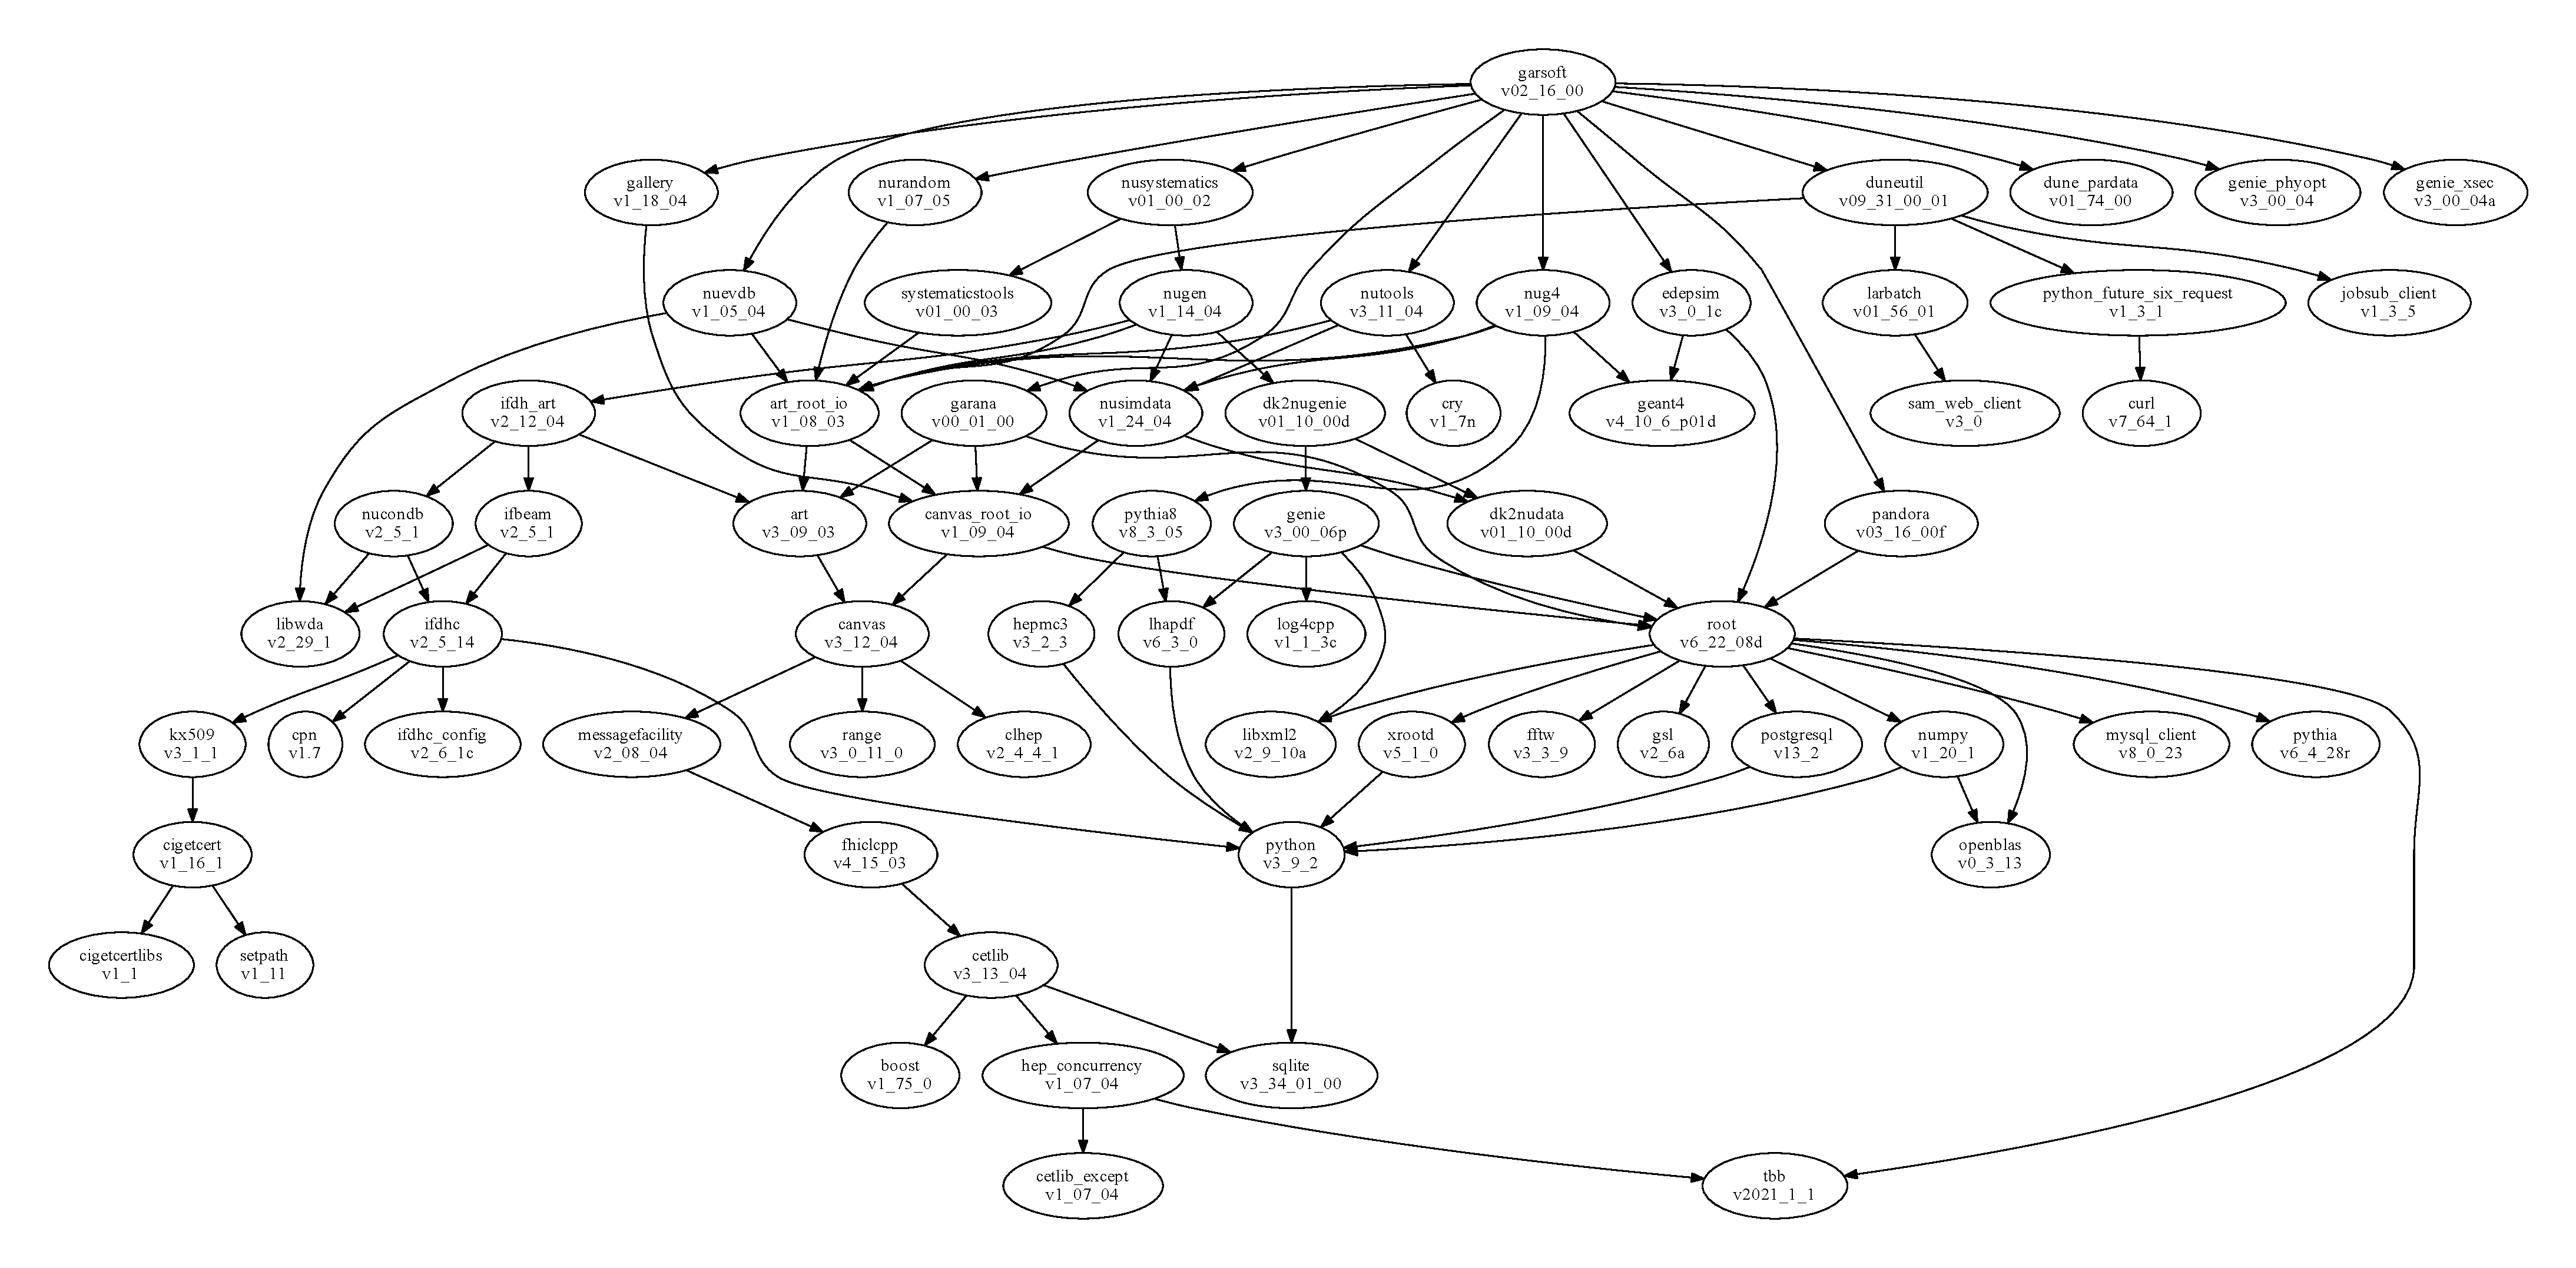
\includegraphics[width=\textwidth]{graphics/CodeManagementFigures/garsoft_v02_16_00_graph.pdf}
\end{dunefigure}

\subsection{SAND Code Management}
\label{sec:codemgmt:sand}

\subsection{Near Detector Production Tools}
\label{sec:codemgmt:ndproduction}

A repository has been set up in GitHub to manage files that are needed for near detector production.  These include production scripts, detector geometry descriptions and flux specifications.  It is versioned and installed in CVMFS like other DUNE repositories, so that production workflows can be reproduced at later dates.

\section{Continuous Integration \hideme{Junk - draft}}
\label{sec:codemgmt:ci}

The stability of the performance of a large base of shared software requires attention to each change that is committed.  Software releases require validation and approval before being used in analyses intended for publication.  The rapid pace of software development early in the life cycle of the experiment, as well as increased activity as data are first collected and conferences come up, requires constant vigilance to ensure that bugs are not introduced and that software remains backwards compatible.

To meet this requirement, an automated continuous integration (CI) system is currently in operation for the LArSoft-based code base.  Similar systems, even using the same infrastructure, will be deployed for the near detector and beam simulations system.  The CI system consists of a set of servers that monitor commits pushed to the central code repositories.  On each commit, with a suitable delay of approximately 15 minutes in order to aggregate commits.  The CI system can also be triggered by user interaction, via an authenticated request.

Once triggered, the CI system will compile the changed code as well as any dependencies that are required.  Currently, the CI system builds LArSoft and all experiment code from the head of the develop branch in the repositories.  This is done because new commits to one repository, be it experiment-specific code or shared LArSoft code, may depend on the latest version of software in other repositories.  If shared software is the subject of the commit, then software that depends on it, such as all the experiment software stacks, are rebuilt, as a change to a header file in a shared repository can cause any source file that includes it, even indirectly, to fail to build.

The status of the build is stored in a logfile and summarized on a web page.  If a commit causes the build to fail, software managers and the person who committed and/or pushed the commit are notified and the commit is blocked from being merged into the head of develop.  LArSoft currently implements a pull-request model, in which experiment-appointed Level-2 managers comment on and sign off on changes to the central code, and Level-1 managers perform the actual merging.  A proposed change will not even be sent out for approval unless the CI system can build it and validation tests are run to compare output that ought not to have been changed by the new code.

This second step, physics performance validation, requires a more lengthy run through both unit tests and integration tests that run simulation and reconstruction workflows.  These tests run on standard input files and have their random number seeds fixed to constants.  The outputs are compared with reference histograms and a web page summarizes the comparison of the output logfiles, histograms, as well as run times and memory consumption, all of which are available on a web site that monitors these tests.  History plots of variables such as run time and memory consumption are made available on the monitoring web site so that investigations of when the memory usage of a job jumped up can be done without laborously checking out, building, and running the software in the suspected timeframe looking for a particular change.
\end{document}
 % Junk and Adams
%\cleardoublepage

\chapter{Training and Documentation \hideme{Claire David, Mike Kirby}}
\label{ch:train}
%%%%%%%%%%%%%%%%%%%%%%%%%%%%%%%%
%\section{xyz}
%\label{sec:train:xyz}  %% fix label according to section
DUNE is a rapidly growing collaboration from almost 200 institutions. The scale of the experiment demands a harmonized documentation effort, coupled with consistent training for both newcomers and existing users. Although treated separately in this section, the tasks of documentation and training are highly correlated. Both are crucial for the long term success of DUNE. 

\section{Documentation}
The documentation related to the DUNE’s computing aspects will be accessible on a variety of platforms, each with specific goals and access policies.

\subsection{Wikis}
The existing DUNE wiki acts as the landing page and starting point for ``DUNE Computing." It acts as a portal gathering information and links about the DUNE Computing consortium groups, its activities and related resources. The template has been revamped in early 2021 with a ‘block’ design for a more visual and compact layout. As with the rest of the DUNE wiki, its access is restricted; users need a FNAL Single Sign-On (SSO) service domain since the wiki contains information about computing access, node names, and other sensitive information.

A separate publicly accessible wiki for DUNE Computing is in preparation. The motivations for a dedicated public page are to make the information available for associated collaborations (e.g. OSG, WLCG, HSF), have a point of contact for newcomers not yet registered, and show the DUNE Computing activities to the outside world in general. This public portal has six main blocks: management, operation, getting started, user area, developer area, documentation. The management block informs about the consortium, the calendar of meetings, and list the associated collaborations. The operation block redirects to monitoring pages essential during data taking and/or production (FIFEmon tools). The block ‘getting started’ will have pointers on the tutorials, training sessions and how-tos. The block 'user area' collects links about analysis tools, framework, and helpdesk. The DUNE Computing working groups are listed on the developer area, and conveners of each working group will maintain their page. Last but not least, the documentation block gathers links about data policies and preservation, information protection, and the documents in progress.

Critical information such as login commands or computer node names will not be visible on the public wiki. Instead, the public wiki will provide links pointing to an access-restricted page on DUNE’s main wiki where details can be safely provided. Only users with approved DUNE credentials will be able to access them. The public wiki will not duplicate the information but rather offer a summary to the outside world, benefiting visitors from founding agencies and future DUNE’s newcomers, not to mention the potential to foster collaborations with scientists from other experiments.

\subsection{Redmine}
The current primary repository for DUNE Far Detector and ProtoDUNE software is the dunetpc repository that is accessed through the FNAL Redmine service. Along with the code repository, there is issue tracking and a wiki embedded within the service. This service will likely be retired within the 2021 calendar year and therefore work is on going to transition away from the Redmine service. The contents of the wiki will be transferred to the access-restricted DUNE wiki discussed previously, while the issue tracking will be transitioned to Github.

\subsection{Code Documentation}
One of the challenges for any large experiment is documentation of the algorithms and software. Following the lead of the Belle2 experiment, DUNE plans to explore the implementation of the Sphynx\footnote{https://www.sphinx-doc.org/en/master/} package for the automatic generation of code documentation. The generation of in-code comments and dedicated text files utilized by Sphynx will be the responsibility of code librarians and contributors of each sub-repository within the dunetpc code stack.

\subsection{GitHub}
DUNE software is migrating to the version-controlled platform GitHub, offering a ticketing system facilitating debugging, revisions and updates from the community of users. The work to make this transition is underway and is following the guidance of the HSF community. Issues of access, privacy, and de-authorization of accounts are currently under investigation and it has not yet been determined what the future policy shall be.

\section{Training}

\subsection{Goals of DUNE Training}
DUNE’s training aims at serving both newcomers and existing users, offering a smooth start for the former and continuous support for the latter. DUNE recognizes that the computing environment and tools utilized within an HEP experiment are unique and require specialized training. The goals are to teach the basics of the environment and software used for analysis, as well as best practices in programming and data management. The training is offered through various formats and platforms, as well as tools and collaborations, all discussed below. 

\subsection{Training sessions}
The primary training for new DUNE members is done twice a year during several- day-long dedicated sessions. These sessions are coordinated with the collaboration week, occurring alternatively before or after. Such timing secures a good attendance for both newcomers and lecturing experts.
The format of the training is an alternation of lectures and  hands-on sessions. Introductory instructions and preliminary homework are sent to participants before the tutorials to ensure the trainees arrive with access to computing resources, one of the primary hurdles to learning about and using new computing environments.

General topics such as DUNE computing basics and grid job submission will be covered each year. However, due to the vast suite of software used by the DUNE collaboration for the various analysis steps and sub-detectors, each event will highlight a particular software package or analysis toolkit. All past tutorials will be thoroughly documented to serve as self-education material, providing an asynchronous training for newcomers having missed a previous session.

\subsection{Training tools}
The past sessions have used the wiki as main support for the training material. The lectures proceed through a dedicated wiki page containing informative sections, sets of commands to run and numerous links pointing to further reading.

The DUNE Computing training group plans to create a dedicated FAQ platform. It would be similar to  Askbot\footnote{https://askbot.org}, an open source software offering user support with a question database whose answers are rated by relevance and popularity (inspired by the source-based websites Reddit and Stackoverflow). This choice is motivated by the positive feedback of the training organized in January 2021. Askbot is no longer available, so for now live documents (hosted on GoogleDoc) were shared to welcome questions from the participants. The anonymity is a key feature. Participants could ask anonymously, a key feature as many young members are usually not daring to ask. Experts then provide written answers. The numerous questions with their answers are later added to the tutorial wiki pages. Following this success, a dedicated FAQ instance would be an efficient, crowd-based, and self-maintained platform to eventually collect the most frequently asked questions, while offering the most relevant answers or solutions.

In the future, DUNE has the goal that training events will utilize Jupyter notebooks, and therefore provide an interactive environment for the trainees to run the examples, do exercises, and tweak portions of code to deepen their understanding of the analysis software. These notebooks will be accessible through a JupyterHub server provided by FNAL and CERN, as well as other hosting institutions equipped with computing resources and analysis facility tools. The notebooks will be archived and referenced on the wiki as self-training modules for newcomers as well as inspiration material for young lecturers.

Lectures will be recorded and the link of the video will be posted on the wiki or a dedicated platform. The training sessions will thus be available asynchronously at any time.

\subsection{Partnering with other collaborations}
The HEP Software Foundation (HSF) has started a continuous effort of harmonizing their tutorials under a common template called “training module.” The HSF aims at creating an introductory curriculum giving HEP newcomers the basic set of software needed while instilling good programming practices right at the start. Several of their modules for beginners are offered by the Software Carpentry Foundation\footnote{https://software-carpentry.org }. The growing list of modules can be found on the HSF website “Towards a HEP Software Training curriculum"~\footnote{https://hepsoftwarefoundation.org/training/curriculum.html}.

The DUNE Computing training group will work in collaboration with the HSF, pointing newcomers to the curriculum as part of the prerequisites before attending an official DUNE training. This will give the HSF an audience to their self-serve training centre, which in return provide valuable feedback and thus the opportunity to improve and fine-tune their HSF tutorials. In the middle term, the neutrino specifics can be introduced for HSF and bring a diversity in their curriculum.

\subsection{From trainee to mentor, user to lecturer}
A key aspect of the success of the HSF workshops resides in its mentoring system. Participants are split in small groups with one mentor to assist the students. The mentors are young researchers and alumni of the previous training session. This facilitates communication as newcomers are less reluctant to ask questions. After a couple of training sessions, the mentors can be trained by experts to become lecturers, acquiring new skills with their favorite software. The DUNE Computing consortium plans to reproduce the HSF mentoring and training scheme with frequent calls for mentors within the collaboration.

\subsection{Future formats}
The DUNE Computing training group is also committed in surveying the needs and various demands for particular aspects and skills the members would like to learn. Recent surveys have shown that LArSoft and Pandora are popular topics, that there is a general interest to know the ‘best practices’ for building analysis code, not to mention learning about machine learning techniques (Keras, Tensorflow, GPU libraries). The breadth of the tutorial wish-list is too large to efficiently cover during one bi-annual DUNE training, but continued input from tutorial attendees allow the planning of future topic specific lectures and tutorials. Moreover, incoming students are each working on a specific aspect of the DUNE project. A project-based approach such as a hackathon would be an ideal format for the training, where students would team up on an aspect directly linked with their analysis. They “go back home” with a program directly needed for their research. The presence of an expert to give them early guidance would be greatly beneficial as it would instill good practices while building the student confidence as a future analyzer. An experimental hackathon training will be organized in 2021 to test this format for the coming years.



%Training Considerations (brainstorming w/ myself to verify Overleaf privs - DeMuth)
%\begin{itemize}
%    \item Introduction to High Performance Computing
%    \item \LaTeX ~documentation, tables, and figures
%    \item GitHub Usage
%    \item DUNE Collaboration DB
%    \item Shifters
%\end{itemize}

 % David
\cleardoublepage

\part{Summary and Plans}

\fixme{Where do personnel needs go?}


% this is added just after end of document

\cleardoublepage
\printglossaries

\cleardoublepage
%begin stuff from init per Thomas 6/2/2106
% end stuff from init
\cleardoublepage
\renewcommand{\bibname}{References}
\bibliographystyle{utphys} 
% To understand the style chosen, see:
% https://arxiv.org/hypertex/bibstyles/ (very bottom -- additions) and
% https://www.sharelatex.com/learn/Bibtex_bibliography_styles
% July 2017, AH and BV (and AM)
\bibliography{common/tdr-citedb}

\end{document}
